% Options for packages loaded elsewhere
\PassOptionsToPackage{unicode}{hyperref}
\PassOptionsToPackage{hyphens}{url}
\PassOptionsToPackage{dvipsnames,svgnames,x11names}{xcolor}
%
\documentclass[
  letterpaper,
  DIV=11,
  numbers=noendperiod]{scrartcl}

\usepackage{amsmath,amssymb}
\usepackage{setspace}
\usepackage{iftex}
\ifPDFTeX
  \usepackage[T1]{fontenc}
  \usepackage[utf8]{inputenc}
  \usepackage{textcomp} % provide euro and other symbols
\else % if luatex or xetex
  \usepackage{unicode-math}
  \defaultfontfeatures{Scale=MatchLowercase}
  \defaultfontfeatures[\rmfamily]{Ligatures=TeX,Scale=1}
\fi
\usepackage{lmodern}
\ifPDFTeX\else  
    % xetex/luatex font selection
\fi
% Use upquote if available, for straight quotes in verbatim environments
\IfFileExists{upquote.sty}{\usepackage{upquote}}{}
\IfFileExists{microtype.sty}{% use microtype if available
  \usepackage[]{microtype}
  \UseMicrotypeSet[protrusion]{basicmath} % disable protrusion for tt fonts
}{}
\usepackage{xcolor}
\setlength{\emergencystretch}{3em} % prevent overfull lines
\setcounter{secnumdepth}{5}
% Make \paragraph and \subparagraph free-standing
\ifx\paragraph\undefined\else
  \let\oldparagraph\paragraph
  \renewcommand{\paragraph}[1]{\oldparagraph{#1}\mbox{}}
\fi
\ifx\subparagraph\undefined\else
  \let\oldsubparagraph\subparagraph
  \renewcommand{\subparagraph}[1]{\oldsubparagraph{#1}\mbox{}}
\fi


\providecommand{\tightlist}{%
  \setlength{\itemsep}{0pt}\setlength{\parskip}{0pt}}\usepackage{longtable,booktabs,array}
\usepackage{calc} % for calculating minipage widths
% Correct order of tables after \paragraph or \subparagraph
\usepackage{etoolbox}
\makeatletter
\patchcmd\longtable{\par}{\if@noskipsec\mbox{}\fi\par}{}{}
\makeatother
% Allow footnotes in longtable head/foot
\IfFileExists{footnotehyper.sty}{\usepackage{footnotehyper}}{\usepackage{footnote}}
\makesavenoteenv{longtable}
\usepackage{graphicx}
\makeatletter
\def\maxwidth{\ifdim\Gin@nat@width>\linewidth\linewidth\else\Gin@nat@width\fi}
\def\maxheight{\ifdim\Gin@nat@height>\textheight\textheight\else\Gin@nat@height\fi}
\makeatother
% Scale images if necessary, so that they will not overflow the page
% margins by default, and it is still possible to overwrite the defaults
% using explicit options in \includegraphics[width, height, ...]{}
\setkeys{Gin}{width=\maxwidth,height=\maxheight,keepaspectratio}
% Set default figure placement to htbp
\makeatletter
\def\fps@figure{htbp}
\makeatother

\usepackage{fontspec}
\usepackage{multirow}
\usepackage{multicol}
\usepackage{colortbl}
\usepackage{hhline}
\newlength\Oldarrayrulewidth
\newlength\Oldtabcolsep
\usepackage{longtable}
\usepackage{array}
\usepackage{hyperref}
\usepackage{float}
\usepackage{wrapfig}
% \usepackage{hyperref}
% \hypersetup{
%     colorlinks,
%     linkcolor={blue!100!black},
%     citecolor={blue!100!black},
%     urlcolor={blue!100!black}
% }
% \usepackage{apacite}
% \usepackage[round]{natbib} 
% \usepackage{graphicx}
% \usepackage{float}
% \usepackage{caption}
% \usepackage[toc,page]{appendix}
% \usepackage{booktabs,caption}
% \usepackage[flushleft]{threeparttable}
% \usepackage{tabularx}
\usepackage{sfmath}
\usepackage{fontspec}
\usepackage[utf8]{inputenc}
\usepackage{siunitx}
\usepackage{amsfonts}
\usepackage{amsmath}
% \usepackage{xcolor}
% \usepackage{scrextend}
% \deffootnote[2em]{2em}{1em}{\textsuperscript{\thefootnotemark}\,}
% \newcolumntype{Y}{>{\centering\arraybackslash}X}
% \usepackage[a4paper]{geometry}
% \usepackage{caption}
% \usepackage[bottom,flushmargin,hang,multiple]{footmisc}
% \usepackage{pdflscape}
% \usepackage[paper=portrait,pagesize]{typearea}
% \usepackage{rotating}
% \usepackage{fullpage}
% \usepackage{tabu}
\usepackage{lscape}
\newcommand{\blandscape}{\begin{landscape}}
\newcommand{\elandscape}{\end{landscape}}
\usepackage{rotating}
\newcommand{\bsideways}{\begin{sidewaystable}[htbp]}
\newcommand{\esideways}{\end{sidewaystable}}
\KOMAoption{captions}{tableheading}
\makeatletter
\@ifpackageloaded{caption}{}{\usepackage{caption}}
\AtBeginDocument{%
\ifdefined\contentsname
  \renewcommand*\contentsname{Table of contents}
\else
  \newcommand\contentsname{Table of contents}
\fi
\ifdefined\listfigurename
  \renewcommand*\listfigurename{List of Figures}
\else
  \newcommand\listfigurename{List of Figures}
\fi
\ifdefined\listtablename
  \renewcommand*\listtablename{List of Tables}
\else
  \newcommand\listtablename{List of Tables}
\fi
\ifdefined\figurename
  \renewcommand*\figurename{Figure}
\else
  \newcommand\figurename{Figure}
\fi
\ifdefined\tablename
  \renewcommand*\tablename{Table}
\else
  \newcommand\tablename{Table}
\fi
}
\@ifpackageloaded{float}{}{\usepackage{float}}
\floatstyle{ruled}
\@ifundefined{c@chapter}{\newfloat{codelisting}{h}{lop}}{\newfloat{codelisting}{h}{lop}[chapter]}
\floatname{codelisting}{Listing}
\newcommand*\listoflistings{\listof{codelisting}{List of Listings}}
\makeatother
\makeatletter
\makeatother
\makeatletter
\@ifpackageloaded{caption}{}{\usepackage{caption}}
\@ifpackageloaded{subcaption}{}{\usepackage{subcaption}}
\makeatother
\ifLuaTeX
  \usepackage{selnolig}  % disable illegal ligatures
\fi
\usepackage[round]{natbib}
\bibliographystyle{apalike}
\usepackage{bookmark}

\IfFileExists{xurl.sty}{\usepackage{xurl}}{} % add URL line breaks if available
\urlstyle{same} % disable monospaced font for URLs
\hypersetup{
  colorlinks=true,
  linkcolor={blue!000!black},
  filecolor={Maroon},
  citecolor={blue!000!black},
  urlcolor={blue!000!black},
  pdfcreator={LaTeX via pandoc}}

\author{}
\date{}

\begin{document}

\title{Regulation and bank lending in South Africa: A narrative index approach\thanks{The authors thank the South African Reserve Bank for their financial assistance. This paper is provided as part of the Bank's call for papers on the impact of prudential regulation on financial services. We also thank Sanelisiwe Hlatshwayo for invaluable research assistance.}}

\author {Xolani Sibande\footnote{Economic Research Department, South African Reserve Bank; Email: xolani.sibande@resbank.co.za.} \and
Dumakude Nxumalo\footnote{Department of Economics, University of Pretoria, Pretoria, South Africa; Email: dumakude.nxumalo@up.ac.za} \and
Keaoleboga Mncube\footnote{Department of Economics, University of Pretoria, Pretoria, South Africa; Email: keaolebogamncube@gmail.com} \and
Steve Koch\footnote{Department of Economics, University of Pretoria, Pretoria, South Africa; Email: steve.koch@up.ac.za} \and
Nicola Viegi\footnote{Department of Economics, University of Pretoria, Pretoria, South Africa; Email: viegin@gmail.com}}

\date{\today}
\maketitle

\begin{center}
\textbf{Abstract}
\end{center}

\begin{abstract}
This study estimates and contrasts the impact of potentially contradictory regulation on the bank lending rates and volumes of the South Africa's largest banks. The regulations we consider are macroprudential regulation that seek to achieve stability in the finance sector and finance regulations intended to achieve greater financial inclusion.  We estimate separate panel data regressions for the different types of regulations we consider. Our results suggest that macroprudential policy is working as intended as it is associated with increases in interest rates on unsecured lending rates, decreases in short-term secured and mortgage lending rates. We observe that lending growth rates in unsecured and secured credit increase and decrease in mortage lending. Inclusion focused regulation is associated with increased bank lending rates in unsecured credit and lower mortgage rates. We observe a decrease in the growth of unsecured lending for corporates and an increase in secured lending for corporates. Results suggest inclusion focused regulation is at odds with its objectives and is consistent with the impact of macroprudential policy on bank pricing.
\end{abstract}


\noindent\textbf{Keywords}: Bank lending, narrative methods, finance regulation\\
\textbf{JEL Codes}: G01, G18, G28, G32, G38
\newpage

\setstretch{1.5}
\section{Introduction}\label{introduction}

Macroprudential policies are pursued in order to achieve stability in
the finance sector. These policies could consist of higher bank capital
requirements that ultimately lower lending in order to meet said
requirements. The South African government has also sought to achieve
greater levels of financial inclusion, largely through finance sector
regulatory reforms. One of the primary ways of enhancing inclusion is
through the extension of affordable credit to those who may have poor
access or may have been excluded in the ordinary course. The existence
of these two types of policies potentially suggest that their
application may be at odds. Our paper therefore first analyses whether
the realised impacts of regulatory developments related to
macroprudential policy and financial inclusion meet their intended
goals. Secondly, we consider whether the two regulatory approaches are
potentially contradictory.

We achieve this through a panel data approach to estimate the impact of
the different regulatory developments on bank rates and three month
changes in bank lending volumes. To measure regulatory developments, we
develop narrative indices that comprehensively measure all developments
relevant to our study. This approach is consistent with various studies
that consider the effect of macroprudential reforms on the stock of
lending. However, this paper extends this type of analysis by also
considering the impact of finance regulations geared towards financial
inclusion.

We compile a dataset comprising of public and confidential bank data
related to the four largest banks in South Africa. This allows us to
analyse how the largest banks in South Africa respond to the two
potentially opposing regulations. To the best of our knowledge, this
paper is the first in South Africa to consider the impact of bank
regulation on bank pricing.

Our results indicate that macroprudential policy results in the banks in
our sample rebalancing their loan portfolios. This refers to when banks
reduce their relatively riskier loan portfolio (e.g reduction in
unsecured lending) and rebalance their portfolios towards more prudent
ones (secured loan portfolio) \citep{deli2017real}. This is due to the
fact that macroprudential reforms require banks to attach greater risk
weights to certain loan portfolios such as unsecured credit. We also
find that banks increase lending rates for unsecured lending across both
corporate and households in response to finance regulation aimed at
inclusion. Rates for mortgates decrease in both segments as well. We
also note a decrease in the growth of lending volumes in the unsecured
segment for corporates. The finance regulation we consider appears to
have the effect of introducing greater risk by increasing information
asymmetry in credit markets. The end result of this is restricted credit
supply. Efforts aimed at inclusion appear to have an impact that is
contrary to the regulations' stated aims.

The paper is structured as follows. First, we provide a comprehensive
review of literature that indicate how banks have responded to
macroprudential and finance regulation intended for inclusion. Second,
we describe the construction of our narrative indices. Third, we
describe our data and methodology. Fourth, we discuss our results and
thereafter conclude.

\section{Literature Review}\label{literature-review}

Our paper encompasses and contributes to various strands of literature.
It firstly encompasses literature on the response of banks to
macroprudential reforms and secondly, the response of banks to efforts
aimed at enabling financial inclusion. The construction of narrative
indices on macroprudential and financial inclusion reforms relate to
literature on narrative methods of identification.

\subsection{Macroprudential regulatory
developments}\label{macroprudential-regulatory-developments}

The objective(s) of macroprudential reforms are well documented and
continue to expand with further reforms being introduced to create
resilient banking
systems\footnote{See \cite{kashyap2004cyclical}, \cite{basel06}, \cite{cohen2016banks} and \cite{cerutti2018changes} among others.}.
The ongoing debate regarding the implications of the reforms,
particularly on lending behaviour of banks provide further insight on
the costs and benefits of making banking systems resilient through the
reforms.

Evidently, work on the cost or unintended consequences of
macroprudential reforms have dominated the debate.
\cite{noss2016estimating} highlight that tightened macroprudential
capital requirements can cause banks' cost of funding to rise and in
turn, prompt banks to pass the increase in their cost of funding to
borrowers in the form of high interest on loans and/or reduction in
credit extended. \cite{deli2017real} show that higher capital
requirements would lead banks to reduce their risk-weighted assets,
implying a downward shift in lending in order to meet the capital
requirements. As evidence, the former authors use a Vector
Autoregressive (VAR) model to estimate the effect of changes in banks'
capital requirements on lending in the United Kingdom (UK) and find that
tighter capital requirements are associated with a reduction in lending,
with the effect on corporate lending more pronounced relative to
household lending.

Earlier work by \cite{aiyar2016does} study the interaction of capital
requirements and monetary policy and response of UK banks to the two
policies. Their findings show that banks reduce lending in response to
tighter capital reforms and monetary policy. They also exploit the
heterogeneity of banks and find that large banks react to tighter
capital requirements only, while small banks react to both policies.
\cite{deli2017real} and \cite{mirzaei2022effectiveness} provide
cross-country evidence on the effect of macroprudential reforms. The
former authors conduct the analysis for banks in 125 countries and find
weak negative effects of capital stringency on loan growth, especially
for well-capitalized banks. \cite{mirzaei2022effectiveness} find similar
results for banks in 91 countries, where small, less-capitalized and
less-liquid banks reduce lending more in response to stringent capital
requirements relative to banks that are well-capitalized and
highly-liquid.

With the use of various Dynamic Stochastic General Equilibrium (DSGE)
models, \cite{angelini2015b} find that a one percentage point increase
in the capital ratio translates into a 0.09 percent loss in output
relative to the level that would have prevailed in the absence of
capital tightening. \cite{berka2018basel} study the interaction between
credit activity, Basel Accords banking regulations, household saving
decisions and project returns with the use of a DSGE model, calibrated
for the Canadian economy. They find that Basel Accords in the form of
capital requirements have an impact on loans, when project returns
decline throughout the cycle as the requirements prompt banks to ration
credit during downturns where project returns are low, implying
increased default risk by borrowers (entrepreneurs).

Interestingly, work on the potential effect of macroprudential reforms
in emerging markets is limited. The exception is recent work by
\cite{fang2022bank} who study the impact of rising capital requirements
on lending in Peru. They exploit bank-level lending data and
bank-specific capital buffers. Their findings show that higher capital
requirements are associated with lower credit extension. The effects
however vary according to economic conditions and bank characteristics,
where less capitalized, less liquid and less profitable banks react more
to tighter capital requirements. The effects are also more pronounced
during economic downturns. In the case of South Africa, earlier work by
\cite{maredza2016capital} investigates the impact of increased bank
requirements and in particular those introduced under Basel II on the
cost of intermediation. Results from a panel of ten banks show that
tighter capital requirements increase the cost of intermediation, with
the net interest margin serving as a proxy for the cost of
intermediation. \cite{gumata2017bank} assess the impact of Basel III in
the form of liquidity coverage ratio and net stable funding ratios on
credit growth. Their decomposition exercise shows that Basel III
contributed to the contraction in credit post the GFC. Most recently and
similar to our work, \cite{sibande2024} study the impact of BASEL III
capital requirement on the supply of bank credit in South Africa using
data on the big four banks. Their findings indicate weaker evidence of
the impact of capital requirements on the supply of bank lending.
\cite{makrelov2024lending} study how decisions around the size of excess
capital as well as monetary and financial stability actions impact
sectoral lending in South Africa. Using data on big and small banks,
their findings indicate that banks' decisions around holding additional
capital affect their lending, especially for small banks.

\subsection{Financial inclusion regulatory
developments}\label{financial-inclusion-regulatory-developments}

Financial inclusion is a multi-faceted concept that relates to access by
individuals and businesses to affordable transaction, payments, savings,
credit and insurance products \citep{WBGweb}. Owing to South Africa's
Apartheid history, levels of financial inclusion were significant low at
the dawn of democracy \citep{hawkins2004}. Increasing financial
inclusion levels were thus a government imperative post-1994. It is
postulated that higher levels of financial inclusion are able to reduce
poverty as individuals and households are better enabled to manage risk
\citep{ardington2004, matsebula2020}. Research by \citet{mahalika2023}
find a positive association between financial exclusion and poverty in
South Africa. On a macro-level, there are studies, albeit limited,
linking financial inclusion with greater economic growth, employment and
lower inequality \citep{demirgucc2017}.

Considering the potential gains from financial inclusion, the
post-Apartheid South African government and financial market
participants initiated and partook in a number of initiatives pursuant
to financial inclusion. These initiatives first focused heavily on
enabling greater usage of transactional products and thereafter credit
extension. For transactional product use, the most significant
developments were the Financial Services Charter, the granting of bank
accounts for grant recipients and market entry by Capitec. The
development of the National Credit Act, as well as its regulations count
as significant steps taken towards increasing the aspect of financial
inclusion related to credit.

In 2002, financial institutions developed a Financial Services Charter,
where they committed to a range of efforts intended to provide financial
services to lower income South Africans. Banks pledged to create a
transactional account specifically aimed at lower income groups (Mzansi
transactional account), as well as ensuring that 80\% of LSMs 1-5 were
within 20kms of a service point to perform retail-banking activities
\citep{bankfrontier2009}. The bank account initiative resulted in the
opening of 6 million new Mzansi accounts being opened. Around a third of
those who opened these accounts were reported to have never had a bank
account before. Even though around 3.5 million of these additional
accounts were reportedly active in 2008, the Mzansi account initiative
was largely seen as impactful in increasing financial inclusion
\citep{bankfrontier2009}. Another effort towards introducing a greater
set of South African to financial products was the 2003/2004 effort by
the Post Office to provide grant recipients with Postbank bank accounts
\citep{postoffice2022}.

The \citet{CCSA2008} reports that access to transactional accounts can
be useful gateway to accessing different types of credit. However,
experience from the Mzansi account initiative does not suggest this.
According to \citet{bankfrontier2009}, there was little evidence
suggesting the opening of other financial services from the banks from
which they opened the Mzansi account. This suggested that efforts
increasing inclusion in respect of transactional services did not
necessarily translate to greater credit usage.

A significant step towards increasing the availability, affordability
and usage of credit for inclusion was the regulatory development of the
National Credit Act of 2005 (NCA). Prior to this Act, credit markets had
a number of shortcomings. \citet{kelly2007} indicates that these markets
were characterised by ineffective consumer protection , a lack of access
to credit, high cost of credit, high levels of over-indebtedness, as
well as reckless and exploitative behaviour by credit providers. The
\citet{dti2003} indicated, in a 2003 review of credit laws, that the
development on a new regulatory framework (to be called the
\emph{National Credit Act}) would address these concerns, but would also
support national policy objectives of small business development and
black economic empowerment following greater access to affordable credit
and consumer protection \citep{dti2003}.

The NCA's objectives are to achieve a \emph{``fair, transparent,
competitive, sustainable, responsible, efficient, effective and
accessible credit market and industry, and to protect
consumers}\footnote{See the Preamble of the NCA}. Notable changes
brought forth by the NCA included provisions increasing disclosures on
the costs of credit, to protect credit customers from reckless lending,
the regulation of interest rates and the creation of national credit
institutions, such as the National Credit Regulator. \citet{groen2006}
provide a useful analysis of the intentions of the various provisions in
the NCA. Provisions relating to information disclosures were set to
lower the cost of credit and improve access to credit by consumers.
Provisions relating to reckless lending were aimed to lower risk in the
low-income market so as to facilitate entry in this segment and
potentially increase the size of loans and lower the cost of loans in
this segment. The creation of a credit regulator was said to be key to
the facilitation of greater credit information exchanges between credit
bureaus so as to reduce asymmetric information in credit markets.
Critically, accompanying the NCA were regulations issued by the Minister
of Trade and Industry.\footnote{See Section 171 of the NCA.}
\citet{groen2006} indicate that these regulations are complimentary to
the Act and also relate to matters not dealt with specifically addressed
in the Act, such as how credit providers provide credit to customers.

The Act was a significant development in South African credit market
regulation and its impact on credit extension has been assessed in
various studies. \citet{chipeta2012} study the impact that the
announcement and actual implementation of the NCA on the growth of
credit extension in South Africa. Using regression analysis, these
authors find that the NCA was associated with greater loan growth in the
credit card, overdrafts and other conventional loans, as well as total
credit to the private sector. They make these finding for the both the
announcement and the implementation of the Act. \citet{dewet2015} assess
the impact of the NCA on levels of over-indebtedness using regression
analysis. They do not find evidence of the NCA having any impact on the
levels of over-indebtedness in South Africa. \citet{makhanya2016}
provide a qualitative analysis of Capitec's entry into the banking
industry. According to their analysis, the NCA provided certainty in
unsecured lending that enabled Capitec to provide larger loan amounta
over extended periods of time. This development is significant as
Capitec growth in the banking industry is underpinned by its growth in
the low-income market \citep{makhanya2016}.

Following the development of the NCA and its associated regulations,
there have been significant changes in the national credit regulations
that directly affected credit providers between 2006 to present.
However, there is scant research on the impact that these regulatory
changes may have had on bank lending.

\subsection{Methods of identification}\label{methods-of-identification}

Lastly, the construction of our narrative macroprudential reforms is
based on the literature documenting narrative methods of identification.
As outlined earlier, evidence on the response of bank lending to
macroprudential reforms is based on the assumption that an increase in
aggregate regulatory capital represents a negative credit supply shock
and in turn have a negative effect on credit extension
\citep{noss2016estimating}. As such, our narrative accounts of
macroprudential reforms implicitly proxy for credit supply shocks.
\cite{ramey2016macroeconomic} describes the narrative method of
identification as constructing a series from historical documents to
identify the reason and/or the quantities associated with a particular
change in a variable. Furthermore, the construction of narrative
accounts is particularly aimed at exclusively isolating shocks or
effects of policy intervention\citep{angelopoulou2007narrative}.
Therefore, by constructing a narrative series of macroprudential
reforms, we aim to address challenges relating to the identification of
macroprudential reforms and their impact thereof.

The application of the identification strategy has largely focused on
identifying monetary and fiscal
shocks\footnote{See \cite{romer1989does}, \cite{romer1997identification} \cite{romer2004new} \cite{romer2010macroeconomic} \cite{ramey2011identifying} ]\cite{ramey2016macroeconomic} \cite{ramey2018government}.}.
However, the approach is increasingly being applied to analyse and
identify capital reforms. For instance, \cite{budnik2020identifying}
analyse the dynamic effects of U.S macroprudential policies by
constructing a set of policy measures related to capital requirements
following the Basel III Accords. The narrative instruments take a value
of -1 and 1 in the case of tightening and easing of capital
requirements, respectively and 0 otherwise. Importantly, results from
their analysis show that tightening of capital requirements induces a
persistent decline in corporate credit. Further, the impact of a change
in capital requirements is concentrated more on corporate credit
relative to household credit. \cite{eickmeier2018macroeconomic} also
assess the dynamic effects of bank capital regulation in the U.S, where
they use the narrative approach to construct an exogenous capital
regulation index that captures exogenous changes in bank capital
regulation. Their results also show persistent declines in corporate and
investment loans and real estate loans, following changes in the capital
regulation index.

We therefore add to the growing empirical literature examining the
response of banks to regulatory reforms applying narrative methods of
identification.

\section{Narrative Indicators}\label{narrative-indicators}

\subsection{Macroprudential reforms}\label{macroprudential-reforms}

This section presents actions and events we use to construct a set of
macroprudential measures or indicators introduced following Basel II
Agreements and Accords. The indicators represent credit supply shocks,
following \cite{noss2016estimating} and \cite{deli2017real} among
others. The construction is based on historical documents containing
actions and events that lead to the implementation of macroprudential
regulations, from 2008 to 2019. We consult circulars issued by the SARB
to commercial banks in South Africa, annual reports of commercial banks
and SARB and risk and capital management reports of commercial banks. We
consider reports of only the big 4 commercial banks in South Africa as
they account for over 90 percent of banking industry
assets.\footnote{The big 4 banks include Standard Bank, ABSA, Nedbank and First Rand.}
We also consider documents published and issued by the Basel Committee
on Bank Supervision (BCBS), containing communication between BCBS and
SARB relating to the implementation of Basel regulations.\footnote{It is
  important to note that the policy indicators capturing macroprudential
  reforms are not-bank specific. For instance, banks in our panel may at
  their discretion, increase their capital buffers in addition to
  minimum requirements. However, the minimum macroprudential
  (predominantly capital requirements) reforms are applied uniformly
  across banks.}

Due to the wide variety of information contained in the documents, we
impose a criteria with which we use to identify actions and events that
are most important in the construction of our narrative indicators.
Since the set of macorprudential indicators proxy for credit shocks, the
criteria imposed is such that: (1) actions and events are specific in
their intentions and (2), actions and events might imply a change in
bank behaviour with respect to the adjustment of capital buffers and/or
the attachment of greater risk weights to certain lending products or
lending markets. From this, we are able to build a series of two
narrative indicators \(z_{t}\) defined such that \(z_{t}=1\) for dates
of events containing announcements and communication of regulation
intended to be passed and the drafting of such regulation which we call
\(Draft\). The second indicator is such that \(z_{t}=1\) for dates of
events recording the eventual implementation of the regulation, which we
call \(Implementation\). For dates where \(Draft\) and
\(Implementation\) of regulation is not recorded \(z_{t}=0\). Therefore
where possible, we also track the actions and events from the date they
are communicated and or announced, issued or published (\(Draft\)),
until the date they are introduced or implemented (\(Implementation\)).

The decomposition of the actions and events is done with the aim of
possibly identifying anticipation effects following the drafting of
regulation not yet implemented. For instance,
\cite{eickmeier2018macroeconomic} analyse the macroeconomic effects of
bank capital requirement tightenings using a narrative index of bank
regulatory capital in the U.S. They find that bank assets (loans) and
industrial production fall 6 months before new rules become effective.
The anticipation effects are captured by the banks' actions between
dates when regulation is first mentioned in proposed rules and dates
when the final rule is communicated. In effect, anticipation effects are
therefore based on the notion that banks have information on the
proposed regulation and dates which they will be implemented and as
such, they can act (expand credit for instance) before implementation
date and thereby take advantage of less stringent requirements on credit
extension due to regulation before tighter requirements are introduced.

Information contained in the documents we use to construct our narrative
indicators also contain details enabling us to exploit such anticipation
effects.

Importantly, we do not identify the impact of individual regulations and
requirements under Basel Accords and Agreements but rather, we consider
Basel regulations in their entirety. Although different Basel
regulations such as the capital and liquidity requirements target
different instruments, the entirety of Basel regulations, which both
capital and liquidity requirements fall under, is aimed at creating
resilient and robust banking systems, through higher bank capital
requirements and subsequently, increased bank capital holdings
\citep{cohen2016banks} \citep{cerutti2018changes}.

As an example to some of the actions we use to construct the two sets of
indicators, the implementation of Basel II on January 1, 2008 is
categorized as an implementation indicator. Further example occurs on
February 4, 2009, which we categorize as a \(Draft\) indicator, where
the SARB issues directive 1/2009 (1 of 2009) announcing the approach
banks should follow in the application of capital floors. ``Modelled
capital should not be below 80\% of the capital requirements under Basel
I to ensure capital levels do not fall below prudent level''.

Following Basel II, banks are allowed to use internal models to
determine risk weights and in turn, determine capital levels. However,
capital floors ensure capital requirements did not fall below a certain
percentage of banks' capital requirements under the previous Basel I
framework\citep{basel06}. This in essence, imply greater risk weight
attached to riskier credit products. For instance,
\cite{imbierowicz2018time} show that Danish banks reducing their lending
on loans with higher risk weights, in response to higher capital
requirements, including approaches to capital floors. A further example
which is categorized as a \(Draft\) indicator and tracked until
implementation, occurs on July 31, 2009, where the BCBS announces
``measures to strengthen the 1996 rules governing trading book capital
and to enhance the three pillars of the Basel II framework (Basel
2.5)''. This in essence, aims to introduce higher capital requirements
to capture the credit risk of complex trading activities, promote the
build-up of capital buffers that can be drawn down in periods of stress
and strengthen the quality of bank capital\citep{basel09}. The SARB
endorsed and gave notices to banks to prepare for the implementation
therefore, on October 8, 2010, following the communication by the BCBS
on July 31, 2009. Following both communications and announcements, Basel
2.5 is eventually implemented January 1, 2012. A detailed account and
timeline of the indicators are in Appendix A.6.

\subsection{Finance regulation
reforms}\label{finance-regulation-reforms}

The finance regulations that we consider in this paper are regulations
that relate to the implementation of the NCA of 2005, the wholesale
restructuring of financial sector regulation in South Africa, as well as
the drafting of a national framework for financial inclusion. These
developments have been selected as they relate to a series of regulatory
reforms that have the intention of increasing financial inclusion in
South Africa. We refer to a concept of financial inclusion that is
consistent with \citet{WBGweb}. According to this definition, financial
inclusion occurs when there is access to useful and affordable financial
products, although we specifically focused on credit products. Therefore
we review and capture regulatory developments that have the intention of
facilitating greater access to credit products and/or reducing the cost
of said products. These regulatory developments are summarised in the
variable: \(FinReg\). This variable is recorded as 1 following the
presentation of draft or final finance regulations made publicly
available; it is \(FinReg=0\) otherwise.

Below we provide an overview of the type of regulatory developments we
capture within \(FinReg\). A detailed review of each of these
regulations is provided in Appendix A.8.

The first type of development we consider are those related to the
national credit regulations. These are regulations issued by the
\citet{regulations2006} and relate to the application of the NCA of
2005. Over time the Department of Trade and Industry has provided
government notices inviting public comments on potential amendments to
these regulations and following consultation, final regulations were
published in the Government Gazette. The Ministry has put forth notices
and final regulations related to (i) Debt Counselling Regulations in
2012, (ii) removal of adverse consumer credit information and
information relating to paid up judgements in 2013 and 2014, (iii)
various changes in credit regulation in 2014 and 2015, and (iv)
limitations on fees and interest rates in 2015. Underlying these notices
and regulations is the intention to further financial inclusion. For
instance \citet{Roestoff2009} indicates that the 2012 regulations were
introduced to assist over-indebted consumers that could result in the
restructuring of their debt. This directly relates to the affordability
of credit products. 2013 and 2014 regulations relate to government
efforts made towards removing adverse credit information from credit
bureaus to better increase consumer access of credit products.

The second type of development relates to the restructuring finance
regulation in South Africa. The \citet{fsr2017} announced that the
President had assented to the Financial Sector Regulation Act of 2017.
This regulation set up two authorities. One being the Prudential
Authority, which sits within the South African Reserve Bank. The other
is the Financial Sector Conduct Authority (FSCA). Both of these
institutions have varying mandates. But consistent across both was a
task to promote financial inclusion \citep{fsr2017}. Another development
is the drafting of a Conduct of Financial Institutions Bill. This bill
proposes consolidating a number of the financial sector laws of the
country in order to better regulate the conduct of institutions that
provide financial services and products. According to the bill, the FSCA
will be provided with the ability to provide standards for the conduct
of firms in the provision of financial products and services. The
referred to conduct relates to, inter alia, firms' charging structures,
pricing methodologies, financial product features and the identification
of appropriate and inappropriate target markets. According to the
\citet{cofi2018b}, this enhanced regulation will further financial
inclusion as the better regulation of firm conduct would provide
consumers with greater security required for greater usage of financial
sector products.

The final development we consider is the drafting of a national policy
framework for financial inclusion. According to the \citet{nt2020} The
existing state of financial inclusion is reported to be high in South
Africa but it is noted that usage of financial products by low income
earners is low. Small, medium and micro enterprises are also reported to
only be marginally serviced by finance institutions. The \citet{nt2020}
proposes a number of initiatives that relate to increased usage of
credit products by individuals and businesses with less access.

\section{Data and Methodology}\label{data-and-methodology}

For our analysis we compile a dataset comprised of data collected from
various sources. The primary data of interest are bank lending and
rates. This is supplemented bank and market related variables that serve
as controls in our analysis. Below we describe in further detail how we
measure bank lending volumes and rates in those segments. We also
describe the bank and market specific controls we use in our analysis.

Across all the bank specific data collected, we restrict our focus to
four banks: Absa, FNB, Standard Bank and Nedbank. We focus on these
banks as they account for the bulk of the banking assets in the
industry. In addition, these banks contain continuous bank lending and
rates data, enabling us to have as large a time period as possible for
our panel data analysis.

We also capture bank responses in the following customer segments: (i)
non-financial corporate unsecured lending, (ii) household unsecured
lending, (iii) total unsecured lending, (iv) commercial mortgages to
corporates and households, (v) residential mortgates to households, (vi)
total mortgage lending, (vii) leasing and instalment sales to
corporates, (viii) leasing and instalment sales to households, and (ix)
total leasing and instalment sales. The disaggregation allows us to
measure important differences in bank responses in their different
customer segments. This approach is consistent with \citet{sibande2024}.

\subsection{Bank lending data}\label{bank-lending-data}

Bank lending data are obtained from various banks' monthly disclosures
to the Registrar of the SARB of bank assets and liabilities (``BA900
data'' hereafter). This data is available publicly and is reported in
the form prescribed by a ``BA900'' form available from the Banks
Act.\footnote{See:
  https://www.gov.za/sites/default/files/gcis\_document/201605/40002gen297.pdf}

We aggregate all bank assets that are relevant to the customer segments
referred to above. For instance, a bank's unsecured household lending
volumes are estimated as the sum of that bank's household credit card
and overdraft debt, as well as other household loans and advances.
Further detail on the individual bank assets that comprise our various
customer segments are available in Appendix A.2.

\subsection{Bank lending rates data}\label{bank-lending-rates-data}

We pair our bank lending volumes data with corresponding bank lending
rates data. This data is sourced from what is referred to as BA930 data.
Similar to bank reporting of asset and liability data, banks are
required to report their lending rates data to the SARB. This data is
provided in a form prescribed by a ``BA930 form'' available from the
Banks Act and is not publicly available. The BA930 data contains average
rates that are weighted by the outstanding amounts due to the bank at
the time of reporting for various customer segments. We describe further
the customer segments for which rates data is reported in Appendix A.3.

We use the BA930 data to estimate weighted average rates that are
consistent with the customer segments we use in our analysis. The
formula below shows how we estimate weighted average rates for our 9
customer segments. \(CS_j\) refers to the total number of banking assets
pulled from the BA900 data to form customer segment \(j\) , where
(\(j\in[1,9]\)). \(w^{j}_{b,i}\) is the weight for each bank's asset
\(i\) in customer segment \(j\). It calculated as the value of that
bank's asset value divided by the total value of the bank's assets in
that customer segment \(j\).

\[
Rate_{b,k} = \sum_{i=1}^{CS_j}w^{j}_{b,i}P_{b,i}
\]

{[}{[}Pin down controls and update write-up{]}{]}

\newpage

\global\setlength{\Oldarrayrulewidth}{\arrayrulewidth}

\global\setlength{\Oldtabcolsep}{\tabcolsep}

\setlength{\tabcolsep}{2pt}

\renewcommand*{\arraystretch}{0.5}



\providecommand{\ascline}[3]{\noalign{\global\arrayrulewidth #1}\arrayrulecolor[HTML]{#2}\cline{#3}}

\begin{longtable}[l]{|p{3.56in}|p{0.40in}|p{0.27in}|p{0.36in}|p{0.33in}|p{0.33in}|p{0.26in}}

\caption{\label{tbl-descriptive}Descriptive Statistics}

\tabularnewline

\ascline{1pt}{000000}{1-7}

\multicolumn{1}{>{\raggedright}m{\dimexpr 3.56in+0\tabcolsep}}{\textcolor[HTML]{000000}{\fontsize{7}{7}\selectfont{Series}}} & \multicolumn{1}{>{\raggedleft}m{\dimexpr 0.4in+0\tabcolsep}}{\textcolor[HTML]{000000}{\fontsize{7}{7}\selectfont{Median}}} & \multicolumn{1}{>{\raggedleft}m{\dimexpr 0.27in+0\tabcolsep}}{\textcolor[HTML]{000000}{\fontsize{7}{7}\selectfont{SD}}} & \multicolumn{1}{>{\raggedleft}m{\dimexpr 0.36in+0\tabcolsep}}{\textcolor[HTML]{000000}{\fontsize{7}{7}\selectfont{Min}}} & \multicolumn{1}{>{\raggedleft}m{\dimexpr 0.33in+0\tabcolsep}}{\textcolor[HTML]{000000}{\fontsize{7}{7}\selectfont{Max}}} & \multicolumn{1}{>{\raggedleft}m{\dimexpr 0.33in+0\tabcolsep}}{\textcolor[HTML]{000000}{\fontsize{7}{7}\selectfont{IQR}}} & \multicolumn{1}{>{\raggedleft}m{\dimexpr 0.26in+0\tabcolsep}}{\textcolor[HTML]{000000}{\fontsize{7}{7}\selectfont{Obs}}} \\

\ascline{1pt}{000000}{1-7}\endfirsthead 

\ascline{1pt}{000000}{1-7}

\multicolumn{1}{>{\raggedright}m{\dimexpr 3.56in+0\tabcolsep}}{\textcolor[HTML]{000000}{\fontsize{7}{7}\selectfont{Series}}} & \multicolumn{1}{>{\raggedleft}m{\dimexpr 0.4in+0\tabcolsep}}{\textcolor[HTML]{000000}{\fontsize{7}{7}\selectfont{Median}}} & \multicolumn{1}{>{\raggedleft}m{\dimexpr 0.27in+0\tabcolsep}}{\textcolor[HTML]{000000}{\fontsize{7}{7}\selectfont{SD}}} & \multicolumn{1}{>{\raggedleft}m{\dimexpr 0.36in+0\tabcolsep}}{\textcolor[HTML]{000000}{\fontsize{7}{7}\selectfont{Min}}} & \multicolumn{1}{>{\raggedleft}m{\dimexpr 0.33in+0\tabcolsep}}{\textcolor[HTML]{000000}{\fontsize{7}{7}\selectfont{Max}}} & \multicolumn{1}{>{\raggedleft}m{\dimexpr 0.33in+0\tabcolsep}}{\textcolor[HTML]{000000}{\fontsize{7}{7}\selectfont{IQR}}} & \multicolumn{1}{>{\raggedleft}m{\dimexpr 0.26in+0\tabcolsep}}{\textcolor[HTML]{000000}{\fontsize{7}{7}\selectfont{Obs}}} \\

\ascline{1pt}{000000}{1-7}\endhead



\multicolumn{7}{>{\centering}m{\dimexpr 5.52in+12\tabcolsep}}{\textcolor[HTML]{000000}{\fontsize{7}{7}\selectfont{Lending\ growth}}} \\





\multicolumn{1}{>{\raggedright}m{\dimexpr 3.56in+0\tabcolsep}}{\textcolor[HTML]{000000}{\fontsize{7}{7}\selectfont{Three\ month\ change\ in\ log\ commercial\ mortgages\ to\ corporates\ and\ households}}} & \multicolumn{1}{>{\raggedleft}m{\dimexpr 0.4in+0\tabcolsep}}{\textcolor[HTML]{000000}{\fontsize{7}{7}\selectfont{1.06}}} & \multicolumn{1}{>{\raggedleft}m{\dimexpr 0.27in+0\tabcolsep}}{\textcolor[HTML]{000000}{\fontsize{7}{7}\selectfont{1.50}}} & \multicolumn{1}{>{\raggedleft}m{\dimexpr 0.36in+0\tabcolsep}}{\textcolor[HTML]{000000}{\fontsize{7}{7}\selectfont{-1.43}}} & \multicolumn{1}{>{\raggedleft}m{\dimexpr 0.33in+0\tabcolsep}}{\textcolor[HTML]{000000}{\fontsize{7}{7}\selectfont{6.91}}} & \multicolumn{1}{>{\raggedleft}m{\dimexpr 0.33in+0\tabcolsep}}{\textcolor[HTML]{000000}{\fontsize{7}{7}\selectfont{1.67}}} & \multicolumn{1}{>{\raggedleft}m{\dimexpr 0.26in+0\tabcolsep}}{\textcolor[HTML]{000000}{\fontsize{7}{7}\selectfont{209}}} \\





\multicolumn{1}{>{\raggedright}m{\dimexpr 3.56in+0\tabcolsep}}{\textcolor[HTML]{000000}{\fontsize{7}{7}\selectfont{Three\ month\ change\ in\ log\ household\ unsecured\ lending}}} & \multicolumn{1}{>{\raggedleft}m{\dimexpr 0.4in+0\tabcolsep}}{\textcolor[HTML]{000000}{\fontsize{7}{7}\selectfont{1.53}}} & \multicolumn{1}{>{\raggedleft}m{\dimexpr 0.27in+0\tabcolsep}}{\textcolor[HTML]{000000}{\fontsize{7}{7}\selectfont{2.64}}} & \multicolumn{1}{>{\raggedleft}m{\dimexpr 0.36in+0\tabcolsep}}{\textcolor[HTML]{000000}{\fontsize{7}{7}\selectfont{-10.40}}} & \multicolumn{1}{>{\raggedleft}m{\dimexpr 0.33in+0\tabcolsep}}{\textcolor[HTML]{000000}{\fontsize{7}{7}\selectfont{10.08}}} & \multicolumn{1}{>{\raggedleft}m{\dimexpr 0.33in+0\tabcolsep}}{\textcolor[HTML]{000000}{\fontsize{7}{7}\selectfont{2.07}}} & \multicolumn{1}{>{\raggedleft}m{\dimexpr 0.26in+0\tabcolsep}}{\textcolor[HTML]{000000}{\fontsize{7}{7}\selectfont{209}}} \\





\multicolumn{1}{>{\raggedright}m{\dimexpr 3.56in+0\tabcolsep}}{\textcolor[HTML]{000000}{\fontsize{7}{7}\selectfont{Three\ month\ change\ in\ log\ leasing\ and\ installments\ to\ corporates}}} & \multicolumn{1}{>{\raggedleft}m{\dimexpr 0.4in+0\tabcolsep}}{\textcolor[HTML]{000000}{\fontsize{7}{7}\selectfont{1.04}}} & \multicolumn{1}{>{\raggedleft}m{\dimexpr 0.27in+0\tabcolsep}}{\textcolor[HTML]{000000}{\fontsize{7}{7}\selectfont{2.05}}} & \multicolumn{1}{>{\raggedleft}m{\dimexpr 0.36in+0\tabcolsep}}{\textcolor[HTML]{000000}{\fontsize{7}{7}\selectfont{-4.94}}} & \multicolumn{1}{>{\raggedleft}m{\dimexpr 0.33in+0\tabcolsep}}{\textcolor[HTML]{000000}{\fontsize{7}{7}\selectfont{6.82}}} & \multicolumn{1}{>{\raggedleft}m{\dimexpr 0.33in+0\tabcolsep}}{\textcolor[HTML]{000000}{\fontsize{7}{7}\selectfont{2.32}}} & \multicolumn{1}{>{\raggedleft}m{\dimexpr 0.26in+0\tabcolsep}}{\textcolor[HTML]{000000}{\fontsize{7}{7}\selectfont{209}}} \\





\multicolumn{1}{>{\raggedright}m{\dimexpr 3.56in+0\tabcolsep}}{\textcolor[HTML]{000000}{\fontsize{7}{7}\selectfont{Three\ month\ change\ in\ log\ leasing\ and\ installments\ to\ households}}} & \multicolumn{1}{>{\raggedleft}m{\dimexpr 0.4in+0\tabcolsep}}{\textcolor[HTML]{000000}{\fontsize{7}{7}\selectfont{1.30}}} & \multicolumn{1}{>{\raggedleft}m{\dimexpr 0.27in+0\tabcolsep}}{\textcolor[HTML]{000000}{\fontsize{7}{7}\selectfont{1.31}}} & \multicolumn{1}{>{\raggedleft}m{\dimexpr 0.36in+0\tabcolsep}}{\textcolor[HTML]{000000}{\fontsize{7}{7}\selectfont{-2.56}}} & \multicolumn{1}{>{\raggedleft}m{\dimexpr 0.33in+0\tabcolsep}}{\textcolor[HTML]{000000}{\fontsize{7}{7}\selectfont{4.75}}} & \multicolumn{1}{>{\raggedleft}m{\dimexpr 0.33in+0\tabcolsep}}{\textcolor[HTML]{000000}{\fontsize{7}{7}\selectfont{1.57}}} & \multicolumn{1}{>{\raggedleft}m{\dimexpr 0.26in+0\tabcolsep}}{\textcolor[HTML]{000000}{\fontsize{7}{7}\selectfont{209}}} \\





\multicolumn{1}{>{\raggedright}m{\dimexpr 3.56in+0\tabcolsep}}{\textcolor[HTML]{000000}{\fontsize{7}{7}\selectfont{Three\ month\ change\ in\ log\ non-financial\ corporate\ unsecured\ lending}}} & \multicolumn{1}{>{\raggedleft}m{\dimexpr 0.4in+0\tabcolsep}}{\textcolor[HTML]{000000}{\fontsize{7}{7}\selectfont{1.54}}} & \multicolumn{1}{>{\raggedleft}m{\dimexpr 0.27in+0\tabcolsep}}{\textcolor[HTML]{000000}{\fontsize{7}{7}\selectfont{3.03}}} & \multicolumn{1}{>{\raggedleft}m{\dimexpr 0.36in+0\tabcolsep}}{\textcolor[HTML]{000000}{\fontsize{7}{7}\selectfont{-9.17}}} & \multicolumn{1}{>{\raggedleft}m{\dimexpr 0.33in+0\tabcolsep}}{\textcolor[HTML]{000000}{\fontsize{7}{7}\selectfont{13.68}}} & \multicolumn{1}{>{\raggedleft}m{\dimexpr 0.33in+0\tabcolsep}}{\textcolor[HTML]{000000}{\fontsize{7}{7}\selectfont{3.47}}} & \multicolumn{1}{>{\raggedleft}m{\dimexpr 0.26in+0\tabcolsep}}{\textcolor[HTML]{000000}{\fontsize{7}{7}\selectfont{209}}} \\





\multicolumn{1}{>{\raggedright}m{\dimexpr 3.56in+0\tabcolsep}}{\textcolor[HTML]{000000}{\fontsize{7}{7}\selectfont{Three\ month\ change\ in\ log\ residential\ mortgages\ to\ households}}} & \multicolumn{1}{>{\raggedleft}m{\dimexpr 0.4in+0\tabcolsep}}{\textcolor[HTML]{000000}{\fontsize{7}{7}\selectfont{0.80}}} & \multicolumn{1}{>{\raggedleft}m{\dimexpr 0.27in+0\tabcolsep}}{\textcolor[HTML]{000000}{\fontsize{7}{7}\selectfont{0.65}}} & \multicolumn{1}{>{\raggedleft}m{\dimexpr 0.36in+0\tabcolsep}}{\textcolor[HTML]{000000}{\fontsize{7}{7}\selectfont{-0.78}}} & \multicolumn{1}{>{\raggedleft}m{\dimexpr 0.33in+0\tabcolsep}}{\textcolor[HTML]{000000}{\fontsize{7}{7}\selectfont{2.86}}} & \multicolumn{1}{>{\raggedleft}m{\dimexpr 0.33in+0\tabcolsep}}{\textcolor[HTML]{000000}{\fontsize{7}{7}\selectfont{0.82}}} & \multicolumn{1}{>{\raggedleft}m{\dimexpr 0.26in+0\tabcolsep}}{\textcolor[HTML]{000000}{\fontsize{7}{7}\selectfont{209}}} \\





\multicolumn{1}{>{\raggedright}m{\dimexpr 3.56in+0\tabcolsep}}{\textcolor[HTML]{000000}{\fontsize{7}{7}\selectfont{Three\ month\ change\ in\ log\ total\ leasing\ and\ installments}}} & \multicolumn{1}{>{\raggedleft}m{\dimexpr 0.4in+0\tabcolsep}}{\textcolor[HTML]{000000}{\fontsize{7}{7}\selectfont{1.25}}} & \multicolumn{1}{>{\raggedleft}m{\dimexpr 0.27in+0\tabcolsep}}{\textcolor[HTML]{000000}{\fontsize{7}{7}\selectfont{1.25}}} & \multicolumn{1}{>{\raggedleft}m{\dimexpr 0.36in+0\tabcolsep}}{\textcolor[HTML]{000000}{\fontsize{7}{7}\selectfont{-2.10}}} & \multicolumn{1}{>{\raggedleft}m{\dimexpr 0.33in+0\tabcolsep}}{\textcolor[HTML]{000000}{\fontsize{7}{7}\selectfont{3.58}}} & \multicolumn{1}{>{\raggedleft}m{\dimexpr 0.33in+0\tabcolsep}}{\textcolor[HTML]{000000}{\fontsize{7}{7}\selectfont{1.48}}} & \multicolumn{1}{>{\raggedleft}m{\dimexpr 0.26in+0\tabcolsep}}{\textcolor[HTML]{000000}{\fontsize{7}{7}\selectfont{209}}} \\





\multicolumn{1}{>{\raggedright}m{\dimexpr 3.56in+0\tabcolsep}}{\textcolor[HTML]{000000}{\fontsize{7}{7}\selectfont{Three\ month\ change\ in\ log\ total\ mortgage\ lending}}} & \multicolumn{1}{>{\raggedleft}m{\dimexpr 0.4in+0\tabcolsep}}{\textcolor[HTML]{000000}{\fontsize{7}{7}\selectfont{0.98}}} & \multicolumn{1}{>{\raggedleft}m{\dimexpr 0.27in+0\tabcolsep}}{\textcolor[HTML]{000000}{\fontsize{7}{7}\selectfont{0.74}}} & \multicolumn{1}{>{\raggedleft}m{\dimexpr 0.36in+0\tabcolsep}}{\textcolor[HTML]{000000}{\fontsize{7}{7}\selectfont{-0.11}}} & \multicolumn{1}{>{\raggedleft}m{\dimexpr 0.33in+0\tabcolsep}}{\textcolor[HTML]{000000}{\fontsize{7}{7}\selectfont{3.97}}} & \multicolumn{1}{>{\raggedleft}m{\dimexpr 0.33in+0\tabcolsep}}{\textcolor[HTML]{000000}{\fontsize{7}{7}\selectfont{0.79}}} & \multicolumn{1}{>{\raggedleft}m{\dimexpr 0.26in+0\tabcolsep}}{\textcolor[HTML]{000000}{\fontsize{7}{7}\selectfont{209}}} \\





\multicolumn{1}{>{\raggedright}m{\dimexpr 3.56in+0\tabcolsep}}{\textcolor[HTML]{000000}{\fontsize{7}{7}\selectfont{Three\ month\ change\ in\ log\ total\ unsecured\ lending}}} & \multicolumn{1}{>{\raggedleft}m{\dimexpr 0.4in+0\tabcolsep}}{\textcolor[HTML]{000000}{\fontsize{7}{7}\selectfont{1.60}}} & \multicolumn{1}{>{\raggedleft}m{\dimexpr 0.27in+0\tabcolsep}}{\textcolor[HTML]{000000}{\fontsize{7}{7}\selectfont{2.35}}} & \multicolumn{1}{>{\raggedleft}m{\dimexpr 0.36in+0\tabcolsep}}{\textcolor[HTML]{000000}{\fontsize{7}{7}\selectfont{-5.57}}} & \multicolumn{1}{>{\raggedleft}m{\dimexpr 0.33in+0\tabcolsep}}{\textcolor[HTML]{000000}{\fontsize{7}{7}\selectfont{10.85}}} & \multicolumn{1}{>{\raggedleft}m{\dimexpr 0.33in+0\tabcolsep}}{\textcolor[HTML]{000000}{\fontsize{7}{7}\selectfont{2.74}}} & \multicolumn{1}{>{\raggedleft}m{\dimexpr 0.26in+0\tabcolsep}}{\textcolor[HTML]{000000}{\fontsize{7}{7}\selectfont{209}}} \\





\multicolumn{7}{>{\centering}m{\dimexpr 5.52in+12\tabcolsep}}{\textcolor[HTML]{000000}{\fontsize{7}{7}\selectfont{Lending\ rates}}} \\





\multicolumn{1}{>{\raggedright}m{\dimexpr 3.56in+0\tabcolsep}}{\textcolor[HTML]{000000}{\fontsize{7}{7}\selectfont{Commercial\ mortgages\ to\ corporates\ and\ households\ rate}}} & \multicolumn{1}{>{\raggedleft}m{\dimexpr 0.4in+0\tabcolsep}}{\textcolor[HTML]{000000}{\fontsize{7}{7}\selectfont{8.06}}} & \multicolumn{1}{>{\raggedleft}m{\dimexpr 0.27in+0\tabcolsep}}{\textcolor[HTML]{000000}{\fontsize{7}{7}\selectfont{1.05}}} & \multicolumn{1}{>{\raggedleft}m{\dimexpr 0.36in+0\tabcolsep}}{\textcolor[HTML]{000000}{\fontsize{7}{7}\selectfont{6.16}}} & \multicolumn{1}{>{\raggedleft}m{\dimexpr 0.33in+0\tabcolsep}}{\textcolor[HTML]{000000}{\fontsize{7}{7}\selectfont{9.99}}} & \multicolumn{1}{>{\raggedleft}m{\dimexpr 0.33in+0\tabcolsep}}{\textcolor[HTML]{000000}{\fontsize{7}{7}\selectfont{1.55}}} & \multicolumn{1}{>{\raggedleft}m{\dimexpr 0.26in+0\tabcolsep}}{\textcolor[HTML]{000000}{\fontsize{7}{7}\selectfont{156}}} \\





\multicolumn{1}{>{\raggedright}m{\dimexpr 3.56in+0\tabcolsep}}{\textcolor[HTML]{000000}{\fontsize{7}{7}\selectfont{Household\ unsecured\ lending\ rate}}} & \multicolumn{1}{>{\raggedleft}m{\dimexpr 0.4in+0\tabcolsep}}{\textcolor[HTML]{000000}{\fontsize{7}{7}\selectfont{14.17}}} & \multicolumn{1}{>{\raggedleft}m{\dimexpr 0.27in+0\tabcolsep}}{\textcolor[HTML]{000000}{\fontsize{7}{7}\selectfont{2.63}}} & \multicolumn{1}{>{\raggedleft}m{\dimexpr 0.36in+0\tabcolsep}}{\textcolor[HTML]{000000}{\fontsize{7}{7}\selectfont{4.78}}} & \multicolumn{1}{>{\raggedleft}m{\dimexpr 0.33in+0\tabcolsep}}{\textcolor[HTML]{000000}{\fontsize{7}{7}\selectfont{15.67}}} & \multicolumn{1}{>{\raggedleft}m{\dimexpr 0.33in+0\tabcolsep}}{\textcolor[HTML]{000000}{\fontsize{7}{7}\selectfont{2.19}}} & \multicolumn{1}{>{\raggedleft}m{\dimexpr 0.26in+0\tabcolsep}}{\textcolor[HTML]{000000}{\fontsize{7}{7}\selectfont{156}}} \\





\multicolumn{1}{>{\raggedright}m{\dimexpr 3.56in+0\tabcolsep}}{\textcolor[HTML]{000000}{\fontsize{7}{7}\selectfont{Leasing\ and\ installements\ to\ corporate\ rate}}} & \multicolumn{1}{>{\raggedleft}m{\dimexpr 0.4in+0\tabcolsep}}{\textcolor[HTML]{000000}{\fontsize{7}{7}\selectfont{9.40}}} & \multicolumn{1}{>{\raggedleft}m{\dimexpr 0.27in+0\tabcolsep}}{\textcolor[HTML]{000000}{\fontsize{7}{7}\selectfont{0.84}}} & \multicolumn{1}{>{\raggedleft}m{\dimexpr 0.36in+0\tabcolsep}}{\textcolor[HTML]{000000}{\fontsize{7}{7}\selectfont{7.05}}} & \multicolumn{1}{>{\raggedleft}m{\dimexpr 0.33in+0\tabcolsep}}{\textcolor[HTML]{000000}{\fontsize{7}{7}\selectfont{10.46}}} & \multicolumn{1}{>{\raggedleft}m{\dimexpr 0.33in+0\tabcolsep}}{\textcolor[HTML]{000000}{\fontsize{7}{7}\selectfont{1.38}}} & \multicolumn{1}{>{\raggedleft}m{\dimexpr 0.26in+0\tabcolsep}}{\textcolor[HTML]{000000}{\fontsize{7}{7}\selectfont{156}}} \\





\multicolumn{1}{>{\raggedright}m{\dimexpr 3.56in+0\tabcolsep}}{\textcolor[HTML]{000000}{\fontsize{7}{7}\selectfont{Leasing\ and\ installments\ to\ households\ rate}}} & \multicolumn{1}{>{\raggedleft}m{\dimexpr 0.4in+0\tabcolsep}}{\textcolor[HTML]{000000}{\fontsize{7}{7}\selectfont{10.63}}} & \multicolumn{1}{>{\raggedleft}m{\dimexpr 0.27in+0\tabcolsep}}{\textcolor[HTML]{000000}{\fontsize{7}{7}\selectfont{0.96}}} & \multicolumn{1}{>{\raggedleft}m{\dimexpr 0.36in+0\tabcolsep}}{\textcolor[HTML]{000000}{\fontsize{7}{7}\selectfont{8.85}}} & \multicolumn{1}{>{\raggedleft}m{\dimexpr 0.33in+0\tabcolsep}}{\textcolor[HTML]{000000}{\fontsize{7}{7}\selectfont{11.91}}} & \multicolumn{1}{>{\raggedleft}m{\dimexpr 0.33in+0\tabcolsep}}{\textcolor[HTML]{000000}{\fontsize{7}{7}\selectfont{2.06}}} & \multicolumn{1}{>{\raggedleft}m{\dimexpr 0.26in+0\tabcolsep}}{\textcolor[HTML]{000000}{\fontsize{7}{7}\selectfont{156}}} \\





\multicolumn{1}{>{\raggedright}m{\dimexpr 3.56in+0\tabcolsep}}{\textcolor[HTML]{000000}{\fontsize{7}{7}\selectfont{Non\ financial\ corporate\ unsecured\ lending\ rate}}} & \multicolumn{1}{>{\raggedleft}m{\dimexpr 0.4in+0\tabcolsep}}{\textcolor[HTML]{000000}{\fontsize{7}{7}\selectfont{7.26}}} & \multicolumn{1}{>{\raggedleft}m{\dimexpr 0.27in+0\tabcolsep}}{\textcolor[HTML]{000000}{\fontsize{7}{7}\selectfont{0.75}}} & \multicolumn{1}{>{\raggedleft}m{\dimexpr 0.36in+0\tabcolsep}}{\textcolor[HTML]{000000}{\fontsize{7}{7}\selectfont{6.02}}} & \multicolumn{1}{>{\raggedleft}m{\dimexpr 0.33in+0\tabcolsep}}{\textcolor[HTML]{000000}{\fontsize{7}{7}\selectfont{8.48}}} & \multicolumn{1}{>{\raggedleft}m{\dimexpr 0.33in+0\tabcolsep}}{\textcolor[HTML]{000000}{\fontsize{7}{7}\selectfont{1.28}}} & \multicolumn{1}{>{\raggedleft}m{\dimexpr 0.26in+0\tabcolsep}}{\textcolor[HTML]{000000}{\fontsize{7}{7}\selectfont{156}}} \\





\multicolumn{1}{>{\raggedright}m{\dimexpr 3.56in+0\tabcolsep}}{\textcolor[HTML]{000000}{\fontsize{7}{7}\selectfont{Residential\ mortgages\ to\ household\ rate}}} & \multicolumn{1}{>{\raggedleft}m{\dimexpr 0.4in+0\tabcolsep}}{\textcolor[HTML]{000000}{\fontsize{7}{7}\selectfont{8.64}}} & \multicolumn{1}{>{\raggedleft}m{\dimexpr 0.27in+0\tabcolsep}}{\textcolor[HTML]{000000}{\fontsize{7}{7}\selectfont{1.24}}} & \multicolumn{1}{>{\raggedleft}m{\dimexpr 0.36in+0\tabcolsep}}{\textcolor[HTML]{000000}{\fontsize{7}{7}\selectfont{6.78}}} & \multicolumn{1}{>{\raggedleft}m{\dimexpr 0.33in+0\tabcolsep}}{\textcolor[HTML]{000000}{\fontsize{7}{7}\selectfont{10.28}}} & \multicolumn{1}{>{\raggedleft}m{\dimexpr 0.33in+0\tabcolsep}}{\textcolor[HTML]{000000}{\fontsize{7}{7}\selectfont{2.27}}} & \multicolumn{1}{>{\raggedleft}m{\dimexpr 0.26in+0\tabcolsep}}{\textcolor[HTML]{000000}{\fontsize{7}{7}\selectfont{156}}} \\





\multicolumn{1}{>{\raggedright}m{\dimexpr 3.56in+0\tabcolsep}}{\textcolor[HTML]{000000}{\fontsize{7}{7}\selectfont{Total\ leasing\ and\ installments\ rate}}} & \multicolumn{1}{>{\raggedleft}m{\dimexpr 0.4in+0\tabcolsep}}{\textcolor[HTML]{000000}{\fontsize{7}{7}\selectfont{10.26}}} & \multicolumn{1}{>{\raggedleft}m{\dimexpr 0.27in+0\tabcolsep}}{\textcolor[HTML]{000000}{\fontsize{7}{7}\selectfont{0.91}}} & \multicolumn{1}{>{\raggedleft}m{\dimexpr 0.36in+0\tabcolsep}}{\textcolor[HTML]{000000}{\fontsize{7}{7}\selectfont{8.29}}} & \multicolumn{1}{>{\raggedleft}m{\dimexpr 0.33in+0\tabcolsep}}{\textcolor[HTML]{000000}{\fontsize{7}{7}\selectfont{11.44}}} & \multicolumn{1}{>{\raggedleft}m{\dimexpr 0.33in+0\tabcolsep}}{\textcolor[HTML]{000000}{\fontsize{7}{7}\selectfont{1.75}}} & \multicolumn{1}{>{\raggedleft}m{\dimexpr 0.26in+0\tabcolsep}}{\textcolor[HTML]{000000}{\fontsize{7}{7}\selectfont{156}}} \\





\multicolumn{1}{>{\raggedright}m{\dimexpr 3.56in+0\tabcolsep}}{\textcolor[HTML]{000000}{\fontsize{7}{7}\selectfont{Total\ mortgages\ lending\ rate}}} & \multicolumn{1}{>{\raggedleft}m{\dimexpr 0.4in+0\tabcolsep}}{\textcolor[HTML]{000000}{\fontsize{7}{7}\selectfont{8.40}}} & \multicolumn{1}{>{\raggedleft}m{\dimexpr 0.27in+0\tabcolsep}}{\textcolor[HTML]{000000}{\fontsize{7}{7}\selectfont{1.17}}} & \multicolumn{1}{>{\raggedleft}m{\dimexpr 0.36in+0\tabcolsep}}{\textcolor[HTML]{000000}{\fontsize{7}{7}\selectfont{6.59}}} & \multicolumn{1}{>{\raggedleft}m{\dimexpr 0.33in+0\tabcolsep}}{\textcolor[HTML]{000000}{\fontsize{7}{7}\selectfont{10.19}}} & \multicolumn{1}{>{\raggedleft}m{\dimexpr 0.33in+0\tabcolsep}}{\textcolor[HTML]{000000}{\fontsize{7}{7}\selectfont{1.99}}} & \multicolumn{1}{>{\raggedleft}m{\dimexpr 0.26in+0\tabcolsep}}{\textcolor[HTML]{000000}{\fontsize{7}{7}\selectfont{156}}} \\





\multicolumn{1}{>{\raggedright}m{\dimexpr 3.56in+0\tabcolsep}}{\textcolor[HTML]{000000}{\fontsize{7}{7}\selectfont{Total\ unsecured\ lending\ rate}}} & \multicolumn{1}{>{\raggedleft}m{\dimexpr 0.4in+0\tabcolsep}}{\textcolor[HTML]{000000}{\fontsize{7}{7}\selectfont{9.58}}} & \multicolumn{1}{>{\raggedleft}m{\dimexpr 0.27in+0\tabcolsep}}{\textcolor[HTML]{000000}{\fontsize{7}{7}\selectfont{1.04}}} & \multicolumn{1}{>{\raggedleft}m{\dimexpr 0.36in+0\tabcolsep}}{\textcolor[HTML]{000000}{\fontsize{7}{7}\selectfont{6.30}}} & \multicolumn{1}{>{\raggedleft}m{\dimexpr 0.33in+0\tabcolsep}}{\textcolor[HTML]{000000}{\fontsize{7}{7}\selectfont{10.74}}} & \multicolumn{1}{>{\raggedleft}m{\dimexpr 0.33in+0\tabcolsep}}{\textcolor[HTML]{000000}{\fontsize{7}{7}\selectfont{1.46}}} & \multicolumn{1}{>{\raggedleft}m{\dimexpr 0.26in+0\tabcolsep}}{\textcolor[HTML]{000000}{\fontsize{7}{7}\selectfont{156}}} \\





\multicolumn{7}{>{\centering}m{\dimexpr 5.52in+12\tabcolsep}}{\textcolor[HTML]{000000}{\fontsize{7}{7}\selectfont{Macroprudential\ regulation\ narrative\ indices}}} \\





\multicolumn{1}{>{\raggedright}m{\dimexpr 3.56in+0\tabcolsep}}{\textcolor[HTML]{000000}{\fontsize{7}{7}\selectfont{Draft\ Index}}} & \multicolumn{1}{>{\raggedleft}m{\dimexpr 0.4in+0\tabcolsep}}{\textcolor[HTML]{000000}{\fontsize{7}{7}\selectfont{0.00}}} & \multicolumn{1}{>{\raggedleft}m{\dimexpr 0.27in+0\tabcolsep}}{\textcolor[HTML]{000000}{\fontsize{7}{7}\selectfont{0.23}}} & \multicolumn{1}{>{\raggedleft}m{\dimexpr 0.36in+0\tabcolsep}}{\textcolor[HTML]{000000}{\fontsize{7}{7}\selectfont{0.00}}} & \multicolumn{1}{>{\raggedleft}m{\dimexpr 0.33in+0\tabcolsep}}{\textcolor[HTML]{000000}{\fontsize{7}{7}\selectfont{1.00}}} & \multicolumn{1}{>{\raggedleft}m{\dimexpr 0.33in+0\tabcolsep}}{\textcolor[HTML]{000000}{\fontsize{7}{7}\selectfont{0.00}}} & \multicolumn{1}{>{\raggedleft}m{\dimexpr 0.26in+0\tabcolsep}}{\textcolor[HTML]{000000}{\fontsize{7}{7}\selectfont{212}}} \\





\multicolumn{1}{>{\raggedright}m{\dimexpr 3.56in+0\tabcolsep}}{\textcolor[HTML]{000000}{\fontsize{7}{7}\selectfont{Implementation\ Index}}} & \multicolumn{1}{>{\raggedleft}m{\dimexpr 0.4in+0\tabcolsep}}{\textcolor[HTML]{000000}{\fontsize{7}{7}\selectfont{0.00}}} & \multicolumn{1}{>{\raggedleft}m{\dimexpr 0.27in+0\tabcolsep}}{\textcolor[HTML]{000000}{\fontsize{7}{7}\selectfont{0.24}}} & \multicolumn{1}{>{\raggedleft}m{\dimexpr 0.36in+0\tabcolsep}}{\textcolor[HTML]{000000}{\fontsize{7}{7}\selectfont{0.00}}} & \multicolumn{1}{>{\raggedleft}m{\dimexpr 0.33in+0\tabcolsep}}{\textcolor[HTML]{000000}{\fontsize{7}{7}\selectfont{1.00}}} & \multicolumn{1}{>{\raggedleft}m{\dimexpr 0.33in+0\tabcolsep}}{\textcolor[HTML]{000000}{\fontsize{7}{7}\selectfont{0.00}}} & \multicolumn{1}{>{\raggedleft}m{\dimexpr 0.26in+0\tabcolsep}}{\textcolor[HTML]{000000}{\fontsize{7}{7}\selectfont{212}}} \\





\multicolumn{7}{>{\centering}m{\dimexpr 5.52in+12\tabcolsep}}{\textcolor[HTML]{000000}{\fontsize{7}{7}\selectfont{Financial\ regulation\ narrative\ index}}} \\





\multicolumn{1}{>{\raggedright}m{\dimexpr 3.56in+0\tabcolsep}}{\textcolor[HTML]{000000}{\fontsize{7}{7}\selectfont{Finance\ regulation\ index}}} & \multicolumn{1}{>{\raggedleft}m{\dimexpr 0.4in+0\tabcolsep}}{\textcolor[HTML]{000000}{\fontsize{7}{7}\selectfont{0.00}}} & \multicolumn{1}{>{\raggedleft}m{\dimexpr 0.27in+0\tabcolsep}}{\textcolor[HTML]{000000}{\fontsize{7}{7}\selectfont{0.25}}} & \multicolumn{1}{>{\raggedleft}m{\dimexpr 0.36in+0\tabcolsep}}{\textcolor[HTML]{000000}{\fontsize{7}{7}\selectfont{0.00}}} & \multicolumn{1}{>{\raggedleft}m{\dimexpr 0.33in+0\tabcolsep}}{\textcolor[HTML]{000000}{\fontsize{7}{7}\selectfont{1.00}}} & \multicolumn{1}{>{\raggedleft}m{\dimexpr 0.33in+0\tabcolsep}}{\textcolor[HTML]{000000}{\fontsize{7}{7}\selectfont{0.00}}} & \multicolumn{1}{>{\raggedleft}m{\dimexpr 0.26in+0\tabcolsep}}{\textcolor[HTML]{000000}{\fontsize{7}{7}\selectfont{212}}} \\





\multicolumn{7}{>{\centering}m{\dimexpr 5.52in+12\tabcolsep}}{\textcolor[HTML]{000000}{\fontsize{7}{7}\selectfont{Controls}}} \\





\multicolumn{1}{>{\raggedright}m{\dimexpr 3.56in+0\tabcolsep}}{\textcolor[HTML]{000000}{\fontsize{7}{7}\selectfont{Consumer\ confidence\ index}}} & \multicolumn{1}{>{\raggedleft}m{\dimexpr 0.4in+0\tabcolsep}}{\textcolor[HTML]{000000}{\fontsize{7}{7}\selectfont{-5.00}}} & \multicolumn{1}{>{\raggedleft}m{\dimexpr 0.27in+0\tabcolsep}}{\textcolor[HTML]{000000}{\fontsize{7}{7}\selectfont{9.88}}} & \multicolumn{1}{>{\raggedleft}m{\dimexpr 0.36in+0\tabcolsep}}{\textcolor[HTML]{000000}{\fontsize{7}{7}\selectfont{-33.00}}} & \multicolumn{1}{>{\raggedleft}m{\dimexpr 0.33in+0\tabcolsep}}{\textcolor[HTML]{000000}{\fontsize{7}{7}\selectfont{26.00}}} & \multicolumn{1}{>{\raggedleft}m{\dimexpr 0.33in+0\tabcolsep}}{\textcolor[HTML]{000000}{\fontsize{7}{7}\selectfont{14.25}}} & \multicolumn{1}{>{\raggedleft}m{\dimexpr 0.26in+0\tabcolsep}}{\textcolor[HTML]{000000}{\fontsize{7}{7}\selectfont{204}}} \\





\multicolumn{1}{>{\raggedright}m{\dimexpr 3.56in+0\tabcolsep}}{\textcolor[HTML]{000000}{\fontsize{7}{7}\selectfont{Repo\ rate}}} & \multicolumn{1}{>{\raggedleft}m{\dimexpr 0.4in+0\tabcolsep}}{\textcolor[HTML]{000000}{\fontsize{7}{7}\selectfont{6.00}}} & \multicolumn{1}{>{\raggedleft}m{\dimexpr 0.27in+0\tabcolsep}}{\textcolor[HTML]{000000}{\fontsize{7}{7}\selectfont{1.94}}} & \multicolumn{1}{>{\raggedleft}m{\dimexpr 0.36in+0\tabcolsep}}{\textcolor[HTML]{000000}{\fontsize{7}{7}\selectfont{3.50}}} & \multicolumn{1}{>{\raggedleft}m{\dimexpr 0.33in+0\tabcolsep}}{\textcolor[HTML]{000000}{\fontsize{7}{7}\selectfont{12.00}}} & \multicolumn{1}{>{\raggedleft}m{\dimexpr 0.33in+0\tabcolsep}}{\textcolor[HTML]{000000}{\fontsize{7}{7}\selectfont{1.75}}} & \multicolumn{1}{>{\raggedleft}m{\dimexpr 0.26in+0\tabcolsep}}{\textcolor[HTML]{000000}{\fontsize{7}{7}\selectfont{204}}} \\





\multicolumn{1}{>{\raggedright}m{\dimexpr 3.56in+0\tabcolsep}}{\textcolor[HTML]{000000}{\fontsize{7}{7}\selectfont{SAVIT40\ index}}} & \multicolumn{1}{>{\raggedleft}m{\dimexpr 0.4in+0\tabcolsep}}{\textcolor[HTML]{000000}{\fontsize{7}{7}\selectfont{18.44}}} & \multicolumn{1}{>{\raggedleft}m{\dimexpr 0.27in+0\tabcolsep}}{\textcolor[HTML]{000000}{\fontsize{7}{7}\selectfont{3.62}}} & \multicolumn{1}{>{\raggedleft}m{\dimexpr 0.36in+0\tabcolsep}}{\textcolor[HTML]{000000}{\fontsize{7}{7}\selectfont{12.70}}} & \multicolumn{1}{>{\raggedleft}m{\dimexpr 0.33in+0\tabcolsep}}{\textcolor[HTML]{000000}{\fontsize{7}{7}\selectfont{37.93}}} & \multicolumn{1}{>{\raggedleft}m{\dimexpr 0.33in+0\tabcolsep}}{\textcolor[HTML]{000000}{\fontsize{7}{7}\selectfont{4.92}}} & \multicolumn{1}{>{\raggedleft}m{\dimexpr 0.26in+0\tabcolsep}}{\textcolor[HTML]{000000}{\fontsize{7}{7}\selectfont{156}}} \\

\ascline{1pt}{000000}{1-7}


\end{longtable}

\arrayrulecolor[HTML]{000000}

\global\setlength{\arrayrulewidth}{\Oldarrayrulewidth}

\global\setlength{\tabcolsep}{\Oldtabcolsep}

\renewcommand*{\arraystretch}{1}

\subsection{Methodology}\label{methodology}

We use a panel data approach to estimate the impact of the different
regulatory developments on bank rates and three month changes in bank
lending volumes. The three month change in lending is calculated as the
log difference of lending at \(t\) and \(t-3\).\footnote{We perform a
  visual test of the correlations between the response variables and our
  narrative indices. These are provided in
  Figure~\ref{fig-macro_narrative_indexes_three_month} and
  Figure~\ref{fig-comp_narrative_indexes_three_month} in Appendices A.7
  and A.9. We find a stronger co-movement between the narrative
  indicators and three month change in lending. This is because the
  three month growth rates are less volatile than than the one month
  changes.} This approach is consistent with \cite{aiyar2016does},
\cite{deli2017real}, \cite{fang2022bank} and
\cite{mirzaei2022effectiveness} who also consider the effect of
macroprudential reforms on the stock of lending.

Our approach differs from existing literature in the following respects.
First, our analysis considers the impact of regulatory developments on
both lending volumes and bank pricing. Second, we measure bank responses
in disaggregated customer segments, as opposed to assess changes in
aggregate lending. This approach allows us to measure whether bank
responses differ in different customers segments. Third, our analysis
considers separate estimations for each of the narrative indices. This
allows us to estimate how differently banks respond in the face of
different regulation. Our approach provides us with the ability to infer
whether these two regulatory approaches are consistent with their own
objectives, but also with each other.

\begin{equation}
Rate_{b,t}^{c} = \alpha_1Index_t^i + \tau_b^c + \lambda_t^c + \alpha'\Omega^c + \epsilon_{b,t}^c
\end{equation}

\begin{equation}
Lending_{b,t}^{c} = \beta_1Index_t^i + \tau_b^c + \lambda_t^c + \beta'\Omega^c + \epsilon_{b,t}^c
\end{equation}

Where \(b\) \(\in [FNB, Absa, Nedbank, Standard Bank]\); \(t\) is the
time period; \(c\) is the credit category; and \(i\) \(\in\)
\([Draft_t, Implementation_t, FinReg_t]\). Therefore \(Lending_{b,t}^c\)
are the bank level three month growth of lending, and \(Rate_{b,t}^c\)
are the bank level lending rates. \(\Omega^c\) is a matrix of controls
which includes a covid dummy, bank level variables, and other
macroeconomic variables. \(\tau_b^c\) captures the bank fixed effect,
\(\lambda_t^c\) are the time fixed effects, and \(\epsilon_{b,t}^c\) are
the error terms.

\section{Results}\label{results}

\subsection{Responses to regulation}\label{responses-to-regulation}

Tables 2 and 4 report the results from the estimation of equation (1),
with standard errors clustered at bank level. Tables 3 and 5 relate to
equation (2), where the dependent variable is the log difference in
lending volumes between \(t\) and \(t-3\), also clustered at bank
level.\footnote{Results of one month loan volume changes are available upon request}.

With regard the impact of macroprudential regulation and bank lending
rates, we find that interest rates on unsecured lending rise while those
on secured lending and mortgage fall, by under 1\%. The results are
consistent and significant when we consider the effect on households and
corporates. Household unsecured and mortgage rates, have a stronger
reaction relative to corporate rates. Total unsecured lending rate
increases by approximately 2.5\% while lending rates on secured loans
and mortgages fall half a percentage point. Lending rates on household
unsecured loans rise more relative to corporate unsecured lending rates
(over 3\% relative to 2\% increase in corporate unsecured lending
rates). On the other hand, secured and mortgage lending rates for
corporates decline more relative to secured and mortgage lending rates
on households.

With regard the impact of macroprudential regulation and bank lending
growth, we find that the draft indicator is associated with a 2\%
increase in secured lending and an under 1\% decline in mortgage
lending. The signs of the coefficients are consistent and significant
for both unsecured lending to corporates and households as well as
mortgage lending to corporates and households. However, lending to
households has a stronger reaction relative to lending to corporates. On
the contrary, we find that following regulatory implementation, total
unsecured lending falls by approximately 2\%, while the effect on total
secured lending is insignificant. The results are consistent for
unsecured lending to corporates and households (although the coefficient
on unsecured household lending is insignificant).

For both lending rates and volumes, we find that banks respond stronger
and significantly following macruprudential regulatory implementation,
relative to responses to the draft indicator. The results hold when we
include controls, as shown in Table A.5 in Appendix A.10.

Table 4 provides the results of how lending rates have responded to the
finance regulations that have sought to enhance inclusion. Unsecured
lending rates for households increase by 1.2\% and increase by 0.8\% for
corporates. We also find statistically significant decreases in mortgage
rates of 0.3\% for households and 0.4\% for corporates. {[}{[}results
are not robust. requires different specification and
re-estimation{]}{]}.

\bsideways

\global\setlength{\Oldarrayrulewidth}{\arrayrulewidth}

\global\setlength{\Oldtabcolsep}{\tabcolsep}

\setlength{\tabcolsep}{2pt}

\renewcommand*{\arraystretch}{1}



\providecommand{\ascline}[3]{\noalign{\global\arrayrulewidth #1}\arrayrulecolor[HTML]{#2}\cline{#3}}

\begin{longtable}[l]{|p{1.20in}|p{0.75in}|p{0.75in}|p{0.75in}|p{0.75in}|p{0.75in}|p{0.75in}|p{0.75in}|p{0.75in}|p{0.75in}}

\caption{\label{tbl-macropru_draft_lending}Macroprudential regulations
and lending volumes (3-months) results}

\tabularnewline

\ascline{1pt}{000000}{1-10}

\multicolumn{1}{>{\centering}m{\dimexpr 1.2in+0\tabcolsep}}{\textcolor[HTML]{000000}{\fontsize{7}{7}\selectfont{}}} & \multicolumn{3}{!{\color[HTML]{FFFFFF}\vrule width 1pt}>{\centering}m{\dimexpr 2.25in+4\tabcolsep+2pt}}{\textcolor[HTML]{000000}{\fontsize{7}{7}\selectfont{Total}}} & \multicolumn{3}{!{\color[HTML]{FFFFFF}\vrule width 1pt}>{\centering}m{\dimexpr 2.25in+4\tabcolsep+2pt}}{\textcolor[HTML]{000000}{\fontsize{7}{7}\selectfont{Corporates}}} & \multicolumn{3}{!{\color[HTML]{FFFFFF}\vrule width 1pt}>{\centering}m{\dimexpr 2.25in+4\tabcolsep+2pt}!{\color[HTML]{FFFFFF}\vrule width 1pt}}{\textcolor[HTML]{000000}{\fontsize{7}{7}\selectfont{Households}}} \\

\ascline{1pt}{FFFFFF}{1-1}\ascline{1pt}{000000}{2-10}



\multicolumn{1}{>{\raggedright}m{\dimexpr 1.2in+0\tabcolsep}}{\textcolor[HTML]{000000}{\fontsize{7}{7}\selectfont{\ }}} & \multicolumn{1}{!{\color[HTML]{FFFFFF}\vrule width 1pt}>{\raggedright}m{\dimexpr 0.75in+0\tabcolsep}}{\textcolor[HTML]{000000}{\fontsize{7}{7}\selectfont{Unsecured}}} & \multicolumn{1}{!{\color[HTML]{FFFFFF}\vrule width 1pt}>{\raggedright}m{\dimexpr 0.75in+0\tabcolsep}}{\textcolor[HTML]{000000}{\fontsize{7}{7}\selectfont{Secured}}} & \multicolumn{1}{!{\color[HTML]{FFFFFF}\vrule width 1pt}>{\raggedright}m{\dimexpr 0.75in+0\tabcolsep}}{\textcolor[HTML]{000000}{\fontsize{7}{7}\selectfont{Mortgages}}} & \multicolumn{1}{!{\color[HTML]{FFFFFF}\vrule width 1pt}>{\raggedright}m{\dimexpr 0.75in+0\tabcolsep}}{\textcolor[HTML]{000000}{\fontsize{7}{7}\selectfont{Unsecured}}} & \multicolumn{1}{!{\color[HTML]{FFFFFF}\vrule width 1pt}>{\raggedright}m{\dimexpr 0.75in+0\tabcolsep}}{\textcolor[HTML]{000000}{\fontsize{7}{7}\selectfont{Secured}}} & \multicolumn{1}{!{\color[HTML]{FFFFFF}\vrule width 1pt}>{\raggedright}m{\dimexpr 0.75in+0\tabcolsep}}{\textcolor[HTML]{000000}{\fontsize{7}{7}\selectfont{Mortgages}}} & \multicolumn{1}{!{\color[HTML]{FFFFFF}\vrule width 1pt}>{\raggedright}m{\dimexpr 0.75in+0\tabcolsep}}{\textcolor[HTML]{000000}{\fontsize{7}{7}\selectfont{Unsecured}}} & \multicolumn{1}{!{\color[HTML]{FFFFFF}\vrule width 1pt}>{\raggedright}m{\dimexpr 0.75in+0\tabcolsep}}{\textcolor[HTML]{000000}{\fontsize{7}{7}\selectfont{Secured}}} & \multicolumn{1}{!{\color[HTML]{FFFFFF}\vrule width 1pt}>{\raggedright}m{\dimexpr 0.75in+0\tabcolsep}}{\textcolor[HTML]{000000}{\fontsize{7}{7}\selectfont{Mortgages}}} \\

\ascline{1pt}{000000}{1-10}\endfirsthead 

\ascline{1pt}{000000}{1-10}

\multicolumn{1}{>{\centering}m{\dimexpr 1.2in+0\tabcolsep}}{\textcolor[HTML]{000000}{\fontsize{7}{7}\selectfont{}}} & \multicolumn{3}{!{\color[HTML]{FFFFFF}\vrule width 1pt}>{\centering}m{\dimexpr 2.25in+4\tabcolsep+2pt}}{\textcolor[HTML]{000000}{\fontsize{7}{7}\selectfont{Total}}} & \multicolumn{3}{!{\color[HTML]{FFFFFF}\vrule width 1pt}>{\centering}m{\dimexpr 2.25in+4\tabcolsep+2pt}}{\textcolor[HTML]{000000}{\fontsize{7}{7}\selectfont{Corporates}}} & \multicolumn{3}{!{\color[HTML]{FFFFFF}\vrule width 1pt}>{\centering}m{\dimexpr 2.25in+4\tabcolsep+2pt}!{\color[HTML]{FFFFFF}\vrule width 1pt}}{\textcolor[HTML]{000000}{\fontsize{7}{7}\selectfont{Households}}} \\

\ascline{1pt}{FFFFFF}{1-1}\ascline{1pt}{000000}{2-10}



\multicolumn{1}{>{\raggedright}m{\dimexpr 1.2in+0\tabcolsep}}{\textcolor[HTML]{000000}{\fontsize{7}{7}\selectfont{\ }}} & \multicolumn{1}{!{\color[HTML]{FFFFFF}\vrule width 1pt}>{\raggedright}m{\dimexpr 0.75in+0\tabcolsep}}{\textcolor[HTML]{000000}{\fontsize{7}{7}\selectfont{Unsecured}}} & \multicolumn{1}{!{\color[HTML]{FFFFFF}\vrule width 1pt}>{\raggedright}m{\dimexpr 0.75in+0\tabcolsep}}{\textcolor[HTML]{000000}{\fontsize{7}{7}\selectfont{Secured}}} & \multicolumn{1}{!{\color[HTML]{FFFFFF}\vrule width 1pt}>{\raggedright}m{\dimexpr 0.75in+0\tabcolsep}}{\textcolor[HTML]{000000}{\fontsize{7}{7}\selectfont{Mortgages}}} & \multicolumn{1}{!{\color[HTML]{FFFFFF}\vrule width 1pt}>{\raggedright}m{\dimexpr 0.75in+0\tabcolsep}}{\textcolor[HTML]{000000}{\fontsize{7}{7}\selectfont{Unsecured}}} & \multicolumn{1}{!{\color[HTML]{FFFFFF}\vrule width 1pt}>{\raggedright}m{\dimexpr 0.75in+0\tabcolsep}}{\textcolor[HTML]{000000}{\fontsize{7}{7}\selectfont{Secured}}} & \multicolumn{1}{!{\color[HTML]{FFFFFF}\vrule width 1pt}>{\raggedright}m{\dimexpr 0.75in+0\tabcolsep}}{\textcolor[HTML]{000000}{\fontsize{7}{7}\selectfont{Mortgages}}} & \multicolumn{1}{!{\color[HTML]{FFFFFF}\vrule width 1pt}>{\raggedright}m{\dimexpr 0.75in+0\tabcolsep}}{\textcolor[HTML]{000000}{\fontsize{7}{7}\selectfont{Unsecured}}} & \multicolumn{1}{!{\color[HTML]{FFFFFF}\vrule width 1pt}>{\raggedright}m{\dimexpr 0.75in+0\tabcolsep}}{\textcolor[HTML]{000000}{\fontsize{7}{7}\selectfont{Secured}}} & \multicolumn{1}{!{\color[HTML]{FFFFFF}\vrule width 1pt}>{\raggedright}m{\dimexpr 0.75in+0\tabcolsep}}{\textcolor[HTML]{000000}{\fontsize{7}{7}\selectfont{Mortgages}}} \\

\ascline{1pt}{000000}{1-10}\endhead



\multicolumn{10}{>{\centering}m{\dimexpr 7.95in+18\tabcolsep+9pt}!{\color[HTML]{FFFFFF}\vrule width 1pt}}{\textcolor[HTML]{000000}{\fontsize{7}{7}\selectfont{Draft\ model}}} \\

\ascline{1pt}{FFFFFF}{1-10}



\multicolumn{1}{>{\raggedright}m{\dimexpr 1.2in+0\tabcolsep}}{\textcolor[HTML]{000000}{\fontsize{7}{7}\selectfont{Draft\ index}}} & \multicolumn{1}{!{\color[HTML]{FFFFFF}\vrule width 1pt}>{\raggedright}m{\dimexpr 0.75in+0\tabcolsep}}{\textcolor[HTML]{000000}{\fontsize{7}{7}\selectfont{0.624}}} & \multicolumn{1}{!{\color[HTML]{FFFFFF}\vrule width 1pt}>{\raggedright}m{\dimexpr 0.75in+0\tabcolsep}}{\textcolor[HTML]{000000}{\fontsize{7}{7}\selectfont{2.232**}}} & \multicolumn{1}{!{\color[HTML]{FFFFFF}\vrule width 1pt}>{\raggedright}m{\dimexpr 0.75in+0\tabcolsep}}{\textcolor[HTML]{000000}{\fontsize{7}{7}\selectfont{-0.194***}}} & \multicolumn{1}{!{\color[HTML]{FFFFFF}\vrule width 1pt}>{\raggedright}m{\dimexpr 0.75in+0\tabcolsep}}{\textcolor[HTML]{000000}{\fontsize{7}{7}\selectfont{0.414}}} & \multicolumn{1}{!{\color[HTML]{FFFFFF}\vrule width 1pt}>{\raggedright}m{\dimexpr 0.75in+0\tabcolsep}}{\textcolor[HTML]{000000}{\fontsize{7}{7}\selectfont{0.890***}}} & \multicolumn{1}{!{\color[HTML]{FFFFFF}\vrule width 1pt}>{\raggedright}m{\dimexpr 0.75in+0\tabcolsep}}{\textcolor[HTML]{000000}{\fontsize{7}{7}\selectfont{-0.405**}}} & \multicolumn{1}{!{\color[HTML]{FFFFFF}\vrule width 1pt}>{\raggedright}m{\dimexpr 0.75in+0\tabcolsep}}{\textcolor[HTML]{000000}{\fontsize{7}{7}\selectfont{0.999**}}} & \multicolumn{1}{!{\color[HTML]{FFFFFF}\vrule width 1pt}>{\raggedright}m{\dimexpr 0.75in+0\tabcolsep}}{\textcolor[HTML]{000000}{\fontsize{7}{7}\selectfont{3.109**}}} & \multicolumn{1}{!{\color[HTML]{FFFFFF}\vrule width 1pt}>{\raggedright}m{\dimexpr 0.75in+0\tabcolsep}}{\textcolor[HTML]{000000}{\fontsize{7}{7}\selectfont{-0.156*}}} \\

\ascline{1pt}{FFFFFF}{1-10}



\multicolumn{10}{>{\centering}m{\dimexpr 7.95in+18\tabcolsep+9pt}!{\color[HTML]{FFFFFF}\vrule width 1pt}}{\textcolor[HTML]{000000}{\fontsize{7}{7}\selectfont{Implementation\ model}}} \\

\ascline{1pt}{FFFFFF}{1-10}



\multicolumn{1}{>{\raggedright}m{\dimexpr 1.2in+0\tabcolsep}}{\textcolor[HTML]{000000}{\fontsize{7}{7}\selectfont{Implementation\ index}}} & \multicolumn{1}{!{\color[HTML]{FFFFFF}\vrule width 1pt}>{\raggedright}m{\dimexpr 0.75in+0\tabcolsep}}{\textcolor[HTML]{000000}{\fontsize{7}{7}\selectfont{1.82***}}} & \multicolumn{1}{!{\color[HTML]{FFFFFF}\vrule width 1pt}>{\raggedright}m{\dimexpr 0.75in+0\tabcolsep}}{\textcolor[HTML]{000000}{\fontsize{7}{7}\selectfont{0.51}}} & \multicolumn{1}{!{\color[HTML]{FFFFFF}\vrule width 1pt}>{\raggedright}m{\dimexpr 0.75in+0\tabcolsep}}{\textcolor[HTML]{000000}{\fontsize{7}{7}\selectfont{-0.62**}}} & \multicolumn{1}{!{\color[HTML]{FFFFFF}\vrule width 1pt}>{\raggedright}m{\dimexpr 0.75in+0\tabcolsep}}{\textcolor[HTML]{000000}{\fontsize{7}{7}\selectfont{2.33***}}} & \multicolumn{1}{!{\color[HTML]{FFFFFF}\vrule width 1pt}>{\raggedright}m{\dimexpr 0.75in+0\tabcolsep}}{\textcolor[HTML]{000000}{\fontsize{7}{7}\selectfont{1.24*}}} & \multicolumn{1}{!{\color[HTML]{FFFFFF}\vrule width 1pt}>{\raggedright}m{\dimexpr 0.75in+0\tabcolsep}}{\textcolor[HTML]{000000}{\fontsize{7}{7}\selectfont{-1.44**}}} & \multicolumn{1}{!{\color[HTML]{FFFFFF}\vrule width 1pt}>{\raggedright}m{\dimexpr 0.75in+0\tabcolsep}}{\textcolor[HTML]{000000}{\fontsize{7}{7}\selectfont{0.62}}} & \multicolumn{1}{!{\color[HTML]{FFFFFF}\vrule width 1pt}>{\raggedright}m{\dimexpr 0.75in+0\tabcolsep}}{\textcolor[HTML]{000000}{\fontsize{7}{7}\selectfont{-0.09}}} & \multicolumn{1}{!{\color[HTML]{FFFFFF}\vrule width 1pt}>{\raggedright}m{\dimexpr 0.75in+0\tabcolsep}}{\textcolor[HTML]{000000}{\fontsize{7}{7}\selectfont{-0.27**}}} \\

\ascline{1pt}{000000}{1-10}



\multicolumn{1}{>{\raggedright}m{\dimexpr 1.2in+0\tabcolsep}}{\textcolor[HTML]{000000}{\fontsize{7}{7}\selectfont{Num.Obs.}}} & \multicolumn{1}{!{\color[HTML]{FFFFFF}\vrule width 1pt}>{\raggedright}m{\dimexpr 0.75in+0\tabcolsep}}{\textcolor[HTML]{000000}{\fontsize{7}{7}\selectfont{580}}} & \multicolumn{1}{!{\color[HTML]{FFFFFF}\vrule width 1pt}>{\raggedright}m{\dimexpr 0.75in+0\tabcolsep}}{\textcolor[HTML]{000000}{\fontsize{7}{7}\selectfont{580}}} & \multicolumn{1}{!{\color[HTML]{FFFFFF}\vrule width 1pt}>{\raggedright}m{\dimexpr 0.75in+0\tabcolsep}}{\textcolor[HTML]{000000}{\fontsize{7}{7}\selectfont{580}}} & \multicolumn{1}{!{\color[HTML]{FFFFFF}\vrule width 1pt}>{\raggedright}m{\dimexpr 0.75in+0\tabcolsep}}{\textcolor[HTML]{000000}{\fontsize{7}{7}\selectfont{580}}} & \multicolumn{1}{!{\color[HTML]{FFFFFF}\vrule width 1pt}>{\raggedright}m{\dimexpr 0.75in+0\tabcolsep}}{\textcolor[HTML]{000000}{\fontsize{7}{7}\selectfont{580}}} & \multicolumn{1}{!{\color[HTML]{FFFFFF}\vrule width 1pt}>{\raggedright}m{\dimexpr 0.75in+0\tabcolsep}}{\textcolor[HTML]{000000}{\fontsize{7}{7}\selectfont{580}}} & \multicolumn{1}{!{\color[HTML]{FFFFFF}\vrule width 1pt}>{\raggedright}m{\dimexpr 0.75in+0\tabcolsep}}{\textcolor[HTML]{000000}{\fontsize{7}{7}\selectfont{580}}} & \multicolumn{1}{!{\color[HTML]{FFFFFF}\vrule width 1pt}>{\raggedright}m{\dimexpr 0.75in+0\tabcolsep}}{\textcolor[HTML]{000000}{\fontsize{7}{7}\selectfont{580}}} & \multicolumn{1}{!{\color[HTML]{FFFFFF}\vrule width 1pt}>{\raggedright}m{\dimexpr 0.75in+0\tabcolsep}}{\textcolor[HTML]{000000}{\fontsize{7}{7}\selectfont{580}}} \\

\ascline{1pt}{FFFFFF}{1-10}



\multicolumn{1}{>{\raggedright}m{\dimexpr 1.2in+0\tabcolsep}}{\textcolor[HTML]{000000}{\fontsize{7}{7}\selectfont{Bank\ Fixed\ Effects}}} & \multicolumn{1}{!{\color[HTML]{FFFFFF}\vrule width 1pt}>{\raggedright}m{\dimexpr 0.75in+0\tabcolsep}}{\textcolor[HTML]{000000}{\fontsize{7}{7}\selectfont{Yes}}} & \multicolumn{1}{!{\color[HTML]{FFFFFF}\vrule width 1pt}>{\raggedright}m{\dimexpr 0.75in+0\tabcolsep}}{\textcolor[HTML]{000000}{\fontsize{7}{7}\selectfont{Yes}}} & \multicolumn{1}{!{\color[HTML]{FFFFFF}\vrule width 1pt}>{\raggedright}m{\dimexpr 0.75in+0\tabcolsep}}{\textcolor[HTML]{000000}{\fontsize{7}{7}\selectfont{Yes}}} & \multicolumn{1}{!{\color[HTML]{FFFFFF}\vrule width 1pt}>{\raggedright}m{\dimexpr 0.75in+0\tabcolsep}}{\textcolor[HTML]{000000}{\fontsize{7}{7}\selectfont{Yes}}} & \multicolumn{1}{!{\color[HTML]{FFFFFF}\vrule width 1pt}>{\raggedright}m{\dimexpr 0.75in+0\tabcolsep}}{\textcolor[HTML]{000000}{\fontsize{7}{7}\selectfont{Yes}}} & \multicolumn{1}{!{\color[HTML]{FFFFFF}\vrule width 1pt}>{\raggedright}m{\dimexpr 0.75in+0\tabcolsep}}{\textcolor[HTML]{000000}{\fontsize{7}{7}\selectfont{Yes}}} & \multicolumn{1}{!{\color[HTML]{FFFFFF}\vrule width 1pt}>{\raggedright}m{\dimexpr 0.75in+0\tabcolsep}}{\textcolor[HTML]{000000}{\fontsize{7}{7}\selectfont{Yes}}} & \multicolumn{1}{!{\color[HTML]{FFFFFF}\vrule width 1pt}>{\raggedright}m{\dimexpr 0.75in+0\tabcolsep}}{\textcolor[HTML]{000000}{\fontsize{7}{7}\selectfont{Yes}}} & \multicolumn{1}{!{\color[HTML]{FFFFFF}\vrule width 1pt}>{\raggedright}m{\dimexpr 0.75in+0\tabcolsep}}{\textcolor[HTML]{000000}{\fontsize{7}{7}\selectfont{Yes}}} \\

\ascline{1pt}{FFFFFF}{1-10}



\multicolumn{1}{>{\raggedright}m{\dimexpr 1.2in+0\tabcolsep}}{\textcolor[HTML]{000000}{\fontsize{7}{7}\selectfont{Monthly\ Fixed\ Effects}}} & \multicolumn{1}{!{\color[HTML]{FFFFFF}\vrule width 1pt}>{\raggedright}m{\dimexpr 0.75in+0\tabcolsep}}{\textcolor[HTML]{000000}{\fontsize{7}{7}\selectfont{Yes}}} & \multicolumn{1}{!{\color[HTML]{FFFFFF}\vrule width 1pt}>{\raggedright}m{\dimexpr 0.75in+0\tabcolsep}}{\textcolor[HTML]{000000}{\fontsize{7}{7}\selectfont{Yes}}} & \multicolumn{1}{!{\color[HTML]{FFFFFF}\vrule width 1pt}>{\raggedright}m{\dimexpr 0.75in+0\tabcolsep}}{\textcolor[HTML]{000000}{\fontsize{7}{7}\selectfont{Yes}}} & \multicolumn{1}{!{\color[HTML]{FFFFFF}\vrule width 1pt}>{\raggedright}m{\dimexpr 0.75in+0\tabcolsep}}{\textcolor[HTML]{000000}{\fontsize{7}{7}\selectfont{Yes}}} & \multicolumn{1}{!{\color[HTML]{FFFFFF}\vrule width 1pt}>{\raggedright}m{\dimexpr 0.75in+0\tabcolsep}}{\textcolor[HTML]{000000}{\fontsize{7}{7}\selectfont{Yes}}} & \multicolumn{1}{!{\color[HTML]{FFFFFF}\vrule width 1pt}>{\raggedright}m{\dimexpr 0.75in+0\tabcolsep}}{\textcolor[HTML]{000000}{\fontsize{7}{7}\selectfont{Yes}}} & \multicolumn{1}{!{\color[HTML]{FFFFFF}\vrule width 1pt}>{\raggedright}m{\dimexpr 0.75in+0\tabcolsep}}{\textcolor[HTML]{000000}{\fontsize{7}{7}\selectfont{Yes}}} & \multicolumn{1}{!{\color[HTML]{FFFFFF}\vrule width 1pt}>{\raggedright}m{\dimexpr 0.75in+0\tabcolsep}}{\textcolor[HTML]{000000}{\fontsize{7}{7}\selectfont{Yes}}} & \multicolumn{1}{!{\color[HTML]{FFFFFF}\vrule width 1pt}>{\raggedright}m{\dimexpr 0.75in+0\tabcolsep}}{\textcolor[HTML]{000000}{\fontsize{7}{7}\selectfont{Yes}}} \\

\ascline{1pt}{000000}{1-10}



\multicolumn{10}{>{\raggedright}m{\dimexpr 7.95in+18\tabcolsep+9pt}!{\color[HTML]{FFFFFF}\vrule width 1pt}}{\textcolor[HTML]{000000}{\fontsize{7}{7}\selectfont{*\ p\ <\ 0.1,\ **\ p\ <\ 0.05,\ ***\ p\ <\ 0.01}}} \\

\ascline{1pt}{000000}{1-10}


\end{longtable}

\arrayrulecolor[HTML]{000000}

\global\setlength{\arrayrulewidth}{\Oldarrayrulewidth}

\global\setlength{\tabcolsep}{\Oldtabcolsep}

\renewcommand*{\arraystretch}{1}

\esideways

\bsideways

\global\setlength{\Oldarrayrulewidth}{\arrayrulewidth}

\global\setlength{\Oldtabcolsep}{\tabcolsep}

\setlength{\tabcolsep}{2pt}

\renewcommand*{\arraystretch}{1}



\providecommand{\ascline}[3]{\noalign{\global\arrayrulewidth #1}\arrayrulecolor[HTML]{#2}\cline{#3}}

\begin{longtable}[l]{|p{1.20in}|p{0.75in}|p{0.75in}|p{0.75in}|p{0.75in}|p{0.75in}|p{0.75in}|p{0.75in}|p{0.75in}|p{0.75in}}

\caption{\label{tbl-macropru_draft_rates}Macroprudential regulation and
lending rates}

\tabularnewline

\ascline{1pt}{000000}{1-10}

\multicolumn{1}{>{\centering}m{\dimexpr 1.2in+0\tabcolsep}}{\textcolor[HTML]{000000}{\fontsize{7}{7}\selectfont{}}} & \multicolumn{3}{!{\color[HTML]{FFFFFF}\vrule width 1pt}>{\centering}m{\dimexpr 2.25in+4\tabcolsep+2pt}}{\textcolor[HTML]{000000}{\fontsize{7}{7}\selectfont{Total}}} & \multicolumn{3}{!{\color[HTML]{FFFFFF}\vrule width 1pt}>{\centering}m{\dimexpr 2.25in+4\tabcolsep+2pt}}{\textcolor[HTML]{000000}{\fontsize{7}{7}\selectfont{Corporates}}} & \multicolumn{3}{!{\color[HTML]{FFFFFF}\vrule width 1pt}>{\centering}m{\dimexpr 2.25in+4\tabcolsep+2pt}!{\color[HTML]{FFFFFF}\vrule width 1pt}}{\textcolor[HTML]{000000}{\fontsize{7}{7}\selectfont{Households}}} \\

\ascline{1pt}{FFFFFF}{1-1}\ascline{1pt}{000000}{2-10}



\multicolumn{1}{>{\raggedright}m{\dimexpr 1.2in+0\tabcolsep}}{\textcolor[HTML]{000000}{\fontsize{7}{7}\selectfont{\ }}} & \multicolumn{1}{!{\color[HTML]{FFFFFF}\vrule width 1pt}>{\raggedright}m{\dimexpr 0.75in+0\tabcolsep}}{\textcolor[HTML]{000000}{\fontsize{7}{7}\selectfont{Unsecured}}} & \multicolumn{1}{!{\color[HTML]{FFFFFF}\vrule width 1pt}>{\raggedright}m{\dimexpr 0.75in+0\tabcolsep}}{\textcolor[HTML]{000000}{\fontsize{7}{7}\selectfont{Secured}}} & \multicolumn{1}{!{\color[HTML]{FFFFFF}\vrule width 1pt}>{\raggedright}m{\dimexpr 0.75in+0\tabcolsep}}{\textcolor[HTML]{000000}{\fontsize{7}{7}\selectfont{Mortgage}}} & \multicolumn{1}{!{\color[HTML]{FFFFFF}\vrule width 1pt}>{\raggedright}m{\dimexpr 0.75in+0\tabcolsep}}{\textcolor[HTML]{000000}{\fontsize{7}{7}\selectfont{Unsecured}}} & \multicolumn{1}{!{\color[HTML]{FFFFFF}\vrule width 1pt}>{\raggedright}m{\dimexpr 0.75in+0\tabcolsep}}{\textcolor[HTML]{000000}{\fontsize{7}{7}\selectfont{Secured}}} & \multicolumn{1}{!{\color[HTML]{FFFFFF}\vrule width 1pt}>{\raggedright}m{\dimexpr 0.75in+0\tabcolsep}}{\textcolor[HTML]{000000}{\fontsize{7}{7}\selectfont{Mortgage}}} & \multicolumn{1}{!{\color[HTML]{FFFFFF}\vrule width 1pt}>{\raggedright}m{\dimexpr 0.75in+0\tabcolsep}}{\textcolor[HTML]{000000}{\fontsize{7}{7}\selectfont{Unsecured}}} & \multicolumn{1}{!{\color[HTML]{FFFFFF}\vrule width 1pt}>{\raggedright}m{\dimexpr 0.75in+0\tabcolsep}}{\textcolor[HTML]{000000}{\fontsize{7}{7}\selectfont{Secured}}} & \multicolumn{1}{!{\color[HTML]{FFFFFF}\vrule width 1pt}>{\raggedright}m{\dimexpr 0.75in+0\tabcolsep}}{\textcolor[HTML]{000000}{\fontsize{7}{7}\selectfont{Mortgage}}} \\

\ascline{1pt}{000000}{1-10}\endfirsthead 

\ascline{1pt}{000000}{1-10}

\multicolumn{1}{>{\centering}m{\dimexpr 1.2in+0\tabcolsep}}{\textcolor[HTML]{000000}{\fontsize{7}{7}\selectfont{}}} & \multicolumn{3}{!{\color[HTML]{FFFFFF}\vrule width 1pt}>{\centering}m{\dimexpr 2.25in+4\tabcolsep+2pt}}{\textcolor[HTML]{000000}{\fontsize{7}{7}\selectfont{Total}}} & \multicolumn{3}{!{\color[HTML]{FFFFFF}\vrule width 1pt}>{\centering}m{\dimexpr 2.25in+4\tabcolsep+2pt}}{\textcolor[HTML]{000000}{\fontsize{7}{7}\selectfont{Corporates}}} & \multicolumn{3}{!{\color[HTML]{FFFFFF}\vrule width 1pt}>{\centering}m{\dimexpr 2.25in+4\tabcolsep+2pt}!{\color[HTML]{FFFFFF}\vrule width 1pt}}{\textcolor[HTML]{000000}{\fontsize{7}{7}\selectfont{Households}}} \\

\ascline{1pt}{FFFFFF}{1-1}\ascline{1pt}{000000}{2-10}



\multicolumn{1}{>{\raggedright}m{\dimexpr 1.2in+0\tabcolsep}}{\textcolor[HTML]{000000}{\fontsize{7}{7}\selectfont{\ }}} & \multicolumn{1}{!{\color[HTML]{FFFFFF}\vrule width 1pt}>{\raggedright}m{\dimexpr 0.75in+0\tabcolsep}}{\textcolor[HTML]{000000}{\fontsize{7}{7}\selectfont{Unsecured}}} & \multicolumn{1}{!{\color[HTML]{FFFFFF}\vrule width 1pt}>{\raggedright}m{\dimexpr 0.75in+0\tabcolsep}}{\textcolor[HTML]{000000}{\fontsize{7}{7}\selectfont{Secured}}} & \multicolumn{1}{!{\color[HTML]{FFFFFF}\vrule width 1pt}>{\raggedright}m{\dimexpr 0.75in+0\tabcolsep}}{\textcolor[HTML]{000000}{\fontsize{7}{7}\selectfont{Mortgage}}} & \multicolumn{1}{!{\color[HTML]{FFFFFF}\vrule width 1pt}>{\raggedright}m{\dimexpr 0.75in+0\tabcolsep}}{\textcolor[HTML]{000000}{\fontsize{7}{7}\selectfont{Unsecured}}} & \multicolumn{1}{!{\color[HTML]{FFFFFF}\vrule width 1pt}>{\raggedright}m{\dimexpr 0.75in+0\tabcolsep}}{\textcolor[HTML]{000000}{\fontsize{7}{7}\selectfont{Secured}}} & \multicolumn{1}{!{\color[HTML]{FFFFFF}\vrule width 1pt}>{\raggedright}m{\dimexpr 0.75in+0\tabcolsep}}{\textcolor[HTML]{000000}{\fontsize{7}{7}\selectfont{Mortgage}}} & \multicolumn{1}{!{\color[HTML]{FFFFFF}\vrule width 1pt}>{\raggedright}m{\dimexpr 0.75in+0\tabcolsep}}{\textcolor[HTML]{000000}{\fontsize{7}{7}\selectfont{Unsecured}}} & \multicolumn{1}{!{\color[HTML]{FFFFFF}\vrule width 1pt}>{\raggedright}m{\dimexpr 0.75in+0\tabcolsep}}{\textcolor[HTML]{000000}{\fontsize{7}{7}\selectfont{Secured}}} & \multicolumn{1}{!{\color[HTML]{FFFFFF}\vrule width 1pt}>{\raggedright}m{\dimexpr 0.75in+0\tabcolsep}}{\textcolor[HTML]{000000}{\fontsize{7}{7}\selectfont{Mortgage}}} \\

\ascline{1pt}{000000}{1-10}\endhead



\multicolumn{10}{>{\centering}m{\dimexpr 7.95in+18\tabcolsep+9pt}!{\color[HTML]{FFFFFF}\vrule width 1pt}}{\textcolor[HTML]{000000}{\fontsize{7}{7}\selectfont{Draft\ model}}} \\

\ascline{1pt}{FFFFFF}{1-10}



\multicolumn{1}{>{\raggedright}m{\dimexpr 1.2in+0\tabcolsep}}{\textcolor[HTML]{000000}{\fontsize{7}{7}\selectfont{Draft\ index}}} & \multicolumn{1}{!{\color[HTML]{FFFFFF}\vrule width 1pt}>{\raggedright}m{\dimexpr 0.75in+0\tabcolsep}}{\textcolor[HTML]{000000}{\fontsize{7}{7}\selectfont{0.383***}}} & \multicolumn{1}{!{\color[HTML]{FFFFFF}\vrule width 1pt}>{\raggedright}m{\dimexpr 0.75in+0\tabcolsep}}{\textcolor[HTML]{000000}{\fontsize{7}{7}\selectfont{-0.387***}}} & \multicolumn{1}{!{\color[HTML]{FFFFFF}\vrule width 1pt}>{\raggedright}m{\dimexpr 0.75in+0\tabcolsep}}{\textcolor[HTML]{000000}{\fontsize{7}{7}\selectfont{-0.495***}}} & \multicolumn{1}{!{\color[HTML]{FFFFFF}\vrule width 1pt}>{\raggedright}m{\dimexpr 0.75in+0\tabcolsep}}{\textcolor[HTML]{000000}{\fontsize{7}{7}\selectfont{0.326***}}} & \multicolumn{1}{!{\color[HTML]{FFFFFF}\vrule width 1pt}>{\raggedright}m{\dimexpr 0.75in+0\tabcolsep}}{\textcolor[HTML]{000000}{\fontsize{7}{7}\selectfont{-0.449***}}} & \multicolumn{1}{!{\color[HTML]{FFFFFF}\vrule width 1pt}>{\raggedright}m{\dimexpr 0.75in+0\tabcolsep}}{\textcolor[HTML]{000000}{\fontsize{7}{7}\selectfont{-0.199}}} & \multicolumn{1}{!{\color[HTML]{FFFFFF}\vrule width 1pt}>{\raggedright}m{\dimexpr 0.75in+0\tabcolsep}}{\textcolor[HTML]{000000}{\fontsize{7}{7}\selectfont{0.398***}}} & \multicolumn{1}{!{\color[HTML]{FFFFFF}\vrule width 1pt}>{\raggedright}m{\dimexpr 0.75in+0\tabcolsep}}{\textcolor[HTML]{000000}{\fontsize{7}{7}\selectfont{-0.359***}}} & \multicolumn{1}{!{\color[HTML]{FFFFFF}\vrule width 1pt}>{\raggedright}m{\dimexpr 0.75in+0\tabcolsep}}{\textcolor[HTML]{000000}{\fontsize{7}{7}\selectfont{-0.597***}}} \\

\ascline{1pt}{FFFFFF}{1-10}



\multicolumn{10}{>{\centering}m{\dimexpr 7.95in+18\tabcolsep+9pt}!{\color[HTML]{FFFFFF}\vrule width 1pt}}{\textcolor[HTML]{000000}{\fontsize{7}{7}\selectfont{Implementation\ model}}} \\

\ascline{1pt}{FFFFFF}{1-10}



\multicolumn{1}{>{\raggedright}m{\dimexpr 1.2in+0\tabcolsep}}{\textcolor[HTML]{000000}{\fontsize{7}{7}\selectfont{Implementation\ index}}} & \multicolumn{1}{!{\color[HTML]{FFFFFF}\vrule width 1pt}>{\raggedright}m{\dimexpr 0.75in+0\tabcolsep}}{\textcolor[HTML]{000000}{\fontsize{7}{7}\selectfont{2.59***}}} & \multicolumn{1}{!{\color[HTML]{FFFFFF}\vrule width 1pt}>{\raggedright}m{\dimexpr 0.75in+0\tabcolsep}}{\textcolor[HTML]{000000}{\fontsize{7}{7}\selectfont{-0.51***}}} & \multicolumn{1}{!{\color[HTML]{FFFFFF}\vrule width 1pt}>{\raggedright}m{\dimexpr 0.75in+0\tabcolsep}}{\textcolor[HTML]{000000}{\fontsize{7}{7}\selectfont{-0.61**}}} & \multicolumn{1}{!{\color[HTML]{FFFFFF}\vrule width 1pt}>{\raggedright}m{\dimexpr 0.75in+0\tabcolsep}}{\textcolor[HTML]{000000}{\fontsize{7}{7}\selectfont{2.29**}}} & \multicolumn{1}{!{\color[HTML]{FFFFFF}\vrule width 1pt}>{\raggedright}m{\dimexpr 0.75in+0\tabcolsep}}{\textcolor[HTML]{000000}{\fontsize{7}{7}\selectfont{-0.73***}}} & \multicolumn{1}{!{\color[HTML]{FFFFFF}\vrule width 1pt}>{\raggedright}m{\dimexpr 0.75in+0\tabcolsep}}{\textcolor[HTML]{000000}{\fontsize{7}{7}\selectfont{-0.77**}}} & \multicolumn{1}{!{\color[HTML]{FFFFFF}\vrule width 1pt}>{\raggedright}m{\dimexpr 0.75in+0\tabcolsep}}{\textcolor[HTML]{000000}{\fontsize{7}{7}\selectfont{3.05***}}} & \multicolumn{1}{!{\color[HTML]{FFFFFF}\vrule width 1pt}>{\raggedright}m{\dimexpr 0.75in+0\tabcolsep}}{\textcolor[HTML]{000000}{\fontsize{7}{7}\selectfont{-0.41***}}} & \multicolumn{1}{!{\color[HTML]{FFFFFF}\vrule width 1pt}>{\raggedright}m{\dimexpr 0.75in+0\tabcolsep}}{\textcolor[HTML]{000000}{\fontsize{7}{7}\selectfont{-0.58**}}} \\

\ascline{1pt}{000000}{1-10}



\multicolumn{1}{>{\raggedright}m{\dimexpr 1.2in+0\tabcolsep}}{\textcolor[HTML]{000000}{\fontsize{7}{7}\selectfont{Num.Obs.}}} & \multicolumn{1}{!{\color[HTML]{FFFFFF}\vrule width 1pt}>{\raggedright}m{\dimexpr 0.75in+0\tabcolsep}}{\textcolor[HTML]{000000}{\fontsize{7}{7}\selectfont{580}}} & \multicolumn{1}{!{\color[HTML]{FFFFFF}\vrule width 1pt}>{\raggedright}m{\dimexpr 0.75in+0\tabcolsep}}{\textcolor[HTML]{000000}{\fontsize{7}{7}\selectfont{580}}} & \multicolumn{1}{!{\color[HTML]{FFFFFF}\vrule width 1pt}>{\raggedright}m{\dimexpr 0.75in+0\tabcolsep}}{\textcolor[HTML]{000000}{\fontsize{7}{7}\selectfont{580}}} & \multicolumn{1}{!{\color[HTML]{FFFFFF}\vrule width 1pt}>{\raggedright}m{\dimexpr 0.75in+0\tabcolsep}}{\textcolor[HTML]{000000}{\fontsize{7}{7}\selectfont{580}}} & \multicolumn{1}{!{\color[HTML]{FFFFFF}\vrule width 1pt}>{\raggedright}m{\dimexpr 0.75in+0\tabcolsep}}{\textcolor[HTML]{000000}{\fontsize{7}{7}\selectfont{580}}} & \multicolumn{1}{!{\color[HTML]{FFFFFF}\vrule width 1pt}>{\raggedright}m{\dimexpr 0.75in+0\tabcolsep}}{\textcolor[HTML]{000000}{\fontsize{7}{7}\selectfont{580}}} & \multicolumn{1}{!{\color[HTML]{FFFFFF}\vrule width 1pt}>{\raggedright}m{\dimexpr 0.75in+0\tabcolsep}}{\textcolor[HTML]{000000}{\fontsize{7}{7}\selectfont{580}}} & \multicolumn{1}{!{\color[HTML]{FFFFFF}\vrule width 1pt}>{\raggedright}m{\dimexpr 0.75in+0\tabcolsep}}{\textcolor[HTML]{000000}{\fontsize{7}{7}\selectfont{580}}} & \multicolumn{1}{!{\color[HTML]{FFFFFF}\vrule width 1pt}>{\raggedright}m{\dimexpr 0.75in+0\tabcolsep}}{\textcolor[HTML]{000000}{\fontsize{7}{7}\selectfont{580}}} \\

\ascline{1pt}{FFFFFF}{1-10}



\multicolumn{1}{>{\raggedright}m{\dimexpr 1.2in+0\tabcolsep}}{\textcolor[HTML]{000000}{\fontsize{7}{7}\selectfont{Bank\ Fixed\ Effects}}} & \multicolumn{1}{!{\color[HTML]{FFFFFF}\vrule width 1pt}>{\raggedright}m{\dimexpr 0.75in+0\tabcolsep}}{\textcolor[HTML]{000000}{\fontsize{7}{7}\selectfont{Yes}}} & \multicolumn{1}{!{\color[HTML]{FFFFFF}\vrule width 1pt}>{\raggedright}m{\dimexpr 0.75in+0\tabcolsep}}{\textcolor[HTML]{000000}{\fontsize{7}{7}\selectfont{Yes}}} & \multicolumn{1}{!{\color[HTML]{FFFFFF}\vrule width 1pt}>{\raggedright}m{\dimexpr 0.75in+0\tabcolsep}}{\textcolor[HTML]{000000}{\fontsize{7}{7}\selectfont{Yes}}} & \multicolumn{1}{!{\color[HTML]{FFFFFF}\vrule width 1pt}>{\raggedright}m{\dimexpr 0.75in+0\tabcolsep}}{\textcolor[HTML]{000000}{\fontsize{7}{7}\selectfont{Yes}}} & \multicolumn{1}{!{\color[HTML]{FFFFFF}\vrule width 1pt}>{\raggedright}m{\dimexpr 0.75in+0\tabcolsep}}{\textcolor[HTML]{000000}{\fontsize{7}{7}\selectfont{Yes}}} & \multicolumn{1}{!{\color[HTML]{FFFFFF}\vrule width 1pt}>{\raggedright}m{\dimexpr 0.75in+0\tabcolsep}}{\textcolor[HTML]{000000}{\fontsize{7}{7}\selectfont{Yes}}} & \multicolumn{1}{!{\color[HTML]{FFFFFF}\vrule width 1pt}>{\raggedright}m{\dimexpr 0.75in+0\tabcolsep}}{\textcolor[HTML]{000000}{\fontsize{7}{7}\selectfont{Yes}}} & \multicolumn{1}{!{\color[HTML]{FFFFFF}\vrule width 1pt}>{\raggedright}m{\dimexpr 0.75in+0\tabcolsep}}{\textcolor[HTML]{000000}{\fontsize{7}{7}\selectfont{Yes}}} & \multicolumn{1}{!{\color[HTML]{FFFFFF}\vrule width 1pt}>{\raggedright}m{\dimexpr 0.75in+0\tabcolsep}}{\textcolor[HTML]{000000}{\fontsize{7}{7}\selectfont{Yes}}} \\

\ascline{1pt}{FFFFFF}{1-10}



\multicolumn{1}{>{\raggedright}m{\dimexpr 1.2in+0\tabcolsep}}{\textcolor[HTML]{000000}{\fontsize{7}{7}\selectfont{Monthly\ Fixed\ Effects}}} & \multicolumn{1}{!{\color[HTML]{FFFFFF}\vrule width 1pt}>{\raggedright}m{\dimexpr 0.75in+0\tabcolsep}}{\textcolor[HTML]{000000}{\fontsize{7}{7}\selectfont{Yes}}} & \multicolumn{1}{!{\color[HTML]{FFFFFF}\vrule width 1pt}>{\raggedright}m{\dimexpr 0.75in+0\tabcolsep}}{\textcolor[HTML]{000000}{\fontsize{7}{7}\selectfont{Yes}}} & \multicolumn{1}{!{\color[HTML]{FFFFFF}\vrule width 1pt}>{\raggedright}m{\dimexpr 0.75in+0\tabcolsep}}{\textcolor[HTML]{000000}{\fontsize{7}{7}\selectfont{Yes}}} & \multicolumn{1}{!{\color[HTML]{FFFFFF}\vrule width 1pt}>{\raggedright}m{\dimexpr 0.75in+0\tabcolsep}}{\textcolor[HTML]{000000}{\fontsize{7}{7}\selectfont{Yes}}} & \multicolumn{1}{!{\color[HTML]{FFFFFF}\vrule width 1pt}>{\raggedright}m{\dimexpr 0.75in+0\tabcolsep}}{\textcolor[HTML]{000000}{\fontsize{7}{7}\selectfont{Yes}}} & \multicolumn{1}{!{\color[HTML]{FFFFFF}\vrule width 1pt}>{\raggedright}m{\dimexpr 0.75in+0\tabcolsep}}{\textcolor[HTML]{000000}{\fontsize{7}{7}\selectfont{Yes}}} & \multicolumn{1}{!{\color[HTML]{FFFFFF}\vrule width 1pt}>{\raggedright}m{\dimexpr 0.75in+0\tabcolsep}}{\textcolor[HTML]{000000}{\fontsize{7}{7}\selectfont{Yes}}} & \multicolumn{1}{!{\color[HTML]{FFFFFF}\vrule width 1pt}>{\raggedright}m{\dimexpr 0.75in+0\tabcolsep}}{\textcolor[HTML]{000000}{\fontsize{7}{7}\selectfont{Yes}}} & \multicolumn{1}{!{\color[HTML]{FFFFFF}\vrule width 1pt}>{\raggedright}m{\dimexpr 0.75in+0\tabcolsep}}{\textcolor[HTML]{000000}{\fontsize{7}{7}\selectfont{Yes}}} \\

\ascline{1pt}{000000}{1-10}



\multicolumn{10}{>{\raggedright}m{\dimexpr 7.95in+18\tabcolsep+9pt}!{\color[HTML]{FFFFFF}\vrule width 1pt}}{\textcolor[HTML]{000000}{\fontsize{7}{7}\selectfont{*\ p\ <\ 0.1,\ **\ p\ <\ 0.05,\ ***\ p\ <\ 0.01}}} \\

\ascline{1pt}{000000}{1-10}


\end{longtable}

\arrayrulecolor[HTML]{000000}

\global\setlength{\arrayrulewidth}{\Oldarrayrulewidth}

\global\setlength{\tabcolsep}{\Oldtabcolsep}

\renewcommand*{\arraystretch}{1}

\esideways

\newpage

\bsideways

\global\setlength{\Oldarrayrulewidth}{\arrayrulewidth}

\global\setlength{\Oldtabcolsep}{\tabcolsep}

\setlength{\tabcolsep}{2pt}

\renewcommand*{\arraystretch}{1}



\providecommand{\ascline}[3]{\noalign{\global\arrayrulewidth #1}\arrayrulecolor[HTML]{#2}\cline{#3}}

\begin{longtable}[l]{|p{1.20in}|p{0.75in}|p{0.75in}|p{0.75in}|p{0.75in}|p{0.75in}|p{0.75in}|p{0.75in}|p{0.75in}|p{0.75in}}

\caption{\label{tbl-finance_lending}Finance regulation and lending
volumes (3-months) results}

\tabularnewline

\ascline{1pt}{000000}{1-10}

\multicolumn{1}{>{\centering}m{\dimexpr 1.2in+0\tabcolsep}}{\textcolor[HTML]{000000}{\fontsize{7}{7}\selectfont{}}} & \multicolumn{3}{!{\color[HTML]{FFFFFF}\vrule width 1pt}>{\centering}m{\dimexpr 2.25in+4\tabcolsep+2pt}}{\textcolor[HTML]{000000}{\fontsize{7}{7}\selectfont{Total}}} & \multicolumn{3}{!{\color[HTML]{FFFFFF}\vrule width 1pt}>{\centering}m{\dimexpr 2.25in+4\tabcolsep+2pt}}{\textcolor[HTML]{000000}{\fontsize{7}{7}\selectfont{Corporates}}} & \multicolumn{3}{!{\color[HTML]{FFFFFF}\vrule width 1pt}>{\centering}m{\dimexpr 2.25in+4\tabcolsep+2pt}!{\color[HTML]{FFFFFF}\vrule width 1pt}}{\textcolor[HTML]{000000}{\fontsize{7}{7}\selectfont{Households}}} \\

\ascline{1pt}{FFFFFF}{1-1}\ascline{1pt}{000000}{2-10}



\multicolumn{1}{>{\raggedright}m{\dimexpr 1.2in+0\tabcolsep}}{\textcolor[HTML]{000000}{\fontsize{7}{7}\selectfont{\ }}} & \multicolumn{1}{!{\color[HTML]{FFFFFF}\vrule width 1pt}>{\raggedright}m{\dimexpr 0.75in+0\tabcolsep}}{\textcolor[HTML]{000000}{\fontsize{7}{7}\selectfont{Unsecured}}} & \multicolumn{1}{!{\color[HTML]{FFFFFF}\vrule width 1pt}>{\raggedright}m{\dimexpr 0.75in+0\tabcolsep}}{\textcolor[HTML]{000000}{\fontsize{7}{7}\selectfont{Secured}}} & \multicolumn{1}{!{\color[HTML]{FFFFFF}\vrule width 1pt}>{\raggedright}m{\dimexpr 0.75in+0\tabcolsep}}{\textcolor[HTML]{000000}{\fontsize{7}{7}\selectfont{Mortgage}}} & \multicolumn{1}{!{\color[HTML]{FFFFFF}\vrule width 1pt}>{\raggedright}m{\dimexpr 0.75in+0\tabcolsep}}{\textcolor[HTML]{000000}{\fontsize{7}{7}\selectfont{Unsecured}}} & \multicolumn{1}{!{\color[HTML]{FFFFFF}\vrule width 1pt}>{\raggedright}m{\dimexpr 0.75in+0\tabcolsep}}{\textcolor[HTML]{000000}{\fontsize{7}{7}\selectfont{Secured}}} & \multicolumn{1}{!{\color[HTML]{FFFFFF}\vrule width 1pt}>{\raggedright}m{\dimexpr 0.75in+0\tabcolsep}}{\textcolor[HTML]{000000}{\fontsize{7}{7}\selectfont{Mortgage}}} & \multicolumn{1}{!{\color[HTML]{FFFFFF}\vrule width 1pt}>{\raggedright}m{\dimexpr 0.75in+0\tabcolsep}}{\textcolor[HTML]{000000}{\fontsize{7}{7}\selectfont{Unsecured}}} & \multicolumn{1}{!{\color[HTML]{FFFFFF}\vrule width 1pt}>{\raggedright}m{\dimexpr 0.75in+0\tabcolsep}}{\textcolor[HTML]{000000}{\fontsize{7}{7}\selectfont{Secured}}} & \multicolumn{1}{!{\color[HTML]{FFFFFF}\vrule width 1pt}>{\raggedright}m{\dimexpr 0.75in+0\tabcolsep}}{\textcolor[HTML]{000000}{\fontsize{7}{7}\selectfont{Mortgage}}} \\

\ascline{1pt}{000000}{1-10}\endfirsthead 

\ascline{1pt}{000000}{1-10}

\multicolumn{1}{>{\centering}m{\dimexpr 1.2in+0\tabcolsep}}{\textcolor[HTML]{000000}{\fontsize{7}{7}\selectfont{}}} & \multicolumn{3}{!{\color[HTML]{FFFFFF}\vrule width 1pt}>{\centering}m{\dimexpr 2.25in+4\tabcolsep+2pt}}{\textcolor[HTML]{000000}{\fontsize{7}{7}\selectfont{Total}}} & \multicolumn{3}{!{\color[HTML]{FFFFFF}\vrule width 1pt}>{\centering}m{\dimexpr 2.25in+4\tabcolsep+2pt}}{\textcolor[HTML]{000000}{\fontsize{7}{7}\selectfont{Corporates}}} & \multicolumn{3}{!{\color[HTML]{FFFFFF}\vrule width 1pt}>{\centering}m{\dimexpr 2.25in+4\tabcolsep+2pt}!{\color[HTML]{FFFFFF}\vrule width 1pt}}{\textcolor[HTML]{000000}{\fontsize{7}{7}\selectfont{Households}}} \\

\ascline{1pt}{FFFFFF}{1-1}\ascline{1pt}{000000}{2-10}



\multicolumn{1}{>{\raggedright}m{\dimexpr 1.2in+0\tabcolsep}}{\textcolor[HTML]{000000}{\fontsize{7}{7}\selectfont{\ }}} & \multicolumn{1}{!{\color[HTML]{FFFFFF}\vrule width 1pt}>{\raggedright}m{\dimexpr 0.75in+0\tabcolsep}}{\textcolor[HTML]{000000}{\fontsize{7}{7}\selectfont{Unsecured}}} & \multicolumn{1}{!{\color[HTML]{FFFFFF}\vrule width 1pt}>{\raggedright}m{\dimexpr 0.75in+0\tabcolsep}}{\textcolor[HTML]{000000}{\fontsize{7}{7}\selectfont{Secured}}} & \multicolumn{1}{!{\color[HTML]{FFFFFF}\vrule width 1pt}>{\raggedright}m{\dimexpr 0.75in+0\tabcolsep}}{\textcolor[HTML]{000000}{\fontsize{7}{7}\selectfont{Mortgage}}} & \multicolumn{1}{!{\color[HTML]{FFFFFF}\vrule width 1pt}>{\raggedright}m{\dimexpr 0.75in+0\tabcolsep}}{\textcolor[HTML]{000000}{\fontsize{7}{7}\selectfont{Unsecured}}} & \multicolumn{1}{!{\color[HTML]{FFFFFF}\vrule width 1pt}>{\raggedright}m{\dimexpr 0.75in+0\tabcolsep}}{\textcolor[HTML]{000000}{\fontsize{7}{7}\selectfont{Secured}}} & \multicolumn{1}{!{\color[HTML]{FFFFFF}\vrule width 1pt}>{\raggedright}m{\dimexpr 0.75in+0\tabcolsep}}{\textcolor[HTML]{000000}{\fontsize{7}{7}\selectfont{Mortgage}}} & \multicolumn{1}{!{\color[HTML]{FFFFFF}\vrule width 1pt}>{\raggedright}m{\dimexpr 0.75in+0\tabcolsep}}{\textcolor[HTML]{000000}{\fontsize{7}{7}\selectfont{Unsecured}}} & \multicolumn{1}{!{\color[HTML]{FFFFFF}\vrule width 1pt}>{\raggedright}m{\dimexpr 0.75in+0\tabcolsep}}{\textcolor[HTML]{000000}{\fontsize{7}{7}\selectfont{Secured}}} & \multicolumn{1}{!{\color[HTML]{FFFFFF}\vrule width 1pt}>{\raggedright}m{\dimexpr 0.75in+0\tabcolsep}}{\textcolor[HTML]{000000}{\fontsize{7}{7}\selectfont{Mortgage}}} \\

\ascline{1pt}{000000}{1-10}\endhead



\multicolumn{10}{>{\centering}m{\dimexpr 7.95in+18\tabcolsep+9pt}!{\color[HTML]{FFFFFF}\vrule width 1pt}}{\textcolor[HTML]{000000}{\fontsize{7}{7}\selectfont{Finance\ regulation\ model}}} \\

\ascline{1pt}{FFFFFF}{1-10}



\multicolumn{1}{>{\raggedright}m{\dimexpr 1.2in+0\tabcolsep}}{\textcolor[HTML]{000000}{\fontsize{7}{7}\selectfont{Finance\ regulation\ index}}} & \multicolumn{1}{!{\color[HTML]{FFFFFF}\vrule width 1pt}>{\raggedright}m{\dimexpr 0.75in+0\tabcolsep}}{\textcolor[HTML]{000000}{\fontsize{7}{7}\selectfont{-0.496}}} & \multicolumn{1}{!{\color[HTML]{FFFFFF}\vrule width 1pt}>{\raggedright}m{\dimexpr 0.75in+0\tabcolsep}}{\textcolor[HTML]{000000}{\fontsize{7}{7}\selectfont{-0.063}}} & \multicolumn{1}{!{\color[HTML]{FFFFFF}\vrule width 1pt}>{\raggedright}m{\dimexpr 0.75in+0\tabcolsep}}{\textcolor[HTML]{000000}{\fontsize{7}{7}\selectfont{-0.084}}} & \multicolumn{1}{!{\color[HTML]{FFFFFF}\vrule width 1pt}>{\raggedright}m{\dimexpr 0.75in+0\tabcolsep}}{\textcolor[HTML]{000000}{\fontsize{7}{7}\selectfont{-0.535}}} & \multicolumn{1}{!{\color[HTML]{FFFFFF}\vrule width 1pt}>{\raggedright}m{\dimexpr 0.75in+0\tabcolsep}}{\textcolor[HTML]{000000}{\fontsize{7}{7}\selectfont{1.187***}}} & \multicolumn{1}{!{\color[HTML]{FFFFFF}\vrule width 1pt}>{\raggedright}m{\dimexpr 0.75in+0\tabcolsep}}{\textcolor[HTML]{000000}{\fontsize{7}{7}\selectfont{-0.197}}} & \multicolumn{1}{!{\color[HTML]{FFFFFF}\vrule width 1pt}>{\raggedright}m{\dimexpr 0.75in+0\tabcolsep}}{\textcolor[HTML]{000000}{\fontsize{7}{7}\selectfont{-0.348}}} & \multicolumn{1}{!{\color[HTML]{FFFFFF}\vrule width 1pt}>{\raggedright}m{\dimexpr 0.75in+0\tabcolsep}}{\textcolor[HTML]{000000}{\fontsize{7}{7}\selectfont{-0.811}}} & \multicolumn{1}{!{\color[HTML]{FFFFFF}\vrule width 1pt}>{\raggedright}m{\dimexpr 0.75in+0\tabcolsep}}{\textcolor[HTML]{000000}{\fontsize{7}{7}\selectfont{-0.065}}} \\

\ascline{1pt}{000000}{1-10}



\multicolumn{1}{>{\raggedright}m{\dimexpr 1.2in+0\tabcolsep}}{\textcolor[HTML]{000000}{\fontsize{7}{7}\selectfont{Num.Obs.}}} & \multicolumn{1}{!{\color[HTML]{FFFFFF}\vrule width 1pt}>{\raggedright}m{\dimexpr 0.75in+0\tabcolsep}}{\textcolor[HTML]{000000}{\fontsize{7}{7}\selectfont{580}}} & \multicolumn{1}{!{\color[HTML]{FFFFFF}\vrule width 1pt}>{\raggedright}m{\dimexpr 0.75in+0\tabcolsep}}{\textcolor[HTML]{000000}{\fontsize{7}{7}\selectfont{580}}} & \multicolumn{1}{!{\color[HTML]{FFFFFF}\vrule width 1pt}>{\raggedright}m{\dimexpr 0.75in+0\tabcolsep}}{\textcolor[HTML]{000000}{\fontsize{7}{7}\selectfont{580}}} & \multicolumn{1}{!{\color[HTML]{FFFFFF}\vrule width 1pt}>{\raggedright}m{\dimexpr 0.75in+0\tabcolsep}}{\textcolor[HTML]{000000}{\fontsize{7}{7}\selectfont{580}}} & \multicolumn{1}{!{\color[HTML]{FFFFFF}\vrule width 1pt}>{\raggedright}m{\dimexpr 0.75in+0\tabcolsep}}{\textcolor[HTML]{000000}{\fontsize{7}{7}\selectfont{580}}} & \multicolumn{1}{!{\color[HTML]{FFFFFF}\vrule width 1pt}>{\raggedright}m{\dimexpr 0.75in+0\tabcolsep}}{\textcolor[HTML]{000000}{\fontsize{7}{7}\selectfont{580}}} & \multicolumn{1}{!{\color[HTML]{FFFFFF}\vrule width 1pt}>{\raggedright}m{\dimexpr 0.75in+0\tabcolsep}}{\textcolor[HTML]{000000}{\fontsize{7}{7}\selectfont{580}}} & \multicolumn{1}{!{\color[HTML]{FFFFFF}\vrule width 1pt}>{\raggedright}m{\dimexpr 0.75in+0\tabcolsep}}{\textcolor[HTML]{000000}{\fontsize{7}{7}\selectfont{580}}} & \multicolumn{1}{!{\color[HTML]{FFFFFF}\vrule width 1pt}>{\raggedright}m{\dimexpr 0.75in+0\tabcolsep}}{\textcolor[HTML]{000000}{\fontsize{7}{7}\selectfont{580}}} \\

\ascline{1pt}{FFFFFF}{1-10}



\multicolumn{1}{>{\centering}m{\dimexpr 1.2in+0\tabcolsep}}{\textcolor[HTML]{000000}{\fontsize{7}{7}\selectfont{Bank\ Fixed\ Effects}}} & \multicolumn{1}{!{\color[HTML]{FFFFFF}\vrule width 1pt}>{\centering}m{\dimexpr 0.75in+0\tabcolsep}}{\textcolor[HTML]{000000}{\fontsize{7}{7}\selectfont{Yes}}} & \multicolumn{1}{!{\color[HTML]{FFFFFF}\vrule width 1pt}>{\centering}m{\dimexpr 0.75in+0\tabcolsep}}{\textcolor[HTML]{000000}{\fontsize{7}{7}\selectfont{Yes}}} & \multicolumn{1}{!{\color[HTML]{FFFFFF}\vrule width 1pt}>{\centering}m{\dimexpr 0.75in+0\tabcolsep}}{\textcolor[HTML]{000000}{\fontsize{7}{7}\selectfont{Yes}}} & \multicolumn{1}{!{\color[HTML]{FFFFFF}\vrule width 1pt}>{\centering}m{\dimexpr 0.75in+0\tabcolsep}}{\textcolor[HTML]{000000}{\fontsize{7}{7}\selectfont{Yes}}} & \multicolumn{1}{!{\color[HTML]{FFFFFF}\vrule width 1pt}>{\centering}m{\dimexpr 0.75in+0\tabcolsep}}{\textcolor[HTML]{000000}{\fontsize{7}{7}\selectfont{Yes}}} & \multicolumn{1}{!{\color[HTML]{FFFFFF}\vrule width 1pt}>{\centering}m{\dimexpr 0.75in+0\tabcolsep}}{\textcolor[HTML]{000000}{\fontsize{7}{7}\selectfont{Yes}}} & \multicolumn{1}{!{\color[HTML]{FFFFFF}\vrule width 1pt}>{\centering}m{\dimexpr 0.75in+0\tabcolsep}}{\textcolor[HTML]{000000}{\fontsize{7}{7}\selectfont{Yes}}} & \multicolumn{1}{!{\color[HTML]{FFFFFF}\vrule width 1pt}>{\centering}m{\dimexpr 0.75in+0\tabcolsep}}{\textcolor[HTML]{000000}{\fontsize{7}{7}\selectfont{Yes}}} & \multicolumn{1}{!{\color[HTML]{FFFFFF}\vrule width 1pt}>{\centering}m{\dimexpr 0.75in+0\tabcolsep}}{\textcolor[HTML]{000000}{\fontsize{7}{7}\selectfont{Yes}}} \\

\ascline{1pt}{FFFFFF}{1-10}



\multicolumn{1}{>{\raggedright}m{\dimexpr 1.2in+0\tabcolsep}}{\textcolor[HTML]{000000}{\fontsize{7}{7}\selectfont{Monthly\ Fixed\ Effects}}} & \multicolumn{1}{!{\color[HTML]{FFFFFF}\vrule width 1pt}>{\raggedright}m{\dimexpr 0.75in+0\tabcolsep}}{\textcolor[HTML]{000000}{\fontsize{7}{7}\selectfont{Yes}}} & \multicolumn{1}{!{\color[HTML]{FFFFFF}\vrule width 1pt}>{\raggedright}m{\dimexpr 0.75in+0\tabcolsep}}{\textcolor[HTML]{000000}{\fontsize{7}{7}\selectfont{Yes}}} & \multicolumn{1}{!{\color[HTML]{FFFFFF}\vrule width 1pt}>{\raggedright}m{\dimexpr 0.75in+0\tabcolsep}}{\textcolor[HTML]{000000}{\fontsize{7}{7}\selectfont{Yes}}} & \multicolumn{1}{!{\color[HTML]{FFFFFF}\vrule width 1pt}>{\raggedright}m{\dimexpr 0.75in+0\tabcolsep}}{\textcolor[HTML]{000000}{\fontsize{7}{7}\selectfont{Yes}}} & \multicolumn{1}{!{\color[HTML]{FFFFFF}\vrule width 1pt}>{\raggedright}m{\dimexpr 0.75in+0\tabcolsep}}{\textcolor[HTML]{000000}{\fontsize{7}{7}\selectfont{Yes}}} & \multicolumn{1}{!{\color[HTML]{FFFFFF}\vrule width 1pt}>{\raggedright}m{\dimexpr 0.75in+0\tabcolsep}}{\textcolor[HTML]{000000}{\fontsize{7}{7}\selectfont{Yes}}} & \multicolumn{1}{!{\color[HTML]{FFFFFF}\vrule width 1pt}>{\raggedright}m{\dimexpr 0.75in+0\tabcolsep}}{\textcolor[HTML]{000000}{\fontsize{7}{7}\selectfont{Yes}}} & \multicolumn{1}{!{\color[HTML]{FFFFFF}\vrule width 1pt}>{\raggedright}m{\dimexpr 0.75in+0\tabcolsep}}{\textcolor[HTML]{000000}{\fontsize{7}{7}\selectfont{Yes}}} & \multicolumn{1}{!{\color[HTML]{FFFFFF}\vrule width 1pt}>{\raggedright}m{\dimexpr 0.75in+0\tabcolsep}}{\textcolor[HTML]{000000}{\fontsize{7}{7}\selectfont{Yes}}} \\

\ascline{1pt}{000000}{1-10}



\multicolumn{10}{>{\raggedright}m{\dimexpr 7.95in+18\tabcolsep+9pt}!{\color[HTML]{FFFFFF}\vrule width 1pt}}{\textcolor[HTML]{000000}{\fontsize{7}{7}\selectfont{*\ p\ <\ 0.1,\ **\ p\ <\ 0.05,\ ***\ p\ <\ 0.01}}} \\

\ascline{1pt}{000000}{1-10}


\end{longtable}

\arrayrulecolor[HTML]{000000}

\global\setlength{\arrayrulewidth}{\Oldarrayrulewidth}

\global\setlength{\tabcolsep}{\Oldtabcolsep}

\renewcommand*{\arraystretch}{1}

\esideways

\bsideways

\global\setlength{\Oldarrayrulewidth}{\arrayrulewidth}

\global\setlength{\Oldtabcolsep}{\tabcolsep}

\setlength{\tabcolsep}{2pt}

\renewcommand*{\arraystretch}{1}



\providecommand{\ascline}[3]{\noalign{\global\arrayrulewidth #1}\arrayrulecolor[HTML]{#2}\cline{#3}}

\begin{longtable}[l]{|p{1.20in}|p{0.75in}|p{0.75in}|p{0.75in}|p{0.75in}|p{0.75in}|p{0.75in}|p{0.75in}|p{0.75in}|p{0.75in}}

\caption{\label{tbl-finance_rates}Financial regulation and lending rates
results}

\tabularnewline

\ascline{1pt}{000000}{1-10}

\multicolumn{1}{>{\centering}m{\dimexpr 1.2in+0\tabcolsep}}{\textcolor[HTML]{000000}{\fontsize{7}{7}\selectfont{}}} & \multicolumn{3}{!{\color[HTML]{FFFFFF}\vrule width 1pt}>{\centering}m{\dimexpr 2.25in+4\tabcolsep+2pt}}{\textcolor[HTML]{000000}{\fontsize{7}{7}\selectfont{Total}}} & \multicolumn{3}{!{\color[HTML]{FFFFFF}\vrule width 1pt}>{\centering}m{\dimexpr 2.25in+4\tabcolsep+2pt}}{\textcolor[HTML]{000000}{\fontsize{7}{7}\selectfont{Corporates}}} & \multicolumn{3}{!{\color[HTML]{FFFFFF}\vrule width 1pt}>{\centering}m{\dimexpr 2.25in+4\tabcolsep+2pt}!{\color[HTML]{FFFFFF}\vrule width 1pt}}{\textcolor[HTML]{000000}{\fontsize{7}{7}\selectfont{Households}}} \\

\ascline{1pt}{FFFFFF}{1-1}\ascline{1pt}{000000}{2-10}



\multicolumn{1}{>{\raggedright}m{\dimexpr 1.2in+0\tabcolsep}}{\textcolor[HTML]{000000}{\fontsize{7}{7}\selectfont{\ }}} & \multicolumn{1}{!{\color[HTML]{FFFFFF}\vrule width 1pt}>{\raggedright}m{\dimexpr 0.75in+0\tabcolsep}}{\textcolor[HTML]{000000}{\fontsize{7}{7}\selectfont{Unsecured}}} & \multicolumn{1}{!{\color[HTML]{FFFFFF}\vrule width 1pt}>{\raggedright}m{\dimexpr 0.75in+0\tabcolsep}}{\textcolor[HTML]{000000}{\fontsize{7}{7}\selectfont{Secured}}} & \multicolumn{1}{!{\color[HTML]{FFFFFF}\vrule width 1pt}>{\raggedright}m{\dimexpr 0.75in+0\tabcolsep}}{\textcolor[HTML]{000000}{\fontsize{7}{7}\selectfont{Mortgage}}} & \multicolumn{1}{!{\color[HTML]{FFFFFF}\vrule width 1pt}>{\raggedright}m{\dimexpr 0.75in+0\tabcolsep}}{\textcolor[HTML]{000000}{\fontsize{7}{7}\selectfont{Unsecured}}} & \multicolumn{1}{!{\color[HTML]{FFFFFF}\vrule width 1pt}>{\raggedright}m{\dimexpr 0.75in+0\tabcolsep}}{\textcolor[HTML]{000000}{\fontsize{7}{7}\selectfont{Secured}}} & \multicolumn{1}{!{\color[HTML]{FFFFFF}\vrule width 1pt}>{\raggedright}m{\dimexpr 0.75in+0\tabcolsep}}{\textcolor[HTML]{000000}{\fontsize{7}{7}\selectfont{Mortgage}}} & \multicolumn{1}{!{\color[HTML]{FFFFFF}\vrule width 1pt}>{\raggedright}m{\dimexpr 0.75in+0\tabcolsep}}{\textcolor[HTML]{000000}{\fontsize{7}{7}\selectfont{Unsecured}}} & \multicolumn{1}{!{\color[HTML]{FFFFFF}\vrule width 1pt}>{\raggedright}m{\dimexpr 0.75in+0\tabcolsep}}{\textcolor[HTML]{000000}{\fontsize{7}{7}\selectfont{Secured}}} & \multicolumn{1}{!{\color[HTML]{FFFFFF}\vrule width 1pt}>{\raggedright}m{\dimexpr 0.75in+0\tabcolsep}}{\textcolor[HTML]{000000}{\fontsize{7}{7}\selectfont{Mortgage}}} \\

\ascline{1pt}{000000}{1-10}\endfirsthead 

\ascline{1pt}{000000}{1-10}

\multicolumn{1}{>{\centering}m{\dimexpr 1.2in+0\tabcolsep}}{\textcolor[HTML]{000000}{\fontsize{7}{7}\selectfont{}}} & \multicolumn{3}{!{\color[HTML]{FFFFFF}\vrule width 1pt}>{\centering}m{\dimexpr 2.25in+4\tabcolsep+2pt}}{\textcolor[HTML]{000000}{\fontsize{7}{7}\selectfont{Total}}} & \multicolumn{3}{!{\color[HTML]{FFFFFF}\vrule width 1pt}>{\centering}m{\dimexpr 2.25in+4\tabcolsep+2pt}}{\textcolor[HTML]{000000}{\fontsize{7}{7}\selectfont{Corporates}}} & \multicolumn{3}{!{\color[HTML]{FFFFFF}\vrule width 1pt}>{\centering}m{\dimexpr 2.25in+4\tabcolsep+2pt}!{\color[HTML]{FFFFFF}\vrule width 1pt}}{\textcolor[HTML]{000000}{\fontsize{7}{7}\selectfont{Households}}} \\

\ascline{1pt}{FFFFFF}{1-1}\ascline{1pt}{000000}{2-10}



\multicolumn{1}{>{\raggedright}m{\dimexpr 1.2in+0\tabcolsep}}{\textcolor[HTML]{000000}{\fontsize{7}{7}\selectfont{\ }}} & \multicolumn{1}{!{\color[HTML]{FFFFFF}\vrule width 1pt}>{\raggedright}m{\dimexpr 0.75in+0\tabcolsep}}{\textcolor[HTML]{000000}{\fontsize{7}{7}\selectfont{Unsecured}}} & \multicolumn{1}{!{\color[HTML]{FFFFFF}\vrule width 1pt}>{\raggedright}m{\dimexpr 0.75in+0\tabcolsep}}{\textcolor[HTML]{000000}{\fontsize{7}{7}\selectfont{Secured}}} & \multicolumn{1}{!{\color[HTML]{FFFFFF}\vrule width 1pt}>{\raggedright}m{\dimexpr 0.75in+0\tabcolsep}}{\textcolor[HTML]{000000}{\fontsize{7}{7}\selectfont{Mortgage}}} & \multicolumn{1}{!{\color[HTML]{FFFFFF}\vrule width 1pt}>{\raggedright}m{\dimexpr 0.75in+0\tabcolsep}}{\textcolor[HTML]{000000}{\fontsize{7}{7}\selectfont{Unsecured}}} & \multicolumn{1}{!{\color[HTML]{FFFFFF}\vrule width 1pt}>{\raggedright}m{\dimexpr 0.75in+0\tabcolsep}}{\textcolor[HTML]{000000}{\fontsize{7}{7}\selectfont{Secured}}} & \multicolumn{1}{!{\color[HTML]{FFFFFF}\vrule width 1pt}>{\raggedright}m{\dimexpr 0.75in+0\tabcolsep}}{\textcolor[HTML]{000000}{\fontsize{7}{7}\selectfont{Mortgage}}} & \multicolumn{1}{!{\color[HTML]{FFFFFF}\vrule width 1pt}>{\raggedright}m{\dimexpr 0.75in+0\tabcolsep}}{\textcolor[HTML]{000000}{\fontsize{7}{7}\selectfont{Unsecured}}} & \multicolumn{1}{!{\color[HTML]{FFFFFF}\vrule width 1pt}>{\raggedright}m{\dimexpr 0.75in+0\tabcolsep}}{\textcolor[HTML]{000000}{\fontsize{7}{7}\selectfont{Secured}}} & \multicolumn{1}{!{\color[HTML]{FFFFFF}\vrule width 1pt}>{\raggedright}m{\dimexpr 0.75in+0\tabcolsep}}{\textcolor[HTML]{000000}{\fontsize{7}{7}\selectfont{Mortgage}}} \\

\ascline{1pt}{000000}{1-10}\endhead



\multicolumn{10}{>{\centering}m{\dimexpr 7.95in+18\tabcolsep+9pt}!{\color[HTML]{FFFFFF}\vrule width 1pt}}{\textcolor[HTML]{000000}{\fontsize{7}{7}\selectfont{Finance\ regulation\ model}}} \\

\ascline{1pt}{FFFFFF}{1-10}



\multicolumn{1}{>{\raggedright}m{\dimexpr 1.2in+0\tabcolsep}}{\textcolor[HTML]{000000}{\fontsize{7}{7}\selectfont{Finance\ regulation\ index}}} & \multicolumn{1}{!{\color[HTML]{FFFFFF}\vrule width 1pt}>{\raggedright}m{\dimexpr 0.75in+0\tabcolsep}}{\textcolor[HTML]{000000}{\fontsize{7}{7}\selectfont{1.196***}}} & \multicolumn{1}{!{\color[HTML]{FFFFFF}\vrule width 1pt}>{\raggedright}m{\dimexpr 0.75in+0\tabcolsep}}{\textcolor[HTML]{000000}{\fontsize{7}{7}\selectfont{-0.240***}}} & \multicolumn{1}{!{\color[HTML]{FFFFFF}\vrule width 1pt}>{\raggedright}m{\dimexpr 0.75in+0\tabcolsep}}{\textcolor[HTML]{000000}{\fontsize{7}{7}\selectfont{-0.286}}} & \multicolumn{1}{!{\color[HTML]{FFFFFF}\vrule width 1pt}>{\raggedright}m{\dimexpr 0.75in+0\tabcolsep}}{\textcolor[HTML]{000000}{\fontsize{7}{7}\selectfont{1.010**}}} & \multicolumn{1}{!{\color[HTML]{FFFFFF}\vrule width 1pt}>{\raggedright}m{\dimexpr 0.75in+0\tabcolsep}}{\textcolor[HTML]{000000}{\fontsize{7}{7}\selectfont{-0.324***}}} & \multicolumn{1}{!{\color[HTML]{FFFFFF}\vrule width 1pt}>{\raggedright}m{\dimexpr 0.75in+0\tabcolsep}}{\textcolor[HTML]{000000}{\fontsize{7}{7}\selectfont{-0.332}}} & \multicolumn{1}{!{\color[HTML]{FFFFFF}\vrule width 1pt}>{\raggedright}m{\dimexpr 0.75in+0\tabcolsep}}{\textcolor[HTML]{000000}{\fontsize{7}{7}\selectfont{1.463***}}} & \multicolumn{1}{!{\color[HTML]{FFFFFF}\vrule width 1pt}>{\raggedright}m{\dimexpr 0.75in+0\tabcolsep}}{\textcolor[HTML]{000000}{\fontsize{7}{7}\selectfont{-0.190**}}} & \multicolumn{1}{!{\color[HTML]{FFFFFF}\vrule width 1pt}>{\raggedright}m{\dimexpr 0.75in+0\tabcolsep}}{\textcolor[HTML]{000000}{\fontsize{7}{7}\selectfont{-0.285}}} \\

\ascline{1pt}{000000}{1-10}



\multicolumn{1}{>{\raggedright}m{\dimexpr 1.2in+0\tabcolsep}}{\textcolor[HTML]{000000}{\fontsize{7}{7}\selectfont{Num.Obs.}}} & \multicolumn{1}{!{\color[HTML]{FFFFFF}\vrule width 1pt}>{\raggedright}m{\dimexpr 0.75in+0\tabcolsep}}{\textcolor[HTML]{000000}{\fontsize{7}{7}\selectfont{580}}} & \multicolumn{1}{!{\color[HTML]{FFFFFF}\vrule width 1pt}>{\raggedright}m{\dimexpr 0.75in+0\tabcolsep}}{\textcolor[HTML]{000000}{\fontsize{7}{7}\selectfont{580}}} & \multicolumn{1}{!{\color[HTML]{FFFFFF}\vrule width 1pt}>{\raggedright}m{\dimexpr 0.75in+0\tabcolsep}}{\textcolor[HTML]{000000}{\fontsize{7}{7}\selectfont{580}}} & \multicolumn{1}{!{\color[HTML]{FFFFFF}\vrule width 1pt}>{\raggedright}m{\dimexpr 0.75in+0\tabcolsep}}{\textcolor[HTML]{000000}{\fontsize{7}{7}\selectfont{580}}} & \multicolumn{1}{!{\color[HTML]{FFFFFF}\vrule width 1pt}>{\raggedright}m{\dimexpr 0.75in+0\tabcolsep}}{\textcolor[HTML]{000000}{\fontsize{7}{7}\selectfont{580}}} & \multicolumn{1}{!{\color[HTML]{FFFFFF}\vrule width 1pt}>{\raggedright}m{\dimexpr 0.75in+0\tabcolsep}}{\textcolor[HTML]{000000}{\fontsize{7}{7}\selectfont{580}}} & \multicolumn{1}{!{\color[HTML]{FFFFFF}\vrule width 1pt}>{\raggedright}m{\dimexpr 0.75in+0\tabcolsep}}{\textcolor[HTML]{000000}{\fontsize{7}{7}\selectfont{580}}} & \multicolumn{1}{!{\color[HTML]{FFFFFF}\vrule width 1pt}>{\raggedright}m{\dimexpr 0.75in+0\tabcolsep}}{\textcolor[HTML]{000000}{\fontsize{7}{7}\selectfont{580}}} & \multicolumn{1}{!{\color[HTML]{FFFFFF}\vrule width 1pt}>{\raggedright}m{\dimexpr 0.75in+0\tabcolsep}}{\textcolor[HTML]{000000}{\fontsize{7}{7}\selectfont{580}}} \\

\ascline{1pt}{FFFFFF}{1-10}



\multicolumn{1}{>{\centering}m{\dimexpr 1.2in+0\tabcolsep}}{\textcolor[HTML]{000000}{\fontsize{7}{7}\selectfont{Bank\ Fixed\ Effects}}} & \multicolumn{1}{!{\color[HTML]{FFFFFF}\vrule width 1pt}>{\centering}m{\dimexpr 0.75in+0\tabcolsep}}{\textcolor[HTML]{000000}{\fontsize{7}{7}\selectfont{Yes}}} & \multicolumn{1}{!{\color[HTML]{FFFFFF}\vrule width 1pt}>{\centering}m{\dimexpr 0.75in+0\tabcolsep}}{\textcolor[HTML]{000000}{\fontsize{7}{7}\selectfont{Yes}}} & \multicolumn{1}{!{\color[HTML]{FFFFFF}\vrule width 1pt}>{\centering}m{\dimexpr 0.75in+0\tabcolsep}}{\textcolor[HTML]{000000}{\fontsize{7}{7}\selectfont{Yes}}} & \multicolumn{1}{!{\color[HTML]{FFFFFF}\vrule width 1pt}>{\centering}m{\dimexpr 0.75in+0\tabcolsep}}{\textcolor[HTML]{000000}{\fontsize{7}{7}\selectfont{Yes}}} & \multicolumn{1}{!{\color[HTML]{FFFFFF}\vrule width 1pt}>{\centering}m{\dimexpr 0.75in+0\tabcolsep}}{\textcolor[HTML]{000000}{\fontsize{7}{7}\selectfont{Yes}}} & \multicolumn{1}{!{\color[HTML]{FFFFFF}\vrule width 1pt}>{\centering}m{\dimexpr 0.75in+0\tabcolsep}}{\textcolor[HTML]{000000}{\fontsize{7}{7}\selectfont{Yes}}} & \multicolumn{1}{!{\color[HTML]{FFFFFF}\vrule width 1pt}>{\centering}m{\dimexpr 0.75in+0\tabcolsep}}{\textcolor[HTML]{000000}{\fontsize{7}{7}\selectfont{Yes}}} & \multicolumn{1}{!{\color[HTML]{FFFFFF}\vrule width 1pt}>{\centering}m{\dimexpr 0.75in+0\tabcolsep}}{\textcolor[HTML]{000000}{\fontsize{7}{7}\selectfont{Yes}}} & \multicolumn{1}{!{\color[HTML]{FFFFFF}\vrule width 1pt}>{\centering}m{\dimexpr 0.75in+0\tabcolsep}}{\textcolor[HTML]{000000}{\fontsize{7}{7}\selectfont{Yes}}} \\

\ascline{1pt}{FFFFFF}{1-10}



\multicolumn{1}{>{\raggedright}m{\dimexpr 1.2in+0\tabcolsep}}{\textcolor[HTML]{000000}{\fontsize{7}{7}\selectfont{Monthly\ Fixed\ Effects}}} & \multicolumn{1}{!{\color[HTML]{FFFFFF}\vrule width 1pt}>{\raggedright}m{\dimexpr 0.75in+0\tabcolsep}}{\textcolor[HTML]{000000}{\fontsize{7}{7}\selectfont{Yes}}} & \multicolumn{1}{!{\color[HTML]{FFFFFF}\vrule width 1pt}>{\raggedright}m{\dimexpr 0.75in+0\tabcolsep}}{\textcolor[HTML]{000000}{\fontsize{7}{7}\selectfont{Yes}}} & \multicolumn{1}{!{\color[HTML]{FFFFFF}\vrule width 1pt}>{\raggedright}m{\dimexpr 0.75in+0\tabcolsep}}{\textcolor[HTML]{000000}{\fontsize{7}{7}\selectfont{Yes}}} & \multicolumn{1}{!{\color[HTML]{FFFFFF}\vrule width 1pt}>{\raggedright}m{\dimexpr 0.75in+0\tabcolsep}}{\textcolor[HTML]{000000}{\fontsize{7}{7}\selectfont{Yes}}} & \multicolumn{1}{!{\color[HTML]{FFFFFF}\vrule width 1pt}>{\raggedright}m{\dimexpr 0.75in+0\tabcolsep}}{\textcolor[HTML]{000000}{\fontsize{7}{7}\selectfont{Yes}}} & \multicolumn{1}{!{\color[HTML]{FFFFFF}\vrule width 1pt}>{\raggedright}m{\dimexpr 0.75in+0\tabcolsep}}{\textcolor[HTML]{000000}{\fontsize{7}{7}\selectfont{Yes}}} & \multicolumn{1}{!{\color[HTML]{FFFFFF}\vrule width 1pt}>{\raggedright}m{\dimexpr 0.75in+0\tabcolsep}}{\textcolor[HTML]{000000}{\fontsize{7}{7}\selectfont{Yes}}} & \multicolumn{1}{!{\color[HTML]{FFFFFF}\vrule width 1pt}>{\raggedright}m{\dimexpr 0.75in+0\tabcolsep}}{\textcolor[HTML]{000000}{\fontsize{7}{7}\selectfont{Yes}}} & \multicolumn{1}{!{\color[HTML]{FFFFFF}\vrule width 1pt}>{\raggedright}m{\dimexpr 0.75in+0\tabcolsep}}{\textcolor[HTML]{000000}{\fontsize{7}{7}\selectfont{Yes}}} \\

\ascline{1pt}{000000}{1-10}



\multicolumn{10}{>{\raggedright}m{\dimexpr 7.95in+18\tabcolsep+9pt}!{\color[HTML]{FFFFFF}\vrule width 1pt}}{\textcolor[HTML]{000000}{\fontsize{7}{7}\selectfont{*\ p\ <\ 0.1,\ **\ p\ <\ 0.05,\ ***\ p\ <\ 0.01}}} \\

\ascline{1pt}{000000}{1-10}


\end{longtable}

\arrayrulecolor[HTML]{000000}

\global\setlength{\arrayrulewidth}{\Oldarrayrulewidth}

\global\setlength{\tabcolsep}{\Oldtabcolsep}

\renewcommand*{\arraystretch}{1}

\esideways

Table 5 provides responses in the three month growth of bank lending
volumes in response to finance regulations. We only find that lending to
corporates respond to regulatory developments. Results suggest that
there was a 1.7\% decrease in growth rates of unsecured lending to
corporates following finance regulatory changes. Conversely, banks had a
statistically significant increase of 0.7\% in the growth rate of
secured lending to corporates. We do not find any evidence of changes in
bank lending to households, as well as in mortgage lending to
corporates.

\subsection{Discussion}\label{discussion}

\subsubsection{Macroprudential regulatory
changes}\label{macroprudential-regulatory-changes}

The analysis in the paper adds to the existing work on consequences of
macroprudential regulation in emerging markets, similar to
\cite{sibande2024} and \cite{makrelov2024lending}. Our results however,
are directly not comparable to other studies since firstly, we consider
entirely, the effects of anticipated regulatory changes captured by the
pre-announcement of the regulation and the eventual implementation of
the regulation. Secondly, we consider the effect of these pre-announced
regulation on loan growth and interest rates on lending, for secured,
unsecured and mortgage loans.

Two possibilities exist for growth in credit supply following stringent
regulatory reforms (positive coefficients on lending volumes). One is
the notion of anticipation effects where banks have information on the
proposed regulation and dates which they will be implemented. As such,
they can adjust credit supply upwards following pre-announcement and
thereby take advantage of less stringent requirements, before tighter
requirements are introduced.

Another possibility is the occurrence of portfolio re-balancing. The
notion is that banks will reduce their relatively riskier loan such as
reduction in unsecured lending and rebalance their portfolios towards
more prudent ones such as secured lending \citep{deli2017real}. This is
due to fact that macropruential reforms enforce banks to attach greater
risk weights to certain loan portfolios such as unsecured credit. For
instance, banks in Denmark retrenched more on their lending portfolio
with higher risk weights, in response to higher capital requirements
\citep{imbierowicz2018time}. Similarly, \cite{cappelletti2019impact}
find that banks classified as Other Systematically-Important (O-SII),
who face added capital requirements, reduce their credit supply to
households and financial sectors and shifted their lending to less risky
counterparts within the non-financial corporations sector. The four
banks in our sample are also classified as Systematically-Important (SI)
banks, facing added capital requirements.

Results from Table 2 point to similar evidence when we consider the
draft indicator, where we find an increase in secured lending relative
to unsecured lending (rightward shift in the secured loan supply curve).
Consequently, the rates associated with unsecured lending fall. These
effects are stronger for household unsecured lending relative to
corporate secured lending. Furthermore, we also find evidence of an
increase in household unsecured lending during the pre-announcement
stages, while this is not the case for coroprates. This possibly points
to banks taking advantage of less stringent requirements on household
unsecured lending, with both an increase in the supply loans and
interest rates on these loans before implementation of stringent
requirements. \cite{bridges2014impact} on the other hand, finds that an
increase in capital requirements reduces on average, loan growth for
commercial real estate (mortgages), other corporate and household
secured lending, while the response of unsecured lending is relatively
weak.

The portfolio re-balancing argument is stronger when we consider
implementation effects, particularly on lending rates. We observe a
decline in secured lending and and increase in unsecured lending rates
as greater risk weights are attached to unsecured credit. This is also
highlighted by the fact that while corporate unsecured lending volume
increase following implementation, there is no effect on household
lending. As such, Household (unsecured) lending appear to have greater
risk weights as the effect on the respective lending rate is more than
the effect on corporate unsecured lending
rate\footnote{This makes sense as the average and maximum lending rate on household unsecured lending far exceed that on corporate unsecured lending, as shown in Table 1}.

Results around regulatory implementation, especially for unsecured
lending, show that, despite tighter macroprudential reforms, we still
observe an increase in unsecured lending, driven by corporate unsecured
lending. This suggest that despite the implementation of stringent
regulatory measures, banks still lend to higher quality clients within
the unsecured lending space (seemingly corporates) and still charge
relatively higher rates on these loans. Interestingly and consistent
with the portfolio re-balancing argument, this is not the case for any
lending towards households, even though the implementation effect on
lending rates is more pronounced on household unsecured lending relative
corporate unsecured lending rate.

Our results show that mortgage lending declines, in all specifications.
At the same time, interest rates on mortgages also decline in all
specifications. A few possibilities exist. Firstly, banks tightened
deposit requirements on mortgages following regulatory reforms. This in
essence reduces the risk associated with mortgage lending, hence the
decline in mortgages rates in all specifications as borrowers who can
meet the new deposit requirements are likely to meet their mortgage
obligations. The downside however to tighter deposit requirements on
mortgages is that access to mortgage credit is tightened, hence the
decline in mortgage lending volumes for all specifications in Table 2.
Essentially, mortgage borrowers who can afford to pay higher deposits on
mortgages following increased deposit requirements are the only ones
likely to access mortgage lending, while those who are unable to meet
higher deposit requirements are relatively unlikely to access mortgage
borrowing.

Second is that mortgage lending declines following stringent
macroprudential reforms. However, with banks facing credit constraints
due to the reforms, high-quality mortgage borrowers benefit from
stringent reforms in the form of reduced interest rates on mortgages.
Furthermore, the reduction in mortgage lending rates, in addition to
reduction in lending volumes, could possibly be result of also in a
decline in the demand for mortgage finance. For instance, data from
National Accounts shows that mortgages accounted for 61\% of household
liabilities, but has since declined to only 47\% in
2020\footnote{This evidence is also contained in a report by the Actuarial Society of South Africa, available at: https://www.actuarialsociety.org.za/convention/wp-content/uploads/2022/10/2022-ASSA-AnthonyrajahMalwandla.pdf}.
However, they also find that mortgage lending margin increase post 2008,
which is consistent with m supply shortfalls than demand deficit in the
mortgage lending market.

A report by the Actuarial Society of South Africa highlights that banks
have reduced their relative exposures to mortgages and have in turn,
increased their exposures to loan classes that are for consumption
purposes. It also highlights that the introduction of the Net Stable
Funding Ratio (NSFR) which form part of Basel III, potentially implies
higher funding costs on retail mortgages relative to unsecured retail
loans. In turn, these costs can be shifted to consumers through higher
mortgages lending rates (which does not show up in our results) and/or
rationing of mortgage lending for a given level of lending rate.

The results also point to the unique nature of the banking system in
South Africa and consequently, the response of banks to macroprudential
regulation. The heterogeneous response of secured, unsecured and
mortgage lending (both outstanding amounts and interest rates) also
provide insights on and the mechanisms with which they are affected,
following stringent capital requirements.

\subsubsection{Finance regulatory
changes}\label{finance-regulatory-changes}

The results contained in Tables 4 and 5 show the changes in bank
responses following inclusion focused finance regulations. We find that
these regulatory developments are associated with increased bank lending
rates to corporates and households in unsecured lending, and decreased
mortgage lending to both these customer groups. Growth in bank lending
volumes decrease in unsecured lending to corporates.

A number of the regulatory developments were motivated by government
intentions to improve access and lower the costs of financing for
individuals and entities with poorer access. These developments included
removal of adverse information kept at credit bureaus, reducing the
periods that adverse information is kept by those credit bureaus and
providing guidance facilitating debt restructing in cases of risky
and/or reckless lending. However our results suggest opposite of the
intended effects.

Part of our results could be driven by the increase in informational
asymmetry that the regulations introduce. Banks are financial
intermediaries that collect deposits and issue out loans. To extend
loans, banks face credit risk which follows from the possibility that a
loan customer may not pay back the loan
\citep[\citet{freixas1997}]{bikker142017}. To lessen this credit risk,
banks rely on information about individuals and firms that can be
sourced from credit bureaus or other institutions \citep{freixas1997}.
The regulatory developments we consider in this paper have the effect of
limiting the amount of information available to banks or the periods
that information could be kept. This could have given rise to the
increased lending rates we observe in unsecured credit provided to
households and firms.

The observed decreases in the growth of unsecured lending volumes to
corporates also follow from the increased information asymmetry
following regulations. Our results suggest increases in secured lending
to corporates. Our secured lending category refers to all loans provided
by banks with an underlying asset offered by the customer as collateral.
With collateral referring to an asset that a bank would be able to seize
should a borrower face bankruptcy, thus guaranteeing the repayment of
the debt \citep{freixas1997}. The shift from unsecured to secured
lending to corporates likely reflects bank's moving towards safer credit
types in the face of greater credit risk.

\section{Conclusion}\label{conclusion}

This study examines the impact of regulation on the bank lending rates
and volumes of the South Africa's largest banks. The regulations we
consider are macroprudential regulation that intend to achieve stability
in the finance sector, as well as finance regulations that are intended
to achieve greater financial inclusion. These two regulations are
potentially in conflict as one may limit credit supply while the other
intends to increase it. We capture these regulatory developments through
narrative indices that comprehensively measure all regulatory
developments relevant to our study.

The effects of these regulations on bank pricing and lending are
estimated through the estimation of panel data regressions estimated
separately for the different types of regulations we consider. We find
that macroprudential regulation results in increases in interest rates
on unsecured lending while those on secured lending and mortgage
decrease. Further to this, our results indicate that that
macroprudential regulations are associated with positive growth in
lending volumes are estimated for unsecured and secured credit while
mortage lending growth rates decrease. Our estimates of inclusion
focused regulation indicate that these developments are associated with
increased bank lending rates for unsecured credit and lower mortgage
rates. We observe decreases in the growth of unsecured lending for
corporates and an increase for secured lending for that customer segment
following inclusion focused developments.

Overall, our results indicate that macroprudential policy is working as
intended to achieve financial sector stability. However, inclusion
focused regulation may be at odds with its stated objectives of
increasing the extension of affordable credit. The impact of these two
notionally contradictory policies are consistent with respect to bank
responses captured through price changes.

\newpage

\section{References}\label{references}

\renewcommand{\bibsection}{}
\bibliography{references_v2.bib}

\setcounter{section}{0}
\renewcommand{\thesection}{\Alph{section}}

\setcounter{table}{0}
\renewcommand{\thetable}{A\arabic{table}}

\setcounter{figure}{0}
\renewcommand{\thefigure}{A\arabic{figure}}

\newpage

\section{Appendix}\label{appendix}

\subsection{Data sources}\label{data-sources}

\global\setlength{\Oldarrayrulewidth}{\arrayrulewidth}

\global\setlength{\Oldtabcolsep}{\tabcolsep}

\setlength{\tabcolsep}{2pt}

\renewcommand*{\arraystretch}{0.5}



\providecommand{\ascline}[3]{\noalign{\global\arrayrulewidth #1}\arrayrulecolor[HTML]{#2}\cline{#3}}

\begin{longtable}[l]{|p{1.35in}|p{2.69in}|p{1.19in}|p{1.33in}}

\caption{\label{tbl-data}Data Sources}

\tabularnewline

\ascline{1pt}{000000}{1-4}

\multicolumn{1}{!{\color[HTML]{FFFFFF}\vrule width 1pt}>{\raggedright}m{\dimexpr 1.35in+0\tabcolsep}}{\textcolor[HTML]{000000}{\fontsize{7}{7}\selectfont{\ }}} & \multicolumn{1}{!{\color[HTML]{FFFFFF}\vrule width 1pt}>{\raggedright}m{\dimexpr 2.69in+0\tabcolsep}}{\textcolor[HTML]{000000}{\fontsize{7}{7}\selectfont{Description}}} & \multicolumn{1}{!{\color[HTML]{FFFFFF}\vrule width 1pt}>{\raggedright}m{\dimexpr 1.19in+0\tabcolsep}}{\textcolor[HTML]{000000}{\fontsize{7}{7}\selectfont{Availability}}} & \multicolumn{1}{!{\color[HTML]{FFFFFF}\vrule width 1pt}>{\raggedright}m{\dimexpr 1.33in+0\tabcolsep}!{\color[HTML]{FFFFFF}\vrule width 1pt}}{\textcolor[HTML]{000000}{\fontsize{7}{7}\selectfont{Source}}} \\

\ascline{1pt}{000000}{1-4}\endfirsthead 

\ascline{1pt}{000000}{1-4}

\multicolumn{1}{!{\color[HTML]{FFFFFF}\vrule width 1pt}>{\raggedright}m{\dimexpr 1.35in+0\tabcolsep}}{\textcolor[HTML]{000000}{\fontsize{7}{7}\selectfont{\ }}} & \multicolumn{1}{!{\color[HTML]{FFFFFF}\vrule width 1pt}>{\raggedright}m{\dimexpr 2.69in+0\tabcolsep}}{\textcolor[HTML]{000000}{\fontsize{7}{7}\selectfont{Description}}} & \multicolumn{1}{!{\color[HTML]{FFFFFF}\vrule width 1pt}>{\raggedright}m{\dimexpr 1.19in+0\tabcolsep}}{\textcolor[HTML]{000000}{\fontsize{7}{7}\selectfont{Availability}}} & \multicolumn{1}{!{\color[HTML]{FFFFFF}\vrule width 1pt}>{\raggedright}m{\dimexpr 1.33in+0\tabcolsep}!{\color[HTML]{FFFFFF}\vrule width 1pt}}{\textcolor[HTML]{000000}{\fontsize{7}{7}\selectfont{Source}}} \\

\ascline{1pt}{000000}{1-4}\endhead



\multicolumn{1}{!{\color[HTML]{FFFFFF}\vrule width 1pt}>{\raggedright}m{\dimexpr 1.35in+0\tabcolsep}}{\textcolor[HTML]{000000}{\fontsize{7}{7}\selectfont{Macroprudential\ narrative\ index}}} & \multicolumn{1}{!{\color[HTML]{FFFFFF}\vrule width 1pt}>{\raggedright}m{\dimexpr 2.69in+0\tabcolsep}}{\textcolor[HTML]{000000}{\fontsize{7}{7}\selectfont{Narrative\ index\ of\ macroprudential\ regulations\ in\ South\ Africa.\ }}} & \multicolumn{1}{!{\color[HTML]{FFFFFF}\vrule width 1pt}>{\raggedright}m{\dimexpr 1.19in+0\tabcolsep}}{\textcolor[HTML]{000000}{\fontsize{7}{7}\selectfont{Public\ data}}} & \multicolumn{1}{!{\color[HTML]{FFFFFF}\vrule width 1pt}>{\raggedright}m{\dimexpr 1.33in+0\tabcolsep}!{\color[HTML]{FFFFFF}\vrule width 1pt}}{\textcolor[HTML]{000000}{\fontsize{7}{7}\selectfont{Own\ analysis}}} \\

\ascline{1pt}{FFFFFF}{1-4}



\multicolumn{1}{!{\color[HTML]{FFFFFF}\vrule width 1pt}>{\raggedright}m{\dimexpr 1.35in+0\tabcolsep}}{\textcolor[HTML]{000000}{\fontsize{7}{7}\selectfont{Competition\ narrative\ index}}} & \multicolumn{1}{!{\color[HTML]{FFFFFF}\vrule width 1pt}>{\raggedright}m{\dimexpr 2.69in+0\tabcolsep}}{\textcolor[HTML]{000000}{\fontsize{7}{7}\selectfont{Narrative\ index\ of\ financial\ regulations\ in\ South\ Africa}}} & \multicolumn{1}{!{\color[HTML]{FFFFFF}\vrule width 1pt}>{\raggedright}m{\dimexpr 1.19in+0\tabcolsep}}{\textcolor[HTML]{000000}{\fontsize{7}{7}\selectfont{Public\ data}}} & \multicolumn{1}{!{\color[HTML]{FFFFFF}\vrule width 1pt}>{\raggedright}m{\dimexpr 1.33in+0\tabcolsep}!{\color[HTML]{FFFFFF}\vrule width 1pt}}{\textcolor[HTML]{000000}{\fontsize{7}{7}\selectfont{Own\ analysis}}} \\

\ascline{1pt}{FFFFFF}{1-4}



\multicolumn{1}{!{\color[HTML]{FFFFFF}\vrule width 1pt}>{\raggedright}m{\dimexpr 1.35in+0\tabcolsep}}{\textcolor[HTML]{000000}{\fontsize{7}{7}\selectfont{BA900}}} & \multicolumn{1}{!{\color[HTML]{FFFFFF}\vrule width 1pt}>{\raggedright}m{\dimexpr 2.69in+0\tabcolsep}}{\textcolor[HTML]{000000}{\fontsize{7}{7}\selectfont{Banking\ sector\ balance\ sheet\ data\ at\ a\ bank\ level}}} & \multicolumn{1}{!{\color[HTML]{FFFFFF}\vrule width 1pt}>{\raggedright}m{\dimexpr 1.19in+0\tabcolsep}}{\textcolor[HTML]{000000}{\fontsize{7}{7}\selectfont{Public\ data}}} & \multicolumn{1}{!{\color[HTML]{FFFFFF}\vrule width 1pt}>{\raggedright}m{\dimexpr 1.33in+0\tabcolsep}!{\color[HTML]{FFFFFF}\vrule width 1pt}}{\textcolor[HTML]{000000}{\fontsize{7}{7}\selectfont{South\ African\ Reserve\ Bank}}} \\

\ascline{1pt}{FFFFFF}{1-4}



\multicolumn{1}{!{\color[HTML]{FFFFFF}\vrule width 1pt}>{\raggedright}m{\dimexpr 1.35in+0\tabcolsep}}{\textcolor[HTML]{000000}{\fontsize{7}{7}\selectfont{BA930}}} & \multicolumn{1}{!{\color[HTML]{FFFFFF}\vrule width 1pt}>{\raggedright}m{\dimexpr 2.69in+0\tabcolsep}}{\textcolor[HTML]{000000}{\fontsize{7}{7}\selectfont{Banking\ sector\ lending\ rates\ at\ a\ bank\ level}}} & \multicolumn{1}{!{\color[HTML]{FFFFFF}\vrule width 1pt}>{\raggedright}m{\dimexpr 1.19in+0\tabcolsep}}{\textcolor[HTML]{000000}{\fontsize{7}{7}\selectfont{Aggregated\ data\ is\ public.}}\textcolor[HTML]{000000}{\fontsize{7}{7}\selectfont{\linebreak }}\textcolor[HTML]{000000}{\fontsize{7}{7}\selectfont{Bank\ specific\ data\ is\ private}}} & \multicolumn{1}{!{\color[HTML]{FFFFFF}\vrule width 1pt}>{\raggedright}m{\dimexpr 1.33in+0\tabcolsep}!{\color[HTML]{FFFFFF}\vrule width 1pt}}{\textcolor[HTML]{000000}{\fontsize{7}{7}\selectfont{South\ African\ Reserve\ Bank}}} \\

\ascline{1pt}{FFFFFF}{1-4}



\multicolumn{1}{!{\color[HTML]{FFFFFF}\vrule width 1pt}>{\raggedright}m{\dimexpr 1.35in+0\tabcolsep}}{\textcolor[HTML]{000000}{\fontsize{7}{7}\selectfont{Controls}}} & \multicolumn{1}{!{\color[HTML]{FFFFFF}\vrule width 1pt}>{\raggedright}m{\dimexpr 2.69in+0\tabcolsep}}{\textcolor[HTML]{000000}{\fontsize{7}{7}\selectfont{Banking\ sector\ performance\ data\ at\ a\ bank\ level\ and\ }}\textcolor[HTML]{000000}{\fontsize{7}{7}\selectfont{\linebreak }}\textcolor[HTML]{000000}{\fontsize{7}{7}\selectfont{\ \ \ \ general\ macroeconomic\ data.}}} & \multicolumn{1}{!{\color[HTML]{FFFFFF}\vrule width 1pt}>{\raggedright}m{\dimexpr 1.19in+0\tabcolsep}}{\textcolor[HTML]{000000}{\fontsize{7}{7}\selectfont{Aggregated\ data\ is\ public.}}\textcolor[HTML]{000000}{\fontsize{7}{7}\selectfont{\linebreak }}\textcolor[HTML]{000000}{\fontsize{7}{7}\selectfont{Bank\ specific\ data\ is\ private}}} & \multicolumn{1}{!{\color[HTML]{FFFFFF}\vrule width 1pt}>{\raggedright}m{\dimexpr 1.33in+0\tabcolsep}!{\color[HTML]{FFFFFF}\vrule width 1pt}}{\textcolor[HTML]{000000}{\fontsize{7}{7}\selectfont{Prudential\ Authority,\ }}\textcolor[HTML]{000000}{\fontsize{7}{7}\selectfont{\linebreak }}\textcolor[HTML]{000000}{\fontsize{7}{7}\selectfont{\ \ South\ African\ Reserve\ Bank,\ }}\textcolor[HTML]{000000}{\fontsize{7}{7}\selectfont{\linebreak }}\textcolor[HTML]{000000}{\fontsize{7}{7}\selectfont{\ \ Statistics\ South\ Africa,\ }}\textcolor[HTML]{000000}{\fontsize{7}{7}\selectfont{\linebreak }}\textcolor[HTML]{000000}{\fontsize{7}{7}\selectfont{\ \ Johanesburg\ Stock\ Exchange}}} \\

\ascline{1pt}{000000}{1-4}


\end{longtable}

\arrayrulecolor[HTML]{000000}

\global\setlength{\arrayrulewidth}{\Oldarrayrulewidth}

\global\setlength{\tabcolsep}{\Oldtabcolsep}

\renewcommand*{\arraystretch}{1}

\newpage

\subsection{Aggregation scheme}\label{aggregation-scheme}

\global\setlength{\Oldarrayrulewidth}{\arrayrulewidth}

\global\setlength{\Oldtabcolsep}{\tabcolsep}

\setlength{\tabcolsep}{2pt}

\renewcommand*{\arraystretch}{0.55}



\providecommand{\ascline}[3]{\noalign{\global\arrayrulewidth #1}\arrayrulecolor[HTML]{#2}\cline{#3}}

\begin{longtable}[l]{|p{1.43in}|p{0.55in}|p{2.79in}|p{0.70in}}

\caption{\label{tbl-scheme}Aggregation schema}

\tabularnewline

\ascline{1pt}{000000}{1-4}

\multicolumn{1}{!{\color[HTML]{FFFFFF}\vrule width 1pt}>{\raggedright}m{\dimexpr 1.43in+0\tabcolsep}}{\textcolor[HTML]{000000}{\fontsize{7}{7}\selectfont{BA\ 900\ Categories}}} & \multicolumn{1}{!{\color[HTML]{FFFFFF}\vrule width 1pt}>{\raggedright}m{\dimexpr 0.55in+0\tabcolsep}}{\textcolor[HTML]{000000}{\fontsize{7}{7}\selectfont{Item\ Number}}} & \multicolumn{1}{!{\color[HTML]{FFFFFF}\vrule width 1pt}>{\raggedright}m{\dimexpr 2.79in+0\tabcolsep}}{\textcolor[HTML]{000000}{\fontsize{7}{7}\selectfont{Sector}}} & \multicolumn{1}{!{\color[HTML]{FFFFFF}\vrule width 1pt}>{\raggedright}m{\dimexpr 0.7in+0\tabcolsep}!{\color[HTML]{FFFFFF}\vrule width 1pt}}{\textcolor[HTML]{000000}{\fontsize{7}{7}\selectfont{Aggregation\ Key}}} \\

\ascline{1pt}{000000}{1-4}\endfirsthead 

\ascline{1pt}{000000}{1-4}

\multicolumn{1}{!{\color[HTML]{FFFFFF}\vrule width 1pt}>{\raggedright}m{\dimexpr 1.43in+0\tabcolsep}}{\textcolor[HTML]{000000}{\fontsize{7}{7}\selectfont{BA\ 900\ Categories}}} & \multicolumn{1}{!{\color[HTML]{FFFFFF}\vrule width 1pt}>{\raggedright}m{\dimexpr 0.55in+0\tabcolsep}}{\textcolor[HTML]{000000}{\fontsize{7}{7}\selectfont{Item\ Number}}} & \multicolumn{1}{!{\color[HTML]{FFFFFF}\vrule width 1pt}>{\raggedright}m{\dimexpr 2.79in+0\tabcolsep}}{\textcolor[HTML]{000000}{\fontsize{7}{7}\selectfont{Sector}}} & \multicolumn{1}{!{\color[HTML]{FFFFFF}\vrule width 1pt}>{\raggedright}m{\dimexpr 0.7in+0\tabcolsep}!{\color[HTML]{FFFFFF}\vrule width 1pt}}{\textcolor[HTML]{000000}{\fontsize{7}{7}\selectfont{Aggregation\ Key}}} \\

\ascline{1pt}{000000}{1-4}\endhead



\multicolumn{1}{!{\color[HTML]{FFFFFF}\vrule width 1pt}>{\raggedright}m{\dimexpr 1.43in+0\tabcolsep}}{\textcolor[HTML]{000000}{\fontsize{7}{7}\selectfont{Installment\ sales}}} & \multicolumn{1}{!{\color[HTML]{FFFFFF}\vrule width 1pt}>{\raggedright}m{\dimexpr 0.55in+0\tabcolsep}}{\textcolor[HTML]{000000}{\fontsize{7}{7}\selectfont{141}}} & \multicolumn{1}{!{\color[HTML]{FFFFFF}\vrule width 1pt}>{\raggedright}m{\dimexpr 2.79in+0\tabcolsep}}{\textcolor[HTML]{000000}{\fontsize{7}{7}\selectfont{Financial\ corporate\ sector}}} & \multicolumn{1}{!{\color[HTML]{FFFFFF}\vrule width 1pt}>{\raggedright}m{\dimexpr 0.7in+0\tabcolsep}!{\color[HTML]{FFFFFF}\vrule width 1pt}}{\textcolor[HTML]{000000}{\fontsize{7}{7}\selectfont{-}}} \\

\ascline{1pt}{FFFFFF}{1-4}



\multicolumn{1}{!{\color[HTML]{FFFFFF}\vrule width 1pt}>{\raggedright}m{\dimexpr 1.43in+0\tabcolsep}}{\textcolor[HTML]{000000}{\fontsize{7}{7}\selectfont{}}} & \multicolumn{1}{!{\color[HTML]{FFFFFF}\vrule width 1pt}>{\raggedright}m{\dimexpr 0.55in+0\tabcolsep}}{\textcolor[HTML]{000000}{\fontsize{7}{7}\selectfont{142}}} & \multicolumn{1}{!{\color[HTML]{FFFFFF}\vrule width 1pt}>{\raggedright}m{\dimexpr 2.79in+0\tabcolsep}}{\textcolor[HTML]{000000}{\fontsize{7}{7}\selectfont{Non\ financial\ corporate\ sector}}} & \multicolumn{1}{!{\color[HTML]{FFFFFF}\vrule width 1pt}>{\raggedright}m{\dimexpr 0.7in+0\tabcolsep}!{\color[HTML]{FFFFFF}\vrule width 1pt}}{\textcolor[HTML]{000000}{\fontsize{7}{7}\selectfont{g}}} \\

\ascline{1pt}{FFFFFF}{1-4}



\multicolumn{1}{!{\color[HTML]{FFFFFF}\vrule width 1pt}>{\raggedright}m{\dimexpr 1.43in+0\tabcolsep}}{\textcolor[HTML]{000000}{\fontsize{7}{7}\selectfont{}}} & \multicolumn{1}{!{\color[HTML]{FFFFFF}\vrule width 1pt}>{\raggedright}m{\dimexpr 0.55in+0\tabcolsep}}{\textcolor[HTML]{000000}{\fontsize{7}{7}\selectfont{143}}} & \multicolumn{1}{!{\color[HTML]{FFFFFF}\vrule width 1pt}>{\raggedright}m{\dimexpr 2.79in+0\tabcolsep}}{\textcolor[HTML]{000000}{\fontsize{7}{7}\selectfont{Household\ sector}}} & \multicolumn{1}{!{\color[HTML]{FFFFFF}\vrule width 1pt}>{\raggedright}m{\dimexpr 0.7in+0\tabcolsep}!{\color[HTML]{FFFFFF}\vrule width 1pt}}{\textcolor[HTML]{000000}{\fontsize{7}{7}\selectfont{h}}} \\

\ascline{1pt}{FFFFFF}{1-4}



\multicolumn{1}{!{\color[HTML]{FFFFFF}\vrule width 1pt}>{\raggedright}m{\dimexpr 1.43in+0\tabcolsep}}{\textcolor[HTML]{000000}{\fontsize{7}{7}\selectfont{}}} & \multicolumn{1}{!{\color[HTML]{FFFFFF}\vrule width 1pt}>{\raggedright}m{\dimexpr 0.55in+0\tabcolsep}}{\textcolor[HTML]{000000}{\fontsize{7}{7}\selectfont{144}}} & \multicolumn{1}{!{\color[HTML]{FFFFFF}\vrule width 1pt}>{\raggedright}m{\dimexpr 2.79in+0\tabcolsep}}{\textcolor[HTML]{000000}{\fontsize{7}{7}\selectfont{Other}}} & \multicolumn{1}{!{\color[HTML]{FFFFFF}\vrule width 1pt}>{\raggedright}m{\dimexpr 0.7in+0\tabcolsep}!{\color[HTML]{FFFFFF}\vrule width 1pt}}{\textcolor[HTML]{000000}{\fontsize{7}{7}\selectfont{-}}} \\

\ascline{1pt}{FFFFFF}{1-4}



\multicolumn{1}{!{\color[HTML]{FFFFFF}\vrule width 1pt}>{\raggedright}m{\dimexpr 1.43in+0\tabcolsep}}{\textcolor[HTML]{000000}{\fontsize{7}{7}\selectfont{Leasing\ transactions}}} & \multicolumn{1}{!{\color[HTML]{FFFFFF}\vrule width 1pt}>{\raggedright}m{\dimexpr 0.55in+0\tabcolsep}}{\textcolor[HTML]{000000}{\fontsize{7}{7}\selectfont{146}}} & \multicolumn{1}{!{\color[HTML]{FFFFFF}\vrule width 1pt}>{\raggedright}m{\dimexpr 2.79in+0\tabcolsep}}{\textcolor[HTML]{000000}{\fontsize{7}{7}\selectfont{Financial\ corporate\ sector}}} & \multicolumn{1}{!{\color[HTML]{FFFFFF}\vrule width 1pt}>{\raggedright}m{\dimexpr 0.7in+0\tabcolsep}!{\color[HTML]{FFFFFF}\vrule width 1pt}}{\textcolor[HTML]{000000}{\fontsize{7}{7}\selectfont{-}}} \\

\ascline{1pt}{FFFFFF}{1-4}



\multicolumn{1}{!{\color[HTML]{FFFFFF}\vrule width 1pt}>{\raggedright}m{\dimexpr 1.43in+0\tabcolsep}}{\textcolor[HTML]{000000}{\fontsize{7}{7}\selectfont{}}} & \multicolumn{1}{!{\color[HTML]{FFFFFF}\vrule width 1pt}>{\raggedright}m{\dimexpr 0.55in+0\tabcolsep}}{\textcolor[HTML]{000000}{\fontsize{7}{7}\selectfont{147}}} & \multicolumn{1}{!{\color[HTML]{FFFFFF}\vrule width 1pt}>{\raggedright}m{\dimexpr 2.79in+0\tabcolsep}}{\textcolor[HTML]{000000}{\fontsize{7}{7}\selectfont{Non\ financial\ corporate\ sector}}} & \multicolumn{1}{!{\color[HTML]{FFFFFF}\vrule width 1pt}>{\raggedright}m{\dimexpr 0.7in+0\tabcolsep}!{\color[HTML]{FFFFFF}\vrule width 1pt}}{\textcolor[HTML]{000000}{\fontsize{7}{7}\selectfont{g}}} \\

\ascline{1pt}{FFFFFF}{1-4}



\multicolumn{1}{!{\color[HTML]{FFFFFF}\vrule width 1pt}>{\raggedright}m{\dimexpr 1.43in+0\tabcolsep}}{\textcolor[HTML]{000000}{\fontsize{7}{7}\selectfont{}}} & \multicolumn{1}{!{\color[HTML]{FFFFFF}\vrule width 1pt}>{\raggedright}m{\dimexpr 0.55in+0\tabcolsep}}{\textcolor[HTML]{000000}{\fontsize{7}{7}\selectfont{148}}} & \multicolumn{1}{!{\color[HTML]{FFFFFF}\vrule width 1pt}>{\raggedright}m{\dimexpr 2.79in+0\tabcolsep}}{\textcolor[HTML]{000000}{\fontsize{7}{7}\selectfont{Household\ sector}}} & \multicolumn{1}{!{\color[HTML]{FFFFFF}\vrule width 1pt}>{\raggedright}m{\dimexpr 0.7in+0\tabcolsep}!{\color[HTML]{FFFFFF}\vrule width 1pt}}{\textcolor[HTML]{000000}{\fontsize{7}{7}\selectfont{h}}} \\

\ascline{1pt}{FFFFFF}{1-4}



\multicolumn{1}{!{\color[HTML]{FFFFFF}\vrule width 1pt}>{\raggedright}m{\dimexpr 1.43in+0\tabcolsep}}{\textcolor[HTML]{000000}{\fontsize{7}{7}\selectfont{}}} & \multicolumn{1}{!{\color[HTML]{FFFFFF}\vrule width 1pt}>{\raggedright}m{\dimexpr 0.55in+0\tabcolsep}}{\textcolor[HTML]{000000}{\fontsize{7}{7}\selectfont{149}}} & \multicolumn{1}{!{\color[HTML]{FFFFFF}\vrule width 1pt}>{\raggedright}m{\dimexpr 2.79in+0\tabcolsep}}{\textcolor[HTML]{000000}{\fontsize{7}{7}\selectfont{Other}}} & \multicolumn{1}{!{\color[HTML]{FFFFFF}\vrule width 1pt}>{\raggedright}m{\dimexpr 0.7in+0\tabcolsep}!{\color[HTML]{FFFFFF}\vrule width 1pt}}{\textcolor[HTML]{000000}{\fontsize{7}{7}\selectfont{-}}} \\

\ascline{1pt}{FFFFFF}{1-4}



\multicolumn{1}{!{\color[HTML]{FFFFFF}\vrule width 1pt}>{\raggedright}m{\dimexpr 1.43in+0\tabcolsep}}{\textcolor[HTML]{000000}{\fontsize{7}{7}\selectfont{Farm\ mortgages}}} & \multicolumn{1}{!{\color[HTML]{FFFFFF}\vrule width 1pt}>{\raggedright}m{\dimexpr 0.55in+0\tabcolsep}}{\textcolor[HTML]{000000}{\fontsize{7}{7}\selectfont{152}}} & \multicolumn{1}{!{\color[HTML]{FFFFFF}\vrule width 1pt}>{\raggedright}m{\dimexpr 2.79in+0\tabcolsep}}{\textcolor[HTML]{000000}{\fontsize{7}{7}\selectfont{Non\ financial\ corporate\ sector}}} & \multicolumn{1}{!{\color[HTML]{FFFFFF}\vrule width 1pt}>{\raggedright}m{\dimexpr 0.7in+0\tabcolsep}!{\color[HTML]{FFFFFF}\vrule width 1pt}}{\textcolor[HTML]{000000}{\fontsize{7}{7}\selectfont{d}}} \\

\ascline{1pt}{FFFFFF}{1-4}



\multicolumn{1}{!{\color[HTML]{FFFFFF}\vrule width 1pt}>{\raggedright}m{\dimexpr 1.43in+0\tabcolsep}}{\textcolor[HTML]{000000}{\fontsize{7}{7}\selectfont{}}} & \multicolumn{1}{!{\color[HTML]{FFFFFF}\vrule width 1pt}>{\raggedright}m{\dimexpr 0.55in+0\tabcolsep}}{\textcolor[HTML]{000000}{\fontsize{7}{7}\selectfont{153}}} & \multicolumn{1}{!{\color[HTML]{FFFFFF}\vrule width 1pt}>{\raggedright}m{\dimexpr 2.79in+0\tabcolsep}}{\textcolor[HTML]{000000}{\fontsize{7}{7}\selectfont{Household\ sector}}} & \multicolumn{1}{!{\color[HTML]{FFFFFF}\vrule width 1pt}>{\raggedright}m{\dimexpr 0.7in+0\tabcolsep}!{\color[HTML]{FFFFFF}\vrule width 1pt}}{\textcolor[HTML]{000000}{\fontsize{7}{7}\selectfont{d}}} \\

\ascline{1pt}{FFFFFF}{1-4}



\multicolumn{1}{!{\color[HTML]{FFFFFF}\vrule width 1pt}>{\raggedright}m{\dimexpr 1.43in+0\tabcolsep}}{\textcolor[HTML]{000000}{\fontsize{7}{7}\selectfont{}}} & \multicolumn{1}{!{\color[HTML]{FFFFFF}\vrule width 1pt}>{\raggedright}m{\dimexpr 0.55in+0\tabcolsep}}{\textcolor[HTML]{000000}{\fontsize{7}{7}\selectfont{154}}} & \multicolumn{1}{!{\color[HTML]{FFFFFF}\vrule width 1pt}>{\raggedright}m{\dimexpr 2.79in+0\tabcolsep}}{\textcolor[HTML]{000000}{\fontsize{7}{7}\selectfont{Other}}} & \multicolumn{1}{!{\color[HTML]{FFFFFF}\vrule width 1pt}>{\raggedright}m{\dimexpr 0.7in+0\tabcolsep}!{\color[HTML]{FFFFFF}\vrule width 1pt}}{\textcolor[HTML]{000000}{\fontsize{7}{7}\selectfont{-}}} \\

\ascline{1pt}{FFFFFF}{1-4}



\multicolumn{1}{!{\color[HTML]{FFFFFF}\vrule width 1pt}>{\raggedright}m{\dimexpr 1.43in+0\tabcolsep}}{\textcolor[HTML]{000000}{\fontsize{7}{7}\selectfont{Residential\ mortgages}}} & \multicolumn{1}{!{\color[HTML]{FFFFFF}\vrule width 1pt}>{\raggedright}m{\dimexpr 0.55in+0\tabcolsep}}{\textcolor[HTML]{000000}{\fontsize{7}{7}\selectfont{156}}} & \multicolumn{1}{!{\color[HTML]{FFFFFF}\vrule width 1pt}>{\raggedright}m{\dimexpr 2.79in+0\tabcolsep}}{\textcolor[HTML]{000000}{\fontsize{7}{7}\selectfont{Non\ financial\ corporate\ sector}}} & \multicolumn{1}{!{\color[HTML]{FFFFFF}\vrule width 1pt}>{\raggedright}m{\dimexpr 0.7in+0\tabcolsep}!{\color[HTML]{FFFFFF}\vrule width 1pt}}{\textcolor[HTML]{000000}{\fontsize{7}{7}\selectfont{e}}} \\

\ascline{1pt}{FFFFFF}{1-4}



\multicolumn{1}{!{\color[HTML]{FFFFFF}\vrule width 1pt}>{\raggedright}m{\dimexpr 1.43in+0\tabcolsep}}{\textcolor[HTML]{000000}{\fontsize{7}{7}\selectfont{}}} & \multicolumn{1}{!{\color[HTML]{FFFFFF}\vrule width 1pt}>{\raggedright}m{\dimexpr 0.55in+0\tabcolsep}}{\textcolor[HTML]{000000}{\fontsize{7}{7}\selectfont{157}}} & \multicolumn{1}{!{\color[HTML]{FFFFFF}\vrule width 1pt}>{\raggedright}m{\dimexpr 2.79in+0\tabcolsep}}{\textcolor[HTML]{000000}{\fontsize{7}{7}\selectfont{Household\ sector}}} & \multicolumn{1}{!{\color[HTML]{FFFFFF}\vrule width 1pt}>{\raggedright}m{\dimexpr 0.7in+0\tabcolsep}!{\color[HTML]{FFFFFF}\vrule width 1pt}}{\textcolor[HTML]{000000}{\fontsize{7}{7}\selectfont{-}}} \\

\ascline{1pt}{FFFFFF}{1-4}



\multicolumn{1}{!{\color[HTML]{FFFFFF}\vrule width 1pt}>{\raggedright}m{\dimexpr 1.43in+0\tabcolsep}}{\textcolor[HTML]{000000}{\fontsize{7}{7}\selectfont{}}} & \multicolumn{1}{!{\color[HTML]{FFFFFF}\vrule width 1pt}>{\raggedright}m{\dimexpr 0.55in+0\tabcolsep}}{\textcolor[HTML]{000000}{\fontsize{7}{7}\selectfont{158}}} & \multicolumn{1}{!{\color[HTML]{FFFFFF}\vrule width 1pt}>{\raggedright}m{\dimexpr 2.79in+0\tabcolsep}}{\textcolor[HTML]{000000}{\fontsize{7}{7}\selectfont{Other}}} & \multicolumn{1}{!{\color[HTML]{FFFFFF}\vrule width 1pt}>{\raggedright}m{\dimexpr 0.7in+0\tabcolsep}!{\color[HTML]{FFFFFF}\vrule width 1pt}}{\textcolor[HTML]{000000}{\fontsize{7}{7}\selectfont{-}}} \\

\ascline{1pt}{FFFFFF}{1-4}



\multicolumn{1}{!{\color[HTML]{FFFFFF}\vrule width 1pt}>{\raggedright}m{\dimexpr 1.43in+0\tabcolsep}}{\textcolor[HTML]{000000}{\fontsize{7}{7}\selectfont{Commercial\ and\ other\ mortgages}}} & \multicolumn{1}{!{\color[HTML]{FFFFFF}\vrule width 1pt}>{\raggedright}m{\dimexpr 0.55in+0\tabcolsep}}{\textcolor[HTML]{000000}{\fontsize{7}{7}\selectfont{160}}} & \multicolumn{1}{!{\color[HTML]{FFFFFF}\vrule width 1pt}>{\raggedright}m{\dimexpr 2.79in+0\tabcolsep}}{\textcolor[HTML]{000000}{\fontsize{7}{7}\selectfont{Public\ financial\ corporates}}} & \multicolumn{1}{!{\color[HTML]{FFFFFF}\vrule width 1pt}>{\raggedright}m{\dimexpr 0.7in+0\tabcolsep}!{\color[HTML]{FFFFFF}\vrule width 1pt}}{\textcolor[HTML]{000000}{\fontsize{7}{7}\selectfont{-}}} \\

\ascline{1pt}{FFFFFF}{1-4}



\multicolumn{1}{!{\color[HTML]{FFFFFF}\vrule width 1pt}>{\raggedright}m{\dimexpr 1.43in+0\tabcolsep}}{\textcolor[HTML]{000000}{\fontsize{7}{7}\selectfont{}}} & \multicolumn{1}{!{\color[HTML]{FFFFFF}\vrule width 1pt}>{\raggedright}m{\dimexpr 0.55in+0\tabcolsep}}{\textcolor[HTML]{000000}{\fontsize{7}{7}\selectfont{161}}} & \multicolumn{1}{!{\color[HTML]{FFFFFF}\vrule width 1pt}>{\raggedright}m{\dimexpr 2.79in+0\tabcolsep}}{\textcolor[HTML]{000000}{\fontsize{7}{7}\selectfont{Public\ non-financial\ corporates}}} & \multicolumn{1}{!{\color[HTML]{FFFFFF}\vrule width 1pt}>{\raggedright}m{\dimexpr 0.7in+0\tabcolsep}!{\color[HTML]{FFFFFF}\vrule width 1pt}}{\textcolor[HTML]{000000}{\fontsize{7}{7}\selectfont{-}}} \\

\ascline{1pt}{FFFFFF}{1-4}



\multicolumn{1}{!{\color[HTML]{FFFFFF}\vrule width 1pt}>{\raggedright}m{\dimexpr 1.43in+0\tabcolsep}}{\textcolor[HTML]{000000}{\fontsize{7}{7}\selectfont{}}} & \multicolumn{1}{!{\color[HTML]{FFFFFF}\vrule width 1pt}>{\raggedright}m{\dimexpr 0.55in+0\tabcolsep}}{\textcolor[HTML]{000000}{\fontsize{7}{7}\selectfont{162}}} & \multicolumn{1}{!{\color[HTML]{FFFFFF}\vrule width 1pt}>{\raggedright}m{\dimexpr 2.79in+0\tabcolsep}}{\textcolor[HTML]{000000}{\fontsize{7}{7}\selectfont{Private\ financial\ corporate}}} & \multicolumn{1}{!{\color[HTML]{FFFFFF}\vrule width 1pt}>{\raggedright}m{\dimexpr 0.7in+0\tabcolsep}!{\color[HTML]{FFFFFF}\vrule width 1pt}}{\textcolor[HTML]{000000}{\fontsize{7}{7}\selectfont{d}}} \\

\ascline{1pt}{FFFFFF}{1-4}



\multicolumn{1}{!{\color[HTML]{FFFFFF}\vrule width 1pt}>{\raggedright}m{\dimexpr 1.43in+0\tabcolsep}}{\textcolor[HTML]{000000}{\fontsize{7}{7}\selectfont{}}} & \multicolumn{1}{!{\color[HTML]{FFFFFF}\vrule width 1pt}>{\raggedright}m{\dimexpr 0.55in+0\tabcolsep}}{\textcolor[HTML]{000000}{\fontsize{7}{7}\selectfont{163}}} & \multicolumn{1}{!{\color[HTML]{FFFFFF}\vrule width 1pt}>{\raggedright}m{\dimexpr 2.79in+0\tabcolsep}}{\textcolor[HTML]{000000}{\fontsize{7}{7}\selectfont{Private\ non-financial\ corporates}}} & \multicolumn{1}{!{\color[HTML]{FFFFFF}\vrule width 1pt}>{\raggedright}m{\dimexpr 0.7in+0\tabcolsep}!{\color[HTML]{FFFFFF}\vrule width 1pt}}{\textcolor[HTML]{000000}{\fontsize{7}{7}\selectfont{d}}} \\

\ascline{1pt}{FFFFFF}{1-4}



\multicolumn{1}{!{\color[HTML]{FFFFFF}\vrule width 1pt}>{\raggedright}m{\dimexpr 1.43in+0\tabcolsep}}{\textcolor[HTML]{000000}{\fontsize{7}{7}\selectfont{}}} & \multicolumn{1}{!{\color[HTML]{FFFFFF}\vrule width 1pt}>{\raggedright}m{\dimexpr 0.55in+0\tabcolsep}}{\textcolor[HTML]{000000}{\fontsize{7}{7}\selectfont{164}}} & \multicolumn{1}{!{\color[HTML]{FFFFFF}\vrule width 1pt}>{\raggedright}m{\dimexpr 2.79in+0\tabcolsep}}{\textcolor[HTML]{000000}{\fontsize{7}{7}\selectfont{Household\ sector}}} & \multicolumn{1}{!{\color[HTML]{FFFFFF}\vrule width 1pt}>{\raggedright}m{\dimexpr 0.7in+0\tabcolsep}!{\color[HTML]{FFFFFF}\vrule width 1pt}}{\textcolor[HTML]{000000}{\fontsize{7}{7}\selectfont{-}}} \\

\ascline{1pt}{FFFFFF}{1-4}



\multicolumn{1}{!{\color[HTML]{FFFFFF}\vrule width 1pt}>{\raggedright}m{\dimexpr 1.43in+0\tabcolsep}}{\textcolor[HTML]{000000}{\fontsize{7}{7}\selectfont{}}} & \multicolumn{1}{!{\color[HTML]{FFFFFF}\vrule width 1pt}>{\raggedright}m{\dimexpr 0.55in+0\tabcolsep}}{\textcolor[HTML]{000000}{\fontsize{7}{7}\selectfont{165}}} & \multicolumn{1}{!{\color[HTML]{FFFFFF}\vrule width 1pt}>{\raggedright}m{\dimexpr 2.79in+0\tabcolsep}}{\textcolor[HTML]{000000}{\fontsize{7}{7}\selectfont{Other}}} & \multicolumn{1}{!{\color[HTML]{FFFFFF}\vrule width 1pt}>{\raggedright}m{\dimexpr 0.7in+0\tabcolsep}!{\color[HTML]{FFFFFF}\vrule width 1pt}}{\textcolor[HTML]{000000}{\fontsize{7}{7}\selectfont{-}}} \\

\ascline{1pt}{FFFFFF}{1-4}



\multicolumn{1}{!{\color[HTML]{FFFFFF}\vrule width 1pt}>{\raggedright}m{\dimexpr 1.43in+0\tabcolsep}}{\textcolor[HTML]{000000}{\fontsize{7}{7}\selectfont{Credit\ cards}}} & \multicolumn{1}{!{\color[HTML]{FFFFFF}\vrule width 1pt}>{\raggedright}m{\dimexpr 0.55in+0\tabcolsep}}{\textcolor[HTML]{000000}{\fontsize{7}{7}\selectfont{167}}} & \multicolumn{1}{!{\color[HTML]{FFFFFF}\vrule width 1pt}>{\raggedright}m{\dimexpr 2.79in+0\tabcolsep}}{\textcolor[HTML]{000000}{\fontsize{7}{7}\selectfont{Financial\ corporate\ sector}}} & \multicolumn{1}{!{\color[HTML]{FFFFFF}\vrule width 1pt}>{\raggedright}m{\dimexpr 0.7in+0\tabcolsep}!{\color[HTML]{FFFFFF}\vrule width 1pt}}{\textcolor[HTML]{000000}{\fontsize{7}{7}\selectfont{a}}} \\

\ascline{1pt}{FFFFFF}{1-4}



\multicolumn{1}{!{\color[HTML]{FFFFFF}\vrule width 1pt}>{\raggedright}m{\dimexpr 1.43in+0\tabcolsep}}{\textcolor[HTML]{000000}{\fontsize{7}{7}\selectfont{}}} & \multicolumn{1}{!{\color[HTML]{FFFFFF}\vrule width 1pt}>{\raggedright}m{\dimexpr 0.55in+0\tabcolsep}}{\textcolor[HTML]{000000}{\fontsize{7}{7}\selectfont{168}}} & \multicolumn{1}{!{\color[HTML]{FFFFFF}\vrule width 1pt}>{\raggedright}m{\dimexpr 2.79in+0\tabcolsep}}{\textcolor[HTML]{000000}{\fontsize{7}{7}\selectfont{Non\ financial\ corporate\ sector}}} & \multicolumn{1}{!{\color[HTML]{FFFFFF}\vrule width 1pt}>{\raggedright}m{\dimexpr 0.7in+0\tabcolsep}!{\color[HTML]{FFFFFF}\vrule width 1pt}}{\textcolor[HTML]{000000}{\fontsize{7}{7}\selectfont{b}}} \\

\ascline{1pt}{FFFFFF}{1-4}



\multicolumn{1}{!{\color[HTML]{FFFFFF}\vrule width 1pt}>{\raggedright}m{\dimexpr 1.43in+0\tabcolsep}}{\textcolor[HTML]{000000}{\fontsize{7}{7}\selectfont{}}} & \multicolumn{1}{!{\color[HTML]{FFFFFF}\vrule width 1pt}>{\raggedright}m{\dimexpr 0.55in+0\tabcolsep}}{\textcolor[HTML]{000000}{\fontsize{7}{7}\selectfont{169}}} & \multicolumn{1}{!{\color[HTML]{FFFFFF}\vrule width 1pt}>{\raggedright}m{\dimexpr 2.79in+0\tabcolsep}}{\textcolor[HTML]{000000}{\fontsize{7}{7}\selectfont{Household\ sector}}} & \multicolumn{1}{!{\color[HTML]{FFFFFF}\vrule width 1pt}>{\raggedright}m{\dimexpr 0.7in+0\tabcolsep}!{\color[HTML]{FFFFFF}\vrule width 1pt}}{\textcolor[HTML]{000000}{\fontsize{7}{7}\selectfont{-}}} \\

\ascline{1pt}{FFFFFF}{1-4}



\multicolumn{1}{!{\color[HTML]{FFFFFF}\vrule width 1pt}>{\raggedright}m{\dimexpr 1.43in+0\tabcolsep}}{\textcolor[HTML]{000000}{\fontsize{7}{7}\selectfont{}}} & \multicolumn{1}{!{\color[HTML]{FFFFFF}\vrule width 1pt}>{\raggedright}m{\dimexpr 0.55in+0\tabcolsep}}{\textcolor[HTML]{000000}{\fontsize{7}{7}\selectfont{170}}} & \multicolumn{1}{!{\color[HTML]{FFFFFF}\vrule width 1pt}>{\raggedright}m{\dimexpr 2.79in+0\tabcolsep}}{\textcolor[HTML]{000000}{\fontsize{7}{7}\selectfont{Other}}} & \multicolumn{1}{!{\color[HTML]{FFFFFF}\vrule width 1pt}>{\raggedright}m{\dimexpr 0.7in+0\tabcolsep}!{\color[HTML]{FFFFFF}\vrule width 1pt}}{\textcolor[HTML]{000000}{\fontsize{7}{7}\selectfont{-}}} \\

\ascline{1pt}{FFFFFF}{1-4}



\multicolumn{1}{!{\color[HTML]{FFFFFF}\vrule width 1pt}>{\raggedright}m{\dimexpr 1.43in+0\tabcolsep}}{\textcolor[HTML]{000000}{\fontsize{7}{7}\selectfont{Overdrafts}}} & \multicolumn{1}{!{\color[HTML]{FFFFFF}\vrule width 1pt}>{\raggedright}m{\dimexpr 0.55in+0\tabcolsep}}{\textcolor[HTML]{000000}{\fontsize{7}{7}\selectfont{178}}} & \multicolumn{1}{!{\color[HTML]{FFFFFF}\vrule width 1pt}>{\raggedright}m{\dimexpr 2.79in+0\tabcolsep}}{\textcolor[HTML]{000000}{\fontsize{7}{7}\selectfont{Public\ sector\ (includes\ public\ corporations\ and\ local\ government)}}} & \multicolumn{1}{!{\color[HTML]{FFFFFF}\vrule width 1pt}>{\raggedright}m{\dimexpr 0.7in+0\tabcolsep}!{\color[HTML]{FFFFFF}\vrule width 1pt}}{\textcolor[HTML]{000000}{\fontsize{7}{7}\selectfont{-}}} \\

\ascline{1pt}{FFFFFF}{1-4}



\multicolumn{1}{!{\color[HTML]{FFFFFF}\vrule width 1pt}>{\raggedright}m{\dimexpr 1.43in+0\tabcolsep}}{\textcolor[HTML]{000000}{\fontsize{7}{7}\selectfont{}}} & \multicolumn{1}{!{\color[HTML]{FFFFFF}\vrule width 1pt}>{\raggedright}m{\dimexpr 0.55in+0\tabcolsep}}{\textcolor[HTML]{000000}{\fontsize{7}{7}\selectfont{181}}} & \multicolumn{1}{!{\color[HTML]{FFFFFF}\vrule width 1pt}>{\raggedright}m{\dimexpr 2.79in+0\tabcolsep}}{\textcolor[HTML]{000000}{\fontsize{7}{7}\selectfont{Financial\ corporate\ sector}}} & \multicolumn{1}{!{\color[HTML]{FFFFFF}\vrule width 1pt}>{\raggedright}m{\dimexpr 0.7in+0\tabcolsep}!{\color[HTML]{FFFFFF}\vrule width 1pt}}{\textcolor[HTML]{000000}{\fontsize{7}{7}\selectfont{-}}} \\

\ascline{1pt}{FFFFFF}{1-4}



\multicolumn{1}{!{\color[HTML]{FFFFFF}\vrule width 1pt}>{\raggedright}m{\dimexpr 1.43in+0\tabcolsep}}{\textcolor[HTML]{000000}{\fontsize{7}{7}\selectfont{}}} & \multicolumn{1}{!{\color[HTML]{FFFFFF}\vrule width 1pt}>{\raggedright}m{\dimexpr 0.55in+0\tabcolsep}}{\textcolor[HTML]{000000}{\fontsize{7}{7}\selectfont{182}}} & \multicolumn{1}{!{\color[HTML]{FFFFFF}\vrule width 1pt}>{\raggedright}m{\dimexpr 2.79in+0\tabcolsep}}{\textcolor[HTML]{000000}{\fontsize{7}{7}\selectfont{Non\ financial\ corporate\ sector}}} & \multicolumn{1}{!{\color[HTML]{FFFFFF}\vrule width 1pt}>{\raggedright}m{\dimexpr 0.7in+0\tabcolsep}!{\color[HTML]{FFFFFF}\vrule width 1pt}}{\textcolor[HTML]{000000}{\fontsize{7}{7}\selectfont{-}}} \\

\ascline{1pt}{FFFFFF}{1-4}



\multicolumn{1}{!{\color[HTML]{FFFFFF}\vrule width 1pt}>{\raggedright}m{\dimexpr 1.43in+0\tabcolsep}}{\textcolor[HTML]{000000}{\fontsize{7}{7}\selectfont{}}} & \multicolumn{1}{!{\color[HTML]{FFFFFF}\vrule width 1pt}>{\raggedright}m{\dimexpr 0.55in+0\tabcolsep}}{\textcolor[HTML]{000000}{\fontsize{7}{7}\selectfont{183}}} & \multicolumn{1}{!{\color[HTML]{FFFFFF}\vrule width 1pt}>{\raggedright}m{\dimexpr 2.79in+0\tabcolsep}}{\textcolor[HTML]{000000}{\fontsize{7}{7}\selectfont{Unincorporated\ business\ enterprises}}} & \multicolumn{1}{!{\color[HTML]{FFFFFF}\vrule width 1pt}>{\raggedright}m{\dimexpr 0.7in+0\tabcolsep}!{\color[HTML]{FFFFFF}\vrule width 1pt}}{\textcolor[HTML]{000000}{\fontsize{7}{7}\selectfont{a}}} \\

\ascline{1pt}{FFFFFF}{1-4}



\multicolumn{1}{!{\color[HTML]{FFFFFF}\vrule width 1pt}>{\raggedright}m{\dimexpr 1.43in+0\tabcolsep}}{\textcolor[HTML]{000000}{\fontsize{7}{7}\selectfont{}}} & \multicolumn{1}{!{\color[HTML]{FFFFFF}\vrule width 1pt}>{\raggedright}m{\dimexpr 0.55in+0\tabcolsep}}{\textcolor[HTML]{000000}{\fontsize{7}{7}\selectfont{184}}} & \multicolumn{1}{!{\color[HTML]{FFFFFF}\vrule width 1pt}>{\raggedright}m{\dimexpr 2.79in+0\tabcolsep}}{\textcolor[HTML]{000000}{\fontsize{7}{7}\selectfont{Other\ Household\ sector}}} & \multicolumn{1}{!{\color[HTML]{FFFFFF}\vrule width 1pt}>{\raggedright}m{\dimexpr 0.7in+0\tabcolsep}!{\color[HTML]{FFFFFF}\vrule width 1pt}}{\textcolor[HTML]{000000}{\fontsize{7}{7}\selectfont{-}}} \\

\ascline{1pt}{FFFFFF}{1-4}



\multicolumn{1}{!{\color[HTML]{FFFFFF}\vrule width 1pt}>{\raggedright}m{\dimexpr 1.43in+0\tabcolsep}}{\textcolor[HTML]{000000}{\fontsize{7}{7}\selectfont{}}} & \multicolumn{1}{!{\color[HTML]{FFFFFF}\vrule width 1pt}>{\raggedright}m{\dimexpr 0.55in+0\tabcolsep}}{\textcolor[HTML]{000000}{\fontsize{7}{7}\selectfont{185}}} & \multicolumn{1}{!{\color[HTML]{FFFFFF}\vrule width 1pt}>{\raggedright}m{\dimexpr 2.79in+0\tabcolsep}}{\textcolor[HTML]{000000}{\fontsize{7}{7}\selectfont{Non-profit\ organisations\ serving\ households}}} & \multicolumn{1}{!{\color[HTML]{FFFFFF}\vrule width 1pt}>{\raggedright}m{\dimexpr 0.7in+0\tabcolsep}!{\color[HTML]{FFFFFF}\vrule width 1pt}}{\textcolor[HTML]{000000}{\fontsize{7}{7}\selectfont{b}}} \\

\ascline{1pt}{FFFFFF}{1-4}



\multicolumn{1}{!{\color[HTML]{FFFFFF}\vrule width 1pt}>{\raggedright}m{\dimexpr 1.43in+0\tabcolsep}}{\textcolor[HTML]{000000}{\fontsize{7}{7}\selectfont{Factoring\ debtors}}} & \multicolumn{1}{!{\color[HTML]{FFFFFF}\vrule width 1pt}>{\raggedright}m{\dimexpr 0.55in+0\tabcolsep}}{\textcolor[HTML]{000000}{\fontsize{7}{7}\selectfont{187}}} & \multicolumn{1}{!{\color[HTML]{FFFFFF}\vrule width 1pt}>{\raggedright}m{\dimexpr 2.79in+0\tabcolsep}}{\textcolor[HTML]{000000}{\fontsize{7}{7}\selectfont{}}} & \multicolumn{1}{!{\color[HTML]{FFFFFF}\vrule width 1pt}>{\raggedright}m{\dimexpr 0.7in+0\tabcolsep}!{\color[HTML]{FFFFFF}\vrule width 1pt}}{\textcolor[HTML]{000000}{\fontsize{7}{7}\selectfont{-}}} \\

\ascline{1pt}{FFFFFF}{1-4}



\multicolumn{1}{!{\color[HTML]{FFFFFF}\vrule width 1pt}>{\raggedright}m{\dimexpr 1.43in+0\tabcolsep}}{\textcolor[HTML]{000000}{\fontsize{7}{7}\selectfont{Other\ loans\ and\ advances}}} & \multicolumn{1}{!{\color[HTML]{FFFFFF}\vrule width 1pt}>{\raggedright}m{\dimexpr 0.55in+0\tabcolsep}}{\textcolor[HTML]{000000}{\fontsize{7}{7}\selectfont{189}}} & \multicolumn{1}{!{\color[HTML]{FFFFFF}\vrule width 1pt}>{\raggedright}m{\dimexpr 2.79in+0\tabcolsep}}{\textcolor[HTML]{000000}{\fontsize{7}{7}\selectfont{Financial\ corporate\ sector}}} & \multicolumn{1}{!{\color[HTML]{FFFFFF}\vrule width 1pt}>{\raggedright}m{\dimexpr 0.7in+0\tabcolsep}!{\color[HTML]{FFFFFF}\vrule width 1pt}}{\textcolor[HTML]{000000}{\fontsize{7}{7}\selectfont{-}}} \\

\ascline{1pt}{FFFFFF}{1-4}



\multicolumn{1}{!{\color[HTML]{FFFFFF}\vrule width 1pt}>{\raggedright}m{\dimexpr 1.43in+0\tabcolsep}}{\textcolor[HTML]{000000}{\fontsize{7}{7}\selectfont{}}} & \multicolumn{1}{!{\color[HTML]{FFFFFF}\vrule width 1pt}>{\raggedright}m{\dimexpr 0.55in+0\tabcolsep}}{\textcolor[HTML]{000000}{\fontsize{7}{7}\selectfont{190}}} & \multicolumn{1}{!{\color[HTML]{FFFFFF}\vrule width 1pt}>{\raggedright}m{\dimexpr 2.79in+0\tabcolsep}}{\textcolor[HTML]{000000}{\fontsize{7}{7}\selectfont{Non\ financial\ corporate\ sector}}} & \multicolumn{1}{!{\color[HTML]{FFFFFF}\vrule width 1pt}>{\raggedright}m{\dimexpr 0.7in+0\tabcolsep}!{\color[HTML]{FFFFFF}\vrule width 1pt}}{\textcolor[HTML]{000000}{\fontsize{7}{7}\selectfont{a}}} \\

\ascline{1pt}{FFFFFF}{1-4}



\multicolumn{1}{!{\color[HTML]{FFFFFF}\vrule width 1pt}>{\raggedright}m{\dimexpr 1.43in+0\tabcolsep}}{\textcolor[HTML]{000000}{\fontsize{7}{7}\selectfont{}}} & \multicolumn{1}{!{\color[HTML]{FFFFFF}\vrule width 1pt}>{\raggedright}m{\dimexpr 0.55in+0\tabcolsep}}{\textcolor[HTML]{000000}{\fontsize{7}{7}\selectfont{191}}} & \multicolumn{1}{!{\color[HTML]{FFFFFF}\vrule width 1pt}>{\raggedright}m{\dimexpr 2.79in+0\tabcolsep}}{\textcolor[HTML]{000000}{\fontsize{7}{7}\selectfont{Unincorporated\ business\ enterprises}}} & \multicolumn{1}{!{\color[HTML]{FFFFFF}\vrule width 1pt}>{\raggedright}m{\dimexpr 0.7in+0\tabcolsep}!{\color[HTML]{FFFFFF}\vrule width 1pt}}{\textcolor[HTML]{000000}{\fontsize{7}{7}\selectfont{-}}} \\

\ascline{1pt}{FFFFFF}{1-4}



\multicolumn{1}{!{\color[HTML]{FFFFFF}\vrule width 1pt}>{\raggedright}m{\dimexpr 1.43in+0\tabcolsep}}{\textcolor[HTML]{000000}{\fontsize{7}{7}\selectfont{}}} & \multicolumn{1}{!{\color[HTML]{FFFFFF}\vrule width 1pt}>{\raggedright}m{\dimexpr 0.55in+0\tabcolsep}}{\textcolor[HTML]{000000}{\fontsize{7}{7}\selectfont{192}}} & \multicolumn{1}{!{\color[HTML]{FFFFFF}\vrule width 1pt}>{\raggedright}m{\dimexpr 2.79in+0\tabcolsep}}{\textcolor[HTML]{000000}{\fontsize{7}{7}\selectfont{Other\ Household\ sector}}} & \multicolumn{1}{!{\color[HTML]{FFFFFF}\vrule width 1pt}>{\raggedright}m{\dimexpr 0.7in+0\tabcolsep}!{\color[HTML]{FFFFFF}\vrule width 1pt}}{\textcolor[HTML]{000000}{\fontsize{7}{7}\selectfont{b}}} \\

\ascline{1pt}{FFFFFF}{1-4}



\multicolumn{1}{!{\color[HTML]{FFFFFF}\vrule width 1pt}>{\raggedright}m{\dimexpr 1.43in+0\tabcolsep}}{\textcolor[HTML]{000000}{\fontsize{7}{7}\selectfont{}}} & \multicolumn{1}{!{\color[HTML]{FFFFFF}\vrule width 1pt}>{\raggedright}m{\dimexpr 0.55in+0\tabcolsep}}{\textcolor[HTML]{000000}{\fontsize{7}{7}\selectfont{193}}} & \multicolumn{1}{!{\color[HTML]{FFFFFF}\vrule width 1pt}>{\raggedright}m{\dimexpr 2.79in+0\tabcolsep}}{\textcolor[HTML]{000000}{\fontsize{7}{7}\selectfont{Non-profit\ organisations\ serving\ households}}} & \multicolumn{1}{!{\color[HTML]{FFFFFF}\vrule width 1pt}>{\raggedright}m{\dimexpr 0.7in+0\tabcolsep}!{\color[HTML]{FFFFFF}\vrule width 1pt}}{\textcolor[HTML]{000000}{\fontsize{7}{7}\selectfont{-}}} \\

\ascline{1pt}{FFFFFF}{1-4}



\multicolumn{1}{!{\color[HTML]{FFFFFF}\vrule width 1pt}>{\raggedright}m{\dimexpr 1.43in+0\tabcolsep}}{\textcolor[HTML]{000000}{\fontsize{7}{7}\selectfont{}}} & \multicolumn{1}{!{\color[HTML]{FFFFFF}\vrule width 1pt}>{\raggedright}m{\dimexpr 0.55in+0\tabcolsep}}{\textcolor[HTML]{000000}{\fontsize{7}{7}\selectfont{}}} & \multicolumn{1}{!{\color[HTML]{FFFFFF}\vrule width 1pt}>{\raggedright}m{\dimexpr 2.79in+0\tabcolsep}}{\textcolor[HTML]{000000}{\fontsize{7}{7}\selectfont{}}} & \multicolumn{1}{!{\color[HTML]{FFFFFF}\vrule width 1pt}>{\raggedright}m{\dimexpr 0.7in+0\tabcolsep}!{\color[HTML]{FFFFFF}\vrule width 1pt}}{\textcolor[HTML]{000000}{\fontsize{7}{7}\selectfont{}}} \\

\ascline{1pt}{000000}{1-4}


\end{longtable}

\arrayrulecolor[HTML]{000000}

\global\setlength{\arrayrulewidth}{\Oldarrayrulewidth}

\global\setlength{\tabcolsep}{\Oldtabcolsep}

\renewcommand*{\arraystretch}{1}

The following aggregation scheme which results in nine categories was
followed based on Table~\ref{tbl-scheme}:

\begin{enumerate}
\def\labelenumi{\alph{enumi}.}
\tightlist
\item
  Non-financial corporate unsecured lending: Items 168 + 183 + 190
\item
  Household unsecured lending: Items 169 + 185 + 192\\
\item
  Total unsecured lending: Non-financial corporate unsecured lending +
  Household unsecured lending
\item
  Commercial mortgages to corporates and households: Items 152 + 153 +
  156 + 163 + 164\\
\item
  Residential mortgages to household: Item 157
\item
  Total mortgage lending: Commercial mortgages to corporates and
  households + Residential mortgages to household
\item
  Leasing and instalments to corporates: Items 142 + 147
\item
  Leasing and instalments to households: Items 143 + 148
\item
  Total leasing and instalments: Leasing and instalments to corporates +
  Leasing and instalments to households
\end{enumerate}

\newpage

\subsection{Bank lending rates weighting
scheme}\label{bank-lending-rates-weighting-scheme}

The loans quantities from the BA900s are then linked to the lending rate
data from the BA930s using table to create nine lending rate categories
the schema on Table~\ref{tbl-scheme_1}. The weights for each category
are then calculated by dividing the total value of the loans in each
category by the total value of all loans in the BA900s. The weights are
then used to calculate the weighted average lending rate for each month.
The weighted average lending rate is calculated by multiplying the
lending rate for each category by the weight for that category and then
summing the results.

\global\setlength{\Oldarrayrulewidth}{\arrayrulewidth}

\global\setlength{\Oldtabcolsep}{\tabcolsep}

\setlength{\tabcolsep}{2pt}

\renewcommand*{\arraystretch}{0.55}



\providecommand{\ascline}[3]{\noalign{\global\arrayrulewidth #1}\arrayrulecolor[HTML]{#2}\cline{#3}}

\begin{longtable}[l]{|p{1.29in}|p{2.25in}|p{1.10in}|p{1.16in}}

\caption{\label{tbl-scheme_1}Weighting schema}

\tabularnewline

\ascline{1pt}{000000}{1-4}

\multicolumn{1}{!{\color[HTML]{FFFFFF}\vrule width 1pt}>{\raggedright}m{\dimexpr 1.29in+0\tabcolsep}}{\textcolor[HTML]{000000}{\fontsize{7}{7}\selectfont{Sector}}} & \multicolumn{1}{!{\color[HTML]{FFFFFF}\vrule width 1pt}>{\raggedright}m{\dimexpr 2.25in+0\tabcolsep}}{\textcolor[HTML]{000000}{\fontsize{7}{7}\selectfont{BA\ 930\ Categories}}} & \multicolumn{1}{!{\color[HTML]{FFFFFF}\vrule width 1pt}>{\raggedright}m{\dimexpr 1.1in+0\tabcolsep}}{\textcolor[HTML]{000000}{\fontsize{7}{7}\selectfont{Item\ Number}}} & \multicolumn{1}{!{\color[HTML]{FFFFFF}\vrule width 1pt}>{\raggedright}m{\dimexpr 1.16in+0\tabcolsep}!{\color[HTML]{FFFFFF}\vrule width 1pt}}{\textcolor[HTML]{000000}{\fontsize{7}{7}\selectfont{Weighting\ Key}}} \\

\ascline{1pt}{000000}{1-4}\endfirsthead 

\ascline{1pt}{000000}{1-4}

\multicolumn{1}{!{\color[HTML]{FFFFFF}\vrule width 1pt}>{\raggedright}m{\dimexpr 1.29in+0\tabcolsep}}{\textcolor[HTML]{000000}{\fontsize{7}{7}\selectfont{Sector}}} & \multicolumn{1}{!{\color[HTML]{FFFFFF}\vrule width 1pt}>{\raggedright}m{\dimexpr 2.25in+0\tabcolsep}}{\textcolor[HTML]{000000}{\fontsize{7}{7}\selectfont{BA\ 930\ Categories}}} & \multicolumn{1}{!{\color[HTML]{FFFFFF}\vrule width 1pt}>{\raggedright}m{\dimexpr 1.1in+0\tabcolsep}}{\textcolor[HTML]{000000}{\fontsize{7}{7}\selectfont{Item\ Number}}} & \multicolumn{1}{!{\color[HTML]{FFFFFF}\vrule width 1pt}>{\raggedright}m{\dimexpr 1.16in+0\tabcolsep}!{\color[HTML]{FFFFFF}\vrule width 1pt}}{\textcolor[HTML]{000000}{\fontsize{7}{7}\selectfont{Weighting\ Key}}} \\

\ascline{1pt}{000000}{1-4}\endhead



\multicolumn{1}{!{\color[HTML]{FFFFFF}\vrule width 1pt}>{\raggedright}m{\dimexpr 1.29in+0\tabcolsep}}{\textcolor[HTML]{000000}{\fontsize{7}{7}\selectfont{Corporate\ sector}}} & \multicolumn{1}{!{\color[HTML]{FFFFFF}\vrule width 1pt}>{\raggedright}m{\dimexpr 2.25in+0\tabcolsep}}{\textcolor[HTML]{000000}{\fontsize{7}{7}\selectfont{Overdraft\ rate}}} & \multicolumn{1}{!{\color[HTML]{FFFFFF}\vrule width 1pt}>{\raggedright}m{\dimexpr 1.1in+0\tabcolsep}}{\textcolor[HTML]{000000}{\fontsize{7}{7}\selectfont{48}}} & \multicolumn{1}{!{\color[HTML]{FFFFFF}\vrule width 1pt}>{\raggedright}m{\dimexpr 1.16in+0\tabcolsep}!{\color[HTML]{FFFFFF}\vrule width 1pt}}{\textcolor[HTML]{000000}{\fontsize{7}{7}\selectfont{a\ and\ c}}} \\

\ascline{1pt}{FFFFFF}{1-4}



\multicolumn{1}{!{\color[HTML]{FFFFFF}\vrule width 1pt}>{\raggedright}m{\dimexpr 1.29in+0\tabcolsep}}{\textcolor[HTML]{000000}{\fontsize{7}{7}\selectfont{}}} & \multicolumn{1}{!{\color[HTML]{FFFFFF}\vrule width 1pt}>{\raggedright}m{\dimexpr 2.25in+0\tabcolsep}}{\textcolor[HTML]{000000}{\fontsize{7}{7}\selectfont{Instalment\ sale\ agreements\ flexible\ rate}}} & \multicolumn{1}{!{\color[HTML]{FFFFFF}\vrule width 1pt}>{\raggedright}m{\dimexpr 1.1in+0\tabcolsep}}{\textcolor[HTML]{000000}{\fontsize{7}{7}\selectfont{49}}} & \multicolumn{1}{!{\color[HTML]{FFFFFF}\vrule width 1pt}>{\raggedright}m{\dimexpr 1.16in+0\tabcolsep}!{\color[HTML]{FFFFFF}\vrule width 1pt}}{\textcolor[HTML]{000000}{\fontsize{7}{7}\selectfont{g\ and\ i}}} \\

\ascline{1pt}{FFFFFF}{1-4}



\multicolumn{1}{!{\color[HTML]{FFFFFF}\vrule width 1pt}>{\raggedright}m{\dimexpr 1.29in+0\tabcolsep}}{\textcolor[HTML]{000000}{\fontsize{7}{7}\selectfont{}}} & \multicolumn{1}{!{\color[HTML]{FFFFFF}\vrule width 1pt}>{\raggedright}m{\dimexpr 2.25in+0\tabcolsep}}{\textcolor[HTML]{000000}{\fontsize{7}{7}\selectfont{Instalment\ sale\ fixed\ rate}}} & \multicolumn{1}{!{\color[HTML]{FFFFFF}\vrule width 1pt}>{\raggedright}m{\dimexpr 1.1in+0\tabcolsep}}{\textcolor[HTML]{000000}{\fontsize{7}{7}\selectfont{50}}} & \multicolumn{1}{!{\color[HTML]{FFFFFF}\vrule width 1pt}>{\raggedright}m{\dimexpr 1.16in+0\tabcolsep}!{\color[HTML]{FFFFFF}\vrule width 1pt}}{\textcolor[HTML]{000000}{\fontsize{7}{7}\selectfont{-}}} \\

\ascline{1pt}{FFFFFF}{1-4}



\multicolumn{1}{!{\color[HTML]{FFFFFF}\vrule width 1pt}>{\raggedright}m{\dimexpr 1.29in+0\tabcolsep}}{\textcolor[HTML]{000000}{\fontsize{7}{7}\selectfont{}}} & \multicolumn{1}{!{\color[HTML]{FFFFFF}\vrule width 1pt}>{\raggedright}m{\dimexpr 2.25in+0\tabcolsep}}{\textcolor[HTML]{000000}{\fontsize{7}{7}\selectfont{Leasing\ transactions\ flexible\ rate}}} & \multicolumn{1}{!{\color[HTML]{FFFFFF}\vrule width 1pt}>{\raggedright}m{\dimexpr 1.1in+0\tabcolsep}}{\textcolor[HTML]{000000}{\fontsize{7}{7}\selectfont{51}}} & \multicolumn{1}{!{\color[HTML]{FFFFFF}\vrule width 1pt}>{\raggedright}m{\dimexpr 1.16in+0\tabcolsep}!{\color[HTML]{FFFFFF}\vrule width 1pt}}{\textcolor[HTML]{000000}{\fontsize{7}{7}\selectfont{g\ and\ i}}} \\

\ascline{1pt}{FFFFFF}{1-4}



\multicolumn{1}{!{\color[HTML]{FFFFFF}\vrule width 1pt}>{\raggedright}m{\dimexpr 1.29in+0\tabcolsep}}{\textcolor[HTML]{000000}{\fontsize{7}{7}\selectfont{}}} & \multicolumn{1}{!{\color[HTML]{FFFFFF}\vrule width 1pt}>{\raggedright}m{\dimexpr 2.25in+0\tabcolsep}}{\textcolor[HTML]{000000}{\fontsize{7}{7}\selectfont{Leasing\ transactions\ fixed\ rate}}} & \multicolumn{1}{!{\color[HTML]{FFFFFF}\vrule width 1pt}>{\raggedright}m{\dimexpr 1.1in+0\tabcolsep}}{\textcolor[HTML]{000000}{\fontsize{7}{7}\selectfont{52}}} & \multicolumn{1}{!{\color[HTML]{FFFFFF}\vrule width 1pt}>{\raggedright}m{\dimexpr 1.16in+0\tabcolsep}!{\color[HTML]{FFFFFF}\vrule width 1pt}}{\textcolor[HTML]{000000}{\fontsize{7}{7}\selectfont{-}}} \\

\ascline{1pt}{FFFFFF}{1-4}



\multicolumn{1}{!{\color[HTML]{FFFFFF}\vrule width 1pt}>{\raggedright}m{\dimexpr 1.29in+0\tabcolsep}}{\textcolor[HTML]{000000}{\fontsize{7}{7}\selectfont{}}} & \multicolumn{1}{!{\color[HTML]{FFFFFF}\vrule width 1pt}>{\raggedright}m{\dimexpr 2.25in+0\tabcolsep}}{\textcolor[HTML]{000000}{\fontsize{7}{7}\selectfont{Mortgage\ advances\ flexible\ rate}}} & \multicolumn{1}{!{\color[HTML]{FFFFFF}\vrule width 1pt}>{\raggedright}m{\dimexpr 1.1in+0\tabcolsep}}{\textcolor[HTML]{000000}{\fontsize{7}{7}\selectfont{53}}} & \multicolumn{1}{!{\color[HTML]{FFFFFF}\vrule width 1pt}>{\raggedright}m{\dimexpr 1.16in+0\tabcolsep}!{\color[HTML]{FFFFFF}\vrule width 1pt}}{\textcolor[HTML]{000000}{\fontsize{7}{7}\selectfont{d\ and\ f}}} \\

\ascline{1pt}{FFFFFF}{1-4}



\multicolumn{1}{!{\color[HTML]{FFFFFF}\vrule width 1pt}>{\raggedright}m{\dimexpr 1.29in+0\tabcolsep}}{\textcolor[HTML]{000000}{\fontsize{7}{7}\selectfont{}}} & \multicolumn{1}{!{\color[HTML]{FFFFFF}\vrule width 1pt}>{\raggedright}m{\dimexpr 2.25in+0\tabcolsep}}{\textcolor[HTML]{000000}{\fontsize{7}{7}\selectfont{Mortgage\ advances\ fixed\ rate}}} & \multicolumn{1}{!{\color[HTML]{FFFFFF}\vrule width 1pt}>{\raggedright}m{\dimexpr 1.1in+0\tabcolsep}}{\textcolor[HTML]{000000}{\fontsize{7}{7}\selectfont{54}}} & \multicolumn{1}{!{\color[HTML]{FFFFFF}\vrule width 1pt}>{\raggedright}m{\dimexpr 1.16in+0\tabcolsep}!{\color[HTML]{FFFFFF}\vrule width 1pt}}{\textcolor[HTML]{000000}{\fontsize{7}{7}\selectfont{-}}} \\

\ascline{1pt}{FFFFFF}{1-4}



\multicolumn{1}{!{\color[HTML]{FFFFFF}\vrule width 1pt}>{\raggedright}m{\dimexpr 1.29in+0\tabcolsep}}{\textcolor[HTML]{000000}{\fontsize{7}{7}\selectfont{}}} & \multicolumn{1}{!{\color[HTML]{FFFFFF}\vrule width 1pt}>{\raggedright}m{\dimexpr 2.25in+0\tabcolsep}}{\textcolor[HTML]{000000}{\fontsize{7}{7}\selectfont{Credit\ card\ rate}}} & \multicolumn{1}{!{\color[HTML]{FFFFFF}\vrule width 1pt}>{\raggedright}m{\dimexpr 1.1in+0\tabcolsep}}{\textcolor[HTML]{000000}{\fontsize{7}{7}\selectfont{55}}} & \multicolumn{1}{!{\color[HTML]{FFFFFF}\vrule width 1pt}>{\raggedright}m{\dimexpr 1.16in+0\tabcolsep}!{\color[HTML]{FFFFFF}\vrule width 1pt}}{\textcolor[HTML]{000000}{\fontsize{7}{7}\selectfont{a\ and\ c}}} \\

\ascline{1pt}{FFFFFF}{1-4}



\multicolumn{1}{!{\color[HTML]{FFFFFF}\vrule width 1pt}>{\raggedright}m{\dimexpr 1.29in+0\tabcolsep}}{\textcolor[HTML]{000000}{\fontsize{7}{7}\selectfont{}}} & \multicolumn{1}{!{\color[HTML]{FFFFFF}\vrule width 1pt}>{\raggedright}m{\dimexpr 2.25in+0\tabcolsep}}{\textcolor[HTML]{000000}{\fontsize{7}{7}\selectfont{Other}}} & \multicolumn{1}{!{\color[HTML]{FFFFFF}\vrule width 1pt}>{\raggedright}m{\dimexpr 1.1in+0\tabcolsep}}{\textcolor[HTML]{000000}{\fontsize{7}{7}\selectfont{56}}} & \multicolumn{1}{!{\color[HTML]{FFFFFF}\vrule width 1pt}>{\raggedright}m{\dimexpr 1.16in+0\tabcolsep}!{\color[HTML]{FFFFFF}\vrule width 1pt}}{\textcolor[HTML]{000000}{\fontsize{7}{7}\selectfont{a\ and\ c}}} \\

\ascline{1pt}{FFFFFF}{1-4}



\multicolumn{1}{!{\color[HTML]{FFFFFF}\vrule width 1pt}>{\raggedright}m{\dimexpr 1.29in+0\tabcolsep}}{\textcolor[HTML]{000000}{\fontsize{7}{7}\selectfont{Household\ sector}}} & \multicolumn{1}{!{\color[HTML]{FFFFFF}\vrule width 1pt}>{\raggedright}m{\dimexpr 2.25in+0\tabcolsep}}{\textcolor[HTML]{000000}{\fontsize{7}{7}\selectfont{Overdraft\ rate}}} & \multicolumn{1}{!{\color[HTML]{FFFFFF}\vrule width 1pt}>{\raggedright}m{\dimexpr 1.1in+0\tabcolsep}}{\textcolor[HTML]{000000}{\fontsize{7}{7}\selectfont{58}}} & \multicolumn{1}{!{\color[HTML]{FFFFFF}\vrule width 1pt}>{\raggedright}m{\dimexpr 1.16in+0\tabcolsep}!{\color[HTML]{FFFFFF}\vrule width 1pt}}{\textcolor[HTML]{000000}{\fontsize{7}{7}\selectfont{b\ and\ c}}} \\

\ascline{1pt}{FFFFFF}{1-4}



\multicolumn{1}{!{\color[HTML]{FFFFFF}\vrule width 1pt}>{\raggedright}m{\dimexpr 1.29in+0\tabcolsep}}{\textcolor[HTML]{000000}{\fontsize{7}{7}\selectfont{}}} & \multicolumn{1}{!{\color[HTML]{FFFFFF}\vrule width 1pt}>{\raggedright}m{\dimexpr 2.25in+0\tabcolsep}}{\textcolor[HTML]{000000}{\fontsize{7}{7}\selectfont{Instalment\ sale\ agreements\ flexible\ rate}}} & \multicolumn{1}{!{\color[HTML]{FFFFFF}\vrule width 1pt}>{\raggedright}m{\dimexpr 1.1in+0\tabcolsep}}{\textcolor[HTML]{000000}{\fontsize{7}{7}\selectfont{59}}} & \multicolumn{1}{!{\color[HTML]{FFFFFF}\vrule width 1pt}>{\raggedright}m{\dimexpr 1.16in+0\tabcolsep}!{\color[HTML]{FFFFFF}\vrule width 1pt}}{\textcolor[HTML]{000000}{\fontsize{7}{7}\selectfont{h\ and\ i}}} \\

\ascline{1pt}{FFFFFF}{1-4}



\multicolumn{1}{!{\color[HTML]{FFFFFF}\vrule width 1pt}>{\raggedright}m{\dimexpr 1.29in+0\tabcolsep}}{\textcolor[HTML]{000000}{\fontsize{7}{7}\selectfont{}}} & \multicolumn{1}{!{\color[HTML]{FFFFFF}\vrule width 1pt}>{\raggedright}m{\dimexpr 2.25in+0\tabcolsep}}{\textcolor[HTML]{000000}{\fontsize{7}{7}\selectfont{Instalment\ sale\ fixed\ rate}}} & \multicolumn{1}{!{\color[HTML]{FFFFFF}\vrule width 1pt}>{\raggedright}m{\dimexpr 1.1in+0\tabcolsep}}{\textcolor[HTML]{000000}{\fontsize{7}{7}\selectfont{60}}} & \multicolumn{1}{!{\color[HTML]{FFFFFF}\vrule width 1pt}>{\raggedright}m{\dimexpr 1.16in+0\tabcolsep}!{\color[HTML]{FFFFFF}\vrule width 1pt}}{\textcolor[HTML]{000000}{\fontsize{7}{7}\selectfont{-}}} \\

\ascline{1pt}{FFFFFF}{1-4}



\multicolumn{1}{!{\color[HTML]{FFFFFF}\vrule width 1pt}>{\raggedright}m{\dimexpr 1.29in+0\tabcolsep}}{\textcolor[HTML]{000000}{\fontsize{7}{7}\selectfont{}}} & \multicolumn{1}{!{\color[HTML]{FFFFFF}\vrule width 1pt}>{\raggedright}m{\dimexpr 2.25in+0\tabcolsep}}{\textcolor[HTML]{000000}{\fontsize{7}{7}\selectfont{Leasing\ transactions\ flexible\ rate}}} & \multicolumn{1}{!{\color[HTML]{FFFFFF}\vrule width 1pt}>{\raggedright}m{\dimexpr 1.1in+0\tabcolsep}}{\textcolor[HTML]{000000}{\fontsize{7}{7}\selectfont{61}}} & \multicolumn{1}{!{\color[HTML]{FFFFFF}\vrule width 1pt}>{\raggedright}m{\dimexpr 1.16in+0\tabcolsep}!{\color[HTML]{FFFFFF}\vrule width 1pt}}{\textcolor[HTML]{000000}{\fontsize{7}{7}\selectfont{h\ and\ i}}} \\

\ascline{1pt}{FFFFFF}{1-4}



\multicolumn{1}{!{\color[HTML]{FFFFFF}\vrule width 1pt}>{\raggedright}m{\dimexpr 1.29in+0\tabcolsep}}{\textcolor[HTML]{000000}{\fontsize{7}{7}\selectfont{}}} & \multicolumn{1}{!{\color[HTML]{FFFFFF}\vrule width 1pt}>{\raggedright}m{\dimexpr 2.25in+0\tabcolsep}}{\textcolor[HTML]{000000}{\fontsize{7}{7}\selectfont{Leasing\ transactions\ fixed\ rate}}} & \multicolumn{1}{!{\color[HTML]{FFFFFF}\vrule width 1pt}>{\raggedright}m{\dimexpr 1.1in+0\tabcolsep}}{\textcolor[HTML]{000000}{\fontsize{7}{7}\selectfont{62}}} & \multicolumn{1}{!{\color[HTML]{FFFFFF}\vrule width 1pt}>{\raggedright}m{\dimexpr 1.16in+0\tabcolsep}!{\color[HTML]{FFFFFF}\vrule width 1pt}}{\textcolor[HTML]{000000}{\fontsize{7}{7}\selectfont{-}}} \\

\ascline{1pt}{FFFFFF}{1-4}



\multicolumn{1}{!{\color[HTML]{FFFFFF}\vrule width 1pt}>{\raggedright}m{\dimexpr 1.29in+0\tabcolsep}}{\textcolor[HTML]{000000}{\fontsize{7}{7}\selectfont{}}} & \multicolumn{1}{!{\color[HTML]{FFFFFF}\vrule width 1pt}>{\raggedright}m{\dimexpr 2.25in+0\tabcolsep}}{\textcolor[HTML]{000000}{\fontsize{7}{7}\selectfont{Mortgage\ advances\ flexible\ rate}}} & \multicolumn{1}{!{\color[HTML]{FFFFFF}\vrule width 1pt}>{\raggedright}m{\dimexpr 1.1in+0\tabcolsep}}{\textcolor[HTML]{000000}{\fontsize{7}{7}\selectfont{63}}} & \multicolumn{1}{!{\color[HTML]{FFFFFF}\vrule width 1pt}>{\raggedright}m{\dimexpr 1.16in+0\tabcolsep}!{\color[HTML]{FFFFFF}\vrule width 1pt}}{\textcolor[HTML]{000000}{\fontsize{7}{7}\selectfont{e\ and\ f}}} \\

\ascline{1pt}{FFFFFF}{1-4}



\multicolumn{1}{!{\color[HTML]{FFFFFF}\vrule width 1pt}>{\raggedright}m{\dimexpr 1.29in+0\tabcolsep}}{\textcolor[HTML]{000000}{\fontsize{7}{7}\selectfont{}}} & \multicolumn{1}{!{\color[HTML]{FFFFFF}\vrule width 1pt}>{\raggedright}m{\dimexpr 2.25in+0\tabcolsep}}{\textcolor[HTML]{000000}{\fontsize{7}{7}\selectfont{Mortgage\ advances\ fixed\ rate}}} & \multicolumn{1}{!{\color[HTML]{FFFFFF}\vrule width 1pt}>{\raggedright}m{\dimexpr 1.1in+0\tabcolsep}}{\textcolor[HTML]{000000}{\fontsize{7}{7}\selectfont{64}}} & \multicolumn{1}{!{\color[HTML]{FFFFFF}\vrule width 1pt}>{\raggedright}m{\dimexpr 1.16in+0\tabcolsep}!{\color[HTML]{FFFFFF}\vrule width 1pt}}{\textcolor[HTML]{000000}{\fontsize{7}{7}\selectfont{-}}} \\

\ascline{1pt}{FFFFFF}{1-4}



\multicolumn{1}{!{\color[HTML]{FFFFFF}\vrule width 1pt}>{\raggedright}m{\dimexpr 1.29in+0\tabcolsep}}{\textcolor[HTML]{000000}{\fontsize{7}{7}\selectfont{}}} & \multicolumn{1}{!{\color[HTML]{FFFFFF}\vrule width 1pt}>{\raggedright}m{\dimexpr 2.25in+0\tabcolsep}}{\textcolor[HTML]{000000}{\fontsize{7}{7}\selectfont{Credit\ card\ rate}}} & \multicolumn{1}{!{\color[HTML]{FFFFFF}\vrule width 1pt}>{\raggedright}m{\dimexpr 1.1in+0\tabcolsep}}{\textcolor[HTML]{000000}{\fontsize{7}{7}\selectfont{65}}} & \multicolumn{1}{!{\color[HTML]{FFFFFF}\vrule width 1pt}>{\raggedright}m{\dimexpr 1.16in+0\tabcolsep}!{\color[HTML]{FFFFFF}\vrule width 1pt}}{\textcolor[HTML]{000000}{\fontsize{7}{7}\selectfont{b\ and\ c}}} \\

\ascline{1pt}{FFFFFF}{1-4}



\multicolumn{1}{!{\color[HTML]{FFFFFF}\vrule width 1pt}>{\raggedright}m{\dimexpr 1.29in+0\tabcolsep}}{\textcolor[HTML]{000000}{\fontsize{7}{7}\selectfont{}}} & \multicolumn{1}{!{\color[HTML]{FFFFFF}\vrule width 1pt}>{\raggedright}m{\dimexpr 2.25in+0\tabcolsep}}{\textcolor[HTML]{000000}{\fontsize{7}{7}\selectfont{Other}}} & \multicolumn{1}{!{\color[HTML]{FFFFFF}\vrule width 1pt}>{\raggedright}m{\dimexpr 1.1in+0\tabcolsep}}{\textcolor[HTML]{000000}{\fontsize{7}{7}\selectfont{66}}} & \multicolumn{1}{!{\color[HTML]{FFFFFF}\vrule width 1pt}>{\raggedright}m{\dimexpr 1.16in+0\tabcolsep}!{\color[HTML]{FFFFFF}\vrule width 1pt}}{\textcolor[HTML]{000000}{\fontsize{7}{7}\selectfont{b\ and\ c}}} \\

\ascline{1pt}{000000}{1-4}


\end{longtable}

\arrayrulecolor[HTML]{000000}

\global\setlength{\arrayrulewidth}{\Oldarrayrulewidth}

\global\setlength{\tabcolsep}{\Oldtabcolsep}

\renewcommand*{\arraystretch}{1}

The nine categories, therefore, are as follows:

\begin{enumerate}
\def\labelenumi{\alph{enumi}.}
\tightlist
\item
  Non-financial corporate unsecured lending: Weighted average of items
  55 + 48 + 56
\item
  Household unsecured lending: Weighted average of items 65 + 58 + 66
\item
  Total unsecured lending: Weighted average of items 55 + 48 + 56 + 65 +
  58 + 66
\item
  Commercial mortgages to corporates and households: Weighted average of
  items 53
\item
  Residential mortgages to household: Item 63
\item
  Total mortgage lending: Weighted average of items 53 + 63
\item
  Leasing and instalments to corporates: Weighted average of items 49 +
  51
\item
  Leasing and instalments to households: Weighted average of items 59 +
  61
\item
  Total leasing and instalments: Weighted average of items 49 + 51 + 59
  + 61
\end{enumerate}

\newpage

\subsection{Aggregated bank lending}\label{aggregated-bank-lending}

\begin{figure}[H]

\centering{

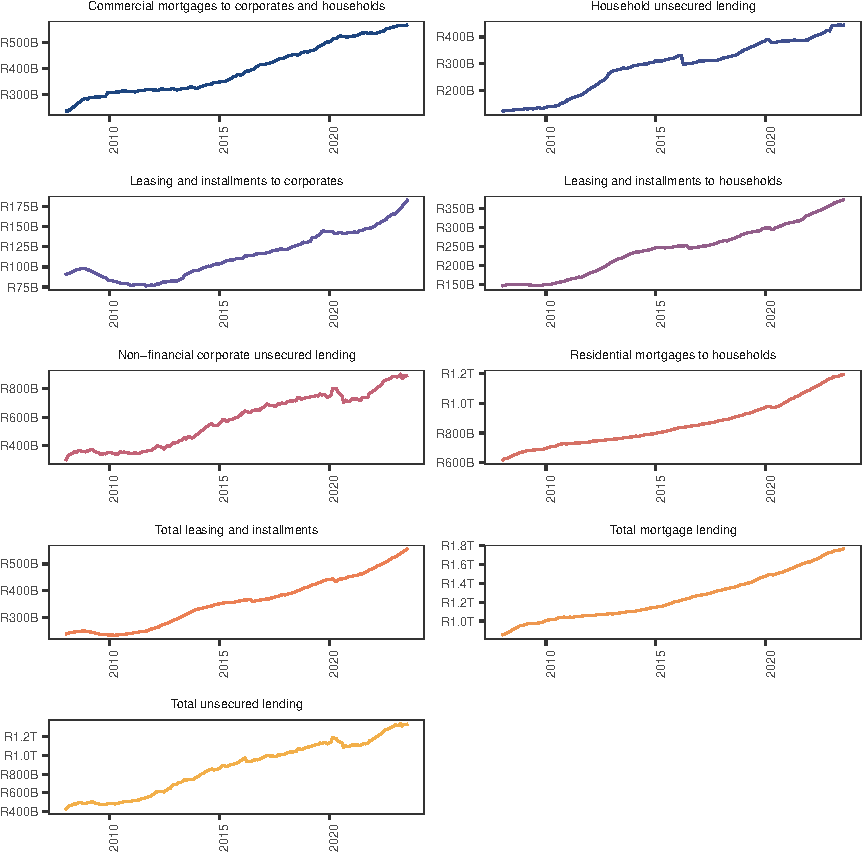
\includegraphics{UP_paper_v2_files/figure-pdf/fig-bank_lending-1.pdf}

}

\caption{\label{fig-bank_lending}Total aggregated bank lending}

\end{figure}%

\subsection{Weighted lending rates
(aggregated)}\label{weighted-lending-rates-aggregated}

\begin{figure}[H]

\centering{

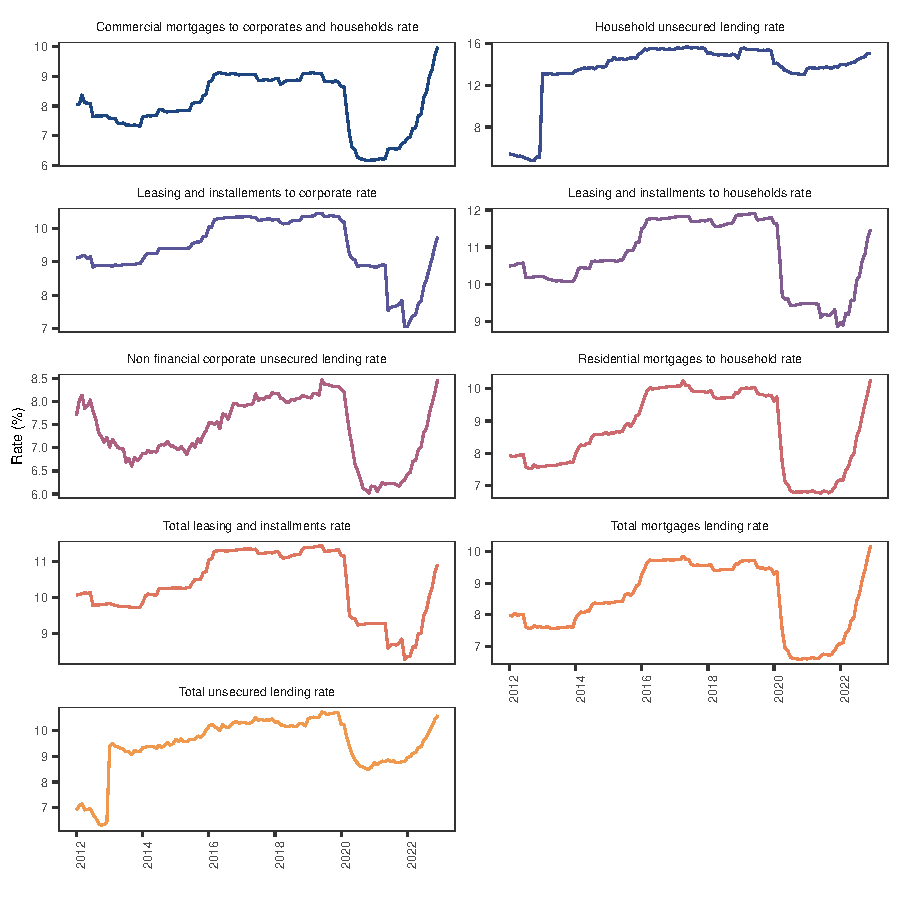
\includegraphics{UP_paper_v2_files/figure-pdf/fig-bank_interest_rates-1.pdf}

}

\caption{\label{fig-bank_interest_rates}Weighted lending rates}

\end{figure}%

\newpage

\subsection{Description of narrative
events}\label{description-of-narrative-events}

\subsubsection{Macroprudential
Indicators}\label{macroprudential-indicators}

This section provides a detailed account of the narrative
macroprudential indicators. The asterisk (*) indicates that the specific
regulation is tracked from the date of announcement to the date of
implementation.

2008/01/01: \textcolor{ForestGreen}{Implementation}

\begin{quote}
            BASEL II is  Implemented until Dec 2011
\end{quote}

2009/02/04:
\textcolor{blue}{Announcement, draft and passing of regulation}

\begin{quote}SARB issues  \textbf{directive 1/2009 (1 of 2009)} announcing the approach banks should follow in the application of capital floors. "Modelled capital should not be below 80\% of the capital requirements under Basel I to ensure capital levels do not fall below prudent level". Following Basel II, banks are allowed to use internal models to determine risk weights and in turn, determine capital levels. However, capital floors ensure capital requirements did not fall below a certain percentage of banks’ capital requirements under the previous Basel I framework\citep{basel06}. This in essence, imply greater risk weight attached to riskier credit products. For instance,  \cite{imbierowicz2018time} show that Danish banks reducing their lending on loans with higher risk weights, in response to higher capital requirements, including approaches to capital floors.
 \end{quote}

2009/07/31*:
\textcolor{blue}{Announcement, draft and passing of regulation}

\begin{quote}BCBS announces "measures to strengthen the 1996 rules governing trading book capital and to enhance the three pillars of the Basel II framework (Basel 2.5)". This in essence, aims  to introduce higher capital requirements to capture the credit risk of complex trading activities, promote the build-up of capital buffers that can be drawn down in periods of stress and strengthen the quality of bank capital\citep{basel09}
                \end{quote}

2010/10/08*:
\textcolor{blue}{Announcement, draft and passing of regulation}

\begin{quote}SARB issues \textbf{circular 3/2010} endorsing and giving notices to banks to prepare for the implementation of Basel 2.5, following the communication by the BCBS on July 31, 2009

\end{quote}

2011/06/30*:
\textcolor{blue}{Announcement, draft and passing of regulation}

\begin{quote}BCBS issues and publishes Basel III: A Global Regulatory Framework for More Resilient Banks and Banking Systems. 
\end{quote}

2011/07/31:
\textcolor{blue}{Announcement, draft and passing of regulation}

\begin{quote} 
Cabinet adopts proposal to shift to Twin Peaks Model of Financial Regulation in South Africa, following he GFC, with the aim of improving  institutional structure to support financial regulation. This is a signal to stricter oversight on the overall financial system
\end{quote}

2011/10/31:
\textcolor{blue}{Announcement, draft and passing of regulation}

\begin{quote}
    Basel 2.5 is transposed into domestic law (next step is implementation)
\end{quote}

2012/01/01: \textcolor{ForestGreen}{Implementation}

\begin{quote}
    Basel 2.5 takes effect: SARB minimum capital requirements
    \begin{itemize}
        \item Total CET1, 5.25\%, Total Tier1, 7\%, Minimum regulatory capital, 8\%, Total regulatory capital for D-SIB, 9.5\%
    \end{itemize}
\end{quote}

2012/02/16*:
\textcolor{blue}{Announcement, draft and passing of regulation}

\begin{quote}
    
SARB issues \textbf{guidance note 2/2012} announcing on new definition of total regulatory capital for Basel III such as:
\begin{itemize}
    \item Phasing out arrangements for non-common equity Tier 1 capital instruments that no longer qualify as regulatory capital under Basel III
 \item Transitional arrangements for Basel III implementation
\item Treatment of disclosed reserves under Basel III

\end{itemize}
\end{quote}

2012/05/31*:
\textcolor{blue}{Announcement, draft and passing of regulation}

\begin{quote}
SARB issues \textbf{guidance Note G5/2012} announcing that it will provide  liquidity facility to assist banks in meeting the liquidity Coverage Ratio (LCR) and cash reserves can be included as banks' high quality liquid assets for calculating LCR. This follows results from Quantitative Impact Studies (QIS) exercises by banks,  which revealed some banks would have shortfalls of around R140 billion in meeting the 100\% LCR  by 1 Jan 2019 due do to reliance eon short-term funding limited availability of HQLA

\begin{itemize}
    \item LCR requirements will be introduced on \textbf{1 Jan 2015} at 60\%, increasing by 10\% to reach 100\% on 1 Jan 2019
\item Level 1 assets (stocks, funds or bonds) shall comprise 60\% of total HQLA  while level 2 assets (less liquid) shall constitute no more than the remaining 40\%
\item SARB proposes that Leverage ratio be set at 4\% (LR of 4\% implies that banks' leverage does not exceed its capital by 40\%)
\end{itemize}

\end{quote}

2012/08/15*:
\textcolor{blue}{Announcement, draft and passing of regulation}

\begin{quote}
SARB transposes Basel III into law and publishes Counter-cyclical Capital Buffer (CCyB) rules, set to be implemented on 1 January 2016
\end{quote}

2013/01/31/*: \textcolor{ForestGreen}{Implementation}

\begin{quote}
    Basel III takes effect
\end{quote}

2013/08/20:
\textcolor{blue}{Announcement, draft and passing of regulation}

\begin{quote}
 SARB issues \textbf{Guidance Note 6/2013} announcing that banks' cash reserves may be included as part of their level 1 HQLA. Only equities listed on JSE's main exchange and included on Top 40 Index shall be considered as level2 HQLA (\textit{Potentially limit banks' ability to raise capital}).
\end{quote}

2014/01/31: \textcolor{ForestGreen}{Implementation}

\begin{quote}
SARB mimimum Capital Requirements increase to:\\
Total CET1, 5,5\%, Total Tier1, 7\%, Total regulatory capital, 8\%, Total regulatory capital for D-SIB, 10\%
\end{quote}

2014/12/31:
\textcolor{blue}{Announcement, draft and passing of regulation}

\begin{quote}
SARB issues \textbf{guidance note 8/2014} announcing  the provision of a committed liquidity facility  (CLF). This is to assist banks to meet the LCR.
Banks, however need to have collateral to access the CLF, consisting of:
\begin{itemize}
    \item  High-quality residential mortgage loans
\item Other loans and advances such as VAF, excluding unsecured loans
\item Domestically listed securities
\end{itemize}
\end{quote}

2015/01/31*: \textcolor{ForestGreen}{Implementation}

\begin{quote}
LCR ratio is introduced/implemented at 60\% compliance
\end{quote}

2015/12/31*:
\textcolor{blue}{Announcement, draft and passing of regulation}

\begin{quote}
SARB issues \textbf{circular 8/2015} announcing timelines and targets in respect of  the implementation of the countercyclical capital buffer (CCyB). SARB requirements shall apply to bank-wide total RWA:
\begin{itemize}
    \item 0.625\% on 1 Jan 2016
\item 1.25\% 1 Jan 2017
\item 1.875\% on 1 Jan 2018
\item 2.5\% on 1 Jan 2019
\end{itemize}
\end{quote}

2016/01/31*: \textcolor{ForestGreen}{Implementation}

\begin{quote}
CCyB is implemented and set at 0.625\% 
\end{quote}

2016/04/13*:
\textcolor{blue}{Announcement, draft and passing of regulation}

\begin{quote}
SARB issues \textbf{directive 1/2016} to inform all banks of matters related to the exposure limits imposed in the classification of deposits and credit exposures to small and medium enterprises  (SMEs), to be implemented on 1 July 2016. For instance, total exposure of a bank to an SME borrower, which shall be determined or calculated on a consolidated basis, at no time exceeds R12,5 million (\textit{Greater limits on value of a loan that can be extended to an SME})
\end{quote}

2016/07/01*: \textcolor{ForestGreen}{Implementation}

\begin{quote}
Exposure limits imposed in the classification of deposits and credit exposures to small and medium enterprises  (SMEs), announced on 2016/04/13, is implemented
\end{quote}

2017/01/31*: \textcolor{ForestGreen}{Implementation}

\begin{quote}
LCR ratio is introduced/implemented at 80\% compliance, while CCyB increases to 1.25\%
\end{quote}

\begin{quote}
2017/12/13*: \textcolor{blue}{Announcement, draft and passing of regulation}
SARB issues \textbf{directive 8/2017} informing banks to comply with the Net Stable Funding Ratio (NSFR) framework and on matters related to calibration of NSFR, including  template to monitor NSFR compliance. Agrees to start implementation on 1 January 2018. Objective is to reduce funding risk over a longer time horizon by requiring banks to fund their activities with sufficiently stable sources of funding in order to mitigate the risk of future funding stress. \textit{Banks will be required to match their funding with their outflows, which may lead to a greater demand for longer term funding. Longer term funding will result in an increased cost of funding for banks (possibly passed on to borrowers and lower profitability and returns for banks}
\end{quote}

2018/01/31*: \textcolor{ForestGreen}{Implementation}

\begin{quote}
NSFR Implemented following  Directive 8/2017, CCyB increases to 1,875\% and LCR is implemented at 90\% compliance.
\end{quote}

2019/01/31*: \textcolor{ForestGreen}{Implementation}

\begin{quote}
CCyB increases to 2,5\% (maximum) and LCR is implemented at 100\% compliance.
\end{quote}

\newpage

\subsubsection{Finance regulation index}\label{finance-regulation-index}

\textbf{Changes in the National Credit Act of 2005 Regulations}

The National Credit Act of 2005 is legislation that was enacted in order
to better regulate the markets for customer credit. According to this
Act its purpose is to develop, inter alia, credit markets that are
accessible by all South Africans, correct the imbalance in negotiating
power between consumers and credit providers, regulate the collection
and sharing of consumer credit information and prevent
over-indebtedness. These, and other, efforts are to achieve a
\emph{``fair, transparent, competitive, sustainable, responsible,
efficient, effective and accessible credit market and industry, and to
protect consumers}\^{} {[}Section 3 of the NCA.{]}. The Act specifically
provided the Minister of, the erstwhile, Trade and Industry with powers
to provide regulations pertaining to the implementation of the
Act.\footnote{Section 171 of the NCA.} These regulations were made
available in May 2006.

The initial regulations predate the period assessed by this paper, but
the proposed and later realised changes to these Regulations occurred
between 2012 and 2015. It is these developments that are captured within
\(FinReg\).

\emph{2012 Debt Counselling Regulations}

On the 10th of May 2012 the Minister of Trade and Industry published
debt counselling regulations. These codified the process to be followed
by debt counselors and consumers when seeking various order from the
Magistrate's Court. These orders relate to the re-structuring of debt
following a debt counselor's findings of consumer over-indebtedness,
consumer difficulty to meet debt obligations and direct applications by
consumers to the court following an adverse finding by debt counsellors.
The regulations also provided that credit providers were expected to
implement orders from the Court within 10 working days following their
receipt of the court orders from the debt counselors and/or consumers
\citep{regulations2012}.\footnote{The initial draft regulations were
  published on the 15th of May 2009 and did not prescribe the period
  within which court orders, made following debt counselling processes,
  were to be implemented by credit providers}.

\citet{Roestoff2009} indicates that provisions of the National Credit
Act in regard to debt relief are to assist over-indebted consumers,
prioritising their interests more than those of credit providers. To
achieve these outcomes, debt review negotiations require that credit
providers have greater responsibility toward the possible negative
outcomes of credit provision.

\emph{2013 and 2014 draft and final credit regulations on the removal of
adverse consumer credit information and information relating to paid up
judgements}

In 2013 the Minister of Trade and Industry issued a notice about a
proposal to remove adverse credit information from credit bureaus. This
followed Cabinet endorsement of a \emph{Removal of Adverse Credit
Information Project}. The Minister proposed that all adverse findings
were to be removed regardless of non-payment. Thereafter on an ongoing
basis adverse information held by credit bureaus were on settled debt or
paid up judgements were to be removed. Communication from the SA
government indicated that this move was to ensure that those who could
access credit, and were prevented from doing so, due to adverse credit
information could do so \citep{gcis2013}.

On the 26th of February 2014, the Minister published final regulations
instructing credit bureaus that adverse credit information was to be
removed on all paid up judgements \citep{regulations2014a}. The final
regulations were less ambitious than the proposal. Nevertheless, the
\citet{ncrnd} indicates that the regulations were to enable consumer
access to affordable credit, as well as employment opportunities
\citet{ncrnd}

\emph{2014 and 2015 changes to the National Credit Regulations}

On the 1st of August 2014, the Minister of Trade and Industry published
draft national credit regulations that proposed a host of changes to the
existing 2006 regulations, as amended \citep{regulations2014b}. Many of
these were proposed insertions into the regulations that did not exist
before. The proposals included a criteria to be adopted by credit
providers to conduct affordability assessments to further limit
instances of reckless lending. Credit providers were provided with
additional limits on when adverse consumer credit information was to be
shared with credit bureaus; for instance, information that consumers did
not meet their financial obligations would not be shared unless a
consumer would have missed their minimum obligations for three
consecutive months. Related to credit bureau information were changes to
the maximum periods that credit information were to be kept by credit
bureaus. For many of the types of information kept, the proposed
regulations proposed reduced retention periods. For instance,
information relating to enquiries on a consumers record was to be
reduced from 2 years to 2 months; information on liquidations had been
kept for an unlimited period and the proposal was to reduce this to 5
years; information on complaints initiated by customers was kept from 18
months and proposed to be reduced to 6 months. Other changes included
explicit references to the registration and operation of payment
distribution agents, as well as the provision of clarity on when credit
information could be obtained for employment purposes.

By the 13th of March 2015, the Minister provided a final set of proposed
changes and insertions into the regulations that would come into effect
\citep{regulations2015a}. Many of the 2014 proposals were accepted, some
with changes. Some of these included the explicit criteria for
affordability assessments, changes to the retention periods for credit
bureau information, and the additional limits on when adverse consumer
credit information was to be shared with credit bureaus.

\emph{2015 draft and final credit regulations on limitations on fees and
interest rates}

Section 42(1) of the 2006 credit regulations provided the maximum
interest rates to be set on different types of
credit\citep{regulations2006}. These included mortgages, credit
facilities, unsecured credit, developmental credit, short term credit,
other and incidental credit agreements. Incidental and short term credit
rates were respectively capped at 2\% and 5\% per month. The limits for
other rates were calculated at the repo rate scaled up by 2.2 and
increased by fixed interest rates ranging between 5 to 20 percentage
points depending on the credit type. In addition, the regulations also
provided the maximum Rand values that would be set as initiation and
service fees. The initiation fees varied by credit type.

In 2015, the Minister of Trade and Industry proposed changes to these
interest rates and initiation fees \citep{regulations2015b}. Final
changes came into effects that same year \citep{regulations2015c}. For 5
of the 7 credit types, the Minister provided a lower scalar by higher
interest rate premium. The net effect of this adjustment was that
maximum interest rates on credit facilities would be lower by 2.9
percentage points and 7.9 percentage points for unsecured credit (based
on the prevailing repo rate). The maximum rates set for other credit
types increased marginally by 0.1 percentage points of had no change at
all. Initiation and service fees were increased above the limits set in
the 2006 regulations.

\textbf{Restructuring of the financial sector regulation}

\emph{Financial Sector Regulation Act}

The Financial Sector Regulation Act of 2017 represented a structural
shift in the regulation of financial institutions in South Africa, as it
set up a framework for financial regulation and supervision.

The Act importantly sets up two authorities with important regulatory
powers. One is the Prudential Authority, which sits within the South
African Reserve Bank. This object of this authority is to ensure the
soundness of financial institutions and infrastructure and financial
stability, as well as protecting consumers against risks from financial
institutions. The other authority created by the act is the Financial
Sector Conduct Authority (FSCA).\footnote{The FSCA replaced the
  Financial Services Board. See:
  https://www.fsca.co.za/TPNL/4/fsb4/proactive.html} The object of the
FSCA was to protect financial consumers by promoting fair treatment and
financial education, as well as to maintaining financial stability and
market efficiency.

Both the PA and the FSCA were tasked with promoting financial inclusion.
Which the Act defined as a state where all persons have access to
\emph{``timely and fair access to appropriate, fair and affordable
financial products and services''} \citep{fsr2017}.

\emph{Draft and Update of the Conduct of Financial Institutions Bill}

In 2018 the National Treasury presented a draft Conduct of Financial
Institutions (COFI) Bill. This bill proposes consolidating a number of
the financial sector laws of the country. At present, the nature of
financial sector regulation is focused on particular sectors. For
instance, insurance companies are regulated by the Insurance Act,
investment schemes by the Collective Investment Schemes Control Act and
financial service providers by the Financial Advisory and Intermediary
Services Act. The proposed bill seeks to provide the provide the
Financial Services Conduct Authority with the ability to regulate the
conduct of institution that provide the similar services and products
\citep{cofi2018a}.

With regard to credit provision, the COFI bill proposes providing the
FSCA with the ability to provide standards for the conduct of firms in
the provision of financial products and services. The referred to
conduct relates to, inter alia, firms' charging structures, pricing
methodologies, financial product features and the identification of
appropriate and inappropriate target markets
\citep[\citet{cofi2020}]{cofi2018a}. The \citet{cofi2018b} explains that
this proposed legislation is premised on supporting greater financial
inclusion as the better regulation of firm conduct would provide
consumers with greater security required for their usage of financial
sector products. A draft COFI bill was presented in 2018 and an updated
draft in 2020 \citep{cofi2020}.

\textbf{National financial inclusion policy}

\emph{Draft Financial Inclusion Policy Report is published}

In 2020 the National Treasury provided a draft national policy framework
for financial inclusion in South Africa. The existing state of financial
inclusion is reported to be high in South Africa but the National
Treasury notes that the usage of financial products by low income
earners remains low and that small, medium and micro enterprises are
only marginally serviced \citep{nt2020}. On the back of these
challenges, the draft national policy framework provides the initiatives
to be support the three key pillars they identify as being important to
financial inclusion: (i) deepening financial inclusion, (ii) improving
access for SMMEs and (iii) supporting more diverse providers of
financial services.

A number of initiatives identified by the \citet{nt2020} in the above
mentioned three pillars relate directly to credit currently extended by
incumbent banks. To increase developmental loans provided to low income
families, the policy proposes governments sharing losses on defaults and
a students future income to assess affordability of loans, as well as
the use of different forms of collateral (such as a permission to
occupy) to secure mortgage financing. SMME access to financing is
planned to be supported by improvements in credit infrastructure for
small businesses; an example of this will include consideration of SMME
payments data as information relevant to determining ability to access
credit. To support more providers of financial services \citet{nt2020}
proposes promoting the development of cooperative banks to compete
against incumbent banks, developing a licensing framework that supports
the entry of new financial institutions and assessing the role of a
state owned bank.

The financial inclusion policy sets out a number of initiatives that are
likely to have an impact when and how incumbent banks extend credit. In
addition, the proposed framework as suggests various programmes that
would create additional financial institutions that are likely to
compete with incumbents in markets relating to credit provision.

\subsection{Macroprudential narrative
indexes}\label{macroprudential-narrative-indexes}

\begin{figure}[H]

\centering{

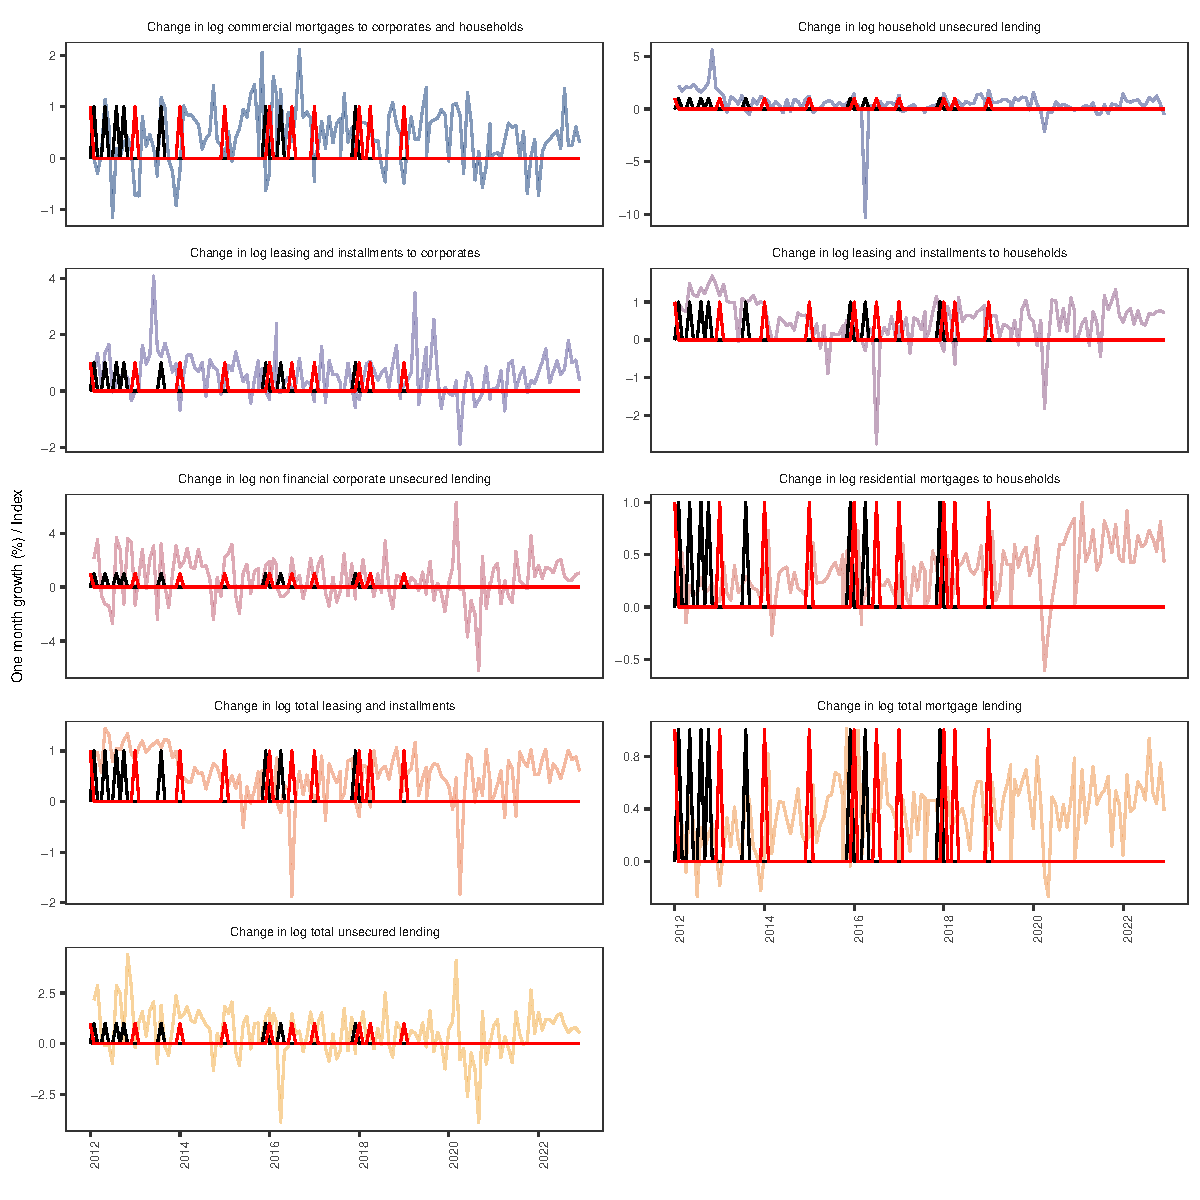
\includegraphics{UP_paper_v2_files/figure-pdf/fig-macro_narrative_indexes_one_month-1.pdf}

}

\caption{\label{fig-macro_narrative_indexes_one_month}One month lending
growth and macroprudential narrative index comparison. Note: The black
line represents the Draft index, and the red line represents the
Implementation index.}

\end{figure}%

\newpage

\begin{figure}[H]

\centering{

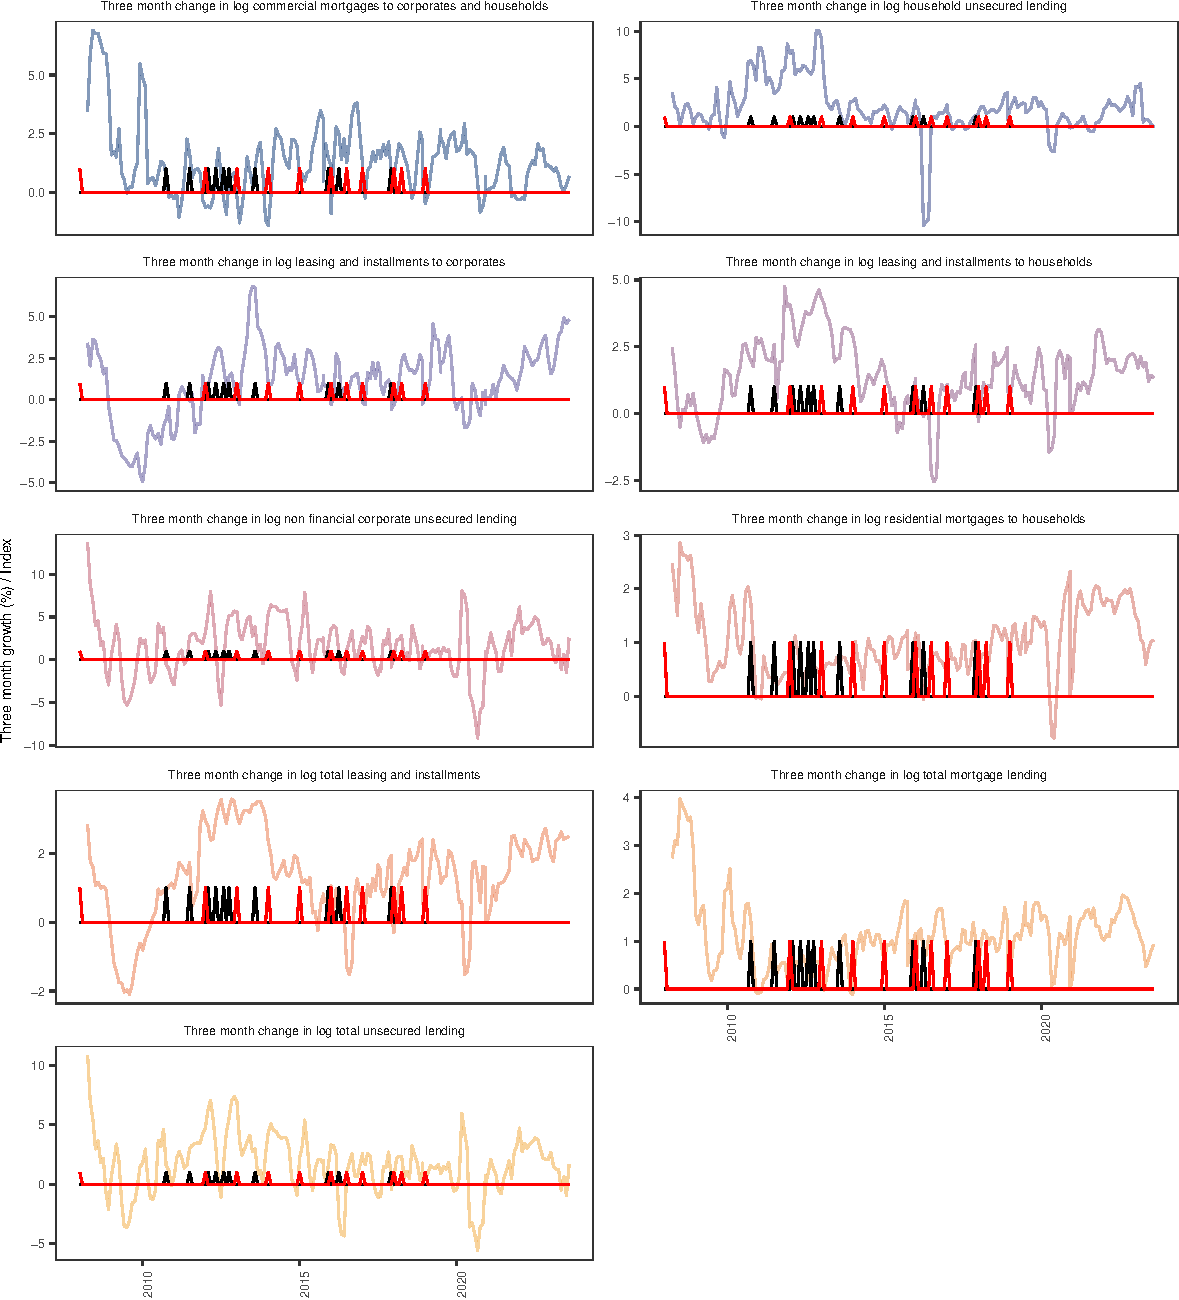
\includegraphics{UP_paper_v2_files/figure-pdf/fig-macro_narrative_indexes_three_month-1.pdf}

}

\caption{\label{fig-macro_narrative_indexes_three_month}Three month
lending growth and macroprudential narrative indexes comparison. Note:
The black line represents the Draft index, and the red line represents
the Implementation index.}

\end{figure}%

\newpage

\subsection{Financial regulation narrative
indexes}\label{financial-regulation-narrative-indexes}

\begin{figure}[H]

\centering{

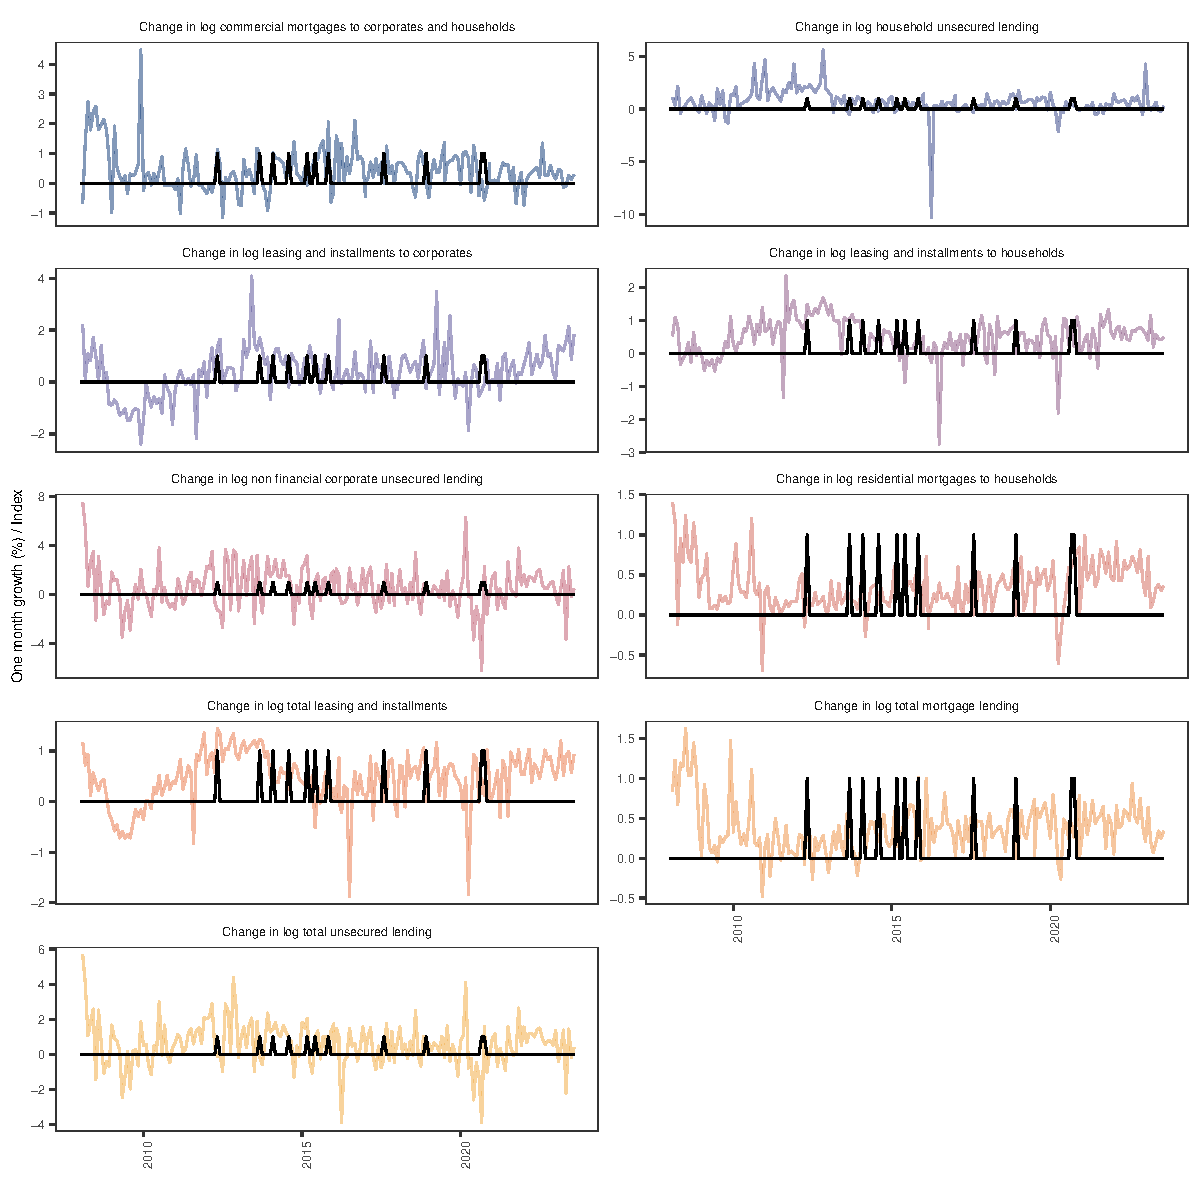
\includegraphics{UP_paper_v2_files/figure-pdf/fig-comp_narrative_indexes_one_month-1.pdf}

}

\caption{\label{fig-comp_narrative_indexes_one_month}One month lending
growth and financial narrative index comparison. Note: The black line
represents the Financial regulation index.}

\end{figure}%

\newpage

\begin{figure}[H]

\centering{

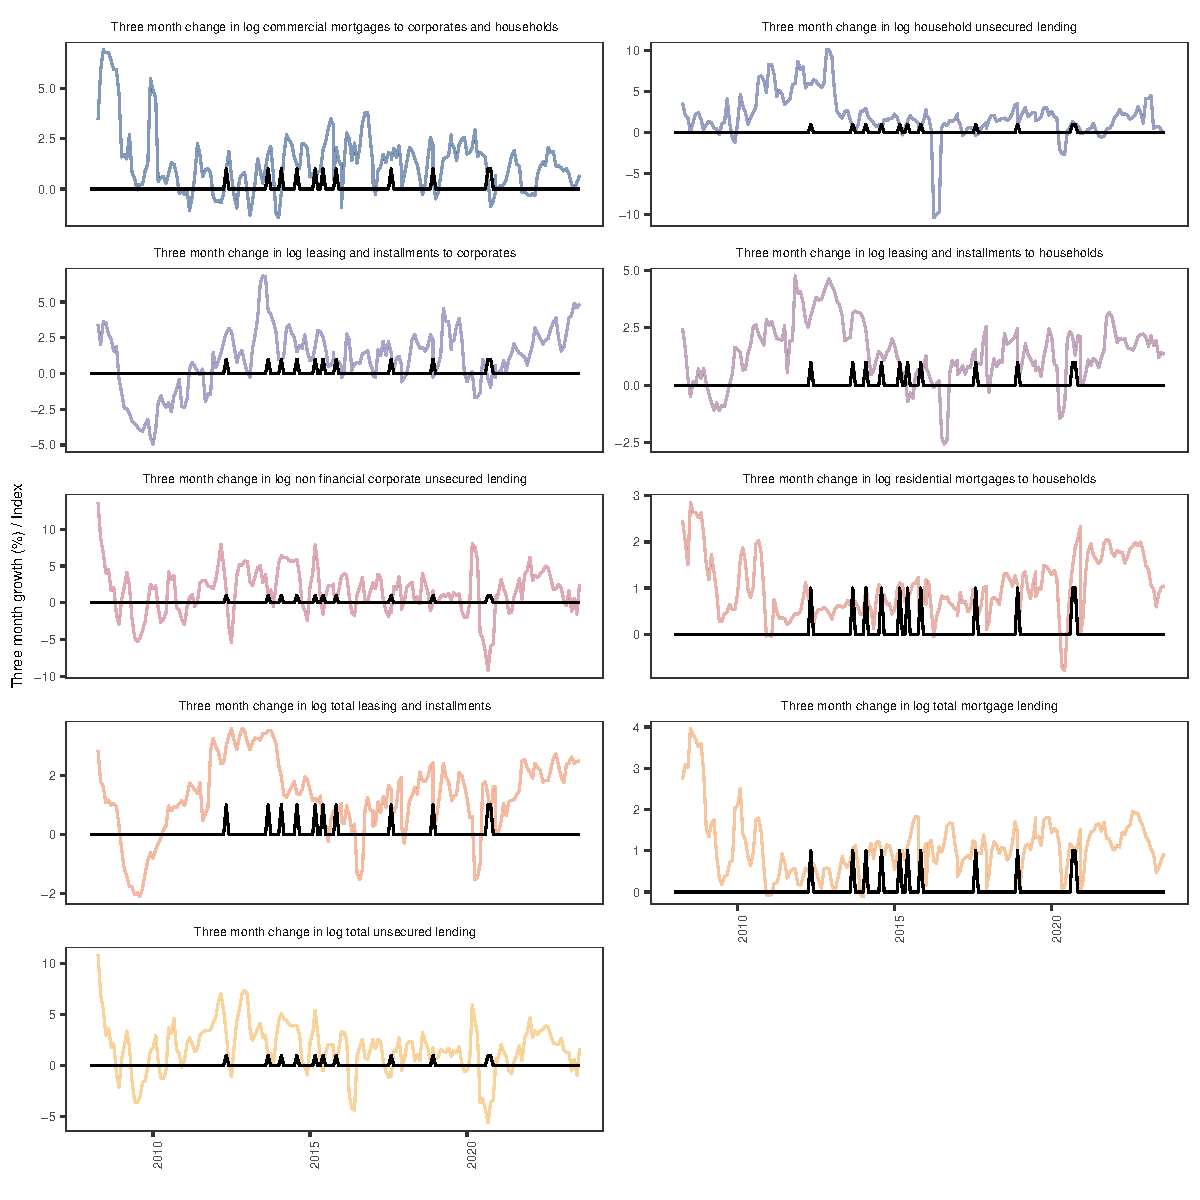
\includegraphics{UP_paper_v2_files/figure-pdf/fig-comp_narrative_indexes_three_month-1.pdf}

}

\caption{\label{fig-comp_narrative_indexes_three_month}Three month
lending growth and financial narrative indexes comparison. Note: The
black line represents the Financial regulation index.}

\end{figure}%

\newpage

\bsideways

\subsection{Results with controls}\label{results-with-controls}

\global\setlength{\Oldarrayrulewidth}{\arrayrulewidth}

\global\setlength{\Oldtabcolsep}{\tabcolsep}

\setlength{\tabcolsep}{2pt}

\renewcommand*{\arraystretch}{1}



\providecommand{\ascline}[3]{\noalign{\global\arrayrulewidth #1}\arrayrulecolor[HTML]{#2}\cline{#3}}

\begin{longtable}[l]{|p{1.40in}|p{0.75in}|p{0.75in}|p{0.75in}|p{0.75in}|p{0.75in}|p{0.75in}|p{0.75in}|p{0.75in}|p{0.75in}}

\caption{\label{tbl-macropru_draft_lending_control}Macroprudential
regulations and lending volumes (3-months) with controls results}

\tabularnewline

\ascline{1pt}{000000}{1-10}

\multicolumn{1}{>{\centering}m{\dimexpr 1.4in+0\tabcolsep}}{\textcolor[HTML]{000000}{\fontsize{7}{7}\selectfont{}}} & \multicolumn{3}{!{\color[HTML]{FFFFFF}\vrule width 1pt}>{\centering}m{\dimexpr 2.25in+4\tabcolsep+2pt}}{\textcolor[HTML]{000000}{\fontsize{7}{7}\selectfont{Total}}} & \multicolumn{3}{!{\color[HTML]{FFFFFF}\vrule width 1pt}>{\centering}m{\dimexpr 2.25in+4\tabcolsep+2pt}}{\textcolor[HTML]{000000}{\fontsize{7}{7}\selectfont{Corporates}}} & \multicolumn{3}{!{\color[HTML]{FFFFFF}\vrule width 1pt}>{\centering}m{\dimexpr 2.25in+4\tabcolsep+2pt}!{\color[HTML]{FFFFFF}\vrule width 1pt}}{\textcolor[HTML]{000000}{\fontsize{7}{7}\selectfont{Households}}} \\

\ascline{1pt}{FFFFFF}{1-1}\ascline{1pt}{000000}{2-10}



\multicolumn{1}{>{\raggedright}m{\dimexpr 1.4in+0\tabcolsep}}{\textcolor[HTML]{000000}{\fontsize{7}{7}\selectfont{\ }}} & \multicolumn{1}{!{\color[HTML]{FFFFFF}\vrule width 1pt}>{\raggedright}m{\dimexpr 0.75in+0\tabcolsep}}{\textcolor[HTML]{000000}{\fontsize{7}{7}\selectfont{Unsecured}}} & \multicolumn{1}{!{\color[HTML]{FFFFFF}\vrule width 1pt}>{\raggedright}m{\dimexpr 0.75in+0\tabcolsep}}{\textcolor[HTML]{000000}{\fontsize{7}{7}\selectfont{Secured}}} & \multicolumn{1}{!{\color[HTML]{FFFFFF}\vrule width 1pt}>{\raggedright}m{\dimexpr 0.75in+0\tabcolsep}}{\textcolor[HTML]{000000}{\fontsize{7}{7}\selectfont{Mortgages}}} & \multicolumn{1}{!{\color[HTML]{FFFFFF}\vrule width 1pt}>{\raggedright}m{\dimexpr 0.75in+0\tabcolsep}}{\textcolor[HTML]{000000}{\fontsize{7}{7}\selectfont{Unsecured}}} & \multicolumn{1}{!{\color[HTML]{FFFFFF}\vrule width 1pt}>{\raggedright}m{\dimexpr 0.75in+0\tabcolsep}}{\textcolor[HTML]{000000}{\fontsize{7}{7}\selectfont{Secured}}} & \multicolumn{1}{!{\color[HTML]{FFFFFF}\vrule width 1pt}>{\raggedright}m{\dimexpr 0.75in+0\tabcolsep}}{\textcolor[HTML]{000000}{\fontsize{7}{7}\selectfont{Mortgages}}} & \multicolumn{1}{!{\color[HTML]{FFFFFF}\vrule width 1pt}>{\raggedright}m{\dimexpr 0.75in+0\tabcolsep}}{\textcolor[HTML]{000000}{\fontsize{7}{7}\selectfont{Unsecured}}} & \multicolumn{1}{!{\color[HTML]{FFFFFF}\vrule width 1pt}>{\raggedright}m{\dimexpr 0.75in+0\tabcolsep}}{\textcolor[HTML]{000000}{\fontsize{7}{7}\selectfont{Secured}}} & \multicolumn{1}{!{\color[HTML]{FFFFFF}\vrule width 1pt}>{\raggedright}m{\dimexpr 0.75in+0\tabcolsep}}{\textcolor[HTML]{000000}{\fontsize{7}{7}\selectfont{Mortgages}}} \\

\ascline{1pt}{000000}{1-10}\endfirsthead 

\ascline{1pt}{000000}{1-10}

\multicolumn{1}{>{\centering}m{\dimexpr 1.4in+0\tabcolsep}}{\textcolor[HTML]{000000}{\fontsize{7}{7}\selectfont{}}} & \multicolumn{3}{!{\color[HTML]{FFFFFF}\vrule width 1pt}>{\centering}m{\dimexpr 2.25in+4\tabcolsep+2pt}}{\textcolor[HTML]{000000}{\fontsize{7}{7}\selectfont{Total}}} & \multicolumn{3}{!{\color[HTML]{FFFFFF}\vrule width 1pt}>{\centering}m{\dimexpr 2.25in+4\tabcolsep+2pt}}{\textcolor[HTML]{000000}{\fontsize{7}{7}\selectfont{Corporates}}} & \multicolumn{3}{!{\color[HTML]{FFFFFF}\vrule width 1pt}>{\centering}m{\dimexpr 2.25in+4\tabcolsep+2pt}!{\color[HTML]{FFFFFF}\vrule width 1pt}}{\textcolor[HTML]{000000}{\fontsize{7}{7}\selectfont{Households}}} \\

\ascline{1pt}{FFFFFF}{1-1}\ascline{1pt}{000000}{2-10}



\multicolumn{1}{>{\raggedright}m{\dimexpr 1.4in+0\tabcolsep}}{\textcolor[HTML]{000000}{\fontsize{7}{7}\selectfont{\ }}} & \multicolumn{1}{!{\color[HTML]{FFFFFF}\vrule width 1pt}>{\raggedright}m{\dimexpr 0.75in+0\tabcolsep}}{\textcolor[HTML]{000000}{\fontsize{7}{7}\selectfont{Unsecured}}} & \multicolumn{1}{!{\color[HTML]{FFFFFF}\vrule width 1pt}>{\raggedright}m{\dimexpr 0.75in+0\tabcolsep}}{\textcolor[HTML]{000000}{\fontsize{7}{7}\selectfont{Secured}}} & \multicolumn{1}{!{\color[HTML]{FFFFFF}\vrule width 1pt}>{\raggedright}m{\dimexpr 0.75in+0\tabcolsep}}{\textcolor[HTML]{000000}{\fontsize{7}{7}\selectfont{Mortgages}}} & \multicolumn{1}{!{\color[HTML]{FFFFFF}\vrule width 1pt}>{\raggedright}m{\dimexpr 0.75in+0\tabcolsep}}{\textcolor[HTML]{000000}{\fontsize{7}{7}\selectfont{Unsecured}}} & \multicolumn{1}{!{\color[HTML]{FFFFFF}\vrule width 1pt}>{\raggedright}m{\dimexpr 0.75in+0\tabcolsep}}{\textcolor[HTML]{000000}{\fontsize{7}{7}\selectfont{Secured}}} & \multicolumn{1}{!{\color[HTML]{FFFFFF}\vrule width 1pt}>{\raggedright}m{\dimexpr 0.75in+0\tabcolsep}}{\textcolor[HTML]{000000}{\fontsize{7}{7}\selectfont{Mortgages}}} & \multicolumn{1}{!{\color[HTML]{FFFFFF}\vrule width 1pt}>{\raggedright}m{\dimexpr 0.75in+0\tabcolsep}}{\textcolor[HTML]{000000}{\fontsize{7}{7}\selectfont{Unsecured}}} & \multicolumn{1}{!{\color[HTML]{FFFFFF}\vrule width 1pt}>{\raggedright}m{\dimexpr 0.75in+0\tabcolsep}}{\textcolor[HTML]{000000}{\fontsize{7}{7}\selectfont{Secured}}} & \multicolumn{1}{!{\color[HTML]{FFFFFF}\vrule width 1pt}>{\raggedright}m{\dimexpr 0.75in+0\tabcolsep}}{\textcolor[HTML]{000000}{\fontsize{7}{7}\selectfont{Mortgages}}} \\

\ascline{1pt}{000000}{1-10}\endhead



\multicolumn{10}{>{\centering}m{\dimexpr 8.15in+18\tabcolsep+9pt}!{\color[HTML]{FFFFFF}\vrule width 1pt}}{\textcolor[HTML]{000000}{\fontsize{7}{7}\selectfont{Draft\ model}}} \\

\ascline{1pt}{FFFFFF}{1-10}



\multicolumn{1}{>{\raggedright}m{\dimexpr 1.4in+0\tabcolsep}}{\textcolor[HTML]{000000}{\fontsize{7}{7}\selectfont{Draft\ index}}} & \multicolumn{1}{!{\color[HTML]{FFFFFF}\vrule width 1pt}>{\raggedright}m{\dimexpr 0.75in+0\tabcolsep}}{\textcolor[HTML]{000000}{\fontsize{7}{7}\selectfont{0.641}}} & \multicolumn{1}{!{\color[HTML]{FFFFFF}\vrule width 1pt}>{\raggedright}m{\dimexpr 0.75in+0\tabcolsep}}{\textcolor[HTML]{000000}{\fontsize{7}{7}\selectfont{2.279**}}} & \multicolumn{1}{!{\color[HTML]{FFFFFF}\vrule width 1pt}>{\raggedright}m{\dimexpr 0.75in+0\tabcolsep}}{\textcolor[HTML]{000000}{\fontsize{7}{7}\selectfont{-0.186**}}} & \multicolumn{1}{!{\color[HTML]{FFFFFF}\vrule width 1pt}>{\raggedright}m{\dimexpr 0.75in+0\tabcolsep}}{\textcolor[HTML]{000000}{\fontsize{7}{7}\selectfont{0.423}}} & \multicolumn{1}{!{\color[HTML]{FFFFFF}\vrule width 1pt}>{\raggedright}m{\dimexpr 0.75in+0\tabcolsep}}{\textcolor[HTML]{000000}{\fontsize{7}{7}\selectfont{0.891***}}} & \multicolumn{1}{!{\color[HTML]{FFFFFF}\vrule width 1pt}>{\raggedright}m{\dimexpr 0.75in+0\tabcolsep}}{\textcolor[HTML]{000000}{\fontsize{7}{7}\selectfont{-0.375}}} & \multicolumn{1}{!{\color[HTML]{FFFFFF}\vrule width 1pt}>{\raggedright}m{\dimexpr 0.75in+0\tabcolsep}}{\textcolor[HTML]{000000}{\fontsize{7}{7}\selectfont{1.035**}}} & \multicolumn{1}{!{\color[HTML]{FFFFFF}\vrule width 1pt}>{\raggedright}m{\dimexpr 0.75in+0\tabcolsep}}{\textcolor[HTML]{000000}{\fontsize{7}{7}\selectfont{3.183**}}} & \multicolumn{1}{!{\color[HTML]{FFFFFF}\vrule width 1pt}>{\raggedright}m{\dimexpr 0.75in+0\tabcolsep}}{\textcolor[HTML]{000000}{\fontsize{7}{7}\selectfont{-0.154}}} \\

\ascline{1pt}{FFFFFF}{1-10}



\multicolumn{1}{>{\raggedright}m{\dimexpr 1.4in+0\tabcolsep}}{\textcolor[HTML]{000000}{\fontsize{7}{7}\selectfont{Return\ on\ assets}}} & \multicolumn{1}{!{\color[HTML]{FFFFFF}\vrule width 1pt}>{\raggedright}m{\dimexpr 0.75in+0\tabcolsep}}{\textcolor[HTML]{000000}{\fontsize{7}{7}\selectfont{1.050}}} & \multicolumn{1}{!{\color[HTML]{FFFFFF}\vrule width 1pt}>{\raggedright}m{\dimexpr 0.75in+0\tabcolsep}}{\textcolor[HTML]{000000}{\fontsize{7}{7}\selectfont{-4.139}}} & \multicolumn{1}{!{\color[HTML]{FFFFFF}\vrule width 1pt}>{\raggedright}m{\dimexpr 0.75in+0\tabcolsep}}{\textcolor[HTML]{000000}{\fontsize{7}{7}\selectfont{-0.867}}} & \multicolumn{1}{!{\color[HTML]{FFFFFF}\vrule width 1pt}>{\raggedright}m{\dimexpr 0.75in+0\tabcolsep}}{\textcolor[HTML]{000000}{\fontsize{7}{7}\selectfont{1.497}}} & \multicolumn{1}{!{\color[HTML]{FFFFFF}\vrule width 1pt}>{\raggedright}m{\dimexpr 0.75in+0\tabcolsep}}{\textcolor[HTML]{000000}{\fontsize{7}{7}\selectfont{2.504**}}} & \multicolumn{1}{!{\color[HTML]{FFFFFF}\vrule width 1pt}>{\raggedright}m{\dimexpr 0.75in+0\tabcolsep}}{\textcolor[HTML]{000000}{\fontsize{7}{7}\selectfont{-2.102}}} & \multicolumn{1}{!{\color[HTML]{FFFFFF}\vrule width 1pt}>{\raggedright}m{\dimexpr 0.75in+0\tabcolsep}}{\textcolor[HTML]{000000}{\fontsize{7}{7}\selectfont{-0.613}}} & \multicolumn{1}{!{\color[HTML]{FFFFFF}\vrule width 1pt}>{\raggedright}m{\dimexpr 0.75in+0\tabcolsep}}{\textcolor[HTML]{000000}{\fontsize{7}{7}\selectfont{-7.865}}} & \multicolumn{1}{!{\color[HTML]{FFFFFF}\vrule width 1pt}>{\raggedright}m{\dimexpr 0.75in+0\tabcolsep}}{\textcolor[HTML]{000000}{\fontsize{7}{7}\selectfont{-0.332}}} \\

\ascline{1pt}{FFFFFF}{1-10}



\multicolumn{1}{>{\raggedright}m{\dimexpr 1.4in+0\tabcolsep}}{\textcolor[HTML]{000000}{\fontsize{7}{7}\selectfont{Total\ capital\ adequacy\ ratio}}} & \multicolumn{1}{!{\color[HTML]{FFFFFF}\vrule width 1pt}>{\raggedright}m{\dimexpr 0.75in+0\tabcolsep}}{\textcolor[HTML]{000000}{\fontsize{7}{7}\selectfont{0.233}}} & \multicolumn{1}{!{\color[HTML]{FFFFFF}\vrule width 1pt}>{\raggedright}m{\dimexpr 0.75in+0\tabcolsep}}{\textcolor[HTML]{000000}{\fontsize{7}{7}\selectfont{0.278}}} & \multicolumn{1}{!{\color[HTML]{FFFFFF}\vrule width 1pt}>{\raggedright}m{\dimexpr 0.75in+0\tabcolsep}}{\textcolor[HTML]{000000}{\fontsize{7}{7}\selectfont{0.035}}} & \multicolumn{1}{!{\color[HTML]{FFFFFF}\vrule width 1pt}>{\raggedright}m{\dimexpr 0.75in+0\tabcolsep}}{\textcolor[HTML]{000000}{\fontsize{7}{7}\selectfont{0.185}}} & \multicolumn{1}{!{\color[HTML]{FFFFFF}\vrule width 1pt}>{\raggedright}m{\dimexpr 0.75in+0\tabcolsep}}{\textcolor[HTML]{000000}{\fontsize{7}{7}\selectfont{0.141}}} & \multicolumn{1}{!{\color[HTML]{FFFFFF}\vrule width 1pt}>{\raggedright}m{\dimexpr 0.75in+0\tabcolsep}}{\textcolor[HTML]{000000}{\fontsize{7}{7}\selectfont{0.201}}} & \multicolumn{1}{!{\color[HTML]{FFFFFF}\vrule width 1pt}>{\raggedright}m{\dimexpr 0.75in+0\tabcolsep}}{\textcolor[HTML]{000000}{\fontsize{7}{7}\selectfont{0.352}}} & \multicolumn{1}{!{\color[HTML]{FFFFFF}\vrule width 1pt}>{\raggedright}m{\dimexpr 0.75in+0\tabcolsep}}{\textcolor[HTML]{000000}{\fontsize{7}{7}\selectfont{0.362}}} & \multicolumn{1}{!{\color[HTML]{FFFFFF}\vrule width 1pt}>{\raggedright}m{\dimexpr 0.75in+0\tabcolsep}}{\textcolor[HTML]{000000}{\fontsize{7}{7}\selectfont{0.001}}} \\

\ascline{1pt}{FFFFFF}{1-10}



\multicolumn{10}{>{\centering}m{\dimexpr 8.15in+18\tabcolsep+9pt}!{\color[HTML]{FFFFFF}\vrule width 1pt}}{\textcolor[HTML]{000000}{\fontsize{7}{7}\selectfont{Implementation\ model}}} \\

\ascline{1pt}{FFFFFF}{1-10}



\multicolumn{1}{>{\raggedright}m{\dimexpr 1.4in+0\tabcolsep}}{\textcolor[HTML]{000000}{\fontsize{7}{7}\selectfont{Implementation\ index}}} & \multicolumn{1}{!{\color[HTML]{FFFFFF}\vrule width 1pt}>{\raggedright}m{\dimexpr 0.75in+0\tabcolsep}}{\textcolor[HTML]{000000}{\fontsize{7}{7}\selectfont{1.52***}}} & \multicolumn{1}{!{\color[HTML]{FFFFFF}\vrule width 1pt}>{\raggedright}m{\dimexpr 0.75in+0\tabcolsep}}{\textcolor[HTML]{000000}{\fontsize{7}{7}\selectfont{1.19}}} & \multicolumn{1}{!{\color[HTML]{FFFFFF}\vrule width 1pt}>{\raggedright}m{\dimexpr 0.75in+0\tabcolsep}}{\textcolor[HTML]{000000}{\fontsize{7}{7}\selectfont{-0.49**}}} & \multicolumn{1}{!{\color[HTML]{FFFFFF}\vrule width 1pt}>{\raggedright}m{\dimexpr 0.75in+0\tabcolsep}}{\textcolor[HTML]{000000}{\fontsize{7}{7}\selectfont{1.98***}}} & \multicolumn{1}{!{\color[HTML]{FFFFFF}\vrule width 1pt}>{\raggedright}m{\dimexpr 0.75in+0\tabcolsep}}{\textcolor[HTML]{000000}{\fontsize{7}{7}\selectfont{0.69}}} & \multicolumn{1}{!{\color[HTML]{FFFFFF}\vrule width 1pt}>{\raggedright}m{\dimexpr 0.75in+0\tabcolsep}}{\textcolor[HTML]{000000}{\fontsize{7}{7}\selectfont{-1.18**}}} & \multicolumn{1}{!{\color[HTML]{FFFFFF}\vrule width 1pt}>{\raggedright}m{\dimexpr 0.75in+0\tabcolsep}}{\textcolor[HTML]{000000}{\fontsize{7}{7}\selectfont{0.55}}} & \multicolumn{1}{!{\color[HTML]{FFFFFF}\vrule width 1pt}>{\raggedright}m{\dimexpr 0.75in+0\tabcolsep}}{\textcolor[HTML]{000000}{\fontsize{7}{7}\selectfont{1.29}}} & \multicolumn{1}{!{\color[HTML]{FFFFFF}\vrule width 1pt}>{\raggedright}m{\dimexpr 0.75in+0\tabcolsep}}{\textcolor[HTML]{000000}{\fontsize{7}{7}\selectfont{-0.21*}}} \\

\ascline{1pt}{FFFFFF}{1-10}



\multicolumn{1}{>{\raggedright}m{\dimexpr 1.4in+0\tabcolsep}}{\textcolor[HTML]{000000}{\fontsize{7}{7}\selectfont{Return\ on\ assets}}} & \multicolumn{1}{!{\color[HTML]{FFFFFF}\vrule width 1pt}>{\raggedright}m{\dimexpr 0.75in+0\tabcolsep}}{\textcolor[HTML]{000000}{\fontsize{7}{7}\selectfont{0.87}}} & \multicolumn{1}{!{\color[HTML]{FFFFFF}\vrule width 1pt}>{\raggedright}m{\dimexpr 0.75in+0\tabcolsep}}{\textcolor[HTML]{000000}{\fontsize{7}{7}\selectfont{-4.26}}} & \multicolumn{1}{!{\color[HTML]{FFFFFF}\vrule width 1pt}>{\raggedright}m{\dimexpr 0.75in+0\tabcolsep}}{\textcolor[HTML]{000000}{\fontsize{7}{7}\selectfont{-0.81}}} & \multicolumn{1}{!{\color[HTML]{FFFFFF}\vrule width 1pt}>{\raggedright}m{\dimexpr 0.75in+0\tabcolsep}}{\textcolor[HTML]{000000}{\fontsize{7}{7}\selectfont{1.26}}} & \multicolumn{1}{!{\color[HTML]{FFFFFF}\vrule width 1pt}>{\raggedright}m{\dimexpr 0.75in+0\tabcolsep}}{\textcolor[HTML]{000000}{\fontsize{7}{7}\selectfont{2.43**}}} & \multicolumn{1}{!{\color[HTML]{FFFFFF}\vrule width 1pt}>{\raggedright}m{\dimexpr 0.75in+0\tabcolsep}}{\textcolor[HTML]{000000}{\fontsize{7}{7}\selectfont{-1.96}}} & \multicolumn{1}{!{\color[HTML]{FFFFFF}\vrule width 1pt}>{\raggedright}m{\dimexpr 0.75in+0\tabcolsep}}{\textcolor[HTML]{000000}{\fontsize{7}{7}\selectfont{-0.67}}} & \multicolumn{1}{!{\color[HTML]{FFFFFF}\vrule width 1pt}>{\raggedright}m{\dimexpr 0.75in+0\tabcolsep}}{\textcolor[HTML]{000000}{\fontsize{7}{7}\selectfont{-7.98}}} & \multicolumn{1}{!{\color[HTML]{FFFFFF}\vrule width 1pt}>{\raggedright}m{\dimexpr 0.75in+0\tabcolsep}}{\textcolor[HTML]{000000}{\fontsize{7}{7}\selectfont{-0.31}}} \\

\ascline{1pt}{FFFFFF}{1-10}



\multicolumn{1}{>{\raggedright}m{\dimexpr 1.4in+0\tabcolsep}}{\textcolor[HTML]{000000}{\fontsize{7}{7}\selectfont{Total\ capital\ adequacy\ ratio}}} & \multicolumn{1}{!{\color[HTML]{FFFFFF}\vrule width 1pt}>{\raggedright}m{\dimexpr 0.75in+0\tabcolsep}}{\textcolor[HTML]{000000}{\fontsize{7}{7}\selectfont{0.21}}} & \multicolumn{1}{!{\color[HTML]{FFFFFF}\vrule width 1pt}>{\raggedright}m{\dimexpr 0.75in+0\tabcolsep}}{\textcolor[HTML]{000000}{\fontsize{7}{7}\selectfont{0.25}}} & \multicolumn{1}{!{\color[HTML]{FFFFFF}\vrule width 1pt}>{\raggedright}m{\dimexpr 0.75in+0\tabcolsep}}{\textcolor[HTML]{000000}{\fontsize{7}{7}\selectfont{0.04}}} & \multicolumn{1}{!{\color[HTML]{FFFFFF}\vrule width 1pt}>{\raggedright}m{\dimexpr 0.75in+0\tabcolsep}}{\textcolor[HTML]{000000}{\fontsize{7}{7}\selectfont{0.16}}} & \multicolumn{1}{!{\color[HTML]{FFFFFF}\vrule width 1pt}>{\raggedright}m{\dimexpr 0.75in+0\tabcolsep}}{\textcolor[HTML]{000000}{\fontsize{7}{7}\selectfont{0.13}}} & \multicolumn{1}{!{\color[HTML]{FFFFFF}\vrule width 1pt}>{\raggedright}m{\dimexpr 0.75in+0\tabcolsep}}{\textcolor[HTML]{000000}{\fontsize{7}{7}\selectfont{0.22*}}} & \multicolumn{1}{!{\color[HTML]{FFFFFF}\vrule width 1pt}>{\raggedright}m{\dimexpr 0.75in+0\tabcolsep}}{\textcolor[HTML]{000000}{\fontsize{7}{7}\selectfont{0.34}}} & \multicolumn{1}{!{\color[HTML]{FFFFFF}\vrule width 1pt}>{\raggedright}m{\dimexpr 0.75in+0\tabcolsep}}{\textcolor[HTML]{000000}{\fontsize{7}{7}\selectfont{0.33}}} & \multicolumn{1}{!{\color[HTML]{FFFFFF}\vrule width 1pt}>{\raggedright}m{\dimexpr 0.75in+0\tabcolsep}}{\textcolor[HTML]{000000}{\fontsize{7}{7}\selectfont{0.00}}} \\

\ascline{1pt}{000000}{1-10}



\multicolumn{1}{>{\raggedright}m{\dimexpr 1.4in+0\tabcolsep}}{\textcolor[HTML]{000000}{\fontsize{7}{7}\selectfont{Num.Obs.}}} & \multicolumn{1}{!{\color[HTML]{FFFFFF}\vrule width 1pt}>{\raggedright}m{\dimexpr 0.75in+0\tabcolsep}}{\textcolor[HTML]{000000}{\fontsize{7}{7}\selectfont{580}}} & \multicolumn{1}{!{\color[HTML]{FFFFFF}\vrule width 1pt}>{\raggedright}m{\dimexpr 0.75in+0\tabcolsep}}{\textcolor[HTML]{000000}{\fontsize{7}{7}\selectfont{580}}} & \multicolumn{1}{!{\color[HTML]{FFFFFF}\vrule width 1pt}>{\raggedright}m{\dimexpr 0.75in+0\tabcolsep}}{\textcolor[HTML]{000000}{\fontsize{7}{7}\selectfont{580}}} & \multicolumn{1}{!{\color[HTML]{FFFFFF}\vrule width 1pt}>{\raggedright}m{\dimexpr 0.75in+0\tabcolsep}}{\textcolor[HTML]{000000}{\fontsize{7}{7}\selectfont{580}}} & \multicolumn{1}{!{\color[HTML]{FFFFFF}\vrule width 1pt}>{\raggedright}m{\dimexpr 0.75in+0\tabcolsep}}{\textcolor[HTML]{000000}{\fontsize{7}{7}\selectfont{580}}} & \multicolumn{1}{!{\color[HTML]{FFFFFF}\vrule width 1pt}>{\raggedright}m{\dimexpr 0.75in+0\tabcolsep}}{\textcolor[HTML]{000000}{\fontsize{7}{7}\selectfont{580}}} & \multicolumn{1}{!{\color[HTML]{FFFFFF}\vrule width 1pt}>{\raggedright}m{\dimexpr 0.75in+0\tabcolsep}}{\textcolor[HTML]{000000}{\fontsize{7}{7}\selectfont{580}}} & \multicolumn{1}{!{\color[HTML]{FFFFFF}\vrule width 1pt}>{\raggedright}m{\dimexpr 0.75in+0\tabcolsep}}{\textcolor[HTML]{000000}{\fontsize{7}{7}\selectfont{580}}} & \multicolumn{1}{!{\color[HTML]{FFFFFF}\vrule width 1pt}>{\raggedright}m{\dimexpr 0.75in+0\tabcolsep}}{\textcolor[HTML]{000000}{\fontsize{7}{7}\selectfont{580}}} \\

\ascline{1pt}{FFFFFF}{1-10}



\multicolumn{1}{>{\raggedright}m{\dimexpr 1.4in+0\tabcolsep}}{\textcolor[HTML]{000000}{\fontsize{7}{7}\selectfont{Bank\ Fixed\ Effects}}} & \multicolumn{1}{!{\color[HTML]{FFFFFF}\vrule width 1pt}>{\raggedright}m{\dimexpr 0.75in+0\tabcolsep}}{\textcolor[HTML]{000000}{\fontsize{7}{7}\selectfont{Yes}}} & \multicolumn{1}{!{\color[HTML]{FFFFFF}\vrule width 1pt}>{\raggedright}m{\dimexpr 0.75in+0\tabcolsep}}{\textcolor[HTML]{000000}{\fontsize{7}{7}\selectfont{Yes}}} & \multicolumn{1}{!{\color[HTML]{FFFFFF}\vrule width 1pt}>{\raggedright}m{\dimexpr 0.75in+0\tabcolsep}}{\textcolor[HTML]{000000}{\fontsize{7}{7}\selectfont{Yes}}} & \multicolumn{1}{!{\color[HTML]{FFFFFF}\vrule width 1pt}>{\raggedright}m{\dimexpr 0.75in+0\tabcolsep}}{\textcolor[HTML]{000000}{\fontsize{7}{7}\selectfont{Yes}}} & \multicolumn{1}{!{\color[HTML]{FFFFFF}\vrule width 1pt}>{\raggedright}m{\dimexpr 0.75in+0\tabcolsep}}{\textcolor[HTML]{000000}{\fontsize{7}{7}\selectfont{Yes}}} & \multicolumn{1}{!{\color[HTML]{FFFFFF}\vrule width 1pt}>{\raggedright}m{\dimexpr 0.75in+0\tabcolsep}}{\textcolor[HTML]{000000}{\fontsize{7}{7}\selectfont{Yes}}} & \multicolumn{1}{!{\color[HTML]{FFFFFF}\vrule width 1pt}>{\raggedright}m{\dimexpr 0.75in+0\tabcolsep}}{\textcolor[HTML]{000000}{\fontsize{7}{7}\selectfont{Yes}}} & \multicolumn{1}{!{\color[HTML]{FFFFFF}\vrule width 1pt}>{\raggedright}m{\dimexpr 0.75in+0\tabcolsep}}{\textcolor[HTML]{000000}{\fontsize{7}{7}\selectfont{Yes}}} & \multicolumn{1}{!{\color[HTML]{FFFFFF}\vrule width 1pt}>{\raggedright}m{\dimexpr 0.75in+0\tabcolsep}}{\textcolor[HTML]{000000}{\fontsize{7}{7}\selectfont{Yes}}} \\

\ascline{1pt}{FFFFFF}{1-10}



\multicolumn{1}{>{\raggedright}m{\dimexpr 1.4in+0\tabcolsep}}{\textcolor[HTML]{000000}{\fontsize{7}{7}\selectfont{Monthly\ Fixed\ Effects}}} & \multicolumn{1}{!{\color[HTML]{FFFFFF}\vrule width 1pt}>{\raggedright}m{\dimexpr 0.75in+0\tabcolsep}}{\textcolor[HTML]{000000}{\fontsize{7}{7}\selectfont{Yes}}} & \multicolumn{1}{!{\color[HTML]{FFFFFF}\vrule width 1pt}>{\raggedright}m{\dimexpr 0.75in+0\tabcolsep}}{\textcolor[HTML]{000000}{\fontsize{7}{7}\selectfont{Yes}}} & \multicolumn{1}{!{\color[HTML]{FFFFFF}\vrule width 1pt}>{\raggedright}m{\dimexpr 0.75in+0\tabcolsep}}{\textcolor[HTML]{000000}{\fontsize{7}{7}\selectfont{Yes}}} & \multicolumn{1}{!{\color[HTML]{FFFFFF}\vrule width 1pt}>{\raggedright}m{\dimexpr 0.75in+0\tabcolsep}}{\textcolor[HTML]{000000}{\fontsize{7}{7}\selectfont{Yes}}} & \multicolumn{1}{!{\color[HTML]{FFFFFF}\vrule width 1pt}>{\raggedright}m{\dimexpr 0.75in+0\tabcolsep}}{\textcolor[HTML]{000000}{\fontsize{7}{7}\selectfont{Yes}}} & \multicolumn{1}{!{\color[HTML]{FFFFFF}\vrule width 1pt}>{\raggedright}m{\dimexpr 0.75in+0\tabcolsep}}{\textcolor[HTML]{000000}{\fontsize{7}{7}\selectfont{Yes}}} & \multicolumn{1}{!{\color[HTML]{FFFFFF}\vrule width 1pt}>{\raggedright}m{\dimexpr 0.75in+0\tabcolsep}}{\textcolor[HTML]{000000}{\fontsize{7}{7}\selectfont{Yes}}} & \multicolumn{1}{!{\color[HTML]{FFFFFF}\vrule width 1pt}>{\raggedright}m{\dimexpr 0.75in+0\tabcolsep}}{\textcolor[HTML]{000000}{\fontsize{7}{7}\selectfont{Yes}}} & \multicolumn{1}{!{\color[HTML]{FFFFFF}\vrule width 1pt}>{\raggedright}m{\dimexpr 0.75in+0\tabcolsep}}{\textcolor[HTML]{000000}{\fontsize{7}{7}\selectfont{Yes}}} \\

\ascline{1pt}{000000}{1-10}



\multicolumn{10}{>{\raggedright}m{\dimexpr 8.15in+18\tabcolsep+9pt}!{\color[HTML]{FFFFFF}\vrule width 1pt}}{\textcolor[HTML]{000000}{\fontsize{7}{7}\selectfont{*\ p\ <\ 0.1,\ **\ p\ <\ 0.05,\ ***\ p\ <\ 0.01}}} \\

\ascline{1pt}{000000}{1-10}


\end{longtable}

\arrayrulecolor[HTML]{000000}

\global\setlength{\arrayrulewidth}{\Oldarrayrulewidth}

\global\setlength{\tabcolsep}{\Oldtabcolsep}

\renewcommand*{\arraystretch}{1}

\esideways

\bsideways

\global\setlength{\Oldarrayrulewidth}{\arrayrulewidth}

\global\setlength{\Oldtabcolsep}{\tabcolsep}

\setlength{\tabcolsep}{2pt}

\renewcommand*{\arraystretch}{1}



\providecommand{\ascline}[3]{\noalign{\global\arrayrulewidth #1}\arrayrulecolor[HTML]{#2}\cline{#3}}

\begin{longtable}[l]{|p{1.40in}|p{0.75in}|p{0.75in}|p{0.75in}|p{0.75in}|p{0.75in}|p{0.75in}|p{0.75in}|p{0.75in}|p{0.75in}}

\caption{\label{tbl-macropru_draft_rates_control}Macroprudential
regulation and lending rates with controls results}

\tabularnewline

\ascline{1pt}{000000}{1-10}

\multicolumn{1}{>{\centering}m{\dimexpr 1.4in+0\tabcolsep}}{\textcolor[HTML]{000000}{\fontsize{7}{7}\selectfont{}}} & \multicolumn{3}{!{\color[HTML]{FFFFFF}\vrule width 1pt}>{\centering}m{\dimexpr 2.25in+4\tabcolsep+2pt}}{\textcolor[HTML]{000000}{\fontsize{7}{7}\selectfont{Total}}} & \multicolumn{3}{!{\color[HTML]{FFFFFF}\vrule width 1pt}>{\centering}m{\dimexpr 2.25in+4\tabcolsep+2pt}}{\textcolor[HTML]{000000}{\fontsize{7}{7}\selectfont{Corporations}}} & \multicolumn{3}{!{\color[HTML]{FFFFFF}\vrule width 1pt}>{\centering}m{\dimexpr 2.25in+4\tabcolsep+2pt}!{\color[HTML]{FFFFFF}\vrule width 1pt}}{\textcolor[HTML]{000000}{\fontsize{7}{7}\selectfont{Households}}} \\

\ascline{1pt}{FFFFFF}{1-1}\ascline{1pt}{000000}{2-10}



\multicolumn{1}{>{\raggedright}m{\dimexpr 1.4in+0\tabcolsep}}{\textcolor[HTML]{000000}{\fontsize{7}{7}\selectfont{\ }}} & \multicolumn{1}{!{\color[HTML]{FFFFFF}\vrule width 1pt}>{\raggedright}m{\dimexpr 0.75in+0\tabcolsep}}{\textcolor[HTML]{000000}{\fontsize{7}{7}\selectfont{Unsecured}}} & \multicolumn{1}{!{\color[HTML]{FFFFFF}\vrule width 1pt}>{\raggedright}m{\dimexpr 0.75in+0\tabcolsep}}{\textcolor[HTML]{000000}{\fontsize{7}{7}\selectfont{Secured}}} & \multicolumn{1}{!{\color[HTML]{FFFFFF}\vrule width 1pt}>{\raggedright}m{\dimexpr 0.75in+0\tabcolsep}}{\textcolor[HTML]{000000}{\fontsize{7}{7}\selectfont{Mortgage}}} & \multicolumn{1}{!{\color[HTML]{FFFFFF}\vrule width 1pt}>{\raggedright}m{\dimexpr 0.75in+0\tabcolsep}}{\textcolor[HTML]{000000}{\fontsize{7}{7}\selectfont{Unsecured}}} & \multicolumn{1}{!{\color[HTML]{FFFFFF}\vrule width 1pt}>{\raggedright}m{\dimexpr 0.75in+0\tabcolsep}}{\textcolor[HTML]{000000}{\fontsize{7}{7}\selectfont{Secured}}} & \multicolumn{1}{!{\color[HTML]{FFFFFF}\vrule width 1pt}>{\raggedright}m{\dimexpr 0.75in+0\tabcolsep}}{\textcolor[HTML]{000000}{\fontsize{7}{7}\selectfont{Mortgage}}} & \multicolumn{1}{!{\color[HTML]{FFFFFF}\vrule width 1pt}>{\raggedright}m{\dimexpr 0.75in+0\tabcolsep}}{\textcolor[HTML]{000000}{\fontsize{7}{7}\selectfont{Unsecured}}} & \multicolumn{1}{!{\color[HTML]{FFFFFF}\vrule width 1pt}>{\raggedright}m{\dimexpr 0.75in+0\tabcolsep}}{\textcolor[HTML]{000000}{\fontsize{7}{7}\selectfont{Secured}}} & \multicolumn{1}{!{\color[HTML]{FFFFFF}\vrule width 1pt}>{\raggedright}m{\dimexpr 0.75in+0\tabcolsep}}{\textcolor[HTML]{000000}{\fontsize{7}{7}\selectfont{Mortgage}}} \\

\ascline{1pt}{000000}{1-10}\endfirsthead 

\ascline{1pt}{000000}{1-10}

\multicolumn{1}{>{\centering}m{\dimexpr 1.4in+0\tabcolsep}}{\textcolor[HTML]{000000}{\fontsize{7}{7}\selectfont{}}} & \multicolumn{3}{!{\color[HTML]{FFFFFF}\vrule width 1pt}>{\centering}m{\dimexpr 2.25in+4\tabcolsep+2pt}}{\textcolor[HTML]{000000}{\fontsize{7}{7}\selectfont{Total}}} & \multicolumn{3}{!{\color[HTML]{FFFFFF}\vrule width 1pt}>{\centering}m{\dimexpr 2.25in+4\tabcolsep+2pt}}{\textcolor[HTML]{000000}{\fontsize{7}{7}\selectfont{Corporations}}} & \multicolumn{3}{!{\color[HTML]{FFFFFF}\vrule width 1pt}>{\centering}m{\dimexpr 2.25in+4\tabcolsep+2pt}!{\color[HTML]{FFFFFF}\vrule width 1pt}}{\textcolor[HTML]{000000}{\fontsize{7}{7}\selectfont{Households}}} \\

\ascline{1pt}{FFFFFF}{1-1}\ascline{1pt}{000000}{2-10}



\multicolumn{1}{>{\raggedright}m{\dimexpr 1.4in+0\tabcolsep}}{\textcolor[HTML]{000000}{\fontsize{7}{7}\selectfont{\ }}} & \multicolumn{1}{!{\color[HTML]{FFFFFF}\vrule width 1pt}>{\raggedright}m{\dimexpr 0.75in+0\tabcolsep}}{\textcolor[HTML]{000000}{\fontsize{7}{7}\selectfont{Unsecured}}} & \multicolumn{1}{!{\color[HTML]{FFFFFF}\vrule width 1pt}>{\raggedright}m{\dimexpr 0.75in+0\tabcolsep}}{\textcolor[HTML]{000000}{\fontsize{7}{7}\selectfont{Secured}}} & \multicolumn{1}{!{\color[HTML]{FFFFFF}\vrule width 1pt}>{\raggedright}m{\dimexpr 0.75in+0\tabcolsep}}{\textcolor[HTML]{000000}{\fontsize{7}{7}\selectfont{Mortgage}}} & \multicolumn{1}{!{\color[HTML]{FFFFFF}\vrule width 1pt}>{\raggedright}m{\dimexpr 0.75in+0\tabcolsep}}{\textcolor[HTML]{000000}{\fontsize{7}{7}\selectfont{Unsecured}}} & \multicolumn{1}{!{\color[HTML]{FFFFFF}\vrule width 1pt}>{\raggedright}m{\dimexpr 0.75in+0\tabcolsep}}{\textcolor[HTML]{000000}{\fontsize{7}{7}\selectfont{Secured}}} & \multicolumn{1}{!{\color[HTML]{FFFFFF}\vrule width 1pt}>{\raggedright}m{\dimexpr 0.75in+0\tabcolsep}}{\textcolor[HTML]{000000}{\fontsize{7}{7}\selectfont{Mortgage}}} & \multicolumn{1}{!{\color[HTML]{FFFFFF}\vrule width 1pt}>{\raggedright}m{\dimexpr 0.75in+0\tabcolsep}}{\textcolor[HTML]{000000}{\fontsize{7}{7}\selectfont{Unsecured}}} & \multicolumn{1}{!{\color[HTML]{FFFFFF}\vrule width 1pt}>{\raggedright}m{\dimexpr 0.75in+0\tabcolsep}}{\textcolor[HTML]{000000}{\fontsize{7}{7}\selectfont{Secured}}} & \multicolumn{1}{!{\color[HTML]{FFFFFF}\vrule width 1pt}>{\raggedright}m{\dimexpr 0.75in+0\tabcolsep}}{\textcolor[HTML]{000000}{\fontsize{7}{7}\selectfont{Mortgage}}} \\

\ascline{1pt}{000000}{1-10}\endhead



\multicolumn{10}{>{\centering}m{\dimexpr 8.15in+18\tabcolsep+9pt}!{\color[HTML]{FFFFFF}\vrule width 1pt}}{\textcolor[HTML]{000000}{\fontsize{7}{7}\selectfont{Draft\ model}}} \\

\ascline{1pt}{FFFFFF}{1-10}



\multicolumn{1}{>{\raggedright}m{\dimexpr 1.4in+0\tabcolsep}}{\textcolor[HTML]{000000}{\fontsize{7}{7}\selectfont{Draft\ index}}} & \multicolumn{1}{!{\color[HTML]{FFFFFF}\vrule width 1pt}>{\raggedright}m{\dimexpr 0.75in+0\tabcolsep}}{\textcolor[HTML]{000000}{\fontsize{7}{7}\selectfont{0.420*}}} & \multicolumn{1}{!{\color[HTML]{FFFFFF}\vrule width 1pt}>{\raggedright}m{\dimexpr 0.75in+0\tabcolsep}}{\textcolor[HTML]{000000}{\fontsize{7}{7}\selectfont{-0.378***}}} & \multicolumn{1}{!{\color[HTML]{FFFFFF}\vrule width 1pt}>{\raggedright}m{\dimexpr 0.75in+0\tabcolsep}}{\textcolor[HTML]{000000}{\fontsize{7}{7}\selectfont{-0.472***}}} & \multicolumn{1}{!{\color[HTML]{FFFFFF}\vrule width 1pt}>{\raggedright}m{\dimexpr 0.75in+0\tabcolsep}}{\textcolor[HTML]{000000}{\fontsize{7}{7}\selectfont{0.378}}} & \multicolumn{1}{!{\color[HTML]{FFFFFF}\vrule width 1pt}>{\raggedright}m{\dimexpr 0.75in+0\tabcolsep}}{\textcolor[HTML]{000000}{\fontsize{7}{7}\selectfont{-0.441***}}} & \multicolumn{1}{!{\color[HTML]{FFFFFF}\vrule width 1pt}>{\raggedright}m{\dimexpr 0.75in+0\tabcolsep}}{\textcolor[HTML]{000000}{\fontsize{7}{7}\selectfont{-0.182}}} & \multicolumn{1}{!{\color[HTML]{FFFFFF}\vrule width 1pt}>{\raggedright}m{\dimexpr 0.75in+0\tabcolsep}}{\textcolor[HTML]{000000}{\fontsize{7}{7}\selectfont{0.404**}}} & \multicolumn{1}{!{\color[HTML]{FFFFFF}\vrule width 1pt}>{\raggedright}m{\dimexpr 0.75in+0\tabcolsep}}{\textcolor[HTML]{000000}{\fontsize{7}{7}\selectfont{-0.350***}}} & \multicolumn{1}{!{\color[HTML]{FFFFFF}\vrule width 1pt}>{\raggedright}m{\dimexpr 0.75in+0\tabcolsep}}{\textcolor[HTML]{000000}{\fontsize{7}{7}\selectfont{-0.571***}}} \\

\ascline{1pt}{FFFFFF}{1-10}



\multicolumn{1}{>{\raggedright}m{\dimexpr 1.4in+0\tabcolsep}}{\textcolor[HTML]{000000}{\fontsize{7}{7}\selectfont{Return\ on\ assets}}} & \multicolumn{1}{!{\color[HTML]{FFFFFF}\vrule width 1pt}>{\raggedright}m{\dimexpr 0.75in+0\tabcolsep}}{\textcolor[HTML]{000000}{\fontsize{7}{7}\selectfont{5.847***}}} & \multicolumn{1}{!{\color[HTML]{FFFFFF}\vrule width 1pt}>{\raggedright}m{\dimexpr 0.75in+0\tabcolsep}}{\textcolor[HTML]{000000}{\fontsize{7}{7}\selectfont{-0.791**}}} & \multicolumn{1}{!{\color[HTML]{FFFFFF}\vrule width 1pt}>{\raggedright}m{\dimexpr 0.75in+0\tabcolsep}}{\textcolor[HTML]{000000}{\fontsize{7}{7}\selectfont{-1.211}}} & \multicolumn{1}{!{\color[HTML]{FFFFFF}\vrule width 1pt}>{\raggedright}m{\dimexpr 0.75in+0\tabcolsep}}{\textcolor[HTML]{000000}{\fontsize{7}{7}\selectfont{5.155***}}} & \multicolumn{1}{!{\color[HTML]{FFFFFF}\vrule width 1pt}>{\raggedright}m{\dimexpr 0.75in+0\tabcolsep}}{\textcolor[HTML]{000000}{\fontsize{7}{7}\selectfont{-1.073}}} & \multicolumn{1}{!{\color[HTML]{FFFFFF}\vrule width 1pt}>{\raggedright}m{\dimexpr 0.75in+0\tabcolsep}}{\textcolor[HTML]{000000}{\fontsize{7}{7}\selectfont{-1.124}}} & \multicolumn{1}{!{\color[HTML]{FFFFFF}\vrule width 1pt}>{\raggedright}m{\dimexpr 0.75in+0\tabcolsep}}{\textcolor[HTML]{000000}{\fontsize{7}{7}\selectfont{6.013***}}} & \multicolumn{1}{!{\color[HTML]{FFFFFF}\vrule width 1pt}>{\raggedright}m{\dimexpr 0.75in+0\tabcolsep}}{\textcolor[HTML]{000000}{\fontsize{7}{7}\selectfont{-0.643***}}} & \multicolumn{1}{!{\color[HTML]{FFFFFF}\vrule width 1pt}>{\raggedright}m{\dimexpr 0.75in+0\tabcolsep}}{\textcolor[HTML]{000000}{\fontsize{7}{7}\selectfont{-1.285}}} \\

\ascline{1pt}{FFFFFF}{1-10}



\multicolumn{1}{>{\raggedright}m{\dimexpr 1.4in+0\tabcolsep}}{\textcolor[HTML]{000000}{\fontsize{7}{7}\selectfont{Total\ capital\ adequacy\ ratio}}} & \multicolumn{1}{!{\color[HTML]{FFFFFF}\vrule width 1pt}>{\raggedright}m{\dimexpr 0.75in+0\tabcolsep}}{\textcolor[HTML]{000000}{\fontsize{7}{7}\selectfont{0.715**}}} & \multicolumn{1}{!{\color[HTML]{FFFFFF}\vrule width 1pt}>{\raggedright}m{\dimexpr 0.75in+0\tabcolsep}}{\textcolor[HTML]{000000}{\fontsize{7}{7}\selectfont{0.050}}} & \multicolumn{1}{!{\color[HTML]{FFFFFF}\vrule width 1pt}>{\raggedright}m{\dimexpr 0.75in+0\tabcolsep}}{\textcolor[HTML]{000000}{\fontsize{7}{7}\selectfont{0.178}}} & \multicolumn{1}{!{\color[HTML]{FFFFFF}\vrule width 1pt}>{\raggedright}m{\dimexpr 0.75in+0\tabcolsep}}{\textcolor[HTML]{000000}{\fontsize{7}{7}\selectfont{0.842**}}} & \multicolumn{1}{!{\color[HTML]{FFFFFF}\vrule width 1pt}>{\raggedright}m{\dimexpr 0.75in+0\tabcolsep}}{\textcolor[HTML]{000000}{\fontsize{7}{7}\selectfont{0.030}}} & \multicolumn{1}{!{\color[HTML]{FFFFFF}\vrule width 1pt}>{\raggedright}m{\dimexpr 0.75in+0\tabcolsep}}{\textcolor[HTML]{000000}{\fontsize{7}{7}\selectfont{0.118}}} & \multicolumn{1}{!{\color[HTML]{FFFFFF}\vrule width 1pt}>{\raggedright}m{\dimexpr 0.75in+0\tabcolsep}}{\textcolor[HTML]{000000}{\fontsize{7}{7}\selectfont{0.392**}}} & \multicolumn{1}{!{\color[HTML]{FFFFFF}\vrule width 1pt}>{\raggedright}m{\dimexpr 0.75in+0\tabcolsep}}{\textcolor[HTML]{000000}{\fontsize{7}{7}\selectfont{0.057}}} & \multicolumn{1}{!{\color[HTML]{FFFFFF}\vrule width 1pt}>{\raggedright}m{\dimexpr 0.75in+0\tabcolsep}}{\textcolor[HTML]{000000}{\fontsize{7}{7}\selectfont{0.208}}} \\

\ascline{1pt}{FFFFFF}{1-10}



\multicolumn{10}{>{\centering}m{\dimexpr 8.15in+18\tabcolsep+9pt}!{\color[HTML]{FFFFFF}\vrule width 1pt}}{\textcolor[HTML]{000000}{\fontsize{7}{7}\selectfont{Implementation\ model}}} \\

\ascline{1pt}{FFFFFF}{1-10}



\multicolumn{1}{>{\raggedright}m{\dimexpr 1.4in+0\tabcolsep}}{\textcolor[HTML]{000000}{\fontsize{7}{7}\selectfont{Implementation\ index}}} & \multicolumn{1}{!{\color[HTML]{FFFFFF}\vrule width 1pt}>{\raggedright}m{\dimexpr 0.75in+0\tabcolsep}}{\textcolor[HTML]{000000}{\fontsize{7}{7}\selectfont{1.05***}}} & \multicolumn{1}{!{\color[HTML]{FFFFFF}\vrule width 1pt}>{\raggedright}m{\dimexpr 0.75in+0\tabcolsep}}{\textcolor[HTML]{000000}{\fontsize{7}{7}\selectfont{-0.40***}}} & \multicolumn{1}{!{\color[HTML]{FFFFFF}\vrule width 1pt}>{\raggedright}m{\dimexpr 0.75in+0\tabcolsep}}{\textcolor[HTML]{000000}{\fontsize{7}{7}\selectfont{-0.49***}}} & \multicolumn{1}{!{\color[HTML]{FFFFFF}\vrule width 1pt}>{\raggedright}m{\dimexpr 0.75in+0\tabcolsep}}{\textcolor[HTML]{000000}{\fontsize{7}{7}\selectfont{0.80}}} & \multicolumn{1}{!{\color[HTML]{FFFFFF}\vrule width 1pt}>{\raggedright}m{\dimexpr 0.75in+0\tabcolsep}}{\textcolor[HTML]{000000}{\fontsize{7}{7}\selectfont{-0.56***}}} & \multicolumn{1}{!{\color[HTML]{FFFFFF}\vrule width 1pt}>{\raggedright}m{\dimexpr 0.75in+0\tabcolsep}}{\textcolor[HTML]{000000}{\fontsize{7}{7}\selectfont{-0.64***}}} & \multicolumn{1}{!{\color[HTML]{FFFFFF}\vrule width 1pt}>{\raggedright}m{\dimexpr 0.75in+0\tabcolsep}}{\textcolor[HTML]{000000}{\fontsize{7}{7}\selectfont{1.68***}}} & \multicolumn{1}{!{\color[HTML]{FFFFFF}\vrule width 1pt}>{\raggedright}m{\dimexpr 0.75in+0\tabcolsep}}{\textcolor[HTML]{000000}{\fontsize{7}{7}\selectfont{-0.33**}}} & \multicolumn{1}{!{\color[HTML]{FFFFFF}\vrule width 1pt}>{\raggedright}m{\dimexpr 0.75in+0\tabcolsep}}{\textcolor[HTML]{000000}{\fontsize{7}{7}\selectfont{-0.47***}}} \\

\ascline{1pt}{FFFFFF}{1-10}



\multicolumn{1}{>{\raggedright}m{\dimexpr 1.4in+0\tabcolsep}}{\textcolor[HTML]{000000}{\fontsize{7}{7}\selectfont{Return\ on\ assets}}} & \multicolumn{1}{!{\color[HTML]{FFFFFF}\vrule width 1pt}>{\raggedright}m{\dimexpr 0.75in+0\tabcolsep}}{\textcolor[HTML]{000000}{\fontsize{7}{7}\selectfont{5.72***}}} & \multicolumn{1}{!{\color[HTML]{FFFFFF}\vrule width 1pt}>{\raggedright}m{\dimexpr 0.75in+0\tabcolsep}}{\textcolor[HTML]{000000}{\fontsize{7}{7}\selectfont{-0.75**}}} & \multicolumn{1}{!{\color[HTML]{FFFFFF}\vrule width 1pt}>{\raggedright}m{\dimexpr 0.75in+0\tabcolsep}}{\textcolor[HTML]{000000}{\fontsize{7}{7}\selectfont{-1.16}}} & \multicolumn{1}{!{\color[HTML]{FFFFFF}\vrule width 1pt}>{\raggedright}m{\dimexpr 0.75in+0\tabcolsep}}{\textcolor[HTML]{000000}{\fontsize{7}{7}\selectfont{5.06***}}} & \multicolumn{1}{!{\color[HTML]{FFFFFF}\vrule width 1pt}>{\raggedright}m{\dimexpr 0.75in+0\tabcolsep}}{\textcolor[HTML]{000000}{\fontsize{7}{7}\selectfont{-1.01}}} & \multicolumn{1}{!{\color[HTML]{FFFFFF}\vrule width 1pt}>{\raggedright}m{\dimexpr 0.75in+0\tabcolsep}}{\textcolor[HTML]{000000}{\fontsize{7}{7}\selectfont{-1.05}}} & \multicolumn{1}{!{\color[HTML]{FFFFFF}\vrule width 1pt}>{\raggedright}m{\dimexpr 0.75in+0\tabcolsep}}{\textcolor[HTML]{000000}{\fontsize{7}{7}\selectfont{5.81**}}} & \multicolumn{1}{!{\color[HTML]{FFFFFF}\vrule width 1pt}>{\raggedright}m{\dimexpr 0.75in+0\tabcolsep}}{\textcolor[HTML]{000000}{\fontsize{7}{7}\selectfont{-0.61**}}} & \multicolumn{1}{!{\color[HTML]{FFFFFF}\vrule width 1pt}>{\raggedright}m{\dimexpr 0.75in+0\tabcolsep}}{\textcolor[HTML]{000000}{\fontsize{7}{7}\selectfont{-1.24}}} \\

\ascline{1pt}{FFFFFF}{1-10}



\multicolumn{1}{>{\raggedright}m{\dimexpr 1.4in+0\tabcolsep}}{\textcolor[HTML]{000000}{\fontsize{7}{7}\selectfont{Total\ capital\ adequacy\ ratio}}} & \multicolumn{1}{!{\color[HTML]{FFFFFF}\vrule width 1pt}>{\raggedright}m{\dimexpr 0.75in+0\tabcolsep}}{\textcolor[HTML]{000000}{\fontsize{7}{7}\selectfont{0.70***}}} & \multicolumn{1}{!{\color[HTML]{FFFFFF}\vrule width 1pt}>{\raggedright}m{\dimexpr 0.75in+0\tabcolsep}}{\textcolor[HTML]{000000}{\fontsize{7}{7}\selectfont{0.06}}} & \multicolumn{1}{!{\color[HTML]{FFFFFF}\vrule width 1pt}>{\raggedright}m{\dimexpr 0.75in+0\tabcolsep}}{\textcolor[HTML]{000000}{\fontsize{7}{7}\selectfont{0.19}}} & \multicolumn{1}{!{\color[HTML]{FFFFFF}\vrule width 1pt}>{\raggedright}m{\dimexpr 0.75in+0\tabcolsep}}{\textcolor[HTML]{000000}{\fontsize{7}{7}\selectfont{0.83**}}} & \multicolumn{1}{!{\color[HTML]{FFFFFF}\vrule width 1pt}>{\raggedright}m{\dimexpr 0.75in+0\tabcolsep}}{\textcolor[HTML]{000000}{\fontsize{7}{7}\selectfont{0.04}}} & \multicolumn{1}{!{\color[HTML]{FFFFFF}\vrule width 1pt}>{\raggedright}m{\dimexpr 0.75in+0\tabcolsep}}{\textcolor[HTML]{000000}{\fontsize{7}{7}\selectfont{0.13}}} & \multicolumn{1}{!{\color[HTML]{FFFFFF}\vrule width 1pt}>{\raggedright}m{\dimexpr 0.75in+0\tabcolsep}}{\textcolor[HTML]{000000}{\fontsize{7}{7}\selectfont{0.37**}}} & \multicolumn{1}{!{\color[HTML]{FFFFFF}\vrule width 1pt}>{\raggedright}m{\dimexpr 0.75in+0\tabcolsep}}{\textcolor[HTML]{000000}{\fontsize{7}{7}\selectfont{0.06}}} & \multicolumn{1}{!{\color[HTML]{FFFFFF}\vrule width 1pt}>{\raggedright}m{\dimexpr 0.75in+0\tabcolsep}}{\textcolor[HTML]{000000}{\fontsize{7}{7}\selectfont{0.22}}} \\

\ascline{1pt}{000000}{1-10}



\multicolumn{1}{>{\raggedright}m{\dimexpr 1.4in+0\tabcolsep}}{\textcolor[HTML]{000000}{\fontsize{7}{7}\selectfont{Num.Obs.}}} & \multicolumn{1}{!{\color[HTML]{FFFFFF}\vrule width 1pt}>{\raggedright}m{\dimexpr 0.75in+0\tabcolsep}}{\textcolor[HTML]{000000}{\fontsize{7}{7}\selectfont{580}}} & \multicolumn{1}{!{\color[HTML]{FFFFFF}\vrule width 1pt}>{\raggedright}m{\dimexpr 0.75in+0\tabcolsep}}{\textcolor[HTML]{000000}{\fontsize{7}{7}\selectfont{580}}} & \multicolumn{1}{!{\color[HTML]{FFFFFF}\vrule width 1pt}>{\raggedright}m{\dimexpr 0.75in+0\tabcolsep}}{\textcolor[HTML]{000000}{\fontsize{7}{7}\selectfont{580}}} & \multicolumn{1}{!{\color[HTML]{FFFFFF}\vrule width 1pt}>{\raggedright}m{\dimexpr 0.75in+0\tabcolsep}}{\textcolor[HTML]{000000}{\fontsize{7}{7}\selectfont{580}}} & \multicolumn{1}{!{\color[HTML]{FFFFFF}\vrule width 1pt}>{\raggedright}m{\dimexpr 0.75in+0\tabcolsep}}{\textcolor[HTML]{000000}{\fontsize{7}{7}\selectfont{580}}} & \multicolumn{1}{!{\color[HTML]{FFFFFF}\vrule width 1pt}>{\raggedright}m{\dimexpr 0.75in+0\tabcolsep}}{\textcolor[HTML]{000000}{\fontsize{7}{7}\selectfont{580}}} & \multicolumn{1}{!{\color[HTML]{FFFFFF}\vrule width 1pt}>{\raggedright}m{\dimexpr 0.75in+0\tabcolsep}}{\textcolor[HTML]{000000}{\fontsize{7}{7}\selectfont{580}}} & \multicolumn{1}{!{\color[HTML]{FFFFFF}\vrule width 1pt}>{\raggedright}m{\dimexpr 0.75in+0\tabcolsep}}{\textcolor[HTML]{000000}{\fontsize{7}{7}\selectfont{580}}} & \multicolumn{1}{!{\color[HTML]{FFFFFF}\vrule width 1pt}>{\raggedright}m{\dimexpr 0.75in+0\tabcolsep}}{\textcolor[HTML]{000000}{\fontsize{7}{7}\selectfont{580}}} \\

\ascline{1pt}{FFFFFF}{1-10}



\multicolumn{1}{>{\raggedright}m{\dimexpr 1.4in+0\tabcolsep}}{\textcolor[HTML]{000000}{\fontsize{7}{7}\selectfont{Bank\ Fixed\ Effects}}} & \multicolumn{1}{!{\color[HTML]{FFFFFF}\vrule width 1pt}>{\raggedright}m{\dimexpr 0.75in+0\tabcolsep}}{\textcolor[HTML]{000000}{\fontsize{7}{7}\selectfont{Yes}}} & \multicolumn{1}{!{\color[HTML]{FFFFFF}\vrule width 1pt}>{\raggedright}m{\dimexpr 0.75in+0\tabcolsep}}{\textcolor[HTML]{000000}{\fontsize{7}{7}\selectfont{Yes}}} & \multicolumn{1}{!{\color[HTML]{FFFFFF}\vrule width 1pt}>{\raggedright}m{\dimexpr 0.75in+0\tabcolsep}}{\textcolor[HTML]{000000}{\fontsize{7}{7}\selectfont{Yes}}} & \multicolumn{1}{!{\color[HTML]{FFFFFF}\vrule width 1pt}>{\raggedright}m{\dimexpr 0.75in+0\tabcolsep}}{\textcolor[HTML]{000000}{\fontsize{7}{7}\selectfont{Yes}}} & \multicolumn{1}{!{\color[HTML]{FFFFFF}\vrule width 1pt}>{\raggedright}m{\dimexpr 0.75in+0\tabcolsep}}{\textcolor[HTML]{000000}{\fontsize{7}{7}\selectfont{Yes}}} & \multicolumn{1}{!{\color[HTML]{FFFFFF}\vrule width 1pt}>{\raggedright}m{\dimexpr 0.75in+0\tabcolsep}}{\textcolor[HTML]{000000}{\fontsize{7}{7}\selectfont{Yes}}} & \multicolumn{1}{!{\color[HTML]{FFFFFF}\vrule width 1pt}>{\raggedright}m{\dimexpr 0.75in+0\tabcolsep}}{\textcolor[HTML]{000000}{\fontsize{7}{7}\selectfont{Yes}}} & \multicolumn{1}{!{\color[HTML]{FFFFFF}\vrule width 1pt}>{\raggedright}m{\dimexpr 0.75in+0\tabcolsep}}{\textcolor[HTML]{000000}{\fontsize{7}{7}\selectfont{Yes}}} & \multicolumn{1}{!{\color[HTML]{FFFFFF}\vrule width 1pt}>{\raggedright}m{\dimexpr 0.75in+0\tabcolsep}}{\textcolor[HTML]{000000}{\fontsize{7}{7}\selectfont{Yes}}} \\

\ascline{1pt}{FFFFFF}{1-10}



\multicolumn{1}{>{\raggedright}m{\dimexpr 1.4in+0\tabcolsep}}{\textcolor[HTML]{000000}{\fontsize{7}{7}\selectfont{Monthly\ Fixed\ Effects}}} & \multicolumn{1}{!{\color[HTML]{FFFFFF}\vrule width 1pt}>{\raggedright}m{\dimexpr 0.75in+0\tabcolsep}}{\textcolor[HTML]{000000}{\fontsize{7}{7}\selectfont{Yes}}} & \multicolumn{1}{!{\color[HTML]{FFFFFF}\vrule width 1pt}>{\raggedright}m{\dimexpr 0.75in+0\tabcolsep}}{\textcolor[HTML]{000000}{\fontsize{7}{7}\selectfont{Yes}}} & \multicolumn{1}{!{\color[HTML]{FFFFFF}\vrule width 1pt}>{\raggedright}m{\dimexpr 0.75in+0\tabcolsep}}{\textcolor[HTML]{000000}{\fontsize{7}{7}\selectfont{Yes}}} & \multicolumn{1}{!{\color[HTML]{FFFFFF}\vrule width 1pt}>{\raggedright}m{\dimexpr 0.75in+0\tabcolsep}}{\textcolor[HTML]{000000}{\fontsize{7}{7}\selectfont{Yes}}} & \multicolumn{1}{!{\color[HTML]{FFFFFF}\vrule width 1pt}>{\raggedright}m{\dimexpr 0.75in+0\tabcolsep}}{\textcolor[HTML]{000000}{\fontsize{7}{7}\selectfont{Yes}}} & \multicolumn{1}{!{\color[HTML]{FFFFFF}\vrule width 1pt}>{\raggedright}m{\dimexpr 0.75in+0\tabcolsep}}{\textcolor[HTML]{000000}{\fontsize{7}{7}\selectfont{Yes}}} & \multicolumn{1}{!{\color[HTML]{FFFFFF}\vrule width 1pt}>{\raggedright}m{\dimexpr 0.75in+0\tabcolsep}}{\textcolor[HTML]{000000}{\fontsize{7}{7}\selectfont{Yes}}} & \multicolumn{1}{!{\color[HTML]{FFFFFF}\vrule width 1pt}>{\raggedright}m{\dimexpr 0.75in+0\tabcolsep}}{\textcolor[HTML]{000000}{\fontsize{7}{7}\selectfont{Yes}}} & \multicolumn{1}{!{\color[HTML]{FFFFFF}\vrule width 1pt}>{\raggedright}m{\dimexpr 0.75in+0\tabcolsep}}{\textcolor[HTML]{000000}{\fontsize{7}{7}\selectfont{Yes}}} \\

\ascline{1pt}{000000}{1-10}



\multicolumn{10}{>{\raggedright}m{\dimexpr 8.15in+18\tabcolsep+9pt}!{\color[HTML]{FFFFFF}\vrule width 1pt}}{\textcolor[HTML]{000000}{\fontsize{7}{7}\selectfont{*\ p\ <\ 0.1,\ **\ p\ <\ 0.05,\ ***\ p\ <\ 0.01}}} \\

\ascline{1pt}{000000}{1-10}


\end{longtable}

\arrayrulecolor[HTML]{000000}

\global\setlength{\arrayrulewidth}{\Oldarrayrulewidth}

\global\setlength{\tabcolsep}{\Oldtabcolsep}

\renewcommand*{\arraystretch}{1}

\esideways

\bsideways

\global\setlength{\Oldarrayrulewidth}{\arrayrulewidth}

\global\setlength{\Oldtabcolsep}{\tabcolsep}

\setlength{\tabcolsep}{2pt}

\renewcommand*{\arraystretch}{1}



\providecommand{\ascline}[3]{\noalign{\global\arrayrulewidth #1}\arrayrulecolor[HTML]{#2}\cline{#3}}

\begin{longtable}[l]{|p{1.20in}|p{0.75in}|p{0.75in}|p{0.75in}|p{0.75in}|p{0.75in}|p{0.75in}|p{0.75in}|p{0.75in}|p{0.75in}}

\caption{\label{tbl-finance_control_lending}Finance regulation and
lending volumes (3-months) with controls results}

\tabularnewline

\ascline{1pt}{000000}{1-10}

\multicolumn{1}{>{\centering}m{\dimexpr 1.2in+0\tabcolsep}}{\textcolor[HTML]{000000}{\fontsize{7}{7}\selectfont{}}} & \multicolumn{3}{!{\color[HTML]{FFFFFF}\vrule width 1pt}>{\centering}m{\dimexpr 2.25in+4\tabcolsep+2pt}}{\textcolor[HTML]{000000}{\fontsize{7}{7}\selectfont{Total}}} & \multicolumn{3}{!{\color[HTML]{FFFFFF}\vrule width 1pt}>{\centering}m{\dimexpr 2.25in+4\tabcolsep+2pt}}{\textcolor[HTML]{000000}{\fontsize{7}{7}\selectfont{Corporates}}} & \multicolumn{3}{!{\color[HTML]{FFFFFF}\vrule width 1pt}>{\centering}m{\dimexpr 2.25in+4\tabcolsep+2pt}!{\color[HTML]{FFFFFF}\vrule width 1pt}}{\textcolor[HTML]{000000}{\fontsize{7}{7}\selectfont{Households}}} \\

\ascline{1pt}{FFFFFF}{1-1}\ascline{1pt}{000000}{2-10}



\multicolumn{1}{>{\raggedright}m{\dimexpr 1.2in+0\tabcolsep}}{\textcolor[HTML]{000000}{\fontsize{7}{7}\selectfont{\ }}} & \multicolumn{1}{!{\color[HTML]{FFFFFF}\vrule width 1pt}>{\raggedright}m{\dimexpr 0.75in+0\tabcolsep}}{\textcolor[HTML]{000000}{\fontsize{7}{7}\selectfont{Unsecured}}} & \multicolumn{1}{!{\color[HTML]{FFFFFF}\vrule width 1pt}>{\raggedright}m{\dimexpr 0.75in+0\tabcolsep}}{\textcolor[HTML]{000000}{\fontsize{7}{7}\selectfont{Secured}}} & \multicolumn{1}{!{\color[HTML]{FFFFFF}\vrule width 1pt}>{\raggedright}m{\dimexpr 0.75in+0\tabcolsep}}{\textcolor[HTML]{000000}{\fontsize{7}{7}\selectfont{Mortgage}}} & \multicolumn{1}{!{\color[HTML]{FFFFFF}\vrule width 1pt}>{\raggedright}m{\dimexpr 0.75in+0\tabcolsep}}{\textcolor[HTML]{000000}{\fontsize{7}{7}\selectfont{Unsecured}}} & \multicolumn{1}{!{\color[HTML]{FFFFFF}\vrule width 1pt}>{\raggedright}m{\dimexpr 0.75in+0\tabcolsep}}{\textcolor[HTML]{000000}{\fontsize{7}{7}\selectfont{Secured}}} & \multicolumn{1}{!{\color[HTML]{FFFFFF}\vrule width 1pt}>{\raggedright}m{\dimexpr 0.75in+0\tabcolsep}}{\textcolor[HTML]{000000}{\fontsize{7}{7}\selectfont{Mortgage}}} & \multicolumn{1}{!{\color[HTML]{FFFFFF}\vrule width 1pt}>{\raggedright}m{\dimexpr 0.75in+0\tabcolsep}}{\textcolor[HTML]{000000}{\fontsize{7}{7}\selectfont{Unsecured}}} & \multicolumn{1}{!{\color[HTML]{FFFFFF}\vrule width 1pt}>{\raggedright}m{\dimexpr 0.75in+0\tabcolsep}}{\textcolor[HTML]{000000}{\fontsize{7}{7}\selectfont{Secured}}} & \multicolumn{1}{!{\color[HTML]{FFFFFF}\vrule width 1pt}>{\raggedright}m{\dimexpr 0.75in+0\tabcolsep}}{\textcolor[HTML]{000000}{\fontsize{7}{7}\selectfont{Mortgage}}} \\

\ascline{1pt}{000000}{1-10}\endfirsthead 

\ascline{1pt}{000000}{1-10}

\multicolumn{1}{>{\centering}m{\dimexpr 1.2in+0\tabcolsep}}{\textcolor[HTML]{000000}{\fontsize{7}{7}\selectfont{}}} & \multicolumn{3}{!{\color[HTML]{FFFFFF}\vrule width 1pt}>{\centering}m{\dimexpr 2.25in+4\tabcolsep+2pt}}{\textcolor[HTML]{000000}{\fontsize{7}{7}\selectfont{Total}}} & \multicolumn{3}{!{\color[HTML]{FFFFFF}\vrule width 1pt}>{\centering}m{\dimexpr 2.25in+4\tabcolsep+2pt}}{\textcolor[HTML]{000000}{\fontsize{7}{7}\selectfont{Corporates}}} & \multicolumn{3}{!{\color[HTML]{FFFFFF}\vrule width 1pt}>{\centering}m{\dimexpr 2.25in+4\tabcolsep+2pt}!{\color[HTML]{FFFFFF}\vrule width 1pt}}{\textcolor[HTML]{000000}{\fontsize{7}{7}\selectfont{Households}}} \\

\ascline{1pt}{FFFFFF}{1-1}\ascline{1pt}{000000}{2-10}



\multicolumn{1}{>{\raggedright}m{\dimexpr 1.2in+0\tabcolsep}}{\textcolor[HTML]{000000}{\fontsize{7}{7}\selectfont{\ }}} & \multicolumn{1}{!{\color[HTML]{FFFFFF}\vrule width 1pt}>{\raggedright}m{\dimexpr 0.75in+0\tabcolsep}}{\textcolor[HTML]{000000}{\fontsize{7}{7}\selectfont{Unsecured}}} & \multicolumn{1}{!{\color[HTML]{FFFFFF}\vrule width 1pt}>{\raggedright}m{\dimexpr 0.75in+0\tabcolsep}}{\textcolor[HTML]{000000}{\fontsize{7}{7}\selectfont{Secured}}} & \multicolumn{1}{!{\color[HTML]{FFFFFF}\vrule width 1pt}>{\raggedright}m{\dimexpr 0.75in+0\tabcolsep}}{\textcolor[HTML]{000000}{\fontsize{7}{7}\selectfont{Mortgage}}} & \multicolumn{1}{!{\color[HTML]{FFFFFF}\vrule width 1pt}>{\raggedright}m{\dimexpr 0.75in+0\tabcolsep}}{\textcolor[HTML]{000000}{\fontsize{7}{7}\selectfont{Unsecured}}} & \multicolumn{1}{!{\color[HTML]{FFFFFF}\vrule width 1pt}>{\raggedright}m{\dimexpr 0.75in+0\tabcolsep}}{\textcolor[HTML]{000000}{\fontsize{7}{7}\selectfont{Secured}}} & \multicolumn{1}{!{\color[HTML]{FFFFFF}\vrule width 1pt}>{\raggedright}m{\dimexpr 0.75in+0\tabcolsep}}{\textcolor[HTML]{000000}{\fontsize{7}{7}\selectfont{Mortgage}}} & \multicolumn{1}{!{\color[HTML]{FFFFFF}\vrule width 1pt}>{\raggedright}m{\dimexpr 0.75in+0\tabcolsep}}{\textcolor[HTML]{000000}{\fontsize{7}{7}\selectfont{Unsecured}}} & \multicolumn{1}{!{\color[HTML]{FFFFFF}\vrule width 1pt}>{\raggedright}m{\dimexpr 0.75in+0\tabcolsep}}{\textcolor[HTML]{000000}{\fontsize{7}{7}\selectfont{Secured}}} & \multicolumn{1}{!{\color[HTML]{FFFFFF}\vrule width 1pt}>{\raggedright}m{\dimexpr 0.75in+0\tabcolsep}}{\textcolor[HTML]{000000}{\fontsize{7}{7}\selectfont{Mortgage}}} \\

\ascline{1pt}{000000}{1-10}\endhead



\multicolumn{10}{>{\centering}m{\dimexpr 7.95in+18\tabcolsep+9pt}!{\color[HTML]{FFFFFF}\vrule width 1pt}}{\textcolor[HTML]{000000}{\fontsize{7}{7}\selectfont{Finance\ regulation\ model}}} \\

\ascline{1pt}{FFFFFF}{1-10}



\multicolumn{1}{>{\raggedright}m{\dimexpr 1.2in+0\tabcolsep}}{\textcolor[HTML]{000000}{\fontsize{7}{7}\selectfont{Finance\ regulation\ index}}} & \multicolumn{1}{!{\color[HTML]{FFFFFF}\vrule width 1pt}>{\raggedright}m{\dimexpr 0.75in+0\tabcolsep}}{\textcolor[HTML]{000000}{\fontsize{7}{7}\selectfont{-0.730}}} & \multicolumn{1}{!{\color[HTML]{FFFFFF}\vrule width 1pt}>{\raggedright}m{\dimexpr 0.75in+0\tabcolsep}}{\textcolor[HTML]{000000}{\fontsize{7}{7}\selectfont{0.085}}} & \multicolumn{1}{!{\color[HTML]{FFFFFF}\vrule width 1pt}>{\raggedright}m{\dimexpr 0.75in+0\tabcolsep}}{\textcolor[HTML]{000000}{\fontsize{7}{7}\selectfont{0.022}}} & \multicolumn{1}{!{\color[HTML]{FFFFFF}\vrule width 1pt}>{\raggedright}m{\dimexpr 0.75in+0\tabcolsep}}{\textcolor[HTML]{000000}{\fontsize{7}{7}\selectfont{-0.781}}} & \multicolumn{1}{!{\color[HTML]{FFFFFF}\vrule width 1pt}>{\raggedright}m{\dimexpr 0.75in+0\tabcolsep}}{\textcolor[HTML]{000000}{\fontsize{7}{7}\selectfont{0.817***}}} & \multicolumn{1}{!{\color[HTML]{FFFFFF}\vrule width 1pt}>{\raggedright}m{\dimexpr 0.75in+0\tabcolsep}}{\textcolor[HTML]{000000}{\fontsize{7}{7}\selectfont{0.043}}} & \multicolumn{1}{!{\color[HTML]{FFFFFF}\vrule width 1pt}>{\raggedright}m{\dimexpr 0.75in+0\tabcolsep}}{\textcolor[HTML]{000000}{\fontsize{7}{7}\selectfont{-0.496*}}} & \multicolumn{1}{!{\color[HTML]{FFFFFF}\vrule width 1pt}>{\raggedright}m{\dimexpr 0.75in+0\tabcolsep}}{\textcolor[HTML]{000000}{\fontsize{7}{7}\selectfont{-0.385}}} & \multicolumn{1}{!{\color[HTML]{FFFFFF}\vrule width 1pt}>{\raggedright}m{\dimexpr 0.75in+0\tabcolsep}}{\textcolor[HTML]{000000}{\fontsize{7}{7}\selectfont{-0.010}}} \\

\ascline{1pt}{FFFFFF}{1-10}



\multicolumn{1}{>{\raggedright}m{\dimexpr 1.2in+0\tabcolsep}}{\textcolor[HTML]{000000}{\fontsize{7}{7}\selectfont{Repo\ rate}}} & \multicolumn{1}{!{\color[HTML]{FFFFFF}\vrule width 1pt}>{\raggedright}m{\dimexpr 0.75in+0\tabcolsep}}{\textcolor[HTML]{000000}{\fontsize{7}{7}\selectfont{-0.739***}}} & \multicolumn{1}{!{\color[HTML]{FFFFFF}\vrule width 1pt}>{\raggedright}m{\dimexpr 0.75in+0\tabcolsep}}{\textcolor[HTML]{000000}{\fontsize{7}{7}\selectfont{-1.390***}}} & \multicolumn{1}{!{\color[HTML]{FFFFFF}\vrule width 1pt}>{\raggedright}m{\dimexpr 0.75in+0\tabcolsep}}{\textcolor[HTML]{000000}{\fontsize{7}{7}\selectfont{0.200*}}} & \multicolumn{1}{!{\color[HTML]{FFFFFF}\vrule width 1pt}>{\raggedright}m{\dimexpr 0.75in+0\tabcolsep}}{\textcolor[HTML]{000000}{\fontsize{7}{7}\selectfont{-0.569***}}} & \multicolumn{1}{!{\color[HTML]{FFFFFF}\vrule width 1pt}>{\raggedright}m{\dimexpr 0.75in+0\tabcolsep}}{\textcolor[HTML]{000000}{\fontsize{7}{7}\selectfont{-0.946***}}} & \multicolumn{1}{!{\color[HTML]{FFFFFF}\vrule width 1pt}>{\raggedright}m{\dimexpr 0.75in+0\tabcolsep}}{\textcolor[HTML]{000000}{\fontsize{7}{7}\selectfont{0.454*}}} & \multicolumn{1}{!{\color[HTML]{FFFFFF}\vrule width 1pt}>{\raggedright}m{\dimexpr 0.75in+0\tabcolsep}}{\textcolor[HTML]{000000}{\fontsize{7}{7}\selectfont{-1.135***}}} & \multicolumn{1}{!{\color[HTML]{FFFFFF}\vrule width 1pt}>{\raggedright}m{\dimexpr 0.75in+0\tabcolsep}}{\textcolor[HTML]{000000}{\fontsize{7}{7}\selectfont{-1.706***}}} & \multicolumn{1}{!{\color[HTML]{FFFFFF}\vrule width 1pt}>{\raggedright}m{\dimexpr 0.75in+0\tabcolsep}}{\textcolor[HTML]{000000}{\fontsize{7}{7}\selectfont{0.167}}} \\

\ascline{1pt}{FFFFFF}{1-10}



\multicolumn{1}{>{\raggedright}m{\dimexpr 1.2in+0\tabcolsep}}{\textcolor[HTML]{000000}{\fontsize{7}{7}\selectfont{Return\ on\ assets}}} & \multicolumn{1}{!{\color[HTML]{FFFFFF}\vrule width 1pt}>{\raggedright}m{\dimexpr 0.75in+0\tabcolsep}}{\textcolor[HTML]{000000}{\fontsize{7}{7}\selectfont{0.948***}}} & \multicolumn{1}{!{\color[HTML]{FFFFFF}\vrule width 1pt}>{\raggedright}m{\dimexpr 0.75in+0\tabcolsep}}{\textcolor[HTML]{000000}{\fontsize{7}{7}\selectfont{-4.672}}} & \multicolumn{1}{!{\color[HTML]{FFFFFF}\vrule width 1pt}>{\raggedright}m{\dimexpr 0.75in+0\tabcolsep}}{\textcolor[HTML]{000000}{\fontsize{7}{7}\selectfont{-0.719}}} & \multicolumn{1}{!{\color[HTML]{FFFFFF}\vrule width 1pt}>{\raggedright}m{\dimexpr 0.75in+0\tabcolsep}}{\textcolor[HTML]{000000}{\fontsize{7}{7}\selectfont{1.453**}}} & \multicolumn{1}{!{\color[HTML]{FFFFFF}\vrule width 1pt}>{\raggedright}m{\dimexpr 0.75in+0\tabcolsep}}{\textcolor[HTML]{000000}{\fontsize{7}{7}\selectfont{1.989}}} & \multicolumn{1}{!{\color[HTML]{FFFFFF}\vrule width 1pt}>{\raggedright}m{\dimexpr 0.75in+0\tabcolsep}}{\textcolor[HTML]{000000}{\fontsize{7}{7}\selectfont{-1.648}}} & \multicolumn{1}{!{\color[HTML]{FFFFFF}\vrule width 1pt}>{\raggedright}m{\dimexpr 0.75in+0\tabcolsep}}{\textcolor[HTML]{000000}{\fontsize{7}{7}\selectfont{-0.857}}} & \multicolumn{1}{!{\color[HTML]{FFFFFF}\vrule width 1pt}>{\raggedright}m{\dimexpr 0.75in+0\tabcolsep}}{\textcolor[HTML]{000000}{\fontsize{7}{7}\selectfont{-8.432}}} & \multicolumn{1}{!{\color[HTML]{FFFFFF}\vrule width 1pt}>{\raggedright}m{\dimexpr 0.75in+0\tabcolsep}}{\textcolor[HTML]{000000}{\fontsize{7}{7}\selectfont{-0.233}}} \\

\ascline{1pt}{000000}{1-10}



\multicolumn{1}{>{\raggedright}m{\dimexpr 1.2in+0\tabcolsep}}{\textcolor[HTML]{000000}{\fontsize{7}{7}\selectfont{Num.Obs.}}} & \multicolumn{1}{!{\color[HTML]{FFFFFF}\vrule width 1pt}>{\raggedright}m{\dimexpr 0.75in+0\tabcolsep}}{\textcolor[HTML]{000000}{\fontsize{7}{7}\selectfont{580}}} & \multicolumn{1}{!{\color[HTML]{FFFFFF}\vrule width 1pt}>{\raggedright}m{\dimexpr 0.75in+0\tabcolsep}}{\textcolor[HTML]{000000}{\fontsize{7}{7}\selectfont{580}}} & \multicolumn{1}{!{\color[HTML]{FFFFFF}\vrule width 1pt}>{\raggedright}m{\dimexpr 0.75in+0\tabcolsep}}{\textcolor[HTML]{000000}{\fontsize{7}{7}\selectfont{580}}} & \multicolumn{1}{!{\color[HTML]{FFFFFF}\vrule width 1pt}>{\raggedright}m{\dimexpr 0.75in+0\tabcolsep}}{\textcolor[HTML]{000000}{\fontsize{7}{7}\selectfont{580}}} & \multicolumn{1}{!{\color[HTML]{FFFFFF}\vrule width 1pt}>{\raggedright}m{\dimexpr 0.75in+0\tabcolsep}}{\textcolor[HTML]{000000}{\fontsize{7}{7}\selectfont{580}}} & \multicolumn{1}{!{\color[HTML]{FFFFFF}\vrule width 1pt}>{\raggedright}m{\dimexpr 0.75in+0\tabcolsep}}{\textcolor[HTML]{000000}{\fontsize{7}{7}\selectfont{580}}} & \multicolumn{1}{!{\color[HTML]{FFFFFF}\vrule width 1pt}>{\raggedright}m{\dimexpr 0.75in+0\tabcolsep}}{\textcolor[HTML]{000000}{\fontsize{7}{7}\selectfont{580}}} & \multicolumn{1}{!{\color[HTML]{FFFFFF}\vrule width 1pt}>{\raggedright}m{\dimexpr 0.75in+0\tabcolsep}}{\textcolor[HTML]{000000}{\fontsize{7}{7}\selectfont{580}}} & \multicolumn{1}{!{\color[HTML]{FFFFFF}\vrule width 1pt}>{\raggedright}m{\dimexpr 0.75in+0\tabcolsep}}{\textcolor[HTML]{000000}{\fontsize{7}{7}\selectfont{580}}} \\

\ascline{1pt}{FFFFFF}{1-10}



\multicolumn{1}{>{\raggedright}m{\dimexpr 1.2in+0\tabcolsep}}{\textcolor[HTML]{000000}{\fontsize{7}{7}\selectfont{Bank\ Fixed\ Effects}}} & \multicolumn{1}{!{\color[HTML]{FFFFFF}\vrule width 1pt}>{\raggedright}m{\dimexpr 0.75in+0\tabcolsep}}{\textcolor[HTML]{000000}{\fontsize{7}{7}\selectfont{Yes}}} & \multicolumn{1}{!{\color[HTML]{FFFFFF}\vrule width 1pt}>{\raggedright}m{\dimexpr 0.75in+0\tabcolsep}}{\textcolor[HTML]{000000}{\fontsize{7}{7}\selectfont{Yes}}} & \multicolumn{1}{!{\color[HTML]{FFFFFF}\vrule width 1pt}>{\raggedright}m{\dimexpr 0.75in+0\tabcolsep}}{\textcolor[HTML]{000000}{\fontsize{7}{7}\selectfont{Yes}}} & \multicolumn{1}{!{\color[HTML]{FFFFFF}\vrule width 1pt}>{\raggedright}m{\dimexpr 0.75in+0\tabcolsep}}{\textcolor[HTML]{000000}{\fontsize{7}{7}\selectfont{Yes}}} & \multicolumn{1}{!{\color[HTML]{FFFFFF}\vrule width 1pt}>{\raggedright}m{\dimexpr 0.75in+0\tabcolsep}}{\textcolor[HTML]{000000}{\fontsize{7}{7}\selectfont{Yes}}} & \multicolumn{1}{!{\color[HTML]{FFFFFF}\vrule width 1pt}>{\raggedright}m{\dimexpr 0.75in+0\tabcolsep}}{\textcolor[HTML]{000000}{\fontsize{7}{7}\selectfont{Yes}}} & \multicolumn{1}{!{\color[HTML]{FFFFFF}\vrule width 1pt}>{\raggedright}m{\dimexpr 0.75in+0\tabcolsep}}{\textcolor[HTML]{000000}{\fontsize{7}{7}\selectfont{Yes}}} & \multicolumn{1}{!{\color[HTML]{FFFFFF}\vrule width 1pt}>{\raggedright}m{\dimexpr 0.75in+0\tabcolsep}}{\textcolor[HTML]{000000}{\fontsize{7}{7}\selectfont{Yes}}} & \multicolumn{1}{!{\color[HTML]{FFFFFF}\vrule width 1pt}>{\raggedright}m{\dimexpr 0.75in+0\tabcolsep}}{\textcolor[HTML]{000000}{\fontsize{7}{7}\selectfont{Yes}}} \\

\ascline{1pt}{FFFFFF}{1-10}



\multicolumn{1}{>{\raggedright}m{\dimexpr 1.2in+0\tabcolsep}}{\textcolor[HTML]{000000}{\fontsize{7}{7}\selectfont{Monthly\ Fixed\ Effects}}} & \multicolumn{1}{!{\color[HTML]{FFFFFF}\vrule width 1pt}>{\raggedright}m{\dimexpr 0.75in+0\tabcolsep}}{\textcolor[HTML]{000000}{\fontsize{7}{7}\selectfont{Yes}}} & \multicolumn{1}{!{\color[HTML]{FFFFFF}\vrule width 1pt}>{\raggedright}m{\dimexpr 0.75in+0\tabcolsep}}{\textcolor[HTML]{000000}{\fontsize{7}{7}\selectfont{Yes}}} & \multicolumn{1}{!{\color[HTML]{FFFFFF}\vrule width 1pt}>{\raggedright}m{\dimexpr 0.75in+0\tabcolsep}}{\textcolor[HTML]{000000}{\fontsize{7}{7}\selectfont{Yes}}} & \multicolumn{1}{!{\color[HTML]{FFFFFF}\vrule width 1pt}>{\raggedright}m{\dimexpr 0.75in+0\tabcolsep}}{\textcolor[HTML]{000000}{\fontsize{7}{7}\selectfont{Yes}}} & \multicolumn{1}{!{\color[HTML]{FFFFFF}\vrule width 1pt}>{\raggedright}m{\dimexpr 0.75in+0\tabcolsep}}{\textcolor[HTML]{000000}{\fontsize{7}{7}\selectfont{Yes}}} & \multicolumn{1}{!{\color[HTML]{FFFFFF}\vrule width 1pt}>{\raggedright}m{\dimexpr 0.75in+0\tabcolsep}}{\textcolor[HTML]{000000}{\fontsize{7}{7}\selectfont{Yes}}} & \multicolumn{1}{!{\color[HTML]{FFFFFF}\vrule width 1pt}>{\raggedright}m{\dimexpr 0.75in+0\tabcolsep}}{\textcolor[HTML]{000000}{\fontsize{7}{7}\selectfont{Yes}}} & \multicolumn{1}{!{\color[HTML]{FFFFFF}\vrule width 1pt}>{\raggedright}m{\dimexpr 0.75in+0\tabcolsep}}{\textcolor[HTML]{000000}{\fontsize{7}{7}\selectfont{Yes}}} & \multicolumn{1}{!{\color[HTML]{FFFFFF}\vrule width 1pt}>{\raggedright}m{\dimexpr 0.75in+0\tabcolsep}}{\textcolor[HTML]{000000}{\fontsize{7}{7}\selectfont{Yes}}} \\

\ascline{1pt}{000000}{1-10}



\multicolumn{10}{>{\raggedright}m{\dimexpr 7.95in+18\tabcolsep+9pt}!{\color[HTML]{FFFFFF}\vrule width 1pt}}{\textcolor[HTML]{000000}{\fontsize{7}{7}\selectfont{*\ p\ <\ 0.1,\ **\ p\ <\ 0.05,\ ***\ p\ <\ 0.01}}} \\

\ascline{1pt}{000000}{1-10}


\end{longtable}

\arrayrulecolor[HTML]{000000}

\global\setlength{\arrayrulewidth}{\Oldarrayrulewidth}

\global\setlength{\tabcolsep}{\Oldtabcolsep}

\renewcommand*{\arraystretch}{1}

\esideways

\bsideways

\global\setlength{\Oldarrayrulewidth}{\arrayrulewidth}

\global\setlength{\Oldtabcolsep}{\tabcolsep}

\setlength{\tabcolsep}{2pt}

\renewcommand*{\arraystretch}{1}



\providecommand{\ascline}[3]{\noalign{\global\arrayrulewidth #1}\arrayrulecolor[HTML]{#2}\cline{#3}}

\begin{longtable}[l]{|p{1.20in}|p{0.75in}|p{0.75in}|p{0.75in}|p{0.75in}|p{0.75in}|p{0.75in}|p{0.75in}|p{0.75in}|p{0.75in}}

\caption{\label{tbl-finance_control_rates}Finance regulation and lending
rates with controls results}

\tabularnewline

\ascline{1pt}{000000}{1-10}

\multicolumn{1}{>{\centering}m{\dimexpr 1.2in+0\tabcolsep}}{\textcolor[HTML]{000000}{\fontsize{7}{7}\selectfont{}}} & \multicolumn{3}{!{\color[HTML]{FFFFFF}\vrule width 1pt}>{\centering}m{\dimexpr 2.25in+4\tabcolsep+2pt}}{\textcolor[HTML]{000000}{\fontsize{7}{7}\selectfont{Total}}} & \multicolumn{3}{!{\color[HTML]{FFFFFF}\vrule width 1pt}>{\centering}m{\dimexpr 2.25in+4\tabcolsep+2pt}}{\textcolor[HTML]{000000}{\fontsize{7}{7}\selectfont{Corporates}}} & \multicolumn{3}{!{\color[HTML]{FFFFFF}\vrule width 1pt}>{\centering}m{\dimexpr 2.25in+4\tabcolsep+2pt}!{\color[HTML]{FFFFFF}\vrule width 1pt}}{\textcolor[HTML]{000000}{\fontsize{7}{7}\selectfont{Households}}} \\

\ascline{1pt}{FFFFFF}{1-1}\ascline{1pt}{000000}{2-10}



\multicolumn{1}{>{\raggedright}m{\dimexpr 1.2in+0\tabcolsep}}{\textcolor[HTML]{000000}{\fontsize{7}{7}\selectfont{\ }}} & \multicolumn{1}{!{\color[HTML]{FFFFFF}\vrule width 1pt}>{\raggedright}m{\dimexpr 0.75in+0\tabcolsep}}{\textcolor[HTML]{000000}{\fontsize{7}{7}\selectfont{Unsecured}}} & \multicolumn{1}{!{\color[HTML]{FFFFFF}\vrule width 1pt}>{\raggedright}m{\dimexpr 0.75in+0\tabcolsep}}{\textcolor[HTML]{000000}{\fontsize{7}{7}\selectfont{Secured}}} & \multicolumn{1}{!{\color[HTML]{FFFFFF}\vrule width 1pt}>{\raggedright}m{\dimexpr 0.75in+0\tabcolsep}}{\textcolor[HTML]{000000}{\fontsize{7}{7}\selectfont{Mortgage}}} & \multicolumn{1}{!{\color[HTML]{FFFFFF}\vrule width 1pt}>{\raggedright}m{\dimexpr 0.75in+0\tabcolsep}}{\textcolor[HTML]{000000}{\fontsize{7}{7}\selectfont{Unsecured}}} & \multicolumn{1}{!{\color[HTML]{FFFFFF}\vrule width 1pt}>{\raggedright}m{\dimexpr 0.75in+0\tabcolsep}}{\textcolor[HTML]{000000}{\fontsize{7}{7}\selectfont{Secured}}} & \multicolumn{1}{!{\color[HTML]{FFFFFF}\vrule width 1pt}>{\raggedright}m{\dimexpr 0.75in+0\tabcolsep}}{\textcolor[HTML]{000000}{\fontsize{7}{7}\selectfont{Mortgage}}} & \multicolumn{1}{!{\color[HTML]{FFFFFF}\vrule width 1pt}>{\raggedright}m{\dimexpr 0.75in+0\tabcolsep}}{\textcolor[HTML]{000000}{\fontsize{7}{7}\selectfont{Unsecured}}} & \multicolumn{1}{!{\color[HTML]{FFFFFF}\vrule width 1pt}>{\raggedright}m{\dimexpr 0.75in+0\tabcolsep}}{\textcolor[HTML]{000000}{\fontsize{7}{7}\selectfont{Secured}}} & \multicolumn{1}{!{\color[HTML]{FFFFFF}\vrule width 1pt}>{\raggedright}m{\dimexpr 0.75in+0\tabcolsep}}{\textcolor[HTML]{000000}{\fontsize{7}{7}\selectfont{Mortgage}}} \\

\ascline{1pt}{000000}{1-10}\endfirsthead 

\ascline{1pt}{000000}{1-10}

\multicolumn{1}{>{\centering}m{\dimexpr 1.2in+0\tabcolsep}}{\textcolor[HTML]{000000}{\fontsize{7}{7}\selectfont{}}} & \multicolumn{3}{!{\color[HTML]{FFFFFF}\vrule width 1pt}>{\centering}m{\dimexpr 2.25in+4\tabcolsep+2pt}}{\textcolor[HTML]{000000}{\fontsize{7}{7}\selectfont{Total}}} & \multicolumn{3}{!{\color[HTML]{FFFFFF}\vrule width 1pt}>{\centering}m{\dimexpr 2.25in+4\tabcolsep+2pt}}{\textcolor[HTML]{000000}{\fontsize{7}{7}\selectfont{Corporates}}} & \multicolumn{3}{!{\color[HTML]{FFFFFF}\vrule width 1pt}>{\centering}m{\dimexpr 2.25in+4\tabcolsep+2pt}!{\color[HTML]{FFFFFF}\vrule width 1pt}}{\textcolor[HTML]{000000}{\fontsize{7}{7}\selectfont{Households}}} \\

\ascline{1pt}{FFFFFF}{1-1}\ascline{1pt}{000000}{2-10}



\multicolumn{1}{>{\raggedright}m{\dimexpr 1.2in+0\tabcolsep}}{\textcolor[HTML]{000000}{\fontsize{7}{7}\selectfont{\ }}} & \multicolumn{1}{!{\color[HTML]{FFFFFF}\vrule width 1pt}>{\raggedright}m{\dimexpr 0.75in+0\tabcolsep}}{\textcolor[HTML]{000000}{\fontsize{7}{7}\selectfont{Unsecured}}} & \multicolumn{1}{!{\color[HTML]{FFFFFF}\vrule width 1pt}>{\raggedright}m{\dimexpr 0.75in+0\tabcolsep}}{\textcolor[HTML]{000000}{\fontsize{7}{7}\selectfont{Secured}}} & \multicolumn{1}{!{\color[HTML]{FFFFFF}\vrule width 1pt}>{\raggedright}m{\dimexpr 0.75in+0\tabcolsep}}{\textcolor[HTML]{000000}{\fontsize{7}{7}\selectfont{Mortgage}}} & \multicolumn{1}{!{\color[HTML]{FFFFFF}\vrule width 1pt}>{\raggedright}m{\dimexpr 0.75in+0\tabcolsep}}{\textcolor[HTML]{000000}{\fontsize{7}{7}\selectfont{Unsecured}}} & \multicolumn{1}{!{\color[HTML]{FFFFFF}\vrule width 1pt}>{\raggedright}m{\dimexpr 0.75in+0\tabcolsep}}{\textcolor[HTML]{000000}{\fontsize{7}{7}\selectfont{Secured}}} & \multicolumn{1}{!{\color[HTML]{FFFFFF}\vrule width 1pt}>{\raggedright}m{\dimexpr 0.75in+0\tabcolsep}}{\textcolor[HTML]{000000}{\fontsize{7}{7}\selectfont{Mortgage}}} & \multicolumn{1}{!{\color[HTML]{FFFFFF}\vrule width 1pt}>{\raggedright}m{\dimexpr 0.75in+0\tabcolsep}}{\textcolor[HTML]{000000}{\fontsize{7}{7}\selectfont{Unsecured}}} & \multicolumn{1}{!{\color[HTML]{FFFFFF}\vrule width 1pt}>{\raggedright}m{\dimexpr 0.75in+0\tabcolsep}}{\textcolor[HTML]{000000}{\fontsize{7}{7}\selectfont{Secured}}} & \multicolumn{1}{!{\color[HTML]{FFFFFF}\vrule width 1pt}>{\raggedright}m{\dimexpr 0.75in+0\tabcolsep}}{\textcolor[HTML]{000000}{\fontsize{7}{7}\selectfont{Mortgage}}} \\

\ascline{1pt}{000000}{1-10}\endhead



\multicolumn{10}{>{\centering}m{\dimexpr 7.95in+18\tabcolsep+9pt}!{\color[HTML]{FFFFFF}\vrule width 1pt}}{\textcolor[HTML]{000000}{\fontsize{7}{7}\selectfont{Finance\ regulation\ model}}} \\

\ascline{1pt}{FFFFFF}{1-10}



\multicolumn{1}{>{\raggedright}m{\dimexpr 1.2in+0\tabcolsep}}{\textcolor[HTML]{000000}{\fontsize{7}{7}\selectfont{Finance\ regulation\ index}}} & \multicolumn{1}{!{\color[HTML]{FFFFFF}\vrule width 1pt}>{\raggedright}m{\dimexpr 0.75in+0\tabcolsep}}{\textcolor[HTML]{000000}{\fontsize{7}{7}\selectfont{0.595**}}} & \multicolumn{1}{!{\color[HTML]{FFFFFF}\vrule width 1pt}>{\raggedright}m{\dimexpr 0.75in+0\tabcolsep}}{\textcolor[HTML]{000000}{\fontsize{7}{7}\selectfont{-0.068}}} & \multicolumn{1}{!{\color[HTML]{FFFFFF}\vrule width 1pt}>{\raggedright}m{\dimexpr 0.75in+0\tabcolsep}}{\textcolor[HTML]{000000}{\fontsize{7}{7}\selectfont{-0.059}}} & \multicolumn{1}{!{\color[HTML]{FFFFFF}\vrule width 1pt}>{\raggedright}m{\dimexpr 0.75in+0\tabcolsep}}{\textcolor[HTML]{000000}{\fontsize{7}{7}\selectfont{0.458}}} & \multicolumn{1}{!{\color[HTML]{FFFFFF}\vrule width 1pt}>{\raggedright}m{\dimexpr 0.75in+0\tabcolsep}}{\textcolor[HTML]{000000}{\fontsize{7}{7}\selectfont{-0.106*}}} & \multicolumn{1}{!{\color[HTML]{FFFFFF}\vrule width 1pt}>{\raggedright}m{\dimexpr 0.75in+0\tabcolsep}}{\textcolor[HTML]{000000}{\fontsize{7}{7}\selectfont{-0.138}}} & \multicolumn{1}{!{\color[HTML]{FFFFFF}\vrule width 1pt}>{\raggedright}m{\dimexpr 0.75in+0\tabcolsep}}{\textcolor[HTML]{000000}{\fontsize{7}{7}\selectfont{0.927***}}} & \multicolumn{1}{!{\color[HTML]{FFFFFF}\vrule width 1pt}>{\raggedright}m{\dimexpr 0.75in+0\tabcolsep}}{\textcolor[HTML]{000000}{\fontsize{7}{7}\selectfont{-0.038}}} & \multicolumn{1}{!{\color[HTML]{FFFFFF}\vrule width 1pt}>{\raggedright}m{\dimexpr 0.75in+0\tabcolsep}}{\textcolor[HTML]{000000}{\fontsize{7}{7}\selectfont{-0.042}}} \\

\ascline{1pt}{FFFFFF}{1-10}



\multicolumn{1}{>{\raggedright}m{\dimexpr 1.2in+0\tabcolsep}}{\textcolor[HTML]{000000}{\fontsize{7}{7}\selectfont{Repo\ rate}}} & \multicolumn{1}{!{\color[HTML]{FFFFFF}\vrule width 1pt}>{\raggedright}m{\dimexpr 0.75in+0\tabcolsep}}{\textcolor[HTML]{000000}{\fontsize{7}{7}\selectfont{-0.084}}} & \multicolumn{1}{!{\color[HTML]{FFFFFF}\vrule width 1pt}>{\raggedright}m{\dimexpr 0.75in+0\tabcolsep}}{\textcolor[HTML]{000000}{\fontsize{7}{7}\selectfont{0.718***}}} & \multicolumn{1}{!{\color[HTML]{FFFFFF}\vrule width 1pt}>{\raggedright}m{\dimexpr 0.75in+0\tabcolsep}}{\textcolor[HTML]{000000}{\fontsize{7}{7}\selectfont{0.912***}}} & \multicolumn{1}{!{\color[HTML]{FFFFFF}\vrule width 1pt}>{\raggedright}m{\dimexpr 0.75in+0\tabcolsep}}{\textcolor[HTML]{000000}{\fontsize{7}{7}\selectfont{-0.091}}} & \multicolumn{1}{!{\color[HTML]{FFFFFF}\vrule width 1pt}>{\raggedright}m{\dimexpr 0.75in+0\tabcolsep}}{\textcolor[HTML]{000000}{\fontsize{7}{7}\selectfont{0.848***}}} & \multicolumn{1}{!{\color[HTML]{FFFFFF}\vrule width 1pt}>{\raggedright}m{\dimexpr 0.75in+0\tabcolsep}}{\textcolor[HTML]{000000}{\fontsize{7}{7}\selectfont{0.708***}}} & \multicolumn{1}{!{\color[HTML]{FFFFFF}\vrule width 1pt}>{\raggedright}m{\dimexpr 0.75in+0\tabcolsep}}{\textcolor[HTML]{000000}{\fontsize{7}{7}\selectfont{0.235}}} & \multicolumn{1}{!{\color[HTML]{FFFFFF}\vrule width 1pt}>{\raggedright}m{\dimexpr 0.75in+0\tabcolsep}}{\textcolor[HTML]{000000}{\fontsize{7}{7}\selectfont{0.673***}}} & \multicolumn{1}{!{\color[HTML]{FFFFFF}\vrule width 1pt}>{\raggedright}m{\dimexpr 0.75in+0\tabcolsep}}{\textcolor[HTML]{000000}{\fontsize{7}{7}\selectfont{0.985***}}} \\

\ascline{1pt}{FFFFFF}{1-10}



\multicolumn{1}{>{\raggedright}m{\dimexpr 1.2in+0\tabcolsep}}{\textcolor[HTML]{000000}{\fontsize{7}{7}\selectfont{Return\ on\ assets}}} & \multicolumn{1}{!{\color[HTML]{FFFFFF}\vrule width 1pt}>{\raggedright}m{\dimexpr 0.75in+0\tabcolsep}}{\textcolor[HTML]{000000}{\fontsize{7}{7}\selectfont{6.424***}}} & \multicolumn{1}{!{\color[HTML]{FFFFFF}\vrule width 1pt}>{\raggedright}m{\dimexpr 0.75in+0\tabcolsep}}{\textcolor[HTML]{000000}{\fontsize{7}{7}\selectfont{-0.316}}} & \multicolumn{1}{!{\color[HTML]{FFFFFF}\vrule width 1pt}>{\raggedright}m{\dimexpr 0.75in+0\tabcolsep}}{\textcolor[HTML]{000000}{\fontsize{7}{7}\selectfont{-0.498}}} & \multicolumn{1}{!{\color[HTML]{FFFFFF}\vrule width 1pt}>{\raggedright}m{\dimexpr 0.75in+0\tabcolsep}}{\textcolor[HTML]{000000}{\fontsize{7}{7}\selectfont{5.871**}}} & \multicolumn{1}{!{\color[HTML]{FFFFFF}\vrule width 1pt}>{\raggedright}m{\dimexpr 0.75in+0\tabcolsep}}{\textcolor[HTML]{000000}{\fontsize{7}{7}\selectfont{-0.537}}} & \multicolumn{1}{!{\color[HTML]{FFFFFF}\vrule width 1pt}>{\raggedright}m{\dimexpr 0.75in+0\tabcolsep}}{\textcolor[HTML]{000000}{\fontsize{7}{7}\selectfont{-0.578}}} & \multicolumn{1}{!{\color[HTML]{FFFFFF}\vrule width 1pt}>{\raggedright}m{\dimexpr 0.75in+0\tabcolsep}}{\textcolor[HTML]{000000}{\fontsize{7}{7}\selectfont{6.416***}}} & \multicolumn{1}{!{\color[HTML]{FFFFFF}\vrule width 1pt}>{\raggedright}m{\dimexpr 0.75in+0\tabcolsep}}{\textcolor[HTML]{000000}{\fontsize{7}{7}\selectfont{-0.191}}} & \multicolumn{1}{!{\color[HTML]{FFFFFF}\vrule width 1pt}>{\raggedright}m{\dimexpr 0.75in+0\tabcolsep}}{\textcolor[HTML]{000000}{\fontsize{7}{7}\selectfont{-0.504}}} \\

\ascline{1pt}{000000}{1-10}



\multicolumn{1}{>{\raggedright}m{\dimexpr 1.2in+0\tabcolsep}}{\textcolor[HTML]{000000}{\fontsize{7}{7}\selectfont{Num.Obs.}}} & \multicolumn{1}{!{\color[HTML]{FFFFFF}\vrule width 1pt}>{\raggedright}m{\dimexpr 0.75in+0\tabcolsep}}{\textcolor[HTML]{000000}{\fontsize{7}{7}\selectfont{580}}} & \multicolumn{1}{!{\color[HTML]{FFFFFF}\vrule width 1pt}>{\raggedright}m{\dimexpr 0.75in+0\tabcolsep}}{\textcolor[HTML]{000000}{\fontsize{7}{7}\selectfont{580}}} & \multicolumn{1}{!{\color[HTML]{FFFFFF}\vrule width 1pt}>{\raggedright}m{\dimexpr 0.75in+0\tabcolsep}}{\textcolor[HTML]{000000}{\fontsize{7}{7}\selectfont{580}}} & \multicolumn{1}{!{\color[HTML]{FFFFFF}\vrule width 1pt}>{\raggedright}m{\dimexpr 0.75in+0\tabcolsep}}{\textcolor[HTML]{000000}{\fontsize{7}{7}\selectfont{580}}} & \multicolumn{1}{!{\color[HTML]{FFFFFF}\vrule width 1pt}>{\raggedright}m{\dimexpr 0.75in+0\tabcolsep}}{\textcolor[HTML]{000000}{\fontsize{7}{7}\selectfont{580}}} & \multicolumn{1}{!{\color[HTML]{FFFFFF}\vrule width 1pt}>{\raggedright}m{\dimexpr 0.75in+0\tabcolsep}}{\textcolor[HTML]{000000}{\fontsize{7}{7}\selectfont{580}}} & \multicolumn{1}{!{\color[HTML]{FFFFFF}\vrule width 1pt}>{\raggedright}m{\dimexpr 0.75in+0\tabcolsep}}{\textcolor[HTML]{000000}{\fontsize{7}{7}\selectfont{580}}} & \multicolumn{1}{!{\color[HTML]{FFFFFF}\vrule width 1pt}>{\raggedright}m{\dimexpr 0.75in+0\tabcolsep}}{\textcolor[HTML]{000000}{\fontsize{7}{7}\selectfont{580}}} & \multicolumn{1}{!{\color[HTML]{FFFFFF}\vrule width 1pt}>{\raggedright}m{\dimexpr 0.75in+0\tabcolsep}}{\textcolor[HTML]{000000}{\fontsize{7}{7}\selectfont{580}}} \\

\ascline{1pt}{FFFFFF}{1-10}



\multicolumn{1}{>{\raggedright}m{\dimexpr 1.2in+0\tabcolsep}}{\textcolor[HTML]{000000}{\fontsize{7}{7}\selectfont{Bank\ Fixed\ Effects}}} & \multicolumn{1}{!{\color[HTML]{FFFFFF}\vrule width 1pt}>{\raggedright}m{\dimexpr 0.75in+0\tabcolsep}}{\textcolor[HTML]{000000}{\fontsize{7}{7}\selectfont{Yes}}} & \multicolumn{1}{!{\color[HTML]{FFFFFF}\vrule width 1pt}>{\raggedright}m{\dimexpr 0.75in+0\tabcolsep}}{\textcolor[HTML]{000000}{\fontsize{7}{7}\selectfont{Yes}}} & \multicolumn{1}{!{\color[HTML]{FFFFFF}\vrule width 1pt}>{\raggedright}m{\dimexpr 0.75in+0\tabcolsep}}{\textcolor[HTML]{000000}{\fontsize{7}{7}\selectfont{Yes}}} & \multicolumn{1}{!{\color[HTML]{FFFFFF}\vrule width 1pt}>{\raggedright}m{\dimexpr 0.75in+0\tabcolsep}}{\textcolor[HTML]{000000}{\fontsize{7}{7}\selectfont{Yes}}} & \multicolumn{1}{!{\color[HTML]{FFFFFF}\vrule width 1pt}>{\raggedright}m{\dimexpr 0.75in+0\tabcolsep}}{\textcolor[HTML]{000000}{\fontsize{7}{7}\selectfont{Yes}}} & \multicolumn{1}{!{\color[HTML]{FFFFFF}\vrule width 1pt}>{\raggedright}m{\dimexpr 0.75in+0\tabcolsep}}{\textcolor[HTML]{000000}{\fontsize{7}{7}\selectfont{Yes}}} & \multicolumn{1}{!{\color[HTML]{FFFFFF}\vrule width 1pt}>{\raggedright}m{\dimexpr 0.75in+0\tabcolsep}}{\textcolor[HTML]{000000}{\fontsize{7}{7}\selectfont{Yes}}} & \multicolumn{1}{!{\color[HTML]{FFFFFF}\vrule width 1pt}>{\raggedright}m{\dimexpr 0.75in+0\tabcolsep}}{\textcolor[HTML]{000000}{\fontsize{7}{7}\selectfont{Yes}}} & \multicolumn{1}{!{\color[HTML]{FFFFFF}\vrule width 1pt}>{\raggedright}m{\dimexpr 0.75in+0\tabcolsep}}{\textcolor[HTML]{000000}{\fontsize{7}{7}\selectfont{Yes}}} \\

\ascline{1pt}{FFFFFF}{1-10}



\multicolumn{1}{>{\raggedright}m{\dimexpr 1.2in+0\tabcolsep}}{\textcolor[HTML]{000000}{\fontsize{7}{7}\selectfont{Monthly\ Fixed\ Effects}}} & \multicolumn{1}{!{\color[HTML]{FFFFFF}\vrule width 1pt}>{\raggedright}m{\dimexpr 0.75in+0\tabcolsep}}{\textcolor[HTML]{000000}{\fontsize{7}{7}\selectfont{Yes}}} & \multicolumn{1}{!{\color[HTML]{FFFFFF}\vrule width 1pt}>{\raggedright}m{\dimexpr 0.75in+0\tabcolsep}}{\textcolor[HTML]{000000}{\fontsize{7}{7}\selectfont{Yes}}} & \multicolumn{1}{!{\color[HTML]{FFFFFF}\vrule width 1pt}>{\raggedright}m{\dimexpr 0.75in+0\tabcolsep}}{\textcolor[HTML]{000000}{\fontsize{7}{7}\selectfont{Yes}}} & \multicolumn{1}{!{\color[HTML]{FFFFFF}\vrule width 1pt}>{\raggedright}m{\dimexpr 0.75in+0\tabcolsep}}{\textcolor[HTML]{000000}{\fontsize{7}{7}\selectfont{Yes}}} & \multicolumn{1}{!{\color[HTML]{FFFFFF}\vrule width 1pt}>{\raggedright}m{\dimexpr 0.75in+0\tabcolsep}}{\textcolor[HTML]{000000}{\fontsize{7}{7}\selectfont{Yes}}} & \multicolumn{1}{!{\color[HTML]{FFFFFF}\vrule width 1pt}>{\raggedright}m{\dimexpr 0.75in+0\tabcolsep}}{\textcolor[HTML]{000000}{\fontsize{7}{7}\selectfont{Yes}}} & \multicolumn{1}{!{\color[HTML]{FFFFFF}\vrule width 1pt}>{\raggedright}m{\dimexpr 0.75in+0\tabcolsep}}{\textcolor[HTML]{000000}{\fontsize{7}{7}\selectfont{Yes}}} & \multicolumn{1}{!{\color[HTML]{FFFFFF}\vrule width 1pt}>{\raggedright}m{\dimexpr 0.75in+0\tabcolsep}}{\textcolor[HTML]{000000}{\fontsize{7}{7}\selectfont{Yes}}} & \multicolumn{1}{!{\color[HTML]{FFFFFF}\vrule width 1pt}>{\raggedright}m{\dimexpr 0.75in+0\tabcolsep}}{\textcolor[HTML]{000000}{\fontsize{7}{7}\selectfont{Yes}}} \\

\ascline{1pt}{000000}{1-10}



\multicolumn{10}{>{\raggedright}m{\dimexpr 7.95in+18\tabcolsep+9pt}!{\color[HTML]{FFFFFF}\vrule width 1pt}}{\textcolor[HTML]{000000}{\fontsize{7}{7}\selectfont{*\ p\ <\ 0.1,\ **\ p\ <\ 0.05,\ ***\ p\ <\ 0.01}}} \\

\ascline{1pt}{000000}{1-10}


\end{longtable}

\arrayrulecolor[HTML]{000000}

\global\setlength{\arrayrulewidth}{\Oldarrayrulewidth}

\global\setlength{\tabcolsep}{\Oldtabcolsep}

\renewcommand*{\arraystretch}{1}

\esideways




\end{document}
